\subsection{Graph Theoretical Approach}

This section aims to investigate the connection between Markov chains and graph 
theory by exploring alternative ways of calculating the steady state probabilities 
and considering the problem from different perspectives.

\subsubsection{Parameters}
The parameters considered as inputs are:
\begin{multicols}{2}
    \begin{itemize}
        \item the number of servers \(C\),
        \item the threshold \(T\), 
        \item the capacity of the service centre \(N\),
        \item the capacity of the buffer centre \(M\). 
    \end{itemize}
\end{multicols}

Additional parameters of the model are the class 1 individuals arrival rate, 
the class 2 individuals
arrival rate and the service rate (\(\lambda_2, \lambda_1, \mu\)). 
More specifically, the way these parameters are translated into the model are:

\begin{itemize}
    \item \textbf{Number of servers (\(C\)):} Affects the weight of all edges 
    \((v_i, v_j) \in E\) in the Markov chain that correspond to a service rate. 
    These edges have a weight of: 
    \begin{equation*}
        w_{(v_i, v_j)} = q_{v_i, v_j}
    \end{equation*}
    where \(q_{i,j}\) is defined in equation \ref{eq:markov_transition_rate}.
    Thus, the coefficients of the service rate have a lower bound of \(1\) and 
    an upper bound of \(C\).
    \item \textbf{Threshold (\(T\)):} Determines the length of the left 
    \textit{arm} of the model. 
    In essence the threshold acts as a breakpoint between states where \(u=0\) 
    and states where \(0 \leq u \leq M\). 
    Increasing \(T\) results in having more set of states where \(u\) can only 
    be \(0\).
    \item \textbf{Service centre capacity (\(N\)):} Is the upper bound of \(v\) for all 
    states \((u,v)\).
    \item \textbf{Buffer centre capacity (\(M\)):} Is the upper bound of \(u\) for all 
    states \((u,v)\) such that \(v \geq T\).
\end{itemize}


\subsubsection{Example figure of Markov Model}

\begin{figure}[h]
    \centering
    \scalebox{0.7}{
        \section{Figures that might be useful}
\begin{figure}[h]
    \centering
    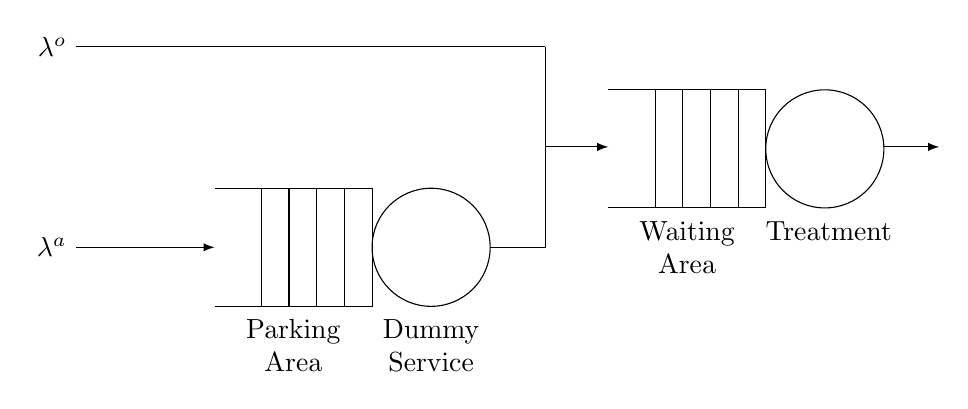
\begin{tikzpicture}[>=latex]
        % the rectangle with vertical rules (Queue 1)
        \draw (0,0) -- ++(2cm,0) -- ++(0,-1.5cm) -- ++(-2cm,0);
        \foreach \i in {1,...,4}
        \draw (2cm-\i*10pt,0) -- +(0,-1.5cm);
        
        % the circle (Queue 1)
        \draw (2.75,-0.75cm) circle [radius=0.75cm];

        % the rectangle with vertical rules (Queue 2)
        \draw (5,1.25) -- ++(2cm,0) -- ++(0,-1.5cm) -- ++(-2cm,0);
        \foreach \i in {1,...,4}
        \draw (7cm-\i*10pt,1.25) -- +(0,-1.5cm);

        % the circle (Queue 2)
        \draw (7.75,0.5) circle [radius=0.75cm];

        % the arrows and labels (Queue 1+2)
        \draw[-] (3.5,-0.75) -- +(20pt,0);
        \draw[<-] (0,-0.75) -- +(-50pt,0) node[left] {\( \lambda^a \)};
        \draw[->] (8.5,0.525) -- +(20pt,0);
        \node[align=center] at (1cm,-2cm) {Parking \\ Area};
        \node[align=center] at (2.75cm,-2cm) {Dummy \\ Service};
        \node[align=center] at (6cm,-0.75cm) {Waiting \\ Area};
        \node[align=center] at (7.8cm,-0.75cm) {Treatment \\ };
        
        \draw (4.2, 1.8) -- +(-169.5pt,0) node[left] {\( \lambda^o \)};
        \draw (4.2, 1.8) -- (4.2, -0.75);
        \draw[->] (4.2, 0.525) -- (5, 0.525);

    \end{tikzpicture}
\end{figure}


\begin{figure}
    \centering
    \begin{tikzpicture}[-, node distance = 1cm, auto, every node/.style={scale=0.5}]

        % Variables
        \tikzmath{
            let \altdist = 1.5cm;
            let \minsz = 1.5cm;
        }

        % First Line
        \node[state, minimum size=1.5cm] (zero) {(0,0)};
        \node[state, minimum size=1.5cm,  right=of zero] (one) {(0,1)};
        \node[draw=none, minimum size=1.5cm, right=of one] (two) {\dots};
        \node[state, minimum size=1.5cm, right=of two] (three) {(0,T)};
        \node[state, node distance = \altdist, minimum size=\minsz, right=of three] (four) {(0,T+1)};
        \node[draw=none, node distance = \altdist, minimum size=\minsz, right=of four] (five) {\dots};
        \node[state, node distance = \altdist, minimum size=\minsz, right=of five] (six) {(0,C)};
        \node[draw=none, minimum size=\minsz, right=of six] (seven) {\dots};

        % Second Line
        \node[state, minimum size=\minsz, below=of three] (three_one) {(1,T)};
        \node[state, minimum size=\minsz, below=of four] (four_one) {(1,T+1)};
        \node[draw=none, minimum size=\minsz, below=of five] (five_one) {\dots};
        \node[state, node distance = \altdist, minimum size=\minsz, right=of five_one] (six_one) {(1,C)};
        \node[draw=none, minimum size=\minsz, right=of six_one] (seven_one) {\dots};

        % Third Line
        \node[state, minimum size=\minsz, below=of three_one] (three_two) {(2,T)};
        \node[state, minimum size=\minsz, below=of four_one] (four_two) {(2,T+1)};
        \node[draw=none, minimum size=\minsz, below=of five_one] (five_two) {\dots};
        \node[state, node distance = \altdist, minimum size=\minsz, right=of five_two] (six_two) {(2,C)};
        \node[draw=none, minimum size=\minsz, right=of six_two] (seven_two) {\dots};

        % Fourth line
        \node[draw=none, minimum size=\minsz, below=of three_two] (three_three) {\vdots};
        \node[draw=none, minimum size=\minsz, below=of four_two] (four_three) {\vdots};
        \node[draw=none, minimum size=\minsz, below=of five_two] (five_three) {};
        \node[draw=none, node distance = \altdist, minimum size=\minsz, right=of five_three] (six_three) {\vdots};

        \draw[every loop]
            % First Horizontal Edges
            (zero) edge[bend left] node {\( \Lambda \)} (one)
            (one) edge[bend left] node [above] {\( \mu \)} (zero)
            (one) edge[bend left] node {\( \Lambda \)} (two)
            (two) edge[bend left] node [above] {\( 2 \mu \)} (one)
            (two) edge[bend left] node {\( \Lambda \)} (three)
            (three) edge[bend left] node [above] {\( T \mu \)} (two)
            (three) edge[bend left] node {\( \lambda^o \)} (four)
            (four) edge[bend left] node [above] {\( (T+1) \mu \)} (three)
            (four) edge[bend left] node {\( \lambda^o \)} (five)
            (five) edge[bend left] node [above] {\( (T+2) \mu \)} (four)
            (five) edge[bend left] node {\( \lambda^o \)} (six)
            (six) edge[bend left] node [above] {\( C\mu \)} (five)
            (six) edge[bend left] node {\( \lambda^o \)} (seven)
            (seven) edge[bend left] node [above] {\( C\mu \)} (six)

            % Second Horizontal Edges
            (three_one) edge[bend left] node {\( \lambda^o \)} (four_one)
            (four_one) edge[bend left] node [above] {\( (T+1) \mu \)} (three_one)
            (four_one) edge[bend left] node {\( \lambda^o \)} (five_one)
            (five_one) edge[bend left] node [above] {\( (T+2) \mu \)} (four_one)
            (five_one) edge[bend left] node {\( \lambda^o \)} (six_one)
            (six_one) edge[bend left] node [above] {\( C\mu \)} (five_one)
            (six_one) edge[bend left] node {\( \lambda^o \)} (seven_one)
            (seven_one) edge[bend left] node [above] {\( C\mu \)} (six_one)

            % Third Horizontal Edges
            (three_two) edge[bend left] node {\( \lambda^o \)} (four_two)
            (four_two) edge[bend left] node [above] {\( (T+1) \mu \)} (three_two)
            (four_two) edge[bend left] node {\( \lambda^o \)} (five_two)
            (five_two) edge[bend left] node [above] {\( (T+2) \mu \)} (four_two)
            (five_two) edge[bend left] node {\( \lambda^o \)} (six_two)
            (six_two) edge[bend left] node [above] {\( C\mu \)} (five_two)
            (six_two) edge[bend left] node {\( \lambda^o \)} (seven_two)
            (seven_two) edge[bend left] node [above] {\( C\mu \)} (six_two)

            % First Vertical Edges
            (three) edge[bend left] node {\( \lambda^A \)} (three_one)
            (three_one) edge[bend left] node {\( T \mu \)} (three)
            (three_one) edge[bend left] node {\( \lambda^A \)} (three_two)
            (three_two) edge[bend left] node {\( T\mu \)} (three_one)
            (three_two) edge[bend left] node {\( \lambda^A \)} (three_three)
            (three_three) edge[bend left] node {\( T\mu \)} (three_two)

            % Second Vertical Edges
            (four) edge node {\( \lambda^A \)} (four_one)
            (four_one) edge node {\( \lambda^A \)} (four_two)
            (four_two) edge node {\( \lambda^A \)} (four_three)

            %Third Vertical Edges
            (six) edge node {\( \lambda^A \)} (six_one)
            (six_one) edge node {\( \lambda^A \)} (six_two)
            (six_two) edge node {\( \lambda^A \)} (six_three)
            ;       
    \end{tikzpicture}
    \caption{Markov chains} 
    \label{Markov_2}
\end{figure}



\begin{figure}
    \centering
    \begin{tikzpicture}[-, node distance = 1cm, auto, every node/.style={scale=0.4}]

        % Variables
        \tikzmath{
            let \altdist = 1cm;
            let \minsz = 1.5cm;
        }

        % First Line
        \node[state, minimum size=1.5cm] (zero) {(0,0)};
        \node[state, minimum size=1.5cm,  right=of zero] (one) {(0,1)};
        \node[draw=none, minimum size=1.5cm, right=of one] (two) {\dots};
        \node[state, minimum size=1.5cm, right=of two] (three) {(0,T)};
        \node[state, node distance = \altdist, minimum size=\minsz, right=of three] (four) {(0,T+1)};
        \node[draw=none, minimum size=\minsz, right=of four] (five) {\dots};
        \node[draw=none, minimum size=\minsz, right=of five] (six) {\vdots};
        \node[draw=none, minimum size=\minsz, right=of six] (seven) {\dots};
        \node[state, minimum size=\minsz, right=of seven] (eight) {(0,C)};
        \node[draw=none, minimum size=\minsz, right=of eight] (nine) {\dots};


        % Second Line
        \node[state, minimum size=\minsz, below=of three] (three_one) {(1,T)};
        \node[state, minimum size=\minsz, below=of four] (four_one) {(1,T+1)};
        \node[draw=none, minimum size=\minsz, below=of five] (five_one) {\dots};
        \node[state, node distance = \altdist, minimum size=\minsz, right=of five_one] (six_one) {\( (u_i, v_i) \)};
        \node[draw=none, minimum size=\minsz, right=of six_one] (seven_one) {\dots};
        \node[state, node distance = \altdist, minimum size=\minsz, right=of seven_one] (eight_one) {(1,C)};
        \node[draw=none, minimum size=\minsz, right=of eight_one] (nine_one) {\dots};
        

        % Third Line
        \node[state, minimum size=\minsz, below=of three_one] (three_two) {(2,T)};
        \node[state, minimum size=\minsz, below=of four_one] (four_two) {(2,T+1)};
        \node[draw=none, minimum size=\minsz, below=of five_one] (five_two) {\dots};
        \node[draw=none, node distance = \altdist, minimum size=\minsz, right=of five_two] (six_two) {\vdots};
        \node[draw=none, minimum size=\minsz, right=of six_two] (seven_two) {\dots};
        \node[state, node distance = \altdist, minimum size=\minsz, right=of seven_two] (eight_two) {(2,C)};
        \node[draw=none, minimum size=\minsz, right=of eight_two] (nine_two) {\dots};

        % Fourth line
        \node[draw=none, minimum size=\minsz, below=of three_two] (three_three) {\vdots};
        \node[draw=none, minimum size=\minsz, below=of four_two] (four_three) {\vdots};
        \node[draw=none, minimum size=\minsz, below=of five_two] (five_three) {};
        \node[draw=none, node distance = \altdist, minimum size=\minsz, right=of five_three] (six_three) {};
        \node[draw=none, node distance = \altdist, minimum size=\minsz, below=of eight_two] (eight_three) {\vdots};


        \draw[every loop]
            % First Horizontal Edges
            (zero) edge[bend left] node {\( \Lambda \)} (one)
            (one) edge[bend left] node {\( \mu \)} (zero)
            (one) edge[bend left] node {\( \Lambda \)} (two)
            (two) edge[bend left] node {\( 2 \mu \)} (one)
            (two) edge[bend left] node {\( \Lambda \)} (three)
            (three) edge[bend left] node {\( T \mu \)} (two)
            (three) edge[bend left] node {\( \lambda^o \)} (four)
            (four) edge[bend left] node {\( (T+1) \mu \)} (three)
            (four) edge[bend left] node {\( \lambda^o \)} (five)
            (five) edge[bend left] node {\( (T+2) \mu \)} (four)
            % (five) edge[bend left] node {\( \lambda^o \)} (six)
            % (six) edge[bend left] node [above] {\( C\mu \)} (five)
            % (six) edge[bend left] node {\( \lambda^o \)} (seven)
            % (seven) edge[bend left] node [above] {\( C\mu \)} (six)
            (seven) edge[bend left] node {\( \lambda^o \)} (eight)
            (eight) edge[bend left] node {\( C\mu \)} (seven)
            (eight) edge[bend left] node {\( \lambda^o \)} (nine)
            (nine) edge[bend left] node {\( C\mu \)} (eight)

            % Second Horizontal Edges
            (three_one) edge[bend left] node {\(\lambda^o\)} (four_one)
            (four_one) edge[bend left] node {\( (T+1) \mu \)} (three_one)
            (four_one) edge[bend left] node {\( \lambda^o \)} (five_one)
            (five_one) edge[bend left] node {\( (T+2) \mu \)} (four_one)
            (five_one) edge[bend left] node {\( \lambda^o \)} (six_one)
            (six_one) edge[bend left] node {\( v_i\mu \)} (five_one)
            (six_one) edge[bend left] node {\( \lambda^o \)} (seven_one)
            (seven_one) edge[bend left] node {\( (v_i+1)\mu \)} (six_one)
            (seven_one) edge[bend left] node {\( \lambda^o \)} (eight_one)
            (eight_one) edge[bend left] node {\( C\mu \)} (seven_one)
            (eight_one) edge[bend left] node {\( \lambda^o \)} (nine_one)
            (nine_one) edge[bend left] node {\( C\mu \)} (eight_one)

            % Third Horizontal Edges
            (three_two) edge[bend left] node {\( \lambda^o \)} (four_two)
            (four_two) edge[bend left] node {\( (T+1) \mu \)} (three_two)
            (four_two) edge[bend left] node {\( \lambda^o \)} (five_two)
            (five_two) edge[bend left] node {\( (T+2) \mu \)} (four_two)
            % (five_two) edge[bend left] node {\( \lambda^o \)} (six_two)
            % (six_two) edge[bend left] node [above] {\( C\mu \)} (five_two)
            % (six_two) edge[bend left] node {\( \lambda^o \)} (seven_two)
            % (seven_two) edge[bend left] node [above] {\( C\mu \)} (six_two)
            (seven_two) edge[bend left] node {\( \lambda^o \)} (eight_two)
            (eight_two) edge[bend left] node {\( C\mu \)} (seven_two)
            (eight_two) edge[bend left] node {\( \lambda^o \)} (nine_two)
            (nine_two) edge[bend left] node {\( C\mu \)} (eight_two)

            % First Vertical Edges
            (three) edge[bend left] node {\( \lambda^A \)} (three_one)
            (three_one) edge[bend left] node {\( T \mu \)} (three)
            (three_one) edge[bend left] node {\( \lambda^A \)} (three_two)
            (three_two) edge[bend left] node {\( T\mu \)} (three_one)
            (three_two) edge[bend left] node {\( \lambda^A \)} (three_three)
            (three_three) edge[bend left] node {\( T\mu \)} (three_two)

            % Second Vertical Edges
            (four) edge node {\( \lambda^A \)} (four_one)
            (four_one) edge node {\( \lambda^A \)} (four_two)
            (four_two) edge node {\( \lambda^A \)} (four_three)

            % Third Vertical Edges
            (six) edge node {\( \lambda^A \)} (six_one)
            (six_one) edge node {\( \lambda^A \)} (six_two)
            % (six_two) edge node {\( \lambda^A \)} (six_three)

            % Fourth Vertical Edges
            (eight) edge node {\( \lambda^A \)} (eight_one)
            (eight_one) edge node {\( \lambda^A \)} (eight_two)
            (eight_two) edge node {\( \lambda^A \)} (eight_three)
            ;       
    \end{tikzpicture}
    \caption{Markov chains} 
    \label{Markov_3}
\end{figure}


\begin{figure}
    \centering
    \begin{tikzpicture}[-, node distance = 0.9cm, auto, every node/.style={scale=0.5}]

        % Variables
        \tikzmath{
            let \initdist = 0.5cm;
            let \altdist = 1.2cm;
            let \minsz = 1.6cm;
            let \leftOne = -0.8;
            let \rightOne = 2.2;
            let \upOne = 0.8;
            let \downOne = -2.2;
            let \leftTwo = 2.25;
            let \rightTwo = 14.2;
            let \upTwo = -2.35;
            let \downTwo = -8.8;
        }

        % % Rectangle for S1
        % \draw[ultra thin, dashed] (\leftOne, \downOne) -- (\leftOne, \upOne);
        % \draw[ultra thin, dashed] (\leftOne, \upOne) -- (\rightOne, \upOne);
        % \draw[ultra thin, dashed] (\rightOne, \upOne) -- node {\Huge{\( \quad S_1 \)}}(\rightOne, \downOne);
        % \draw[ultra thin, dashed] (\rightOne, \downOne) -- (\leftOne, \downOne);

        % % Rectangle for S2
        % \draw[ultra thin, dashed] (\leftTwo, \downTwo) -- node {\Huge{\( S_2 \quad \)}}(\leftTwo, \upTwo);
        % \draw[ultra thin, dashed] (\leftTwo, \upTwo) -- (\rightTwo, \upTwo);
        % \draw[ultra thin, dashed] (\rightTwo, \upTwo) -- (\rightTwo, \downTwo);
        % \draw[ultra thin, dashed] (\rightTwo, \downTwo) -- (\leftTwo, \downTwo);

        % First Line
        \node[state, minimum size=1.5cm] (zero) {(0,0)};
        \node[state, node distance = \initdist, minimum size=\minsz, below right=of zero] (one) {(0,1)};
        \node[draw=none, node distance = \initdist, minimum size=\minsz, below right=of one] (two) {\textbf{\( \ddots \)}};
        \node[state, node distance = \initdist, minimum size=\minsz, below right=of two] (three) {(0,T)};
        \node[state, node distance = \altdist, minimum size=\minsz, right=of three] (four) {(0,T+1)};
        \node[draw=none, node distance = \altdist, minimum size=\minsz, right=of four] (five) {\textbf{\dots}};
        \node[draw=none, minimum size=\minsz, right=of five] (six) {\textbf{\vdots}};
        \node[draw=none, minimum size=\minsz, right=of six] (seven) {\textbf{\dots}};
        \node[state, minimum size=\minsz, right=of seven] (eight) {(0,C)};
        \node[draw=none, minimum size=\minsz, right=of eight] (nine) {\textbf{\dots}};


        % Second Line
        \node[state, minimum size=\minsz, below=of three] (three_one) {(1,T)};
        \node[state, minimum size=\minsz, below=of four] (four_one) {(1,T+1)};
        \node[draw=none, minimum size=\minsz, below=of five] (five_one) {\textbf{\dots}};
        \node[state, minimum size=\minsz, right=of five_one] (six_one) {\( (u_i, v_i) \)};
        \node[draw=none, minimum size=\minsz, right=of six_one] (seven_one) {\textbf{\dots}};
        \node[state, minimum size=\minsz, right=of seven_one] (eight_one) {(1,C)};
        \node[draw=none, minimum size=\minsz, right=of eight_one] (nine_one) {\textbf{\dots}};
        

        % Third Line
        \node[state, minimum size=\minsz, below=of three_one] (three_two) {(2,T)};
        \node[state, minimum size=\minsz, below=of four_one] (four_two) {(2,T+1)};
        \node[draw=none, minimum size=\minsz, below=of five_one] (five_two) {\textbf{\dots}};
        \node[draw=none, minimum size=\minsz, right=of five_two] (six_two) {\textbf{\vdots}};
        \node[draw=none, minimum size=\minsz, right=of six_two] (seven_two) {\textbf{\dots}};
        \node[state, minimum size=\minsz, right=of seven_two] (eight_two) {(2,C)};
        \node[draw=none, minimum size=\minsz, right=of eight_two] (nine_two) {\textbf{\dots}};

        % Fourth line
        \node[draw=none, node distance = \altdist, minimum size=\minsz, below=of three_two] (three_three) {\textbf{\vdots}};
        \node[draw=none, node distance = \altdist, minimum size=\minsz, below=of four_two] (four_three) {\textbf{\vdots}};
        \node[draw=none, node distance = \altdist, minimum size=\minsz, below=of five_two] (five_three) {};
        \node[draw=none, node distance = \altdist, minimum size=\minsz, below=of six_two] (six_three) {};
        \node[draw=none, node distance = \altdist, minimum size=\minsz, below=of eight_two] (eight_three) {\textbf{\vdots}};


        \draw[every loop]
            % First Horizontal Edges
            (zero) edge[bend left] node {\( \Lambda \)} (one)
            (one) edge[bend left] node {\( \mu \)} (zero)
            (one) edge[bend left] node {\( \Lambda \)} (two)
            (two) edge[bend left] node {\( 2 \mu \)} (one)
            (two) edge[bend left] node {\( \Lambda \)} (three)
            (three) edge[bend left] node {\( T \mu \)} (two)
            (three) edge[bend left] node {\( \lambda^o \)} (four)
            (four) edge[bend left] node {\( (T+1) \mu \)} (three)
            (four) edge[bend left] node {\( \lambda^o \)} (five)
            (five) edge[bend left] node {\( (T+2) \mu \)} (four)
            % (five) edge[bend left] node {\( \lambda^o \)} (six)
            % (six) edge[bend left] node [above] {\( C\mu \)} (five)
            % (six) edge[bend left] node {\( \lambda^o \)} (seven)
            % (seven) edge[bend left] node [above] {\( C\mu \)} (six)
            (seven) edge[bend left] node {\( \lambda^o \)} (eight)
            (eight) edge[bend left] node {\( C\mu \)} (seven)
            (eight) edge[bend left] node {\( \lambda^o \)} (nine)
            (nine) edge[bend left] node {\( C\mu \)} (eight)

            % Second Horizontal Edges
            (three_one) edge[bend left] node {\( \lambda^o \)} (four_one)
            (four_one) edge[bend left] node {\( (T+1) \mu \)} (three_one)
            (four_one) edge[bend left] node {\( \lambda^o \)} (five_one)
            (five_one) edge[bend left] node {\( (T+2) \mu \)} (four_one)
            (five_one) edge[bend left] node {\( \lambda^o \)} (six_one)
            (six_one) edge[bend left] node {\( v_i\mu \)} (five_one)
            (six_one) edge[bend left] node {\( \lambda^o \)} (seven_one)
            (seven_one) edge[bend left] node {\( (v_i+1)\mu \)} (six_one)
            (seven_one) edge[bend left] node {\( \lambda^o \)} (eight_one)
            (eight_one) edge[bend left] node {\( C\mu \)} (seven_one)
            (eight_one) edge[bend left] node {\( \lambda^o \)} (nine_one)
            (nine_one) edge[bend left] node {\( C\mu \)} (eight_one)

            % Third Horizontal Edges
            (three_two) edge[bend left] node {\( \lambda^o \)} (four_two)
            (four_two) edge[bend left] node [below] {\( (T+1) \mu \)} (three_two)
            (four_two) edge[bend left] node {\( \lambda^o \)} (five_two)
            (five_two) edge[bend left] node {\( (T+2) \mu \)} (four_two)
            % (five_two) edge[bend left] node {\( \lambda^o \)} (six_two)
            % (six_two) edge[bend left] node [above] {\( C\mu \)} (five_two)
            % (six_two) edge[bend left] node {\( \lambda^o \)} (seven_two)
            % (seven_two) edge[bend left] node [above] {\( C\mu \)} (six_two)
            (seven_two) edge[bend left] node {\( \lambda^o \)} (eight_two)
            (eight_two) edge[bend left] node {\( C\mu \)} (seven_two)
            (eight_two) edge[bend left] node {\( \lambda^o \)} (nine_two)
            (nine_two) edge[bend left] node {\( C\mu \)} (eight_two)

            % First Vertical Edges
            (three) edge[bend left] node {\( \lambda^A \)} (three_one)
            (three_one) edge[bend left] node {\( T \mu \)} (three)
            (three_one) edge[bend left] node {\( \lambda^A \)} (three_two)
            (three_two) edge[bend left] node {\( T\mu \)} (three_one)
            (three_two) edge[bend left] node {\( \lambda^A \)} (three_three)
            (three_three) edge[bend left] node {\( T\mu \)} (three_two)

            % Second Vertical Edges
            (four) edge node {\( \lambda^A \)} (four_one)
            (four_one) edge node {\( \lambda^A \)} (four_two)
            (four_two) edge node {\( \lambda^A \)} (four_three)

            % Third Vertical Edges
            (six) edge node {\( \lambda^A \)} (six_one)
            (six_one) edge node {\( \lambda^A \)} (six_two)
            % (six_two) edge node {\( \lambda^A \)} (six_three)

            % Fourth Vertical Edges
            (eight) edge node {\( \lambda^A \)} (eight_one)
            (eight_one) edge node {\( \lambda^A \)} (eight_two)
            (eight_two) edge node {\( \lambda^A \)} (eight_three)
            ;       
    \end{tikzpicture}
    \caption{Markov chains} 
    \label{Markov_4}
\end{figure}




\begin{figure}
    \centering
    \begin{tikzpicture}[-, node distance = 0.9cm, auto, every node/.style={scale=0.7}]

        % Markov chain variables
        \tikzmath{
            let \initdist = 0.5cm;
            let \altdist = 1.2cm;
            let \minsz = 1.6cm;
        }

        % S_1 and S_2 rectangles
        \tikzmath{
            let \leftOne = -0.8;
            let \rightOne = 2.7;
            let \upOne = 0.8;
            let \downOne = -2.7;
            let \leftTwo = 2.8;
            let \rightTwo = 13;
            let \upTwo = -2.95;
            let \downTwo = -16.4;
        }

        % General case variables
        \tikzmath{
            let \GCsmallx = 8.3;
            let \GCsmally = -9.5;
            let \GCbigx = 4.1;
            let \GCbigy = -11.8;
        }

        % % Rectangle for S1
        % \draw[ultra thin, dashed] (\leftOne, \downOne) -- (\leftOne, \upOne);
        % \draw[ultra thin, dashed] (\leftOne, \upOne) -- (\rightOne, \upOne);
        % \draw[ultra thin, dashed] (\rightOne, \upOne) -- node {\Huge{\( \quad S_1 \)}}(\rightOne, \downOne);
        % \draw[ultra thin, dashed] (\rightOne, \downOne) -- (\leftOne, \downOne);

        % % Rectangle for S2
        % \draw[ultra thin, dashed] (\leftTwo, \downTwo) -- node {\Huge{\( S_2 \quad \)}}(\leftTwo, \upTwo);
        % \draw[ultra thin, dashed] (\leftTwo, \upTwo) -- (\rightTwo, \upTwo);
        % \draw[ultra thin, dashed] (\rightTwo, \upTwo) -- (\rightTwo, \downTwo);
        % \draw[ultra thin, dashed] (\rightTwo, \downTwo) -- (\leftTwo, \downTwo);

        % Small square of general case
        \draw [thick] (\GCsmallx, \GCsmally) -- node {} (\GCsmallx + 0.4, \GCsmally);
        \draw [thick] (\GCsmallx + 0.4, \GCsmally) -- node {} (\GCsmallx + 0.4, \GCsmally - 0.4);
        \draw [thick] (\GCsmallx + 0.4, \GCsmally - 0.4) -- node {} (\GCsmallx, \GCsmally - 0.4);
        \draw [thick] (\GCsmallx, \GCsmally - 0.4) -- node {} (\GCsmallx, \GCsmally);


        % Dashed lines to from small square to big one 
        \draw [ultra thin] (\GCsmallx, \GCsmally) -- node {} (\GCbigx, \GCbigy);
        \draw [ultra thin] (\GCsmallx + 0.4, \GCsmally) -- node {} (\GCbigx + 4, \GCbigy);
        \draw [ultra thin] (\GCsmallx, \GCsmally - 0.4) -- node {} (7, \GCbigy);
        \draw [ultra thin] (\GCsmallx + 0.4, \GCsmally - 0.4) -- node {} (\GCbigx + 4, \GCbigy - 4);
        
        % Big Square of general case
        \draw [ultra thick] (\GCbigx, \GCbigy) -- node {} (\GCbigx + 4, \GCbigy);
        \draw [ultra thick] (\GCbigx + 4, \GCbigy) -- node {} (\GCbigx + 4, \GCbigy - 4);
        \draw [ultra thick] (\GCbigx + 4, \GCbigy - 4) -- node {General Case} (\GCbigx, \GCbigy - 4);
        \draw [ultra thick] (\GCbigx, \GCbigy - 4) -- node {} (\GCbigx, \GCbigy);

        % First Line
        \node[state, minimum size=1.5cm] (zero) {(0,0)};
        \node[state, node distance = \initdist, minimum size=\minsz, below right=of zero] (one) {(0,1)};
        \node[draw=none, node distance = \initdist, minimum size=\minsz, below right=of one] (two) {\textbf{\( \ddots \)}};
        \node[state, node distance = \initdist, minimum size=\minsz, below right=of two] (three) {(0,T)};
        \node[state, node distance = \altdist, minimum size=\minsz, right=of three] (four) {(0,T+1)};
        \node[draw=none, node distance = \altdist, minimum size=\minsz, right=of four] (five) {\textbf{\dots}};
        \node[state, minimum size=\minsz, right=of five] (six) {(0,C)};
        \node[draw=none, minimum size=\minsz, right=of six] (seven) {\textbf{\dots}};

        % Second Line
        \node[state, minimum size=\minsz, below=of three] (three_one) {(1,T)};
        \node[state, minimum size=\minsz, below=of four] (four_one) {(1,T+1)};
        \node[draw=none, minimum size=\minsz, below=of five] (five_one) {\textbf{\dots}};
        \node[state, minimum size=\minsz, right=of five_one] (six_one) {(1,C)};
        \node[draw=none, minimum size=\minsz, right=of six_one] (seven_one) {\textbf{\dots}};
        
        % Third Line
        \node[state, minimum size=\minsz, below=of three_one] (three_two) {(2,T)};
        \node[state, minimum size=\minsz, below=of four_one] (four_two) {(2,T+1)};
        \node[draw=none, minimum size=\minsz, below=of five_one] (five_two) {\textbf{\dots}};
        \node[state, minimum size=\minsz, right=of five_two] (six_two) {(2,C)};
        \node[draw=none, minimum size=\minsz, right=of six_two] (seven_two) {\textbf{\dots}};

        % Fourth line
        \node[draw=none, node distance = \altdist, minimum size=\minsz, below=of three_two] (three_three) {\textbf{\vdots}};
        \node[draw=none, node distance = \altdist, minimum size=\minsz, below=of four_two] (four_three) {\textbf{\vdots}};
        \node[draw=none, node distance = 2cm, minimum size=\minsz, below=of five_two] (five_three) {};
        \node[draw=none, node distance = \altdist, minimum size=\minsz, below=of six_two] (six_three) {\textbf{\vdots}};

        % Fifth line
        % \node[state, node distance = \altdist, minimum size=\minsz, below=of five_three] (general_case_mid) {\( (u_i, v_i) \)};
        \node[draw=none, node distance = 0.3cm, minimum size=\minsz, below=of four_three] (general_case_up) {};
        \node[state, node distance = \altdist, minimum size=\minsz, below=of general_case_up] (general_case_mid) {\( (u_i, v_i) \)};

        \node[draw=none, node distance = \altdist, minimum size=\minsz, below=of general_case_mid] (general_case_down) {};
        \node[draw=none, node distance = \altdist, minimum size=\minsz, left=of general_case_mid] (general_case_left) {};
        \node[draw=none, node distance = \altdist, minimum size=\minsz, right=of general_case_mid] (general_case_right) {};

        \draw[every loop]
            % First Horizontal Edges
            (zero) edge[bend left] node {\( \Lambda \)} (one)
            (one) edge[bend left] node {\( \mu \)} (zero)
            (one) edge[bend left] node {\( \Lambda \)} (two)
            (two) edge[bend left] node {\( 2 \mu \)} (one)
            (two) edge[bend left] node {\( \Lambda \)} (three)
            (three) edge[bend left] node {\( T \mu \)} (two)
            (three) edge[bend left] node {\( \lambda^o \)} (four)
            (four) edge[bend left] node {\( (T+1) \mu \)} (three)
            (four) edge[bend left] node {\( \lambda^o \)} (five)
            (five) edge[bend left] node {\( (T+2) \mu \)} (four)
            (five) edge[bend left] node {\( \lambda^o \)} (six)
            (six) edge[bend left] node {\( C\mu \)} (five)
            (six) edge[bend left] node {\( \lambda^o \)} (seven)
            (seven) edge[bend left] node {\( C\mu \)} (six)

            % Second Horizontal Edges
            (three_one) edge[bend left] node {\( \lambda^o \)} (four_one)
            (four_one) edge[bend left] node {\( (T+1) \mu \)} (three_one)
            (four_one) edge[bend left] node {\( \lambda^o \)} (five_one)
            (five_one) edge[bend left] node {\( (T+2) \mu \)} (four_one)
            (five_one) edge[bend left] node {\( \lambda^o \)} (six_one)
            (six_one) edge[bend left] node {\( C\mu \)} (five_one)
            (six_one) edge[bend left] node {\( \lambda^o \)} (seven_one)
            (seven_one) edge[bend left] node {\( C\mu \)} (six_one)

            % Third Horizontal Edges
            (three_two) edge[bend left] node {\( \lambda^o \)} (four_two)
            (four_two) edge[bend left] node [below] {\( (T+1) \mu \)} (three_two)
            (four_two) edge[bend left] node {\( \lambda^o \)} (five_two)
            (five_two) edge[bend left] node {\( (T+2) \mu \)} (four_two)
            (five_two) edge[bend left] node {\( \lambda^o \)} (six_two)
            (six_two) edge[bend left] node {\( C\mu \)} (five_two)
            (six_two) edge[bend left] node {\( \lambda^o \)} (seven_two)
            (seven_two) edge[bend left] node {\( C\mu \)} (six_two)

            % First Vertical Edges
            (three) edge[bend left] node {\( \lambda^A \)} (three_one)
            (three_one) edge[bend left] node {\( T \mu \)} (three)
            (three_one) edge[bend left] node {\( \lambda^A \)} (three_two)
            (three_two) edge[bend left] node {\( T\mu \)} (three_one)
            (three_two) edge[bend left] node {\( \lambda^A \)} (three_three)
            (three_three) edge[bend left] node {\( T\mu \)} (three_two)

            % Second Vertical Edges
            (four) edge node {\( \lambda^A \)} (four_one)
            (four_one) edge node {\( \lambda^A \)} (four_two)
            (four_two) edge node {\( \lambda^A \)} (four_three)

            % Fourth Vertical Edges
            (six) edge node {\( \lambda^A \)} (six_one)
            (six_one) edge node {\( \lambda^A \)} (six_two)
            (six_two) edge node {\( \lambda^A \)} (six_three)

            % General Case
            (general_case_left) edge[bend left] node {\( \lambda^o \)} (general_case_mid)
            (general_case_mid) edge[bend left] node {\( v_i \mu \)} (general_case_left)
            (general_case_right) edge[bend left] node {\( (v_i +1) \mu \)} (general_case_mid)
            (general_case_mid) edge[bend left] node {\( \lambda_o \)} (general_case_right)
            % (five_three) edge node {\( \lambda_A \)} (general_case_mid)
            (general_case_up) edge node {\( \lambda_A \)} (general_case_mid)
            (general_case_mid) edge node {\( \lambda_A \)} (general_case_down)
            ;
    \end{tikzpicture}
    \caption{Markov chain} 
    \label{Markov_5}
\end{figure}


        }
    \caption{\(C=1, T=3, N=5, M=2\)}
    \label{fig:Markov_1352_example_for_closed_form}
\end{figure}

In figure \ref{fig:Markov_1352_example_for_closed_form} an example of such a 
Markov model is shown where \(C=1\), \(T=3\) which means that the \textit{left 
arm} 
of the model has a length of \(3\), \(N=5\) that indicates that the right-most 
states \((u,v)\) are of the form \((u,5)\) and \(M=2\) that equivalently shows 
that the bottom states are of the form \((2,v)\).

\subsubsection{A graph theoretic model underling the Markov chain}

An additional approach that one may consider to get the state probabilities is 
the graph theoretical approach for state probabilities.
Thus, it can be assumed that a Markov chain model \(M\) can be translated as a 
weighted directed graph \(G_M = (V, E)\) where \(V=S\) from equation 
\ref{eq:state_space} and \((v_i, v_j)\in E\) if and only if \(q_{v_i, v_j}>0\). 
Furthermore, the weights are given by:
\[
    w(v_i, v_j) = q_{v_i, v_j}
\]

A \textit{directed spanning tree} of a directed graph is defined as a subset of 
the graph that visits all the vertices of the graph and does not include any cycles. 
Unlike undirected spanning trees, directed ones also have a root which means 
that a directed spanning tree that is rooted at a vertex \(v\) has to have a 
path from any other vertex to vertex \(v\). 
For example, consider the graph shown in figure \ref{fig:example_spanning_tree}.
The graph points out a spanning tree that is rooted at vertex 3.


\begin{figure}[h]
    \centering
    \begin{tikzpicture}
        \node[state](u1){1};
        \node[state, right=of u1](u2){2};
        \node[state, right=of u2](u3){3};
        \node[state, right=of u3](u4){4};
        \node[state, below=of u2](u5){5};
        \node[state, below=of u3](u6){6};
        \node[state, below=of u4](u7){7};
        \draw[->, thick] (u1) -- (u2);
        \draw[->, thick] (u2) -- (u3);
        \draw[->, thick] (u4) -- (u3);
        \draw[->, thick] (u5) -- (u2);
        \draw[->, thick] (u6) -- (u5);
        \draw[->, thick] (u7) -- (u6);
    \end{tikzpicture}
    \caption{Spanning tree of a graph rooted at vertex 3}
    \label{fig:example_spanning_tree}
\end{figure}

Additionally, let us denote the set of all spanning trees of \(G\) as \(T(G)\) 
and the subset of \(T(G)\) that includes only the spanning trees that are rooted 
at vertex \(v\) as \(T_v(G)\). 
The weight of a spanning tree \(t\) can be defined as the product of the weights 
of the edges it contains: 

\[w(t)=\prod_{e \in t} w(e)\]



\textbf{Theorem: Markov chain tree theorem} \cite{markov-chain-tree-theorem} \newline
\textit{Let M be an irreducible Markov chain on n states with stationary 
distribution \(\pi_1, \pi_2, \dots, \pi_n\). 
Let \(G_M\) be the directed graph associated with \(M\). 
Then the probability of being at state \(u\) is given by:}

\begin{equation}\label{markov-chain-tree-theorem}
    \pi_i = \frac{\sum_{t \in T_i(G_M)} w(t)}{\sum_{t \in T(G_M)}w(t)}
\end{equation}

Equation \ref{markov-chain-tree-theorem} states that the probability of being at
state \(u\) can be found by dividing the sum of the weights of all trees in 
\(T_u(G)\) by the sum of the weights of all tress in \(T(G)\). 
Let us ignore the denominator of that fraction for now and focus only on the 
numerator denoted as \(\tilde{\pi}_i=\sum_{t \in T_i(G_M)} w(t)\)

 

\newpage
\subsubsection{Spanning Trees rooted at \((0,0)\)}

Let us now consider some examples of spanning trees that are rooted at \((0,0)\). 
For each of the following examples the complete graph \(G\) is shown, then all 
possible trees of \(T_{(0,0)}(G)\) along with the weight associated with each 
spanning tree.
As well as this, the sum of all the weights of the spanning trees denoted by 
\(\tilde{\pi}_{(0,0)}\) is also included.

\begin{figure}[h]
    \centering
    \section{Figures that might be useful}
\begin{figure}[h]
    \centering
    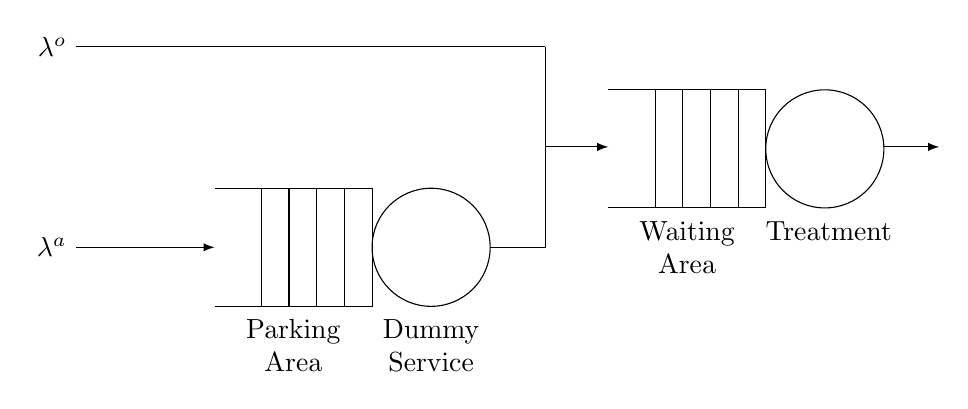
\begin{tikzpicture}[>=latex]
        % the rectangle with vertical rules (Queue 1)
        \draw (0,0) -- ++(2cm,0) -- ++(0,-1.5cm) -- ++(-2cm,0);
        \foreach \i in {1,...,4}
        \draw (2cm-\i*10pt,0) -- +(0,-1.5cm);
        
        % the circle (Queue 1)
        \draw (2.75,-0.75cm) circle [radius=0.75cm];

        % the rectangle with vertical rules (Queue 2)
        \draw (5,1.25) -- ++(2cm,0) -- ++(0,-1.5cm) -- ++(-2cm,0);
        \foreach \i in {1,...,4}
        \draw (7cm-\i*10pt,1.25) -- +(0,-1.5cm);

        % the circle (Queue 2)
        \draw (7.75,0.5) circle [radius=0.75cm];

        % the arrows and labels (Queue 1+2)
        \draw[-] (3.5,-0.75) -- +(20pt,0);
        \draw[<-] (0,-0.75) -- +(-50pt,0) node[left] {\( \lambda^a \)};
        \draw[->] (8.5,0.525) -- +(20pt,0);
        \node[align=center] at (1cm,-2cm) {Parking \\ Area};
        \node[align=center] at (2.75cm,-2cm) {Dummy \\ Service};
        \node[align=center] at (6cm,-0.75cm) {Waiting \\ Area};
        \node[align=center] at (7.8cm,-0.75cm) {Treatment \\ };
        
        \draw (4.2, 1.8) -- +(-169.5pt,0) node[left] {\( \lambda^o \)};
        \draw (4.2, 1.8) -- (4.2, -0.75);
        \draw[->] (4.2, 0.525) -- (5, 0.525);

    \end{tikzpicture}
\end{figure}


\begin{figure}
    \centering
    \begin{tikzpicture}[-, node distance = 1cm, auto, every node/.style={scale=0.5}]

        % Variables
        \tikzmath{
            let \altdist = 1.5cm;
            let \minsz = 1.5cm;
        }

        % First Line
        \node[state, minimum size=1.5cm] (zero) {(0,0)};
        \node[state, minimum size=1.5cm,  right=of zero] (one) {(0,1)};
        \node[draw=none, minimum size=1.5cm, right=of one] (two) {\dots};
        \node[state, minimum size=1.5cm, right=of two] (three) {(0,T)};
        \node[state, node distance = \altdist, minimum size=\minsz, right=of three] (four) {(0,T+1)};
        \node[draw=none, node distance = \altdist, minimum size=\minsz, right=of four] (five) {\dots};
        \node[state, node distance = \altdist, minimum size=\minsz, right=of five] (six) {(0,C)};
        \node[draw=none, minimum size=\minsz, right=of six] (seven) {\dots};

        % Second Line
        \node[state, minimum size=\minsz, below=of three] (three_one) {(1,T)};
        \node[state, minimum size=\minsz, below=of four] (four_one) {(1,T+1)};
        \node[draw=none, minimum size=\minsz, below=of five] (five_one) {\dots};
        \node[state, node distance = \altdist, minimum size=\minsz, right=of five_one] (six_one) {(1,C)};
        \node[draw=none, minimum size=\minsz, right=of six_one] (seven_one) {\dots};

        % Third Line
        \node[state, minimum size=\minsz, below=of three_one] (three_two) {(2,T)};
        \node[state, minimum size=\minsz, below=of four_one] (four_two) {(2,T+1)};
        \node[draw=none, minimum size=\minsz, below=of five_one] (five_two) {\dots};
        \node[state, node distance = \altdist, minimum size=\minsz, right=of five_two] (six_two) {(2,C)};
        \node[draw=none, minimum size=\minsz, right=of six_two] (seven_two) {\dots};

        % Fourth line
        \node[draw=none, minimum size=\minsz, below=of three_two] (three_three) {\vdots};
        \node[draw=none, minimum size=\minsz, below=of four_two] (four_three) {\vdots};
        \node[draw=none, minimum size=\minsz, below=of five_two] (five_three) {};
        \node[draw=none, node distance = \altdist, minimum size=\minsz, right=of five_three] (six_three) {\vdots};

        \draw[every loop]
            % First Horizontal Edges
            (zero) edge[bend left] node {\( \Lambda \)} (one)
            (one) edge[bend left] node [above] {\( \mu \)} (zero)
            (one) edge[bend left] node {\( \Lambda \)} (two)
            (two) edge[bend left] node [above] {\( 2 \mu \)} (one)
            (two) edge[bend left] node {\( \Lambda \)} (three)
            (three) edge[bend left] node [above] {\( T \mu \)} (two)
            (three) edge[bend left] node {\( \lambda^o \)} (four)
            (four) edge[bend left] node [above] {\( (T+1) \mu \)} (three)
            (four) edge[bend left] node {\( \lambda^o \)} (five)
            (five) edge[bend left] node [above] {\( (T+2) \mu \)} (four)
            (five) edge[bend left] node {\( \lambda^o \)} (six)
            (six) edge[bend left] node [above] {\( C\mu \)} (five)
            (six) edge[bend left] node {\( \lambda^o \)} (seven)
            (seven) edge[bend left] node [above] {\( C\mu \)} (six)

            % Second Horizontal Edges
            (three_one) edge[bend left] node {\( \lambda^o \)} (four_one)
            (four_one) edge[bend left] node [above] {\( (T+1) \mu \)} (three_one)
            (four_one) edge[bend left] node {\( \lambda^o \)} (five_one)
            (five_one) edge[bend left] node [above] {\( (T+2) \mu \)} (four_one)
            (five_one) edge[bend left] node {\( \lambda^o \)} (six_one)
            (six_one) edge[bend left] node [above] {\( C\mu \)} (five_one)
            (six_one) edge[bend left] node {\( \lambda^o \)} (seven_one)
            (seven_one) edge[bend left] node [above] {\( C\mu \)} (six_one)

            % Third Horizontal Edges
            (three_two) edge[bend left] node {\( \lambda^o \)} (four_two)
            (four_two) edge[bend left] node [above] {\( (T+1) \mu \)} (three_two)
            (four_two) edge[bend left] node {\( \lambda^o \)} (five_two)
            (five_two) edge[bend left] node [above] {\( (T+2) \mu \)} (four_two)
            (five_two) edge[bend left] node {\( \lambda^o \)} (six_two)
            (six_two) edge[bend left] node [above] {\( C\mu \)} (five_two)
            (six_two) edge[bend left] node {\( \lambda^o \)} (seven_two)
            (seven_two) edge[bend left] node [above] {\( C\mu \)} (six_two)

            % First Vertical Edges
            (three) edge[bend left] node {\( \lambda^A \)} (three_one)
            (three_one) edge[bend left] node {\( T \mu \)} (three)
            (three_one) edge[bend left] node {\( \lambda^A \)} (three_two)
            (three_two) edge[bend left] node {\( T\mu \)} (three_one)
            (three_two) edge[bend left] node {\( \lambda^A \)} (three_three)
            (three_three) edge[bend left] node {\( T\mu \)} (three_two)

            % Second Vertical Edges
            (four) edge node {\( \lambda^A \)} (four_one)
            (four_one) edge node {\( \lambda^A \)} (four_two)
            (four_two) edge node {\( \lambda^A \)} (four_three)

            %Third Vertical Edges
            (six) edge node {\( \lambda^A \)} (six_one)
            (six_one) edge node {\( \lambda^A \)} (six_two)
            (six_two) edge node {\( \lambda^A \)} (six_three)
            ;       
    \end{tikzpicture}
    \caption{Markov chains} 
    \label{Markov_2}
\end{figure}



\begin{figure}
    \centering
    \begin{tikzpicture}[-, node distance = 1cm, auto, every node/.style={scale=0.4}]

        % Variables
        \tikzmath{
            let \altdist = 1cm;
            let \minsz = 1.5cm;
        }

        % First Line
        \node[state, minimum size=1.5cm] (zero) {(0,0)};
        \node[state, minimum size=1.5cm,  right=of zero] (one) {(0,1)};
        \node[draw=none, minimum size=1.5cm, right=of one] (two) {\dots};
        \node[state, minimum size=1.5cm, right=of two] (three) {(0,T)};
        \node[state, node distance = \altdist, minimum size=\minsz, right=of three] (four) {(0,T+1)};
        \node[draw=none, minimum size=\minsz, right=of four] (five) {\dots};
        \node[draw=none, minimum size=\minsz, right=of five] (six) {\vdots};
        \node[draw=none, minimum size=\minsz, right=of six] (seven) {\dots};
        \node[state, minimum size=\minsz, right=of seven] (eight) {(0,C)};
        \node[draw=none, minimum size=\minsz, right=of eight] (nine) {\dots};


        % Second Line
        \node[state, minimum size=\minsz, below=of three] (three_one) {(1,T)};
        \node[state, minimum size=\minsz, below=of four] (four_one) {(1,T+1)};
        \node[draw=none, minimum size=\minsz, below=of five] (five_one) {\dots};
        \node[state, node distance = \altdist, minimum size=\minsz, right=of five_one] (six_one) {\( (u_i, v_i) \)};
        \node[draw=none, minimum size=\minsz, right=of six_one] (seven_one) {\dots};
        \node[state, node distance = \altdist, minimum size=\minsz, right=of seven_one] (eight_one) {(1,C)};
        \node[draw=none, minimum size=\minsz, right=of eight_one] (nine_one) {\dots};
        

        % Third Line
        \node[state, minimum size=\minsz, below=of three_one] (three_two) {(2,T)};
        \node[state, minimum size=\minsz, below=of four_one] (four_two) {(2,T+1)};
        \node[draw=none, minimum size=\minsz, below=of five_one] (five_two) {\dots};
        \node[draw=none, node distance = \altdist, minimum size=\minsz, right=of five_two] (six_two) {\vdots};
        \node[draw=none, minimum size=\minsz, right=of six_two] (seven_two) {\dots};
        \node[state, node distance = \altdist, minimum size=\minsz, right=of seven_two] (eight_two) {(2,C)};
        \node[draw=none, minimum size=\minsz, right=of eight_two] (nine_two) {\dots};

        % Fourth line
        \node[draw=none, minimum size=\minsz, below=of three_two] (three_three) {\vdots};
        \node[draw=none, minimum size=\minsz, below=of four_two] (four_three) {\vdots};
        \node[draw=none, minimum size=\minsz, below=of five_two] (five_three) {};
        \node[draw=none, node distance = \altdist, minimum size=\minsz, right=of five_three] (six_three) {};
        \node[draw=none, node distance = \altdist, minimum size=\minsz, below=of eight_two] (eight_three) {\vdots};


        \draw[every loop]
            % First Horizontal Edges
            (zero) edge[bend left] node {\( \Lambda \)} (one)
            (one) edge[bend left] node {\( \mu \)} (zero)
            (one) edge[bend left] node {\( \Lambda \)} (two)
            (two) edge[bend left] node {\( 2 \mu \)} (one)
            (two) edge[bend left] node {\( \Lambda \)} (three)
            (three) edge[bend left] node {\( T \mu \)} (two)
            (three) edge[bend left] node {\( \lambda^o \)} (four)
            (four) edge[bend left] node {\( (T+1) \mu \)} (three)
            (four) edge[bend left] node {\( \lambda^o \)} (five)
            (five) edge[bend left] node {\( (T+2) \mu \)} (four)
            % (five) edge[bend left] node {\( \lambda^o \)} (six)
            % (six) edge[bend left] node [above] {\( C\mu \)} (five)
            % (six) edge[bend left] node {\( \lambda^o \)} (seven)
            % (seven) edge[bend left] node [above] {\( C\mu \)} (six)
            (seven) edge[bend left] node {\( \lambda^o \)} (eight)
            (eight) edge[bend left] node {\( C\mu \)} (seven)
            (eight) edge[bend left] node {\( \lambda^o \)} (nine)
            (nine) edge[bend left] node {\( C\mu \)} (eight)

            % Second Horizontal Edges
            (three_one) edge[bend left] node {\(\lambda^o\)} (four_one)
            (four_one) edge[bend left] node {\( (T+1) \mu \)} (three_one)
            (four_one) edge[bend left] node {\( \lambda^o \)} (five_one)
            (five_one) edge[bend left] node {\( (T+2) \mu \)} (four_one)
            (five_one) edge[bend left] node {\( \lambda^o \)} (six_one)
            (six_one) edge[bend left] node {\( v_i\mu \)} (five_one)
            (six_one) edge[bend left] node {\( \lambda^o \)} (seven_one)
            (seven_one) edge[bend left] node {\( (v_i+1)\mu \)} (six_one)
            (seven_one) edge[bend left] node {\( \lambda^o \)} (eight_one)
            (eight_one) edge[bend left] node {\( C\mu \)} (seven_one)
            (eight_one) edge[bend left] node {\( \lambda^o \)} (nine_one)
            (nine_one) edge[bend left] node {\( C\mu \)} (eight_one)

            % Third Horizontal Edges
            (three_two) edge[bend left] node {\( \lambda^o \)} (four_two)
            (four_two) edge[bend left] node {\( (T+1) \mu \)} (three_two)
            (four_two) edge[bend left] node {\( \lambda^o \)} (five_two)
            (five_two) edge[bend left] node {\( (T+2) \mu \)} (four_two)
            % (five_two) edge[bend left] node {\( \lambda^o \)} (six_two)
            % (six_two) edge[bend left] node [above] {\( C\mu \)} (five_two)
            % (six_two) edge[bend left] node {\( \lambda^o \)} (seven_two)
            % (seven_two) edge[bend left] node [above] {\( C\mu \)} (six_two)
            (seven_two) edge[bend left] node {\( \lambda^o \)} (eight_two)
            (eight_two) edge[bend left] node {\( C\mu \)} (seven_two)
            (eight_two) edge[bend left] node {\( \lambda^o \)} (nine_two)
            (nine_two) edge[bend left] node {\( C\mu \)} (eight_two)

            % First Vertical Edges
            (three) edge[bend left] node {\( \lambda^A \)} (three_one)
            (three_one) edge[bend left] node {\( T \mu \)} (three)
            (three_one) edge[bend left] node {\( \lambda^A \)} (three_two)
            (three_two) edge[bend left] node {\( T\mu \)} (three_one)
            (three_two) edge[bend left] node {\( \lambda^A \)} (three_three)
            (three_three) edge[bend left] node {\( T\mu \)} (three_two)

            % Second Vertical Edges
            (four) edge node {\( \lambda^A \)} (four_one)
            (four_one) edge node {\( \lambda^A \)} (four_two)
            (four_two) edge node {\( \lambda^A \)} (four_three)

            % Third Vertical Edges
            (six) edge node {\( \lambda^A \)} (six_one)
            (six_one) edge node {\( \lambda^A \)} (six_two)
            % (six_two) edge node {\( \lambda^A \)} (six_three)

            % Fourth Vertical Edges
            (eight) edge node {\( \lambda^A \)} (eight_one)
            (eight_one) edge node {\( \lambda^A \)} (eight_two)
            (eight_two) edge node {\( \lambda^A \)} (eight_three)
            ;       
    \end{tikzpicture}
    \caption{Markov chains} 
    \label{Markov_3}
\end{figure}


\begin{figure}
    \centering
    \begin{tikzpicture}[-, node distance = 0.9cm, auto, every node/.style={scale=0.5}]

        % Variables
        \tikzmath{
            let \initdist = 0.5cm;
            let \altdist = 1.2cm;
            let \minsz = 1.6cm;
            let \leftOne = -0.8;
            let \rightOne = 2.2;
            let \upOne = 0.8;
            let \downOne = -2.2;
            let \leftTwo = 2.25;
            let \rightTwo = 14.2;
            let \upTwo = -2.35;
            let \downTwo = -8.8;
        }

        % % Rectangle for S1
        % \draw[ultra thin, dashed] (\leftOne, \downOne) -- (\leftOne, \upOne);
        % \draw[ultra thin, dashed] (\leftOne, \upOne) -- (\rightOne, \upOne);
        % \draw[ultra thin, dashed] (\rightOne, \upOne) -- node {\Huge{\( \quad S_1 \)}}(\rightOne, \downOne);
        % \draw[ultra thin, dashed] (\rightOne, \downOne) -- (\leftOne, \downOne);

        % % Rectangle for S2
        % \draw[ultra thin, dashed] (\leftTwo, \downTwo) -- node {\Huge{\( S_2 \quad \)}}(\leftTwo, \upTwo);
        % \draw[ultra thin, dashed] (\leftTwo, \upTwo) -- (\rightTwo, \upTwo);
        % \draw[ultra thin, dashed] (\rightTwo, \upTwo) -- (\rightTwo, \downTwo);
        % \draw[ultra thin, dashed] (\rightTwo, \downTwo) -- (\leftTwo, \downTwo);

        % First Line
        \node[state, minimum size=1.5cm] (zero) {(0,0)};
        \node[state, node distance = \initdist, minimum size=\minsz, below right=of zero] (one) {(0,1)};
        \node[draw=none, node distance = \initdist, minimum size=\minsz, below right=of one] (two) {\textbf{\( \ddots \)}};
        \node[state, node distance = \initdist, minimum size=\minsz, below right=of two] (three) {(0,T)};
        \node[state, node distance = \altdist, minimum size=\minsz, right=of three] (four) {(0,T+1)};
        \node[draw=none, node distance = \altdist, minimum size=\minsz, right=of four] (five) {\textbf{\dots}};
        \node[draw=none, minimum size=\minsz, right=of five] (six) {\textbf{\vdots}};
        \node[draw=none, minimum size=\minsz, right=of six] (seven) {\textbf{\dots}};
        \node[state, minimum size=\minsz, right=of seven] (eight) {(0,C)};
        \node[draw=none, minimum size=\minsz, right=of eight] (nine) {\textbf{\dots}};


        % Second Line
        \node[state, minimum size=\minsz, below=of three] (three_one) {(1,T)};
        \node[state, minimum size=\minsz, below=of four] (four_one) {(1,T+1)};
        \node[draw=none, minimum size=\minsz, below=of five] (five_one) {\textbf{\dots}};
        \node[state, minimum size=\minsz, right=of five_one] (six_one) {\( (u_i, v_i) \)};
        \node[draw=none, minimum size=\minsz, right=of six_one] (seven_one) {\textbf{\dots}};
        \node[state, minimum size=\minsz, right=of seven_one] (eight_one) {(1,C)};
        \node[draw=none, minimum size=\minsz, right=of eight_one] (nine_one) {\textbf{\dots}};
        

        % Third Line
        \node[state, minimum size=\minsz, below=of three_one] (three_two) {(2,T)};
        \node[state, minimum size=\minsz, below=of four_one] (four_two) {(2,T+1)};
        \node[draw=none, minimum size=\minsz, below=of five_one] (five_two) {\textbf{\dots}};
        \node[draw=none, minimum size=\minsz, right=of five_two] (six_two) {\textbf{\vdots}};
        \node[draw=none, minimum size=\minsz, right=of six_two] (seven_two) {\textbf{\dots}};
        \node[state, minimum size=\minsz, right=of seven_two] (eight_two) {(2,C)};
        \node[draw=none, minimum size=\minsz, right=of eight_two] (nine_two) {\textbf{\dots}};

        % Fourth line
        \node[draw=none, node distance = \altdist, minimum size=\minsz, below=of three_two] (three_three) {\textbf{\vdots}};
        \node[draw=none, node distance = \altdist, minimum size=\minsz, below=of four_two] (four_three) {\textbf{\vdots}};
        \node[draw=none, node distance = \altdist, minimum size=\minsz, below=of five_two] (five_three) {};
        \node[draw=none, node distance = \altdist, minimum size=\minsz, below=of six_two] (six_three) {};
        \node[draw=none, node distance = \altdist, minimum size=\minsz, below=of eight_two] (eight_three) {\textbf{\vdots}};


        \draw[every loop]
            % First Horizontal Edges
            (zero) edge[bend left] node {\( \Lambda \)} (one)
            (one) edge[bend left] node {\( \mu \)} (zero)
            (one) edge[bend left] node {\( \Lambda \)} (two)
            (two) edge[bend left] node {\( 2 \mu \)} (one)
            (two) edge[bend left] node {\( \Lambda \)} (three)
            (three) edge[bend left] node {\( T \mu \)} (two)
            (three) edge[bend left] node {\( \lambda^o \)} (four)
            (four) edge[bend left] node {\( (T+1) \mu \)} (three)
            (four) edge[bend left] node {\( \lambda^o \)} (five)
            (five) edge[bend left] node {\( (T+2) \mu \)} (four)
            % (five) edge[bend left] node {\( \lambda^o \)} (six)
            % (six) edge[bend left] node [above] {\( C\mu \)} (five)
            % (six) edge[bend left] node {\( \lambda^o \)} (seven)
            % (seven) edge[bend left] node [above] {\( C\mu \)} (six)
            (seven) edge[bend left] node {\( \lambda^o \)} (eight)
            (eight) edge[bend left] node {\( C\mu \)} (seven)
            (eight) edge[bend left] node {\( \lambda^o \)} (nine)
            (nine) edge[bend left] node {\( C\mu \)} (eight)

            % Second Horizontal Edges
            (three_one) edge[bend left] node {\( \lambda^o \)} (four_one)
            (four_one) edge[bend left] node {\( (T+1) \mu \)} (three_one)
            (four_one) edge[bend left] node {\( \lambda^o \)} (five_one)
            (five_one) edge[bend left] node {\( (T+2) \mu \)} (four_one)
            (five_one) edge[bend left] node {\( \lambda^o \)} (six_one)
            (six_one) edge[bend left] node {\( v_i\mu \)} (five_one)
            (six_one) edge[bend left] node {\( \lambda^o \)} (seven_one)
            (seven_one) edge[bend left] node {\( (v_i+1)\mu \)} (six_one)
            (seven_one) edge[bend left] node {\( \lambda^o \)} (eight_one)
            (eight_one) edge[bend left] node {\( C\mu \)} (seven_one)
            (eight_one) edge[bend left] node {\( \lambda^o \)} (nine_one)
            (nine_one) edge[bend left] node {\( C\mu \)} (eight_one)

            % Third Horizontal Edges
            (three_two) edge[bend left] node {\( \lambda^o \)} (four_two)
            (four_two) edge[bend left] node [below] {\( (T+1) \mu \)} (three_two)
            (four_two) edge[bend left] node {\( \lambda^o \)} (five_two)
            (five_two) edge[bend left] node {\( (T+2) \mu \)} (four_two)
            % (five_two) edge[bend left] node {\( \lambda^o \)} (six_two)
            % (six_two) edge[bend left] node [above] {\( C\mu \)} (five_two)
            % (six_two) edge[bend left] node {\( \lambda^o \)} (seven_two)
            % (seven_two) edge[bend left] node [above] {\( C\mu \)} (six_two)
            (seven_two) edge[bend left] node {\( \lambda^o \)} (eight_two)
            (eight_two) edge[bend left] node {\( C\mu \)} (seven_two)
            (eight_two) edge[bend left] node {\( \lambda^o \)} (nine_two)
            (nine_two) edge[bend left] node {\( C\mu \)} (eight_two)

            % First Vertical Edges
            (three) edge[bend left] node {\( \lambda^A \)} (three_one)
            (three_one) edge[bend left] node {\( T \mu \)} (three)
            (three_one) edge[bend left] node {\( \lambda^A \)} (three_two)
            (three_two) edge[bend left] node {\( T\mu \)} (three_one)
            (three_two) edge[bend left] node {\( \lambda^A \)} (three_three)
            (three_three) edge[bend left] node {\( T\mu \)} (three_two)

            % Second Vertical Edges
            (four) edge node {\( \lambda^A \)} (four_one)
            (four_one) edge node {\( \lambda^A \)} (four_two)
            (four_two) edge node {\( \lambda^A \)} (four_three)

            % Third Vertical Edges
            (six) edge node {\( \lambda^A \)} (six_one)
            (six_one) edge node {\( \lambda^A \)} (six_two)
            % (six_two) edge node {\( \lambda^A \)} (six_three)

            % Fourth Vertical Edges
            (eight) edge node {\( \lambda^A \)} (eight_one)
            (eight_one) edge node {\( \lambda^A \)} (eight_two)
            (eight_two) edge node {\( \lambda^A \)} (eight_three)
            ;       
    \end{tikzpicture}
    \caption{Markov chains} 
    \label{Markov_4}
\end{figure}




\begin{figure}
    \centering
    \begin{tikzpicture}[-, node distance = 0.9cm, auto, every node/.style={scale=0.7}]

        % Markov chain variables
        \tikzmath{
            let \initdist = 0.5cm;
            let \altdist = 1.2cm;
            let \minsz = 1.6cm;
        }

        % S_1 and S_2 rectangles
        \tikzmath{
            let \leftOne = -0.8;
            let \rightOne = 2.7;
            let \upOne = 0.8;
            let \downOne = -2.7;
            let \leftTwo = 2.8;
            let \rightTwo = 13;
            let \upTwo = -2.95;
            let \downTwo = -16.4;
        }

        % General case variables
        \tikzmath{
            let \GCsmallx = 8.3;
            let \GCsmally = -9.5;
            let \GCbigx = 4.1;
            let \GCbigy = -11.8;
        }

        % % Rectangle for S1
        % \draw[ultra thin, dashed] (\leftOne, \downOne) -- (\leftOne, \upOne);
        % \draw[ultra thin, dashed] (\leftOne, \upOne) -- (\rightOne, \upOne);
        % \draw[ultra thin, dashed] (\rightOne, \upOne) -- node {\Huge{\( \quad S_1 \)}}(\rightOne, \downOne);
        % \draw[ultra thin, dashed] (\rightOne, \downOne) -- (\leftOne, \downOne);

        % % Rectangle for S2
        % \draw[ultra thin, dashed] (\leftTwo, \downTwo) -- node {\Huge{\( S_2 \quad \)}}(\leftTwo, \upTwo);
        % \draw[ultra thin, dashed] (\leftTwo, \upTwo) -- (\rightTwo, \upTwo);
        % \draw[ultra thin, dashed] (\rightTwo, \upTwo) -- (\rightTwo, \downTwo);
        % \draw[ultra thin, dashed] (\rightTwo, \downTwo) -- (\leftTwo, \downTwo);

        % Small square of general case
        \draw [thick] (\GCsmallx, \GCsmally) -- node {} (\GCsmallx + 0.4, \GCsmally);
        \draw [thick] (\GCsmallx + 0.4, \GCsmally) -- node {} (\GCsmallx + 0.4, \GCsmally - 0.4);
        \draw [thick] (\GCsmallx + 0.4, \GCsmally - 0.4) -- node {} (\GCsmallx, \GCsmally - 0.4);
        \draw [thick] (\GCsmallx, \GCsmally - 0.4) -- node {} (\GCsmallx, \GCsmally);


        % Dashed lines to from small square to big one 
        \draw [ultra thin] (\GCsmallx, \GCsmally) -- node {} (\GCbigx, \GCbigy);
        \draw [ultra thin] (\GCsmallx + 0.4, \GCsmally) -- node {} (\GCbigx + 4, \GCbigy);
        \draw [ultra thin] (\GCsmallx, \GCsmally - 0.4) -- node {} (7, \GCbigy);
        \draw [ultra thin] (\GCsmallx + 0.4, \GCsmally - 0.4) -- node {} (\GCbigx + 4, \GCbigy - 4);
        
        % Big Square of general case
        \draw [ultra thick] (\GCbigx, \GCbigy) -- node {} (\GCbigx + 4, \GCbigy);
        \draw [ultra thick] (\GCbigx + 4, \GCbigy) -- node {} (\GCbigx + 4, \GCbigy - 4);
        \draw [ultra thick] (\GCbigx + 4, \GCbigy - 4) -- node {General Case} (\GCbigx, \GCbigy - 4);
        \draw [ultra thick] (\GCbigx, \GCbigy - 4) -- node {} (\GCbigx, \GCbigy);

        % First Line
        \node[state, minimum size=1.5cm] (zero) {(0,0)};
        \node[state, node distance = \initdist, minimum size=\minsz, below right=of zero] (one) {(0,1)};
        \node[draw=none, node distance = \initdist, minimum size=\minsz, below right=of one] (two) {\textbf{\( \ddots \)}};
        \node[state, node distance = \initdist, minimum size=\minsz, below right=of two] (three) {(0,T)};
        \node[state, node distance = \altdist, minimum size=\minsz, right=of three] (four) {(0,T+1)};
        \node[draw=none, node distance = \altdist, minimum size=\minsz, right=of four] (five) {\textbf{\dots}};
        \node[state, minimum size=\minsz, right=of five] (six) {(0,C)};
        \node[draw=none, minimum size=\minsz, right=of six] (seven) {\textbf{\dots}};

        % Second Line
        \node[state, minimum size=\minsz, below=of three] (three_one) {(1,T)};
        \node[state, minimum size=\minsz, below=of four] (four_one) {(1,T+1)};
        \node[draw=none, minimum size=\minsz, below=of five] (five_one) {\textbf{\dots}};
        \node[state, minimum size=\minsz, right=of five_one] (six_one) {(1,C)};
        \node[draw=none, minimum size=\minsz, right=of six_one] (seven_one) {\textbf{\dots}};
        
        % Third Line
        \node[state, minimum size=\minsz, below=of three_one] (three_two) {(2,T)};
        \node[state, minimum size=\minsz, below=of four_one] (four_two) {(2,T+1)};
        \node[draw=none, minimum size=\minsz, below=of five_one] (five_two) {\textbf{\dots}};
        \node[state, minimum size=\minsz, right=of five_two] (six_two) {(2,C)};
        \node[draw=none, minimum size=\minsz, right=of six_two] (seven_two) {\textbf{\dots}};

        % Fourth line
        \node[draw=none, node distance = \altdist, minimum size=\minsz, below=of three_two] (three_three) {\textbf{\vdots}};
        \node[draw=none, node distance = \altdist, minimum size=\minsz, below=of four_two] (four_three) {\textbf{\vdots}};
        \node[draw=none, node distance = 2cm, minimum size=\minsz, below=of five_two] (five_three) {};
        \node[draw=none, node distance = \altdist, minimum size=\minsz, below=of six_two] (six_three) {\textbf{\vdots}};

        % Fifth line
        % \node[state, node distance = \altdist, minimum size=\minsz, below=of five_three] (general_case_mid) {\( (u_i, v_i) \)};
        \node[draw=none, node distance = 0.3cm, minimum size=\minsz, below=of four_three] (general_case_up) {};
        \node[state, node distance = \altdist, minimum size=\minsz, below=of general_case_up] (general_case_mid) {\( (u_i, v_i) \)};

        \node[draw=none, node distance = \altdist, minimum size=\minsz, below=of general_case_mid] (general_case_down) {};
        \node[draw=none, node distance = \altdist, minimum size=\minsz, left=of general_case_mid] (general_case_left) {};
        \node[draw=none, node distance = \altdist, minimum size=\minsz, right=of general_case_mid] (general_case_right) {};

        \draw[every loop]
            % First Horizontal Edges
            (zero) edge[bend left] node {\( \Lambda \)} (one)
            (one) edge[bend left] node {\( \mu \)} (zero)
            (one) edge[bend left] node {\( \Lambda \)} (two)
            (two) edge[bend left] node {\( 2 \mu \)} (one)
            (two) edge[bend left] node {\( \Lambda \)} (three)
            (three) edge[bend left] node {\( T \mu \)} (two)
            (three) edge[bend left] node {\( \lambda^o \)} (four)
            (four) edge[bend left] node {\( (T+1) \mu \)} (three)
            (four) edge[bend left] node {\( \lambda^o \)} (five)
            (five) edge[bend left] node {\( (T+2) \mu \)} (four)
            (five) edge[bend left] node {\( \lambda^o \)} (six)
            (six) edge[bend left] node {\( C\mu \)} (five)
            (six) edge[bend left] node {\( \lambda^o \)} (seven)
            (seven) edge[bend left] node {\( C\mu \)} (six)

            % Second Horizontal Edges
            (three_one) edge[bend left] node {\( \lambda^o \)} (four_one)
            (four_one) edge[bend left] node {\( (T+1) \mu \)} (three_one)
            (four_one) edge[bend left] node {\( \lambda^o \)} (five_one)
            (five_one) edge[bend left] node {\( (T+2) \mu \)} (four_one)
            (five_one) edge[bend left] node {\( \lambda^o \)} (six_one)
            (six_one) edge[bend left] node {\( C\mu \)} (five_one)
            (six_one) edge[bend left] node {\( \lambda^o \)} (seven_one)
            (seven_one) edge[bend left] node {\( C\mu \)} (six_one)

            % Third Horizontal Edges
            (three_two) edge[bend left] node {\( \lambda^o \)} (four_two)
            (four_two) edge[bend left] node [below] {\( (T+1) \mu \)} (three_two)
            (four_two) edge[bend left] node {\( \lambda^o \)} (five_two)
            (five_two) edge[bend left] node {\( (T+2) \mu \)} (four_two)
            (five_two) edge[bend left] node {\( \lambda^o \)} (six_two)
            (six_two) edge[bend left] node {\( C\mu \)} (five_two)
            (six_two) edge[bend left] node {\( \lambda^o \)} (seven_two)
            (seven_two) edge[bend left] node {\( C\mu \)} (six_two)

            % First Vertical Edges
            (three) edge[bend left] node {\( \lambda^A \)} (three_one)
            (three_one) edge[bend left] node {\( T \mu \)} (three)
            (three_one) edge[bend left] node {\( \lambda^A \)} (three_two)
            (three_two) edge[bend left] node {\( T\mu \)} (three_one)
            (three_two) edge[bend left] node {\( \lambda^A \)} (three_three)
            (three_three) edge[bend left] node {\( T\mu \)} (three_two)

            % Second Vertical Edges
            (four) edge node {\( \lambda^A \)} (four_one)
            (four_one) edge node {\( \lambda^A \)} (four_two)
            (four_two) edge node {\( \lambda^A \)} (four_three)

            % Fourth Vertical Edges
            (six) edge node {\( \lambda^A \)} (six_one)
            (six_one) edge node {\( \lambda^A \)} (six_two)
            (six_two) edge node {\( \lambda^A \)} (six_three)

            % General Case
            (general_case_left) edge[bend left] node {\( \lambda^o \)} (general_case_mid)
            (general_case_mid) edge[bend left] node {\( v_i \mu \)} (general_case_left)
            (general_case_right) edge[bend left] node {\( (v_i +1) \mu \)} (general_case_mid)
            (general_case_mid) edge[bend left] node {\( \lambda_o \)} (general_case_right)
            % (five_three) edge node {\( \lambda_A \)} (general_case_mid)
            (general_case_up) edge node {\( \lambda_A \)} (general_case_mid)
            (general_case_mid) edge node {\( \lambda_A \)} (general_case_down)
            ;
    \end{tikzpicture}
    \caption{Markov chain} 
    \label{Markov_5}
\end{figure}


\end{figure}

\begin{multicols}{2}
    \begin{center}
        

\begin{tikzpicture}[-, node distance = 1cm, auto]
\node[state] (u0v0) {(0,0)};
\node[state, right=of u0v0] (u0v1) {(0,1)};
\draw[->](u0v1) edge node {\(\mu \)} (u0v0);
\node[state, below=of u0v1] (u1v1) {(1,1)};
\draw[->](u1v1) edge node {\(\mu \)} (u0v1);
\node[state, right=of u0v1] (u0v2) {(0,2)};
\node[state, right=of u1v1] (u1v2) {(1,2)};
\draw[->](u1v2) edge node {\(\mu \)} (u1v1);
\node[state, right=of u0v2] (u0v3) {(0,3)};
\node[state, right=of u1v2] (u1v3) {(1,3)};
\draw[->](u1v3) edge node {\(\mu \)} (u1v2);
\draw[->](u0v2) edge node {\(\lambda_2 \)} (u1v2);
\draw[->](u0v3) edge node {\(\lambda_2 \)} (u1v3);
\end{tikzpicture}
    \end{center}

    \begin{flalign*}
        \xrightarrow{\hspace*{2cm}} \hspace{1cm} \lambda_2 \mu^3
    \end{flalign*}
\end{multicols}


\begin{multicols}{2}
    \begin{center}
        

\begin{tikzpicture}[-, node distance = 1cm, auto]
\node[state] (u0v0) {(0,0)};
\node[state, right=of u0v0] (u0v1) {(0,1)};
\draw[->](u0v1) edge node {\(\mu \)} (u0v0);
\node[state, below=of u0v1] (u1v1) {(1,1)};
\draw[->](u1v1) edge node {\(\mu \)} (u0v1);
\node[state, right=of u0v1] (u0v2) {(0,2)};
\node[state, right=of u1v1] (u1v2) {(1,2)};
\draw[->](u1v2) edge node {\(\mu \)} (u1v1);
\node[state, right=of u0v2] (u0v3) {(0,3)};
\node[state, right=of u1v2] (u1v3) {(1,3)};
\draw[->](u1v3) edge node {\(\mu \)} (u1v2);
\draw[->](u0v2) edge node {\(\mu \)} (u0v1);
\draw[->](u0v3) edge node {\(\lambda_2 \)} (u1v3);
\end{tikzpicture}
    \end{center}

    \begin{flalign*}
        \xrightarrow{\hspace*{2cm}} \hspace{1cm} \mu^4
    \end{flalign*}
\end{multicols}

\begin{equation*}
    \tilde{\pi}_{(0,0)} = \mu^4 + \lambda_2 \mu^3
\end{equation*}



\newpage
\begin{figure}[h]
    \centering
    \section{Figures that might be useful}
\begin{figure}[h]
    \centering
    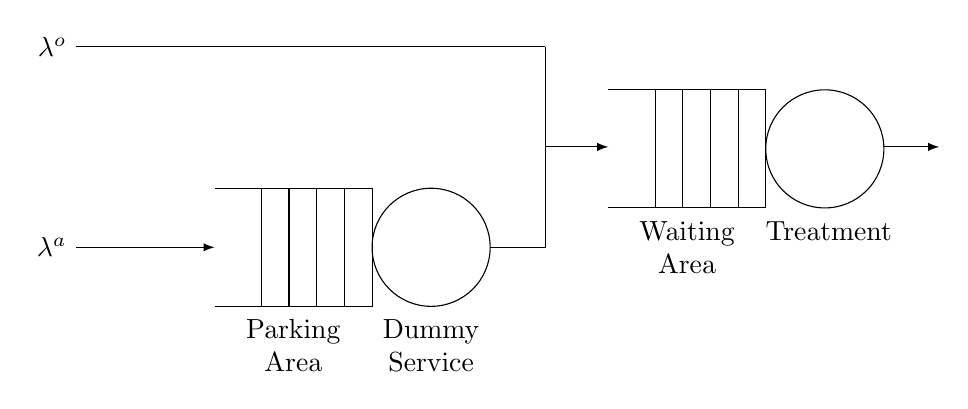
\begin{tikzpicture}[>=latex]
        % the rectangle with vertical rules (Queue 1)
        \draw (0,0) -- ++(2cm,0) -- ++(0,-1.5cm) -- ++(-2cm,0);
        \foreach \i in {1,...,4}
        \draw (2cm-\i*10pt,0) -- +(0,-1.5cm);
        
        % the circle (Queue 1)
        \draw (2.75,-0.75cm) circle [radius=0.75cm];

        % the rectangle with vertical rules (Queue 2)
        \draw (5,1.25) -- ++(2cm,0) -- ++(0,-1.5cm) -- ++(-2cm,0);
        \foreach \i in {1,...,4}
        \draw (7cm-\i*10pt,1.25) -- +(0,-1.5cm);

        % the circle (Queue 2)
        \draw (7.75,0.5) circle [radius=0.75cm];

        % the arrows and labels (Queue 1+2)
        \draw[-] (3.5,-0.75) -- +(20pt,0);
        \draw[<-] (0,-0.75) -- +(-50pt,0) node[left] {\( \lambda^a \)};
        \draw[->] (8.5,0.525) -- +(20pt,0);
        \node[align=center] at (1cm,-2cm) {Parking \\ Area};
        \node[align=center] at (2.75cm,-2cm) {Dummy \\ Service};
        \node[align=center] at (6cm,-0.75cm) {Waiting \\ Area};
        \node[align=center] at (7.8cm,-0.75cm) {Treatment \\ };
        
        \draw (4.2, 1.8) -- +(-169.5pt,0) node[left] {\( \lambda^o \)};
        \draw (4.2, 1.8) -- (4.2, -0.75);
        \draw[->] (4.2, 0.525) -- (5, 0.525);

    \end{tikzpicture}
\end{figure}


\begin{figure}
    \centering
    \begin{tikzpicture}[-, node distance = 1cm, auto, every node/.style={scale=0.5}]

        % Variables
        \tikzmath{
            let \altdist = 1.5cm;
            let \minsz = 1.5cm;
        }

        % First Line
        \node[state, minimum size=1.5cm] (zero) {(0,0)};
        \node[state, minimum size=1.5cm,  right=of zero] (one) {(0,1)};
        \node[draw=none, minimum size=1.5cm, right=of one] (two) {\dots};
        \node[state, minimum size=1.5cm, right=of two] (three) {(0,T)};
        \node[state, node distance = \altdist, minimum size=\minsz, right=of three] (four) {(0,T+1)};
        \node[draw=none, node distance = \altdist, minimum size=\minsz, right=of four] (five) {\dots};
        \node[state, node distance = \altdist, minimum size=\minsz, right=of five] (six) {(0,C)};
        \node[draw=none, minimum size=\minsz, right=of six] (seven) {\dots};

        % Second Line
        \node[state, minimum size=\minsz, below=of three] (three_one) {(1,T)};
        \node[state, minimum size=\minsz, below=of four] (four_one) {(1,T+1)};
        \node[draw=none, minimum size=\minsz, below=of five] (five_one) {\dots};
        \node[state, node distance = \altdist, minimum size=\minsz, right=of five_one] (six_one) {(1,C)};
        \node[draw=none, minimum size=\minsz, right=of six_one] (seven_one) {\dots};

        % Third Line
        \node[state, minimum size=\minsz, below=of three_one] (three_two) {(2,T)};
        \node[state, minimum size=\minsz, below=of four_one] (four_two) {(2,T+1)};
        \node[draw=none, minimum size=\minsz, below=of five_one] (five_two) {\dots};
        \node[state, node distance = \altdist, minimum size=\minsz, right=of five_two] (six_two) {(2,C)};
        \node[draw=none, minimum size=\minsz, right=of six_two] (seven_two) {\dots};

        % Fourth line
        \node[draw=none, minimum size=\minsz, below=of three_two] (three_three) {\vdots};
        \node[draw=none, minimum size=\minsz, below=of four_two] (four_three) {\vdots};
        \node[draw=none, minimum size=\minsz, below=of five_two] (five_three) {};
        \node[draw=none, node distance = \altdist, minimum size=\minsz, right=of five_three] (six_three) {\vdots};

        \draw[every loop]
            % First Horizontal Edges
            (zero) edge[bend left] node {\( \Lambda \)} (one)
            (one) edge[bend left] node [above] {\( \mu \)} (zero)
            (one) edge[bend left] node {\( \Lambda \)} (two)
            (two) edge[bend left] node [above] {\( 2 \mu \)} (one)
            (two) edge[bend left] node {\( \Lambda \)} (three)
            (three) edge[bend left] node [above] {\( T \mu \)} (two)
            (three) edge[bend left] node {\( \lambda^o \)} (four)
            (four) edge[bend left] node [above] {\( (T+1) \mu \)} (three)
            (four) edge[bend left] node {\( \lambda^o \)} (five)
            (five) edge[bend left] node [above] {\( (T+2) \mu \)} (four)
            (five) edge[bend left] node {\( \lambda^o \)} (six)
            (six) edge[bend left] node [above] {\( C\mu \)} (five)
            (six) edge[bend left] node {\( \lambda^o \)} (seven)
            (seven) edge[bend left] node [above] {\( C\mu \)} (six)

            % Second Horizontal Edges
            (three_one) edge[bend left] node {\( \lambda^o \)} (four_one)
            (four_one) edge[bend left] node [above] {\( (T+1) \mu \)} (three_one)
            (four_one) edge[bend left] node {\( \lambda^o \)} (five_one)
            (five_one) edge[bend left] node [above] {\( (T+2) \mu \)} (four_one)
            (five_one) edge[bend left] node {\( \lambda^o \)} (six_one)
            (six_one) edge[bend left] node [above] {\( C\mu \)} (five_one)
            (six_one) edge[bend left] node {\( \lambda^o \)} (seven_one)
            (seven_one) edge[bend left] node [above] {\( C\mu \)} (six_one)

            % Third Horizontal Edges
            (three_two) edge[bend left] node {\( \lambda^o \)} (four_two)
            (four_two) edge[bend left] node [above] {\( (T+1) \mu \)} (three_two)
            (four_two) edge[bend left] node {\( \lambda^o \)} (five_two)
            (five_two) edge[bend left] node [above] {\( (T+2) \mu \)} (four_two)
            (five_two) edge[bend left] node {\( \lambda^o \)} (six_two)
            (six_two) edge[bend left] node [above] {\( C\mu \)} (five_two)
            (six_two) edge[bend left] node {\( \lambda^o \)} (seven_two)
            (seven_two) edge[bend left] node [above] {\( C\mu \)} (six_two)

            % First Vertical Edges
            (three) edge[bend left] node {\( \lambda^A \)} (three_one)
            (three_one) edge[bend left] node {\( T \mu \)} (three)
            (three_one) edge[bend left] node {\( \lambda^A \)} (three_two)
            (three_two) edge[bend left] node {\( T\mu \)} (three_one)
            (three_two) edge[bend left] node {\( \lambda^A \)} (three_three)
            (three_three) edge[bend left] node {\( T\mu \)} (three_two)

            % Second Vertical Edges
            (four) edge node {\( \lambda^A \)} (four_one)
            (four_one) edge node {\( \lambda^A \)} (four_two)
            (four_two) edge node {\( \lambda^A \)} (four_three)

            %Third Vertical Edges
            (six) edge node {\( \lambda^A \)} (six_one)
            (six_one) edge node {\( \lambda^A \)} (six_two)
            (six_two) edge node {\( \lambda^A \)} (six_three)
            ;       
    \end{tikzpicture}
    \caption{Markov chains} 
    \label{Markov_2}
\end{figure}



\begin{figure}
    \centering
    \begin{tikzpicture}[-, node distance = 1cm, auto, every node/.style={scale=0.4}]

        % Variables
        \tikzmath{
            let \altdist = 1cm;
            let \minsz = 1.5cm;
        }

        % First Line
        \node[state, minimum size=1.5cm] (zero) {(0,0)};
        \node[state, minimum size=1.5cm,  right=of zero] (one) {(0,1)};
        \node[draw=none, minimum size=1.5cm, right=of one] (two) {\dots};
        \node[state, minimum size=1.5cm, right=of two] (three) {(0,T)};
        \node[state, node distance = \altdist, minimum size=\minsz, right=of three] (four) {(0,T+1)};
        \node[draw=none, minimum size=\minsz, right=of four] (five) {\dots};
        \node[draw=none, minimum size=\minsz, right=of five] (six) {\vdots};
        \node[draw=none, minimum size=\minsz, right=of six] (seven) {\dots};
        \node[state, minimum size=\minsz, right=of seven] (eight) {(0,C)};
        \node[draw=none, minimum size=\minsz, right=of eight] (nine) {\dots};


        % Second Line
        \node[state, minimum size=\minsz, below=of three] (three_one) {(1,T)};
        \node[state, minimum size=\minsz, below=of four] (four_one) {(1,T+1)};
        \node[draw=none, minimum size=\minsz, below=of five] (five_one) {\dots};
        \node[state, node distance = \altdist, minimum size=\minsz, right=of five_one] (six_one) {\( (u_i, v_i) \)};
        \node[draw=none, minimum size=\minsz, right=of six_one] (seven_one) {\dots};
        \node[state, node distance = \altdist, minimum size=\minsz, right=of seven_one] (eight_one) {(1,C)};
        \node[draw=none, minimum size=\minsz, right=of eight_one] (nine_one) {\dots};
        

        % Third Line
        \node[state, minimum size=\minsz, below=of three_one] (three_two) {(2,T)};
        \node[state, minimum size=\minsz, below=of four_one] (four_two) {(2,T+1)};
        \node[draw=none, minimum size=\minsz, below=of five_one] (five_two) {\dots};
        \node[draw=none, node distance = \altdist, minimum size=\minsz, right=of five_two] (six_two) {\vdots};
        \node[draw=none, minimum size=\minsz, right=of six_two] (seven_two) {\dots};
        \node[state, node distance = \altdist, minimum size=\minsz, right=of seven_two] (eight_two) {(2,C)};
        \node[draw=none, minimum size=\minsz, right=of eight_two] (nine_two) {\dots};

        % Fourth line
        \node[draw=none, minimum size=\minsz, below=of three_two] (three_three) {\vdots};
        \node[draw=none, minimum size=\minsz, below=of four_two] (four_three) {\vdots};
        \node[draw=none, minimum size=\minsz, below=of five_two] (five_three) {};
        \node[draw=none, node distance = \altdist, minimum size=\minsz, right=of five_three] (six_three) {};
        \node[draw=none, node distance = \altdist, minimum size=\minsz, below=of eight_two] (eight_three) {\vdots};


        \draw[every loop]
            % First Horizontal Edges
            (zero) edge[bend left] node {\( \Lambda \)} (one)
            (one) edge[bend left] node {\( \mu \)} (zero)
            (one) edge[bend left] node {\( \Lambda \)} (two)
            (two) edge[bend left] node {\( 2 \mu \)} (one)
            (two) edge[bend left] node {\( \Lambda \)} (three)
            (three) edge[bend left] node {\( T \mu \)} (two)
            (three) edge[bend left] node {\( \lambda^o \)} (four)
            (four) edge[bend left] node {\( (T+1) \mu \)} (three)
            (four) edge[bend left] node {\( \lambda^o \)} (five)
            (five) edge[bend left] node {\( (T+2) \mu \)} (four)
            % (five) edge[bend left] node {\( \lambda^o \)} (six)
            % (six) edge[bend left] node [above] {\( C\mu \)} (five)
            % (six) edge[bend left] node {\( \lambda^o \)} (seven)
            % (seven) edge[bend left] node [above] {\( C\mu \)} (six)
            (seven) edge[bend left] node {\( \lambda^o \)} (eight)
            (eight) edge[bend left] node {\( C\mu \)} (seven)
            (eight) edge[bend left] node {\( \lambda^o \)} (nine)
            (nine) edge[bend left] node {\( C\mu \)} (eight)

            % Second Horizontal Edges
            (three_one) edge[bend left] node {\(\lambda^o\)} (four_one)
            (four_one) edge[bend left] node {\( (T+1) \mu \)} (three_one)
            (four_one) edge[bend left] node {\( \lambda^o \)} (five_one)
            (five_one) edge[bend left] node {\( (T+2) \mu \)} (four_one)
            (five_one) edge[bend left] node {\( \lambda^o \)} (six_one)
            (six_one) edge[bend left] node {\( v_i\mu \)} (five_one)
            (six_one) edge[bend left] node {\( \lambda^o \)} (seven_one)
            (seven_one) edge[bend left] node {\( (v_i+1)\mu \)} (six_one)
            (seven_one) edge[bend left] node {\( \lambda^o \)} (eight_one)
            (eight_one) edge[bend left] node {\( C\mu \)} (seven_one)
            (eight_one) edge[bend left] node {\( \lambda^o \)} (nine_one)
            (nine_one) edge[bend left] node {\( C\mu \)} (eight_one)

            % Third Horizontal Edges
            (three_two) edge[bend left] node {\( \lambda^o \)} (four_two)
            (four_two) edge[bend left] node {\( (T+1) \mu \)} (three_two)
            (four_two) edge[bend left] node {\( \lambda^o \)} (five_two)
            (five_two) edge[bend left] node {\( (T+2) \mu \)} (four_two)
            % (five_two) edge[bend left] node {\( \lambda^o \)} (six_two)
            % (six_two) edge[bend left] node [above] {\( C\mu \)} (five_two)
            % (six_two) edge[bend left] node {\( \lambda^o \)} (seven_two)
            % (seven_two) edge[bend left] node [above] {\( C\mu \)} (six_two)
            (seven_two) edge[bend left] node {\( \lambda^o \)} (eight_two)
            (eight_two) edge[bend left] node {\( C\mu \)} (seven_two)
            (eight_two) edge[bend left] node {\( \lambda^o \)} (nine_two)
            (nine_two) edge[bend left] node {\( C\mu \)} (eight_two)

            % First Vertical Edges
            (three) edge[bend left] node {\( \lambda^A \)} (three_one)
            (three_one) edge[bend left] node {\( T \mu \)} (three)
            (three_one) edge[bend left] node {\( \lambda^A \)} (three_two)
            (three_two) edge[bend left] node {\( T\mu \)} (three_one)
            (three_two) edge[bend left] node {\( \lambda^A \)} (three_three)
            (three_three) edge[bend left] node {\( T\mu \)} (three_two)

            % Second Vertical Edges
            (four) edge node {\( \lambda^A \)} (four_one)
            (four_one) edge node {\( \lambda^A \)} (four_two)
            (four_two) edge node {\( \lambda^A \)} (four_three)

            % Third Vertical Edges
            (six) edge node {\( \lambda^A \)} (six_one)
            (six_one) edge node {\( \lambda^A \)} (six_two)
            % (six_two) edge node {\( \lambda^A \)} (six_three)

            % Fourth Vertical Edges
            (eight) edge node {\( \lambda^A \)} (eight_one)
            (eight_one) edge node {\( \lambda^A \)} (eight_two)
            (eight_two) edge node {\( \lambda^A \)} (eight_three)
            ;       
    \end{tikzpicture}
    \caption{Markov chains} 
    \label{Markov_3}
\end{figure}


\begin{figure}
    \centering
    \begin{tikzpicture}[-, node distance = 0.9cm, auto, every node/.style={scale=0.5}]

        % Variables
        \tikzmath{
            let \initdist = 0.5cm;
            let \altdist = 1.2cm;
            let \minsz = 1.6cm;
            let \leftOne = -0.8;
            let \rightOne = 2.2;
            let \upOne = 0.8;
            let \downOne = -2.2;
            let \leftTwo = 2.25;
            let \rightTwo = 14.2;
            let \upTwo = -2.35;
            let \downTwo = -8.8;
        }

        % % Rectangle for S1
        % \draw[ultra thin, dashed] (\leftOne, \downOne) -- (\leftOne, \upOne);
        % \draw[ultra thin, dashed] (\leftOne, \upOne) -- (\rightOne, \upOne);
        % \draw[ultra thin, dashed] (\rightOne, \upOne) -- node {\Huge{\( \quad S_1 \)}}(\rightOne, \downOne);
        % \draw[ultra thin, dashed] (\rightOne, \downOne) -- (\leftOne, \downOne);

        % % Rectangle for S2
        % \draw[ultra thin, dashed] (\leftTwo, \downTwo) -- node {\Huge{\( S_2 \quad \)}}(\leftTwo, \upTwo);
        % \draw[ultra thin, dashed] (\leftTwo, \upTwo) -- (\rightTwo, \upTwo);
        % \draw[ultra thin, dashed] (\rightTwo, \upTwo) -- (\rightTwo, \downTwo);
        % \draw[ultra thin, dashed] (\rightTwo, \downTwo) -- (\leftTwo, \downTwo);

        % First Line
        \node[state, minimum size=1.5cm] (zero) {(0,0)};
        \node[state, node distance = \initdist, minimum size=\minsz, below right=of zero] (one) {(0,1)};
        \node[draw=none, node distance = \initdist, minimum size=\minsz, below right=of one] (two) {\textbf{\( \ddots \)}};
        \node[state, node distance = \initdist, minimum size=\minsz, below right=of two] (three) {(0,T)};
        \node[state, node distance = \altdist, minimum size=\minsz, right=of three] (four) {(0,T+1)};
        \node[draw=none, node distance = \altdist, minimum size=\minsz, right=of four] (five) {\textbf{\dots}};
        \node[draw=none, minimum size=\minsz, right=of five] (six) {\textbf{\vdots}};
        \node[draw=none, minimum size=\minsz, right=of six] (seven) {\textbf{\dots}};
        \node[state, minimum size=\minsz, right=of seven] (eight) {(0,C)};
        \node[draw=none, minimum size=\minsz, right=of eight] (nine) {\textbf{\dots}};


        % Second Line
        \node[state, minimum size=\minsz, below=of three] (three_one) {(1,T)};
        \node[state, minimum size=\minsz, below=of four] (four_one) {(1,T+1)};
        \node[draw=none, minimum size=\minsz, below=of five] (five_one) {\textbf{\dots}};
        \node[state, minimum size=\minsz, right=of five_one] (six_one) {\( (u_i, v_i) \)};
        \node[draw=none, minimum size=\minsz, right=of six_one] (seven_one) {\textbf{\dots}};
        \node[state, minimum size=\minsz, right=of seven_one] (eight_one) {(1,C)};
        \node[draw=none, minimum size=\minsz, right=of eight_one] (nine_one) {\textbf{\dots}};
        

        % Third Line
        \node[state, minimum size=\minsz, below=of three_one] (three_two) {(2,T)};
        \node[state, minimum size=\minsz, below=of four_one] (four_two) {(2,T+1)};
        \node[draw=none, minimum size=\minsz, below=of five_one] (five_two) {\textbf{\dots}};
        \node[draw=none, minimum size=\minsz, right=of five_two] (six_two) {\textbf{\vdots}};
        \node[draw=none, minimum size=\minsz, right=of six_two] (seven_two) {\textbf{\dots}};
        \node[state, minimum size=\minsz, right=of seven_two] (eight_two) {(2,C)};
        \node[draw=none, minimum size=\minsz, right=of eight_two] (nine_two) {\textbf{\dots}};

        % Fourth line
        \node[draw=none, node distance = \altdist, minimum size=\minsz, below=of three_two] (three_three) {\textbf{\vdots}};
        \node[draw=none, node distance = \altdist, minimum size=\minsz, below=of four_two] (four_three) {\textbf{\vdots}};
        \node[draw=none, node distance = \altdist, minimum size=\minsz, below=of five_two] (five_three) {};
        \node[draw=none, node distance = \altdist, minimum size=\minsz, below=of six_two] (six_three) {};
        \node[draw=none, node distance = \altdist, minimum size=\minsz, below=of eight_two] (eight_three) {\textbf{\vdots}};


        \draw[every loop]
            % First Horizontal Edges
            (zero) edge[bend left] node {\( \Lambda \)} (one)
            (one) edge[bend left] node {\( \mu \)} (zero)
            (one) edge[bend left] node {\( \Lambda \)} (two)
            (two) edge[bend left] node {\( 2 \mu \)} (one)
            (two) edge[bend left] node {\( \Lambda \)} (three)
            (three) edge[bend left] node {\( T \mu \)} (two)
            (three) edge[bend left] node {\( \lambda^o \)} (four)
            (four) edge[bend left] node {\( (T+1) \mu \)} (three)
            (four) edge[bend left] node {\( \lambda^o \)} (five)
            (five) edge[bend left] node {\( (T+2) \mu \)} (four)
            % (five) edge[bend left] node {\( \lambda^o \)} (six)
            % (six) edge[bend left] node [above] {\( C\mu \)} (five)
            % (six) edge[bend left] node {\( \lambda^o \)} (seven)
            % (seven) edge[bend left] node [above] {\( C\mu \)} (six)
            (seven) edge[bend left] node {\( \lambda^o \)} (eight)
            (eight) edge[bend left] node {\( C\mu \)} (seven)
            (eight) edge[bend left] node {\( \lambda^o \)} (nine)
            (nine) edge[bend left] node {\( C\mu \)} (eight)

            % Second Horizontal Edges
            (three_one) edge[bend left] node {\( \lambda^o \)} (four_one)
            (four_one) edge[bend left] node {\( (T+1) \mu \)} (three_one)
            (four_one) edge[bend left] node {\( \lambda^o \)} (five_one)
            (five_one) edge[bend left] node {\( (T+2) \mu \)} (four_one)
            (five_one) edge[bend left] node {\( \lambda^o \)} (six_one)
            (six_one) edge[bend left] node {\( v_i\mu \)} (five_one)
            (six_one) edge[bend left] node {\( \lambda^o \)} (seven_one)
            (seven_one) edge[bend left] node {\( (v_i+1)\mu \)} (six_one)
            (seven_one) edge[bend left] node {\( \lambda^o \)} (eight_one)
            (eight_one) edge[bend left] node {\( C\mu \)} (seven_one)
            (eight_one) edge[bend left] node {\( \lambda^o \)} (nine_one)
            (nine_one) edge[bend left] node {\( C\mu \)} (eight_one)

            % Third Horizontal Edges
            (three_two) edge[bend left] node {\( \lambda^o \)} (four_two)
            (four_two) edge[bend left] node [below] {\( (T+1) \mu \)} (three_two)
            (four_two) edge[bend left] node {\( \lambda^o \)} (five_two)
            (five_two) edge[bend left] node {\( (T+2) \mu \)} (four_two)
            % (five_two) edge[bend left] node {\( \lambda^o \)} (six_two)
            % (six_two) edge[bend left] node [above] {\( C\mu \)} (five_two)
            % (six_two) edge[bend left] node {\( \lambda^o \)} (seven_two)
            % (seven_two) edge[bend left] node [above] {\( C\mu \)} (six_two)
            (seven_two) edge[bend left] node {\( \lambda^o \)} (eight_two)
            (eight_two) edge[bend left] node {\( C\mu \)} (seven_two)
            (eight_two) edge[bend left] node {\( \lambda^o \)} (nine_two)
            (nine_two) edge[bend left] node {\( C\mu \)} (eight_two)

            % First Vertical Edges
            (three) edge[bend left] node {\( \lambda^A \)} (three_one)
            (three_one) edge[bend left] node {\( T \mu \)} (three)
            (three_one) edge[bend left] node {\( \lambda^A \)} (three_two)
            (three_two) edge[bend left] node {\( T\mu \)} (three_one)
            (three_two) edge[bend left] node {\( \lambda^A \)} (three_three)
            (three_three) edge[bend left] node {\( T\mu \)} (three_two)

            % Second Vertical Edges
            (four) edge node {\( \lambda^A \)} (four_one)
            (four_one) edge node {\( \lambda^A \)} (four_two)
            (four_two) edge node {\( \lambda^A \)} (four_three)

            % Third Vertical Edges
            (six) edge node {\( \lambda^A \)} (six_one)
            (six_one) edge node {\( \lambda^A \)} (six_two)
            % (six_two) edge node {\( \lambda^A \)} (six_three)

            % Fourth Vertical Edges
            (eight) edge node {\( \lambda^A \)} (eight_one)
            (eight_one) edge node {\( \lambda^A \)} (eight_two)
            (eight_two) edge node {\( \lambda^A \)} (eight_three)
            ;       
    \end{tikzpicture}
    \caption{Markov chains} 
    \label{Markov_4}
\end{figure}




\begin{figure}
    \centering
    \begin{tikzpicture}[-, node distance = 0.9cm, auto, every node/.style={scale=0.7}]

        % Markov chain variables
        \tikzmath{
            let \initdist = 0.5cm;
            let \altdist = 1.2cm;
            let \minsz = 1.6cm;
        }

        % S_1 and S_2 rectangles
        \tikzmath{
            let \leftOne = -0.8;
            let \rightOne = 2.7;
            let \upOne = 0.8;
            let \downOne = -2.7;
            let \leftTwo = 2.8;
            let \rightTwo = 13;
            let \upTwo = -2.95;
            let \downTwo = -16.4;
        }

        % General case variables
        \tikzmath{
            let \GCsmallx = 8.3;
            let \GCsmally = -9.5;
            let \GCbigx = 4.1;
            let \GCbigy = -11.8;
        }

        % % Rectangle for S1
        % \draw[ultra thin, dashed] (\leftOne, \downOne) -- (\leftOne, \upOne);
        % \draw[ultra thin, dashed] (\leftOne, \upOne) -- (\rightOne, \upOne);
        % \draw[ultra thin, dashed] (\rightOne, \upOne) -- node {\Huge{\( \quad S_1 \)}}(\rightOne, \downOne);
        % \draw[ultra thin, dashed] (\rightOne, \downOne) -- (\leftOne, \downOne);

        % % Rectangle for S2
        % \draw[ultra thin, dashed] (\leftTwo, \downTwo) -- node {\Huge{\( S_2 \quad \)}}(\leftTwo, \upTwo);
        % \draw[ultra thin, dashed] (\leftTwo, \upTwo) -- (\rightTwo, \upTwo);
        % \draw[ultra thin, dashed] (\rightTwo, \upTwo) -- (\rightTwo, \downTwo);
        % \draw[ultra thin, dashed] (\rightTwo, \downTwo) -- (\leftTwo, \downTwo);

        % Small square of general case
        \draw [thick] (\GCsmallx, \GCsmally) -- node {} (\GCsmallx + 0.4, \GCsmally);
        \draw [thick] (\GCsmallx + 0.4, \GCsmally) -- node {} (\GCsmallx + 0.4, \GCsmally - 0.4);
        \draw [thick] (\GCsmallx + 0.4, \GCsmally - 0.4) -- node {} (\GCsmallx, \GCsmally - 0.4);
        \draw [thick] (\GCsmallx, \GCsmally - 0.4) -- node {} (\GCsmallx, \GCsmally);


        % Dashed lines to from small square to big one 
        \draw [ultra thin] (\GCsmallx, \GCsmally) -- node {} (\GCbigx, \GCbigy);
        \draw [ultra thin] (\GCsmallx + 0.4, \GCsmally) -- node {} (\GCbigx + 4, \GCbigy);
        \draw [ultra thin] (\GCsmallx, \GCsmally - 0.4) -- node {} (7, \GCbigy);
        \draw [ultra thin] (\GCsmallx + 0.4, \GCsmally - 0.4) -- node {} (\GCbigx + 4, \GCbigy - 4);
        
        % Big Square of general case
        \draw [ultra thick] (\GCbigx, \GCbigy) -- node {} (\GCbigx + 4, \GCbigy);
        \draw [ultra thick] (\GCbigx + 4, \GCbigy) -- node {} (\GCbigx + 4, \GCbigy - 4);
        \draw [ultra thick] (\GCbigx + 4, \GCbigy - 4) -- node {General Case} (\GCbigx, \GCbigy - 4);
        \draw [ultra thick] (\GCbigx, \GCbigy - 4) -- node {} (\GCbigx, \GCbigy);

        % First Line
        \node[state, minimum size=1.5cm] (zero) {(0,0)};
        \node[state, node distance = \initdist, minimum size=\minsz, below right=of zero] (one) {(0,1)};
        \node[draw=none, node distance = \initdist, minimum size=\minsz, below right=of one] (two) {\textbf{\( \ddots \)}};
        \node[state, node distance = \initdist, minimum size=\minsz, below right=of two] (three) {(0,T)};
        \node[state, node distance = \altdist, minimum size=\minsz, right=of three] (four) {(0,T+1)};
        \node[draw=none, node distance = \altdist, minimum size=\minsz, right=of four] (five) {\textbf{\dots}};
        \node[state, minimum size=\minsz, right=of five] (six) {(0,C)};
        \node[draw=none, minimum size=\minsz, right=of six] (seven) {\textbf{\dots}};

        % Second Line
        \node[state, minimum size=\minsz, below=of three] (three_one) {(1,T)};
        \node[state, minimum size=\minsz, below=of four] (four_one) {(1,T+1)};
        \node[draw=none, minimum size=\minsz, below=of five] (five_one) {\textbf{\dots}};
        \node[state, minimum size=\minsz, right=of five_one] (six_one) {(1,C)};
        \node[draw=none, minimum size=\minsz, right=of six_one] (seven_one) {\textbf{\dots}};
        
        % Third Line
        \node[state, minimum size=\minsz, below=of three_one] (three_two) {(2,T)};
        \node[state, minimum size=\minsz, below=of four_one] (four_two) {(2,T+1)};
        \node[draw=none, minimum size=\minsz, below=of five_one] (five_two) {\textbf{\dots}};
        \node[state, minimum size=\minsz, right=of five_two] (six_two) {(2,C)};
        \node[draw=none, minimum size=\minsz, right=of six_two] (seven_two) {\textbf{\dots}};

        % Fourth line
        \node[draw=none, node distance = \altdist, minimum size=\minsz, below=of three_two] (three_three) {\textbf{\vdots}};
        \node[draw=none, node distance = \altdist, minimum size=\minsz, below=of four_two] (four_three) {\textbf{\vdots}};
        \node[draw=none, node distance = 2cm, minimum size=\minsz, below=of five_two] (five_three) {};
        \node[draw=none, node distance = \altdist, minimum size=\minsz, below=of six_two] (six_three) {\textbf{\vdots}};

        % Fifth line
        % \node[state, node distance = \altdist, minimum size=\minsz, below=of five_three] (general_case_mid) {\( (u_i, v_i) \)};
        \node[draw=none, node distance = 0.3cm, minimum size=\minsz, below=of four_three] (general_case_up) {};
        \node[state, node distance = \altdist, minimum size=\minsz, below=of general_case_up] (general_case_mid) {\( (u_i, v_i) \)};

        \node[draw=none, node distance = \altdist, minimum size=\minsz, below=of general_case_mid] (general_case_down) {};
        \node[draw=none, node distance = \altdist, minimum size=\minsz, left=of general_case_mid] (general_case_left) {};
        \node[draw=none, node distance = \altdist, minimum size=\minsz, right=of general_case_mid] (general_case_right) {};

        \draw[every loop]
            % First Horizontal Edges
            (zero) edge[bend left] node {\( \Lambda \)} (one)
            (one) edge[bend left] node {\( \mu \)} (zero)
            (one) edge[bend left] node {\( \Lambda \)} (two)
            (two) edge[bend left] node {\( 2 \mu \)} (one)
            (two) edge[bend left] node {\( \Lambda \)} (three)
            (three) edge[bend left] node {\( T \mu \)} (two)
            (three) edge[bend left] node {\( \lambda^o \)} (four)
            (four) edge[bend left] node {\( (T+1) \mu \)} (three)
            (four) edge[bend left] node {\( \lambda^o \)} (five)
            (five) edge[bend left] node {\( (T+2) \mu \)} (four)
            (five) edge[bend left] node {\( \lambda^o \)} (six)
            (six) edge[bend left] node {\( C\mu \)} (five)
            (six) edge[bend left] node {\( \lambda^o \)} (seven)
            (seven) edge[bend left] node {\( C\mu \)} (six)

            % Second Horizontal Edges
            (three_one) edge[bend left] node {\( \lambda^o \)} (four_one)
            (four_one) edge[bend left] node {\( (T+1) \mu \)} (three_one)
            (four_one) edge[bend left] node {\( \lambda^o \)} (five_one)
            (five_one) edge[bend left] node {\( (T+2) \mu \)} (four_one)
            (five_one) edge[bend left] node {\( \lambda^o \)} (six_one)
            (six_one) edge[bend left] node {\( C\mu \)} (five_one)
            (six_one) edge[bend left] node {\( \lambda^o \)} (seven_one)
            (seven_one) edge[bend left] node {\( C\mu \)} (six_one)

            % Third Horizontal Edges
            (three_two) edge[bend left] node {\( \lambda^o \)} (four_two)
            (four_two) edge[bend left] node [below] {\( (T+1) \mu \)} (three_two)
            (four_two) edge[bend left] node {\( \lambda^o \)} (five_two)
            (five_two) edge[bend left] node {\( (T+2) \mu \)} (four_two)
            (five_two) edge[bend left] node {\( \lambda^o \)} (six_two)
            (six_two) edge[bend left] node {\( C\mu \)} (five_two)
            (six_two) edge[bend left] node {\( \lambda^o \)} (seven_two)
            (seven_two) edge[bend left] node {\( C\mu \)} (six_two)

            % First Vertical Edges
            (three) edge[bend left] node {\( \lambda^A \)} (three_one)
            (three_one) edge[bend left] node {\( T \mu \)} (three)
            (three_one) edge[bend left] node {\( \lambda^A \)} (three_two)
            (three_two) edge[bend left] node {\( T\mu \)} (three_one)
            (three_two) edge[bend left] node {\( \lambda^A \)} (three_three)
            (three_three) edge[bend left] node {\( T\mu \)} (three_two)

            % Second Vertical Edges
            (four) edge node {\( \lambda^A \)} (four_one)
            (four_one) edge node {\( \lambda^A \)} (four_two)
            (four_two) edge node {\( \lambda^A \)} (four_three)

            % Fourth Vertical Edges
            (six) edge node {\( \lambda^A \)} (six_one)
            (six_one) edge node {\( \lambda^A \)} (six_two)
            (six_two) edge node {\( \lambda^A \)} (six_three)

            % General Case
            (general_case_left) edge[bend left] node {\( \lambda^o \)} (general_case_mid)
            (general_case_mid) edge[bend left] node {\( v_i \mu \)} (general_case_left)
            (general_case_right) edge[bend left] node {\( (v_i +1) \mu \)} (general_case_mid)
            (general_case_mid) edge[bend left] node {\( \lambda_o \)} (general_case_right)
            % (five_three) edge node {\( \lambda_A \)} (general_case_mid)
            (general_case_up) edge node {\( \lambda_A \)} (general_case_mid)
            (general_case_mid) edge node {\( \lambda_A \)} (general_case_down)
            ;
    \end{tikzpicture}
    \caption{Markov chain} 
    \label{Markov_5}
\end{figure}


\end{figure}


\begin{multicols}{2}
    \begin{figure}[H]
        \centering
        \scalebox{0.7}{
            

\begin{tikzpicture}[-, node distance = 1cm, auto]
\node[state] (u0v0) {(0,0)};
\node[state, right=of u0v0] (u0v1) {(0,1)};
\draw[->](u0v1) edge node {\(\mu \)} (u0v0);
\node[state, below=of u0v1] (u1v1) {(1,1)};
\draw[->](u1v1) edge node {\(\mu \)} (u0v1);
\node[state, right=of u0v1] (u0v2) {(0,2)};
\node[state, right=of u1v1] (u1v2) {(1,2)};
\draw[->](u1v2) edge node {\(\mu \)} (u1v1);
\node[state, right=of u0v2] (u0v3) {(0,3)};
\node[state, right=of u1v2] (u1v3) {(1,3)};
\draw[->](u1v3) edge node {\(\mu \)} (u1v2);
\draw[->](u0v2) edge node {\(\lambda_2 \)} (u1v2);
\draw[->](u0v3) edge node {\(\lambda_2 \)} (u1v3);
\end{tikzpicture}}
    \end{figure}

    \begin{flalign*}
        \xrightarrow{\hspace*{2cm}} \hspace{1cm} (\lambda_2)^2 \mu^4
    \end{flalign*}
\end{multicols}

\begin{multicols}{2}
    \begin{figure}[H]
        \centering
        \scalebox{0.7}{
            

\begin{tikzpicture}[-, node distance = 1cm, auto]
\node[state] (u0v0) {(0,0)};
\node[state, right=of u0v0] (u0v1) {(0,1)};
\draw[->](u0v1) edge node {\(\mu \)} (u0v0);
\node[state, below=of u0v1] (u1v1) {(1,1)};
\draw[->](u1v1) edge node {\(\mu \)} (u0v1);
\node[state, right=of u0v1] (u0v2) {(0,2)};
\node[state, right=of u1v1] (u1v2) {(1,2)};
\draw[->](u1v2) edge node {\(\mu \)} (u1v1);
\node[state, right=of u0v2] (u0v3) {(0,3)};
\node[state, right=of u1v2] (u1v3) {(1,3)};
\draw[->](u1v3) edge node {\(\mu \)} (u1v2);
\draw[->](u0v2) edge node {\(\mu \)} (u0v1);
\draw[->](u0v3) edge node {\(\lambda_2 \)} (u1v3);
\end{tikzpicture}}
    \end{figure}

    \begin{flalign*}
        \xrightarrow{\hspace*{2cm}} \hspace{1cm} \lambda_2 \mu^5
    \end{flalign*}
\end{multicols}

\begin{multicols}{2}
    \begin{figure}[H]
        \centering
        \scalebox{0.7}{
            

\begin{tikzpicture}[-, node distance = 1cm, auto]
\node[state] (u0v0) {(0,0)};
\node[state, right=of u0v0] (u0v1) {(0,1)};
\draw[->](u0v1) edge node {\(\mu \)} (u0v0);
\node[state, below=of u0v1] (u1v1) {(1,1)};
\draw[->](u1v1) edge node {\(\mu \)} (u0v1);
\node[state, right=of u0v1] (u0v2) {(0,2)};
\node[state, right=of u1v1] (u1v2) {(1,2)};
\draw[->](u1v2) edge node {\(\mu \)} (u1v1);
\node[state, right=of u0v2] (u0v3) {(0,3)};
\node[state, right=of u1v2] (u1v3) {(1,3)};
\draw[->](u1v3) edge node {\(\mu \)} (u1v2);
\draw[->](u0v2) edge node {\(\lambda_2 \)} (u1v2);
\draw[->](u0v3) edge node {\(\mu \)} (u0v2);
\end{tikzpicture}}
    \end{figure}

    \begin{flalign*}
        \xrightarrow{\hspace*{2cm}} \hspace{1cm} \lambda_2 \mu^5
    \end{flalign*}
\end{multicols}

\begin{multicols}{2}
    \begin{figure}[H]
        \centering
        \scalebox{0.7}{
            

\begin{tikzpicture}[-, node distance = 1cm, auto]
\node[state] (u0v0) {(0,0)};
\node[state, right=of u0v0] (u0v1) {(0,1)};
\draw[->](u0v1) edge node {\(\mu \)} (u0v0);
\node[state, below=of u0v1] (u1v1) {(1,1)};
\draw[->](u1v1) edge node {\(\mu \)} (u0v1);
\node[state, right=of u0v1] (u0v2) {(0,2)};
\node[state, right=of u1v1] (u1v2) {(1,2)};
\draw[->](u1v2) edge node {\(\mu \)} (u1v1);
\node[state, right=of u0v2] (u0v3) {(0,3)};
\node[state, right=of u1v2] (u1v3) {(1,3)};
\draw[->](u1v3) edge node {\(\mu \)} (u1v2);
\draw[->](u0v2) edge node {\(\lambda_1 \)} (u0v3);
\draw[->](u0v3) edge node {\(\lambda_2 \)} (u1v3);
\end{tikzpicture}}
    \end{figure}

    \begin{flalign*}
        \xrightarrow{\hspace*{2cm}} \hspace{1cm} \lambda_2 \lambda_1 \mu^4
    \end{flalign*}
\end{multicols}

\begin{multicols}{2}
    \begin{figure}[H]
        \centering
        \scalebox{0.7}{
            

\begin{tikzpicture}[-, node distance = 1cm, auto]
\node[state] (u0v0) {(0,0)};
\node[state, right=of u0v0] (u0v1) {(0,1)};
\draw[->](u0v1) edge node {\(\mu \)} (u0v0);
\node[state, below=of u0v1] (u1v1) {(1,1)};
\draw[->](u1v1) edge node {\(\mu \)} (u0v1);
\node[state, right=of u0v1] (u0v2) {(0,2)};
\node[state, right=of u1v1] (u1v2) {(1,2)};
\draw[->](u1v2) edge node {\(\mu \)} (u1v1);
\node[state, right=of u0v2] (u0v3) {(0,3)};
\node[state, right=of u1v2] (u1v3) {(1,3)};
\draw[->](u1v3) edge node {\(\mu \)} (u1v2);
\draw[->](u0v2) edge node {\(\mu \)} (u0v1);
\draw[->](u0v3) edge node {\(\mu \)} (u0v2);
\end{tikzpicture}}
    \end{figure}

    \begin{flalign*}
        \xrightarrow{\hspace*{2cm}} \hspace{1cm} \mu^6
    \end{flalign*}
\end{multicols}

\begin{equation*}
    \tilde{\pi}_{(0,0)} = (\lambda_2)^2 \mu^4 + 2 \lambda_2 \mu^5 + 
    \lambda_2 \lambda_1 \mu^4 + \mu^6
\end{equation*}


\newpage
\begin{figure}[h]
    \centering
    \section{Figures that might be useful}
\begin{figure}[h]
    \centering
    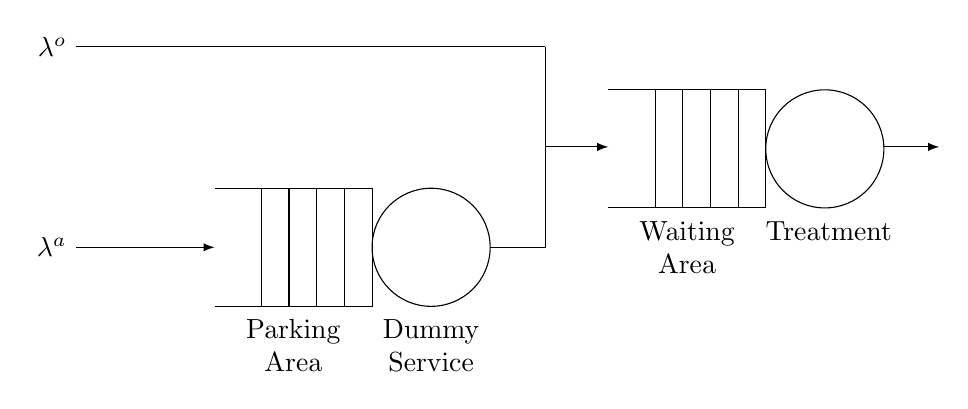
\begin{tikzpicture}[>=latex]
        % the rectangle with vertical rules (Queue 1)
        \draw (0,0) -- ++(2cm,0) -- ++(0,-1.5cm) -- ++(-2cm,0);
        \foreach \i in {1,...,4}
        \draw (2cm-\i*10pt,0) -- +(0,-1.5cm);
        
        % the circle (Queue 1)
        \draw (2.75,-0.75cm) circle [radius=0.75cm];

        % the rectangle with vertical rules (Queue 2)
        \draw (5,1.25) -- ++(2cm,0) -- ++(0,-1.5cm) -- ++(-2cm,0);
        \foreach \i in {1,...,4}
        \draw (7cm-\i*10pt,1.25) -- +(0,-1.5cm);

        % the circle (Queue 2)
        \draw (7.75,0.5) circle [radius=0.75cm];

        % the arrows and labels (Queue 1+2)
        \draw[-] (3.5,-0.75) -- +(20pt,0);
        \draw[<-] (0,-0.75) -- +(-50pt,0) node[left] {\( \lambda^a \)};
        \draw[->] (8.5,0.525) -- +(20pt,0);
        \node[align=center] at (1cm,-2cm) {Parking \\ Area};
        \node[align=center] at (2.75cm,-2cm) {Dummy \\ Service};
        \node[align=center] at (6cm,-0.75cm) {Waiting \\ Area};
        \node[align=center] at (7.8cm,-0.75cm) {Treatment \\ };
        
        \draw (4.2, 1.8) -- +(-169.5pt,0) node[left] {\( \lambda^o \)};
        \draw (4.2, 1.8) -- (4.2, -0.75);
        \draw[->] (4.2, 0.525) -- (5, 0.525);

    \end{tikzpicture}
\end{figure}


\begin{figure}
    \centering
    \begin{tikzpicture}[-, node distance = 1cm, auto, every node/.style={scale=0.5}]

        % Variables
        \tikzmath{
            let \altdist = 1.5cm;
            let \minsz = 1.5cm;
        }

        % First Line
        \node[state, minimum size=1.5cm] (zero) {(0,0)};
        \node[state, minimum size=1.5cm,  right=of zero] (one) {(0,1)};
        \node[draw=none, minimum size=1.5cm, right=of one] (two) {\dots};
        \node[state, minimum size=1.5cm, right=of two] (three) {(0,T)};
        \node[state, node distance = \altdist, minimum size=\minsz, right=of three] (four) {(0,T+1)};
        \node[draw=none, node distance = \altdist, minimum size=\minsz, right=of four] (five) {\dots};
        \node[state, node distance = \altdist, minimum size=\minsz, right=of five] (six) {(0,C)};
        \node[draw=none, minimum size=\minsz, right=of six] (seven) {\dots};

        % Second Line
        \node[state, minimum size=\minsz, below=of three] (three_one) {(1,T)};
        \node[state, minimum size=\minsz, below=of four] (four_one) {(1,T+1)};
        \node[draw=none, minimum size=\minsz, below=of five] (five_one) {\dots};
        \node[state, node distance = \altdist, minimum size=\minsz, right=of five_one] (six_one) {(1,C)};
        \node[draw=none, minimum size=\minsz, right=of six_one] (seven_one) {\dots};

        % Third Line
        \node[state, minimum size=\minsz, below=of three_one] (three_two) {(2,T)};
        \node[state, minimum size=\minsz, below=of four_one] (four_two) {(2,T+1)};
        \node[draw=none, minimum size=\minsz, below=of five_one] (five_two) {\dots};
        \node[state, node distance = \altdist, minimum size=\minsz, right=of five_two] (six_two) {(2,C)};
        \node[draw=none, minimum size=\minsz, right=of six_two] (seven_two) {\dots};

        % Fourth line
        \node[draw=none, minimum size=\minsz, below=of three_two] (three_three) {\vdots};
        \node[draw=none, minimum size=\minsz, below=of four_two] (four_three) {\vdots};
        \node[draw=none, minimum size=\minsz, below=of five_two] (five_three) {};
        \node[draw=none, node distance = \altdist, minimum size=\minsz, right=of five_three] (six_three) {\vdots};

        \draw[every loop]
            % First Horizontal Edges
            (zero) edge[bend left] node {\( \Lambda \)} (one)
            (one) edge[bend left] node [above] {\( \mu \)} (zero)
            (one) edge[bend left] node {\( \Lambda \)} (two)
            (two) edge[bend left] node [above] {\( 2 \mu \)} (one)
            (two) edge[bend left] node {\( \Lambda \)} (three)
            (three) edge[bend left] node [above] {\( T \mu \)} (two)
            (three) edge[bend left] node {\( \lambda^o \)} (four)
            (four) edge[bend left] node [above] {\( (T+1) \mu \)} (three)
            (four) edge[bend left] node {\( \lambda^o \)} (five)
            (five) edge[bend left] node [above] {\( (T+2) \mu \)} (four)
            (five) edge[bend left] node {\( \lambda^o \)} (six)
            (six) edge[bend left] node [above] {\( C\mu \)} (five)
            (six) edge[bend left] node {\( \lambda^o \)} (seven)
            (seven) edge[bend left] node [above] {\( C\mu \)} (six)

            % Second Horizontal Edges
            (three_one) edge[bend left] node {\( \lambda^o \)} (four_one)
            (four_one) edge[bend left] node [above] {\( (T+1) \mu \)} (three_one)
            (four_one) edge[bend left] node {\( \lambda^o \)} (five_one)
            (five_one) edge[bend left] node [above] {\( (T+2) \mu \)} (four_one)
            (five_one) edge[bend left] node {\( \lambda^o \)} (six_one)
            (six_one) edge[bend left] node [above] {\( C\mu \)} (five_one)
            (six_one) edge[bend left] node {\( \lambda^o \)} (seven_one)
            (seven_one) edge[bend left] node [above] {\( C\mu \)} (six_one)

            % Third Horizontal Edges
            (three_two) edge[bend left] node {\( \lambda^o \)} (four_two)
            (four_two) edge[bend left] node [above] {\( (T+1) \mu \)} (three_two)
            (four_two) edge[bend left] node {\( \lambda^o \)} (five_two)
            (five_two) edge[bend left] node [above] {\( (T+2) \mu \)} (four_two)
            (five_two) edge[bend left] node {\( \lambda^o \)} (six_two)
            (six_two) edge[bend left] node [above] {\( C\mu \)} (five_two)
            (six_two) edge[bend left] node {\( \lambda^o \)} (seven_two)
            (seven_two) edge[bend left] node [above] {\( C\mu \)} (six_two)

            % First Vertical Edges
            (three) edge[bend left] node {\( \lambda^A \)} (three_one)
            (three_one) edge[bend left] node {\( T \mu \)} (three)
            (three_one) edge[bend left] node {\( \lambda^A \)} (three_two)
            (three_two) edge[bend left] node {\( T\mu \)} (three_one)
            (three_two) edge[bend left] node {\( \lambda^A \)} (three_three)
            (three_three) edge[bend left] node {\( T\mu \)} (three_two)

            % Second Vertical Edges
            (four) edge node {\( \lambda^A \)} (four_one)
            (four_one) edge node {\( \lambda^A \)} (four_two)
            (four_two) edge node {\( \lambda^A \)} (four_three)

            %Third Vertical Edges
            (six) edge node {\( \lambda^A \)} (six_one)
            (six_one) edge node {\( \lambda^A \)} (six_two)
            (six_two) edge node {\( \lambda^A \)} (six_three)
            ;       
    \end{tikzpicture}
    \caption{Markov chains} 
    \label{Markov_2}
\end{figure}



\begin{figure}
    \centering
    \begin{tikzpicture}[-, node distance = 1cm, auto, every node/.style={scale=0.4}]

        % Variables
        \tikzmath{
            let \altdist = 1cm;
            let \minsz = 1.5cm;
        }

        % First Line
        \node[state, minimum size=1.5cm] (zero) {(0,0)};
        \node[state, minimum size=1.5cm,  right=of zero] (one) {(0,1)};
        \node[draw=none, minimum size=1.5cm, right=of one] (two) {\dots};
        \node[state, minimum size=1.5cm, right=of two] (three) {(0,T)};
        \node[state, node distance = \altdist, minimum size=\minsz, right=of three] (four) {(0,T+1)};
        \node[draw=none, minimum size=\minsz, right=of four] (five) {\dots};
        \node[draw=none, minimum size=\minsz, right=of five] (six) {\vdots};
        \node[draw=none, minimum size=\minsz, right=of six] (seven) {\dots};
        \node[state, minimum size=\minsz, right=of seven] (eight) {(0,C)};
        \node[draw=none, minimum size=\minsz, right=of eight] (nine) {\dots};


        % Second Line
        \node[state, minimum size=\minsz, below=of three] (three_one) {(1,T)};
        \node[state, minimum size=\minsz, below=of four] (four_one) {(1,T+1)};
        \node[draw=none, minimum size=\minsz, below=of five] (five_one) {\dots};
        \node[state, node distance = \altdist, minimum size=\minsz, right=of five_one] (six_one) {\( (u_i, v_i) \)};
        \node[draw=none, minimum size=\minsz, right=of six_one] (seven_one) {\dots};
        \node[state, node distance = \altdist, minimum size=\minsz, right=of seven_one] (eight_one) {(1,C)};
        \node[draw=none, minimum size=\minsz, right=of eight_one] (nine_one) {\dots};
        

        % Third Line
        \node[state, minimum size=\minsz, below=of three_one] (three_two) {(2,T)};
        \node[state, minimum size=\minsz, below=of four_one] (four_two) {(2,T+1)};
        \node[draw=none, minimum size=\minsz, below=of five_one] (five_two) {\dots};
        \node[draw=none, node distance = \altdist, minimum size=\minsz, right=of five_two] (six_two) {\vdots};
        \node[draw=none, minimum size=\minsz, right=of six_two] (seven_two) {\dots};
        \node[state, node distance = \altdist, minimum size=\minsz, right=of seven_two] (eight_two) {(2,C)};
        \node[draw=none, minimum size=\minsz, right=of eight_two] (nine_two) {\dots};

        % Fourth line
        \node[draw=none, minimum size=\minsz, below=of three_two] (three_three) {\vdots};
        \node[draw=none, minimum size=\minsz, below=of four_two] (four_three) {\vdots};
        \node[draw=none, minimum size=\minsz, below=of five_two] (five_three) {};
        \node[draw=none, node distance = \altdist, minimum size=\minsz, right=of five_three] (six_three) {};
        \node[draw=none, node distance = \altdist, minimum size=\minsz, below=of eight_two] (eight_three) {\vdots};


        \draw[every loop]
            % First Horizontal Edges
            (zero) edge[bend left] node {\( \Lambda \)} (one)
            (one) edge[bend left] node {\( \mu \)} (zero)
            (one) edge[bend left] node {\( \Lambda \)} (two)
            (two) edge[bend left] node {\( 2 \mu \)} (one)
            (two) edge[bend left] node {\( \Lambda \)} (three)
            (three) edge[bend left] node {\( T \mu \)} (two)
            (three) edge[bend left] node {\( \lambda^o \)} (four)
            (four) edge[bend left] node {\( (T+1) \mu \)} (three)
            (four) edge[bend left] node {\( \lambda^o \)} (five)
            (five) edge[bend left] node {\( (T+2) \mu \)} (four)
            % (five) edge[bend left] node {\( \lambda^o \)} (six)
            % (six) edge[bend left] node [above] {\( C\mu \)} (five)
            % (six) edge[bend left] node {\( \lambda^o \)} (seven)
            % (seven) edge[bend left] node [above] {\( C\mu \)} (six)
            (seven) edge[bend left] node {\( \lambda^o \)} (eight)
            (eight) edge[bend left] node {\( C\mu \)} (seven)
            (eight) edge[bend left] node {\( \lambda^o \)} (nine)
            (nine) edge[bend left] node {\( C\mu \)} (eight)

            % Second Horizontal Edges
            (three_one) edge[bend left] node {\(\lambda^o\)} (four_one)
            (four_one) edge[bend left] node {\( (T+1) \mu \)} (three_one)
            (four_one) edge[bend left] node {\( \lambda^o \)} (five_one)
            (five_one) edge[bend left] node {\( (T+2) \mu \)} (four_one)
            (five_one) edge[bend left] node {\( \lambda^o \)} (six_one)
            (six_one) edge[bend left] node {\( v_i\mu \)} (five_one)
            (six_one) edge[bend left] node {\( \lambda^o \)} (seven_one)
            (seven_one) edge[bend left] node {\( (v_i+1)\mu \)} (six_one)
            (seven_one) edge[bend left] node {\( \lambda^o \)} (eight_one)
            (eight_one) edge[bend left] node {\( C\mu \)} (seven_one)
            (eight_one) edge[bend left] node {\( \lambda^o \)} (nine_one)
            (nine_one) edge[bend left] node {\( C\mu \)} (eight_one)

            % Third Horizontal Edges
            (three_two) edge[bend left] node {\( \lambda^o \)} (four_two)
            (four_two) edge[bend left] node {\( (T+1) \mu \)} (three_two)
            (four_two) edge[bend left] node {\( \lambda^o \)} (five_two)
            (five_two) edge[bend left] node {\( (T+2) \mu \)} (four_two)
            % (five_two) edge[bend left] node {\( \lambda^o \)} (six_two)
            % (six_two) edge[bend left] node [above] {\( C\mu \)} (five_two)
            % (six_two) edge[bend left] node {\( \lambda^o \)} (seven_two)
            % (seven_two) edge[bend left] node [above] {\( C\mu \)} (six_two)
            (seven_two) edge[bend left] node {\( \lambda^o \)} (eight_two)
            (eight_two) edge[bend left] node {\( C\mu \)} (seven_two)
            (eight_two) edge[bend left] node {\( \lambda^o \)} (nine_two)
            (nine_two) edge[bend left] node {\( C\mu \)} (eight_two)

            % First Vertical Edges
            (three) edge[bend left] node {\( \lambda^A \)} (three_one)
            (three_one) edge[bend left] node {\( T \mu \)} (three)
            (three_one) edge[bend left] node {\( \lambda^A \)} (three_two)
            (three_two) edge[bend left] node {\( T\mu \)} (three_one)
            (three_two) edge[bend left] node {\( \lambda^A \)} (three_three)
            (three_three) edge[bend left] node {\( T\mu \)} (three_two)

            % Second Vertical Edges
            (four) edge node {\( \lambda^A \)} (four_one)
            (four_one) edge node {\( \lambda^A \)} (four_two)
            (four_two) edge node {\( \lambda^A \)} (four_three)

            % Third Vertical Edges
            (six) edge node {\( \lambda^A \)} (six_one)
            (six_one) edge node {\( \lambda^A \)} (six_two)
            % (six_two) edge node {\( \lambda^A \)} (six_three)

            % Fourth Vertical Edges
            (eight) edge node {\( \lambda^A \)} (eight_one)
            (eight_one) edge node {\( \lambda^A \)} (eight_two)
            (eight_two) edge node {\( \lambda^A \)} (eight_three)
            ;       
    \end{tikzpicture}
    \caption{Markov chains} 
    \label{Markov_3}
\end{figure}


\begin{figure}
    \centering
    \begin{tikzpicture}[-, node distance = 0.9cm, auto, every node/.style={scale=0.5}]

        % Variables
        \tikzmath{
            let \initdist = 0.5cm;
            let \altdist = 1.2cm;
            let \minsz = 1.6cm;
            let \leftOne = -0.8;
            let \rightOne = 2.2;
            let \upOne = 0.8;
            let \downOne = -2.2;
            let \leftTwo = 2.25;
            let \rightTwo = 14.2;
            let \upTwo = -2.35;
            let \downTwo = -8.8;
        }

        % % Rectangle for S1
        % \draw[ultra thin, dashed] (\leftOne, \downOne) -- (\leftOne, \upOne);
        % \draw[ultra thin, dashed] (\leftOne, \upOne) -- (\rightOne, \upOne);
        % \draw[ultra thin, dashed] (\rightOne, \upOne) -- node {\Huge{\( \quad S_1 \)}}(\rightOne, \downOne);
        % \draw[ultra thin, dashed] (\rightOne, \downOne) -- (\leftOne, \downOne);

        % % Rectangle for S2
        % \draw[ultra thin, dashed] (\leftTwo, \downTwo) -- node {\Huge{\( S_2 \quad \)}}(\leftTwo, \upTwo);
        % \draw[ultra thin, dashed] (\leftTwo, \upTwo) -- (\rightTwo, \upTwo);
        % \draw[ultra thin, dashed] (\rightTwo, \upTwo) -- (\rightTwo, \downTwo);
        % \draw[ultra thin, dashed] (\rightTwo, \downTwo) -- (\leftTwo, \downTwo);

        % First Line
        \node[state, minimum size=1.5cm] (zero) {(0,0)};
        \node[state, node distance = \initdist, minimum size=\minsz, below right=of zero] (one) {(0,1)};
        \node[draw=none, node distance = \initdist, minimum size=\minsz, below right=of one] (two) {\textbf{\( \ddots \)}};
        \node[state, node distance = \initdist, minimum size=\minsz, below right=of two] (three) {(0,T)};
        \node[state, node distance = \altdist, minimum size=\minsz, right=of three] (four) {(0,T+1)};
        \node[draw=none, node distance = \altdist, minimum size=\minsz, right=of four] (five) {\textbf{\dots}};
        \node[draw=none, minimum size=\minsz, right=of five] (six) {\textbf{\vdots}};
        \node[draw=none, minimum size=\minsz, right=of six] (seven) {\textbf{\dots}};
        \node[state, minimum size=\minsz, right=of seven] (eight) {(0,C)};
        \node[draw=none, minimum size=\minsz, right=of eight] (nine) {\textbf{\dots}};


        % Second Line
        \node[state, minimum size=\minsz, below=of three] (three_one) {(1,T)};
        \node[state, minimum size=\minsz, below=of four] (four_one) {(1,T+1)};
        \node[draw=none, minimum size=\minsz, below=of five] (five_one) {\textbf{\dots}};
        \node[state, minimum size=\minsz, right=of five_one] (six_one) {\( (u_i, v_i) \)};
        \node[draw=none, minimum size=\minsz, right=of six_one] (seven_one) {\textbf{\dots}};
        \node[state, minimum size=\minsz, right=of seven_one] (eight_one) {(1,C)};
        \node[draw=none, minimum size=\minsz, right=of eight_one] (nine_one) {\textbf{\dots}};
        

        % Third Line
        \node[state, minimum size=\minsz, below=of three_one] (three_two) {(2,T)};
        \node[state, minimum size=\minsz, below=of four_one] (four_two) {(2,T+1)};
        \node[draw=none, minimum size=\minsz, below=of five_one] (five_two) {\textbf{\dots}};
        \node[draw=none, minimum size=\minsz, right=of five_two] (six_two) {\textbf{\vdots}};
        \node[draw=none, minimum size=\minsz, right=of six_two] (seven_two) {\textbf{\dots}};
        \node[state, minimum size=\minsz, right=of seven_two] (eight_two) {(2,C)};
        \node[draw=none, minimum size=\minsz, right=of eight_two] (nine_two) {\textbf{\dots}};

        % Fourth line
        \node[draw=none, node distance = \altdist, minimum size=\minsz, below=of three_two] (three_three) {\textbf{\vdots}};
        \node[draw=none, node distance = \altdist, minimum size=\minsz, below=of four_two] (four_three) {\textbf{\vdots}};
        \node[draw=none, node distance = \altdist, minimum size=\minsz, below=of five_two] (five_three) {};
        \node[draw=none, node distance = \altdist, minimum size=\minsz, below=of six_two] (six_three) {};
        \node[draw=none, node distance = \altdist, minimum size=\minsz, below=of eight_two] (eight_three) {\textbf{\vdots}};


        \draw[every loop]
            % First Horizontal Edges
            (zero) edge[bend left] node {\( \Lambda \)} (one)
            (one) edge[bend left] node {\( \mu \)} (zero)
            (one) edge[bend left] node {\( \Lambda \)} (two)
            (two) edge[bend left] node {\( 2 \mu \)} (one)
            (two) edge[bend left] node {\( \Lambda \)} (three)
            (three) edge[bend left] node {\( T \mu \)} (two)
            (three) edge[bend left] node {\( \lambda^o \)} (four)
            (four) edge[bend left] node {\( (T+1) \mu \)} (three)
            (four) edge[bend left] node {\( \lambda^o \)} (five)
            (five) edge[bend left] node {\( (T+2) \mu \)} (four)
            % (five) edge[bend left] node {\( \lambda^o \)} (six)
            % (six) edge[bend left] node [above] {\( C\mu \)} (five)
            % (six) edge[bend left] node {\( \lambda^o \)} (seven)
            % (seven) edge[bend left] node [above] {\( C\mu \)} (six)
            (seven) edge[bend left] node {\( \lambda^o \)} (eight)
            (eight) edge[bend left] node {\( C\mu \)} (seven)
            (eight) edge[bend left] node {\( \lambda^o \)} (nine)
            (nine) edge[bend left] node {\( C\mu \)} (eight)

            % Second Horizontal Edges
            (three_one) edge[bend left] node {\( \lambda^o \)} (four_one)
            (four_one) edge[bend left] node {\( (T+1) \mu \)} (three_one)
            (four_one) edge[bend left] node {\( \lambda^o \)} (five_one)
            (five_one) edge[bend left] node {\( (T+2) \mu \)} (four_one)
            (five_one) edge[bend left] node {\( \lambda^o \)} (six_one)
            (six_one) edge[bend left] node {\( v_i\mu \)} (five_one)
            (six_one) edge[bend left] node {\( \lambda^o \)} (seven_one)
            (seven_one) edge[bend left] node {\( (v_i+1)\mu \)} (six_one)
            (seven_one) edge[bend left] node {\( \lambda^o \)} (eight_one)
            (eight_one) edge[bend left] node {\( C\mu \)} (seven_one)
            (eight_one) edge[bend left] node {\( \lambda^o \)} (nine_one)
            (nine_one) edge[bend left] node {\( C\mu \)} (eight_one)

            % Third Horizontal Edges
            (three_two) edge[bend left] node {\( \lambda^o \)} (four_two)
            (four_two) edge[bend left] node [below] {\( (T+1) \mu \)} (three_two)
            (four_two) edge[bend left] node {\( \lambda^o \)} (five_two)
            (five_two) edge[bend left] node {\( (T+2) \mu \)} (four_two)
            % (five_two) edge[bend left] node {\( \lambda^o \)} (six_two)
            % (six_two) edge[bend left] node [above] {\( C\mu \)} (five_two)
            % (six_two) edge[bend left] node {\( \lambda^o \)} (seven_two)
            % (seven_two) edge[bend left] node [above] {\( C\mu \)} (six_two)
            (seven_two) edge[bend left] node {\( \lambda^o \)} (eight_two)
            (eight_two) edge[bend left] node {\( C\mu \)} (seven_two)
            (eight_two) edge[bend left] node {\( \lambda^o \)} (nine_two)
            (nine_two) edge[bend left] node {\( C\mu \)} (eight_two)

            % First Vertical Edges
            (three) edge[bend left] node {\( \lambda^A \)} (three_one)
            (three_one) edge[bend left] node {\( T \mu \)} (three)
            (three_one) edge[bend left] node {\( \lambda^A \)} (three_two)
            (three_two) edge[bend left] node {\( T\mu \)} (three_one)
            (three_two) edge[bend left] node {\( \lambda^A \)} (three_three)
            (three_three) edge[bend left] node {\( T\mu \)} (three_two)

            % Second Vertical Edges
            (four) edge node {\( \lambda^A \)} (four_one)
            (four_one) edge node {\( \lambda^A \)} (four_two)
            (four_two) edge node {\( \lambda^A \)} (four_three)

            % Third Vertical Edges
            (six) edge node {\( \lambda^A \)} (six_one)
            (six_one) edge node {\( \lambda^A \)} (six_two)
            % (six_two) edge node {\( \lambda^A \)} (six_three)

            % Fourth Vertical Edges
            (eight) edge node {\( \lambda^A \)} (eight_one)
            (eight_one) edge node {\( \lambda^A \)} (eight_two)
            (eight_two) edge node {\( \lambda^A \)} (eight_three)
            ;       
    \end{tikzpicture}
    \caption{Markov chains} 
    \label{Markov_4}
\end{figure}




\begin{figure}
    \centering
    \begin{tikzpicture}[-, node distance = 0.9cm, auto, every node/.style={scale=0.7}]

        % Markov chain variables
        \tikzmath{
            let \initdist = 0.5cm;
            let \altdist = 1.2cm;
            let \minsz = 1.6cm;
        }

        % S_1 and S_2 rectangles
        \tikzmath{
            let \leftOne = -0.8;
            let \rightOne = 2.7;
            let \upOne = 0.8;
            let \downOne = -2.7;
            let \leftTwo = 2.8;
            let \rightTwo = 13;
            let \upTwo = -2.95;
            let \downTwo = -16.4;
        }

        % General case variables
        \tikzmath{
            let \GCsmallx = 8.3;
            let \GCsmally = -9.5;
            let \GCbigx = 4.1;
            let \GCbigy = -11.8;
        }

        % % Rectangle for S1
        % \draw[ultra thin, dashed] (\leftOne, \downOne) -- (\leftOne, \upOne);
        % \draw[ultra thin, dashed] (\leftOne, \upOne) -- (\rightOne, \upOne);
        % \draw[ultra thin, dashed] (\rightOne, \upOne) -- node {\Huge{\( \quad S_1 \)}}(\rightOne, \downOne);
        % \draw[ultra thin, dashed] (\rightOne, \downOne) -- (\leftOne, \downOne);

        % % Rectangle for S2
        % \draw[ultra thin, dashed] (\leftTwo, \downTwo) -- node {\Huge{\( S_2 \quad \)}}(\leftTwo, \upTwo);
        % \draw[ultra thin, dashed] (\leftTwo, \upTwo) -- (\rightTwo, \upTwo);
        % \draw[ultra thin, dashed] (\rightTwo, \upTwo) -- (\rightTwo, \downTwo);
        % \draw[ultra thin, dashed] (\rightTwo, \downTwo) -- (\leftTwo, \downTwo);

        % Small square of general case
        \draw [thick] (\GCsmallx, \GCsmally) -- node {} (\GCsmallx + 0.4, \GCsmally);
        \draw [thick] (\GCsmallx + 0.4, \GCsmally) -- node {} (\GCsmallx + 0.4, \GCsmally - 0.4);
        \draw [thick] (\GCsmallx + 0.4, \GCsmally - 0.4) -- node {} (\GCsmallx, \GCsmally - 0.4);
        \draw [thick] (\GCsmallx, \GCsmally - 0.4) -- node {} (\GCsmallx, \GCsmally);


        % Dashed lines to from small square to big one 
        \draw [ultra thin] (\GCsmallx, \GCsmally) -- node {} (\GCbigx, \GCbigy);
        \draw [ultra thin] (\GCsmallx + 0.4, \GCsmally) -- node {} (\GCbigx + 4, \GCbigy);
        \draw [ultra thin] (\GCsmallx, \GCsmally - 0.4) -- node {} (7, \GCbigy);
        \draw [ultra thin] (\GCsmallx + 0.4, \GCsmally - 0.4) -- node {} (\GCbigx + 4, \GCbigy - 4);
        
        % Big Square of general case
        \draw [ultra thick] (\GCbigx, \GCbigy) -- node {} (\GCbigx + 4, \GCbigy);
        \draw [ultra thick] (\GCbigx + 4, \GCbigy) -- node {} (\GCbigx + 4, \GCbigy - 4);
        \draw [ultra thick] (\GCbigx + 4, \GCbigy - 4) -- node {General Case} (\GCbigx, \GCbigy - 4);
        \draw [ultra thick] (\GCbigx, \GCbigy - 4) -- node {} (\GCbigx, \GCbigy);

        % First Line
        \node[state, minimum size=1.5cm] (zero) {(0,0)};
        \node[state, node distance = \initdist, minimum size=\minsz, below right=of zero] (one) {(0,1)};
        \node[draw=none, node distance = \initdist, minimum size=\minsz, below right=of one] (two) {\textbf{\( \ddots \)}};
        \node[state, node distance = \initdist, minimum size=\minsz, below right=of two] (three) {(0,T)};
        \node[state, node distance = \altdist, minimum size=\minsz, right=of three] (four) {(0,T+1)};
        \node[draw=none, node distance = \altdist, minimum size=\minsz, right=of four] (five) {\textbf{\dots}};
        \node[state, minimum size=\minsz, right=of five] (six) {(0,C)};
        \node[draw=none, minimum size=\minsz, right=of six] (seven) {\textbf{\dots}};

        % Second Line
        \node[state, minimum size=\minsz, below=of three] (three_one) {(1,T)};
        \node[state, minimum size=\minsz, below=of four] (four_one) {(1,T+1)};
        \node[draw=none, minimum size=\minsz, below=of five] (five_one) {\textbf{\dots}};
        \node[state, minimum size=\minsz, right=of five_one] (six_one) {(1,C)};
        \node[draw=none, minimum size=\minsz, right=of six_one] (seven_one) {\textbf{\dots}};
        
        % Third Line
        \node[state, minimum size=\minsz, below=of three_one] (three_two) {(2,T)};
        \node[state, minimum size=\minsz, below=of four_one] (four_two) {(2,T+1)};
        \node[draw=none, minimum size=\minsz, below=of five_one] (five_two) {\textbf{\dots}};
        \node[state, minimum size=\minsz, right=of five_two] (six_two) {(2,C)};
        \node[draw=none, minimum size=\minsz, right=of six_two] (seven_two) {\textbf{\dots}};

        % Fourth line
        \node[draw=none, node distance = \altdist, minimum size=\minsz, below=of three_two] (three_three) {\textbf{\vdots}};
        \node[draw=none, node distance = \altdist, minimum size=\minsz, below=of four_two] (four_three) {\textbf{\vdots}};
        \node[draw=none, node distance = 2cm, minimum size=\minsz, below=of five_two] (five_three) {};
        \node[draw=none, node distance = \altdist, minimum size=\minsz, below=of six_two] (six_three) {\textbf{\vdots}};

        % Fifth line
        % \node[state, node distance = \altdist, minimum size=\minsz, below=of five_three] (general_case_mid) {\( (u_i, v_i) \)};
        \node[draw=none, node distance = 0.3cm, minimum size=\minsz, below=of four_three] (general_case_up) {};
        \node[state, node distance = \altdist, minimum size=\minsz, below=of general_case_up] (general_case_mid) {\( (u_i, v_i) \)};

        \node[draw=none, node distance = \altdist, minimum size=\minsz, below=of general_case_mid] (general_case_down) {};
        \node[draw=none, node distance = \altdist, minimum size=\minsz, left=of general_case_mid] (general_case_left) {};
        \node[draw=none, node distance = \altdist, minimum size=\minsz, right=of general_case_mid] (general_case_right) {};

        \draw[every loop]
            % First Horizontal Edges
            (zero) edge[bend left] node {\( \Lambda \)} (one)
            (one) edge[bend left] node {\( \mu \)} (zero)
            (one) edge[bend left] node {\( \Lambda \)} (two)
            (two) edge[bend left] node {\( 2 \mu \)} (one)
            (two) edge[bend left] node {\( \Lambda \)} (three)
            (three) edge[bend left] node {\( T \mu \)} (two)
            (three) edge[bend left] node {\( \lambda^o \)} (four)
            (four) edge[bend left] node {\( (T+1) \mu \)} (three)
            (four) edge[bend left] node {\( \lambda^o \)} (five)
            (five) edge[bend left] node {\( (T+2) \mu \)} (four)
            (five) edge[bend left] node {\( \lambda^o \)} (six)
            (six) edge[bend left] node {\( C\mu \)} (five)
            (six) edge[bend left] node {\( \lambda^o \)} (seven)
            (seven) edge[bend left] node {\( C\mu \)} (six)

            % Second Horizontal Edges
            (three_one) edge[bend left] node {\( \lambda^o \)} (four_one)
            (four_one) edge[bend left] node {\( (T+1) \mu \)} (three_one)
            (four_one) edge[bend left] node {\( \lambda^o \)} (five_one)
            (five_one) edge[bend left] node {\( (T+2) \mu \)} (four_one)
            (five_one) edge[bend left] node {\( \lambda^o \)} (six_one)
            (six_one) edge[bend left] node {\( C\mu \)} (five_one)
            (six_one) edge[bend left] node {\( \lambda^o \)} (seven_one)
            (seven_one) edge[bend left] node {\( C\mu \)} (six_one)

            % Third Horizontal Edges
            (three_two) edge[bend left] node {\( \lambda^o \)} (four_two)
            (four_two) edge[bend left] node [below] {\( (T+1) \mu \)} (three_two)
            (four_two) edge[bend left] node {\( \lambda^o \)} (five_two)
            (five_two) edge[bend left] node {\( (T+2) \mu \)} (four_two)
            (five_two) edge[bend left] node {\( \lambda^o \)} (six_two)
            (six_two) edge[bend left] node {\( C\mu \)} (five_two)
            (six_two) edge[bend left] node {\( \lambda^o \)} (seven_two)
            (seven_two) edge[bend left] node {\( C\mu \)} (six_two)

            % First Vertical Edges
            (three) edge[bend left] node {\( \lambda^A \)} (three_one)
            (three_one) edge[bend left] node {\( T \mu \)} (three)
            (three_one) edge[bend left] node {\( \lambda^A \)} (three_two)
            (three_two) edge[bend left] node {\( T\mu \)} (three_one)
            (three_two) edge[bend left] node {\( \lambda^A \)} (three_three)
            (three_three) edge[bend left] node {\( T\mu \)} (three_two)

            % Second Vertical Edges
            (four) edge node {\( \lambda^A \)} (four_one)
            (four_one) edge node {\( \lambda^A \)} (four_two)
            (four_two) edge node {\( \lambda^A \)} (four_three)

            % Fourth Vertical Edges
            (six) edge node {\( \lambda^A \)} (six_one)
            (six_one) edge node {\( \lambda^A \)} (six_two)
            (six_two) edge node {\( \lambda^A \)} (six_three)

            % General Case
            (general_case_left) edge[bend left] node {\( \lambda^o \)} (general_case_mid)
            (general_case_mid) edge[bend left] node {\( v_i \mu \)} (general_case_left)
            (general_case_right) edge[bend left] node {\( (v_i +1) \mu \)} (general_case_mid)
            (general_case_mid) edge[bend left] node {\( \lambda_o \)} (general_case_right)
            % (five_three) edge node {\( \lambda_A \)} (general_case_mid)
            (general_case_up) edge node {\( \lambda_A \)} (general_case_mid)
            (general_case_mid) edge node {\( \lambda_A \)} (general_case_down)
            ;
    \end{tikzpicture}
    \caption{Markov chain} 
    \label{Markov_5}
\end{figure}


\end{figure}

\begin{multicols}{4}
    \begin{figure}[H]
        \centering
        \scalebox{0.6}{
            

\begin{tikzpicture}[-, node distance = 1cm, auto]
\node[state] (u0v0) {(0,0)};
\node[state, right=of u0v0] (u0v1) {(0,1)};
\draw[->](u0v1) edge node {\(\mu \)} (u0v0);
\node[state, below=of u0v1] (u1v1) {(1,1)};
\draw[->](u1v1) edge node {\(\mu \)} (u0v1);
\node[state, right=of u0v1] (u0v2) {(0,2)};
\node[state, right=of u1v1] (u1v2) {(1,2)};
\draw[->](u1v2) edge node {\(\mu \)} (u1v1);
\node[state, right=of u0v2] (u0v3) {(0,3)};
\node[state, right=of u1v2] (u1v3) {(1,3)};
\draw[->](u1v3) edge node {\(\mu \)} (u1v2);
\draw[->](u0v2) edge node {\(\lambda_2 \)} (u1v2);
\draw[->](u0v3) edge node {\(\lambda_2 \)} (u1v3);
\end{tikzpicture}}
    \end{figure}
    \vspace*{\fill}
    \columnbreak
    \vspace*{0cm}
    \begin{equation*}
        (\lambda_2)^2 \mu^4
    \end{equation*}
    \vspace*{\fill}
    \columnbreak
    \begin{figure}[H]
        \centering
        \scalebox{0.6}{
            

\begin{tikzpicture}[-, node distance = 1cm, auto]
\node[state] (u0v0) {(0,0)};
\node[state, right=of u0v0] (u0v1) {(0,1)};
\draw[->](u0v1) edge node {\(\mu \)} (u0v0);
\node[state, below=of u0v1] (u1v1) {(1,1)};
\draw[->](u1v1) edge node {\(\mu \)} (u0v1);
\node[state, right=of u0v1] (u0v2) {(0,2)};
\node[state, right=of u1v1] (u1v2) {(1,2)};
\draw[->](u1v2) edge node {\(\mu \)} (u1v1);
\node[state, right=of u0v2] (u0v3) {(0,3)};
\node[state, right=of u1v2] (u1v3) {(1,3)};
\draw[->](u1v3) edge node {\(\mu \)} (u1v2);
\draw[->](u0v2) edge node {\(\mu \)} (u0v1);
\draw[->](u0v3) edge node {\(\lambda_2 \)} (u1v3);
\end{tikzpicture}}
    \end{figure}
    \vspace*{\fill}
    \columnbreak
    \vspace*{0.3cm}
    \begin{equation*}
        \lambda_2 \mu^5
    \end{equation*}
\end{multicols}

\begin{multicols}{4}
    \begin{figure}[H]
        \centering
        \scalebox{0.6}{
            

\begin{tikzpicture}[-, node distance = 1cm, auto]
\node[state] (u0v0) {(0,0)};
\node[state, right=of u0v0] (u0v1) {(0,1)};
\draw[->](u0v1) edge node {\(\mu \)} (u0v0);
\node[state, below=of u0v1] (u1v1) {(1,1)};
\draw[->](u1v1) edge node {\(\mu \)} (u0v1);
\node[state, right=of u0v1] (u0v2) {(0,2)};
\node[state, right=of u1v1] (u1v2) {(1,2)};
\draw[->](u1v2) edge node {\(\mu \)} (u1v1);
\node[state, right=of u0v2] (u0v3) {(0,3)};
\node[state, right=of u1v2] (u1v3) {(1,3)};
\draw[->](u1v3) edge node {\(\mu \)} (u1v2);
\draw[->](u0v2) edge node {\(\lambda_2 \)} (u1v2);
\draw[->](u0v3) edge node {\(\mu \)} (u0v2);
\end{tikzpicture}}
    \end{figure}
    \vspace*{\fill}
    \columnbreak
    \vspace*{0.3cm}
    \begin{equation*}
        \lambda_2 \mu^5
    \end{equation*}
    \vspace*{\fill}
    \columnbreak
    \begin{figure}[H]
        \centering
        \scalebox{0.6}{
            

\begin{tikzpicture}[-, node distance = 1cm, auto]
\node[state] (u0v0) {(0,0)};
\node[state, right=of u0v0] (u0v1) {(0,1)};
\draw[->](u0v1) edge node {\(\mu \)} (u0v0);
\node[state, below=of u0v1] (u1v1) {(1,1)};
\draw[->](u1v1) edge node {\(\mu \)} (u0v1);
\node[state, right=of u0v1] (u0v2) {(0,2)};
\node[state, right=of u1v1] (u1v2) {(1,2)};
\draw[->](u1v2) edge node {\(\mu \)} (u1v1);
\node[state, right=of u0v2] (u0v3) {(0,3)};
\node[state, right=of u1v2] (u1v3) {(1,3)};
\draw[->](u1v3) edge node {\(\mu \)} (u1v2);
\draw[->](u0v2) edge node {\(\lambda_1 \)} (u0v3);
\draw[->](u0v3) edge node {\(\lambda_2 \)} (u1v3);
\end{tikzpicture}}
    \end{figure}
    \vspace*{\fill}
    \columnbreak
    \vspace*{0.3cm}
    \begin{equation*}
        \mu^6
    \end{equation*}
\end{multicols}


\begin{equation*}
    \tilde{\pi}_{(0,0)} = (\lambda_2)^2 \mu^4 + 2 \lambda_2 \mu^5 + \mu^6
\end{equation*}

\newpage
\subsubsection{Conjecture of adding rows}

Let us consider three Markov models with the same number of servers \(C=1\), 
the same threshold \(T=1\), the same service centre capacity \(N=2\) but 
\(M\in\{1, 2, 3\}\).


\begin{multicols}{3}
    \begin{figure}[H]
        \centering
        \scalebox{0.8}{
            \section{Figures that might be useful}
\begin{figure}[h]
    \centering
    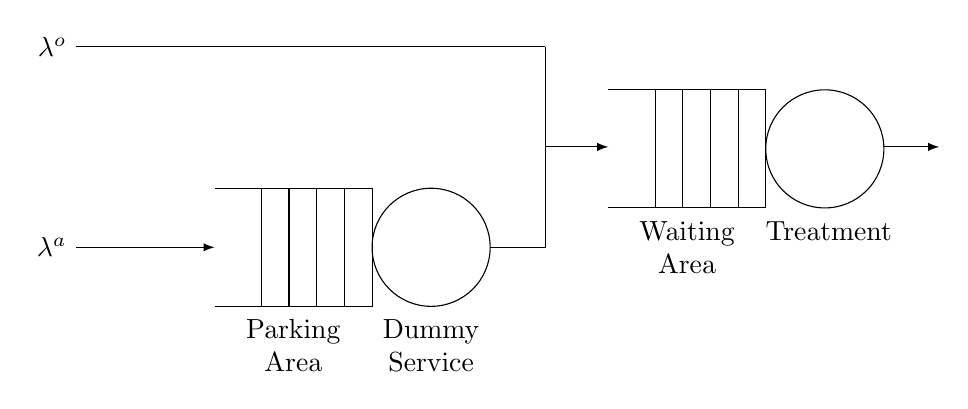
\begin{tikzpicture}[>=latex]
        % the rectangle with vertical rules (Queue 1)
        \draw (0,0) -- ++(2cm,0) -- ++(0,-1.5cm) -- ++(-2cm,0);
        \foreach \i in {1,...,4}
        \draw (2cm-\i*10pt,0) -- +(0,-1.5cm);
        
        % the circle (Queue 1)
        \draw (2.75,-0.75cm) circle [radius=0.75cm];

        % the rectangle with vertical rules (Queue 2)
        \draw (5,1.25) -- ++(2cm,0) -- ++(0,-1.5cm) -- ++(-2cm,0);
        \foreach \i in {1,...,4}
        \draw (7cm-\i*10pt,1.25) -- +(0,-1.5cm);

        % the circle (Queue 2)
        \draw (7.75,0.5) circle [radius=0.75cm];

        % the arrows and labels (Queue 1+2)
        \draw[-] (3.5,-0.75) -- +(20pt,0);
        \draw[<-] (0,-0.75) -- +(-50pt,0) node[left] {\( \lambda^a \)};
        \draw[->] (8.5,0.525) -- +(20pt,0);
        \node[align=center] at (1cm,-2cm) {Parking \\ Area};
        \node[align=center] at (2.75cm,-2cm) {Dummy \\ Service};
        \node[align=center] at (6cm,-0.75cm) {Waiting \\ Area};
        \node[align=center] at (7.8cm,-0.75cm) {Treatment \\ };
        
        \draw (4.2, 1.8) -- +(-169.5pt,0) node[left] {\( \lambda^o \)};
        \draw (4.2, 1.8) -- (4.2, -0.75);
        \draw[->] (4.2, 0.525) -- (5, 0.525);

    \end{tikzpicture}
\end{figure}


\begin{figure}
    \centering
    \begin{tikzpicture}[-, node distance = 1cm, auto, every node/.style={scale=0.5}]

        % Variables
        \tikzmath{
            let \altdist = 1.5cm;
            let \minsz = 1.5cm;
        }

        % First Line
        \node[state, minimum size=1.5cm] (zero) {(0,0)};
        \node[state, minimum size=1.5cm,  right=of zero] (one) {(0,1)};
        \node[draw=none, minimum size=1.5cm, right=of one] (two) {\dots};
        \node[state, minimum size=1.5cm, right=of two] (three) {(0,T)};
        \node[state, node distance = \altdist, minimum size=\minsz, right=of three] (four) {(0,T+1)};
        \node[draw=none, node distance = \altdist, minimum size=\minsz, right=of four] (five) {\dots};
        \node[state, node distance = \altdist, minimum size=\minsz, right=of five] (six) {(0,C)};
        \node[draw=none, minimum size=\minsz, right=of six] (seven) {\dots};

        % Second Line
        \node[state, minimum size=\minsz, below=of three] (three_one) {(1,T)};
        \node[state, minimum size=\minsz, below=of four] (four_one) {(1,T+1)};
        \node[draw=none, minimum size=\minsz, below=of five] (five_one) {\dots};
        \node[state, node distance = \altdist, minimum size=\minsz, right=of five_one] (six_one) {(1,C)};
        \node[draw=none, minimum size=\minsz, right=of six_one] (seven_one) {\dots};

        % Third Line
        \node[state, minimum size=\minsz, below=of three_one] (three_two) {(2,T)};
        \node[state, minimum size=\minsz, below=of four_one] (four_two) {(2,T+1)};
        \node[draw=none, minimum size=\minsz, below=of five_one] (five_two) {\dots};
        \node[state, node distance = \altdist, minimum size=\minsz, right=of five_two] (six_two) {(2,C)};
        \node[draw=none, minimum size=\minsz, right=of six_two] (seven_two) {\dots};

        % Fourth line
        \node[draw=none, minimum size=\minsz, below=of three_two] (three_three) {\vdots};
        \node[draw=none, minimum size=\minsz, below=of four_two] (four_three) {\vdots};
        \node[draw=none, minimum size=\minsz, below=of five_two] (five_three) {};
        \node[draw=none, node distance = \altdist, minimum size=\minsz, right=of five_three] (six_three) {\vdots};

        \draw[every loop]
            % First Horizontal Edges
            (zero) edge[bend left] node {\( \Lambda \)} (one)
            (one) edge[bend left] node [above] {\( \mu \)} (zero)
            (one) edge[bend left] node {\( \Lambda \)} (two)
            (two) edge[bend left] node [above] {\( 2 \mu \)} (one)
            (two) edge[bend left] node {\( \Lambda \)} (three)
            (three) edge[bend left] node [above] {\( T \mu \)} (two)
            (three) edge[bend left] node {\( \lambda^o \)} (four)
            (four) edge[bend left] node [above] {\( (T+1) \mu \)} (three)
            (four) edge[bend left] node {\( \lambda^o \)} (five)
            (five) edge[bend left] node [above] {\( (T+2) \mu \)} (four)
            (five) edge[bend left] node {\( \lambda^o \)} (six)
            (six) edge[bend left] node [above] {\( C\mu \)} (five)
            (six) edge[bend left] node {\( \lambda^o \)} (seven)
            (seven) edge[bend left] node [above] {\( C\mu \)} (six)

            % Second Horizontal Edges
            (three_one) edge[bend left] node {\( \lambda^o \)} (four_one)
            (four_one) edge[bend left] node [above] {\( (T+1) \mu \)} (three_one)
            (four_one) edge[bend left] node {\( \lambda^o \)} (five_one)
            (five_one) edge[bend left] node [above] {\( (T+2) \mu \)} (four_one)
            (five_one) edge[bend left] node {\( \lambda^o \)} (six_one)
            (six_one) edge[bend left] node [above] {\( C\mu \)} (five_one)
            (six_one) edge[bend left] node {\( \lambda^o \)} (seven_one)
            (seven_one) edge[bend left] node [above] {\( C\mu \)} (six_one)

            % Third Horizontal Edges
            (three_two) edge[bend left] node {\( \lambda^o \)} (four_two)
            (four_two) edge[bend left] node [above] {\( (T+1) \mu \)} (three_two)
            (four_two) edge[bend left] node {\( \lambda^o \)} (five_two)
            (five_two) edge[bend left] node [above] {\( (T+2) \mu \)} (four_two)
            (five_two) edge[bend left] node {\( \lambda^o \)} (six_two)
            (six_two) edge[bend left] node [above] {\( C\mu \)} (five_two)
            (six_two) edge[bend left] node {\( \lambda^o \)} (seven_two)
            (seven_two) edge[bend left] node [above] {\( C\mu \)} (six_two)

            % First Vertical Edges
            (three) edge[bend left] node {\( \lambda^A \)} (three_one)
            (three_one) edge[bend left] node {\( T \mu \)} (three)
            (three_one) edge[bend left] node {\( \lambda^A \)} (three_two)
            (three_two) edge[bend left] node {\( T\mu \)} (three_one)
            (three_two) edge[bend left] node {\( \lambda^A \)} (three_three)
            (three_three) edge[bend left] node {\( T\mu \)} (three_two)

            % Second Vertical Edges
            (four) edge node {\( \lambda^A \)} (four_one)
            (four_one) edge node {\( \lambda^A \)} (four_two)
            (four_two) edge node {\( \lambda^A \)} (four_three)

            %Third Vertical Edges
            (six) edge node {\( \lambda^A \)} (six_one)
            (six_one) edge node {\( \lambda^A \)} (six_two)
            (six_two) edge node {\( \lambda^A \)} (six_three)
            ;       
    \end{tikzpicture}
    \caption{Markov chains} 
    \label{Markov_2}
\end{figure}



\begin{figure}
    \centering
    \begin{tikzpicture}[-, node distance = 1cm, auto, every node/.style={scale=0.4}]

        % Variables
        \tikzmath{
            let \altdist = 1cm;
            let \minsz = 1.5cm;
        }

        % First Line
        \node[state, minimum size=1.5cm] (zero) {(0,0)};
        \node[state, minimum size=1.5cm,  right=of zero] (one) {(0,1)};
        \node[draw=none, minimum size=1.5cm, right=of one] (two) {\dots};
        \node[state, minimum size=1.5cm, right=of two] (three) {(0,T)};
        \node[state, node distance = \altdist, minimum size=\minsz, right=of three] (four) {(0,T+1)};
        \node[draw=none, minimum size=\minsz, right=of four] (five) {\dots};
        \node[draw=none, minimum size=\minsz, right=of five] (six) {\vdots};
        \node[draw=none, minimum size=\minsz, right=of six] (seven) {\dots};
        \node[state, minimum size=\minsz, right=of seven] (eight) {(0,C)};
        \node[draw=none, minimum size=\minsz, right=of eight] (nine) {\dots};


        % Second Line
        \node[state, minimum size=\minsz, below=of three] (three_one) {(1,T)};
        \node[state, minimum size=\minsz, below=of four] (four_one) {(1,T+1)};
        \node[draw=none, minimum size=\minsz, below=of five] (five_one) {\dots};
        \node[state, node distance = \altdist, minimum size=\minsz, right=of five_one] (six_one) {\( (u_i, v_i) \)};
        \node[draw=none, minimum size=\minsz, right=of six_one] (seven_one) {\dots};
        \node[state, node distance = \altdist, minimum size=\minsz, right=of seven_one] (eight_one) {(1,C)};
        \node[draw=none, minimum size=\minsz, right=of eight_one] (nine_one) {\dots};
        

        % Third Line
        \node[state, minimum size=\minsz, below=of three_one] (three_two) {(2,T)};
        \node[state, minimum size=\minsz, below=of four_one] (four_two) {(2,T+1)};
        \node[draw=none, minimum size=\minsz, below=of five_one] (five_two) {\dots};
        \node[draw=none, node distance = \altdist, minimum size=\minsz, right=of five_two] (six_two) {\vdots};
        \node[draw=none, minimum size=\minsz, right=of six_two] (seven_two) {\dots};
        \node[state, node distance = \altdist, minimum size=\minsz, right=of seven_two] (eight_two) {(2,C)};
        \node[draw=none, minimum size=\minsz, right=of eight_two] (nine_two) {\dots};

        % Fourth line
        \node[draw=none, minimum size=\minsz, below=of three_two] (three_three) {\vdots};
        \node[draw=none, minimum size=\minsz, below=of four_two] (four_three) {\vdots};
        \node[draw=none, minimum size=\minsz, below=of five_two] (five_three) {};
        \node[draw=none, node distance = \altdist, minimum size=\minsz, right=of five_three] (six_three) {};
        \node[draw=none, node distance = \altdist, minimum size=\minsz, below=of eight_two] (eight_three) {\vdots};


        \draw[every loop]
            % First Horizontal Edges
            (zero) edge[bend left] node {\( \Lambda \)} (one)
            (one) edge[bend left] node {\( \mu \)} (zero)
            (one) edge[bend left] node {\( \Lambda \)} (two)
            (two) edge[bend left] node {\( 2 \mu \)} (one)
            (two) edge[bend left] node {\( \Lambda \)} (three)
            (three) edge[bend left] node {\( T \mu \)} (two)
            (three) edge[bend left] node {\( \lambda^o \)} (four)
            (four) edge[bend left] node {\( (T+1) \mu \)} (three)
            (four) edge[bend left] node {\( \lambda^o \)} (five)
            (five) edge[bend left] node {\( (T+2) \mu \)} (four)
            % (five) edge[bend left] node {\( \lambda^o \)} (six)
            % (six) edge[bend left] node [above] {\( C\mu \)} (five)
            % (six) edge[bend left] node {\( \lambda^o \)} (seven)
            % (seven) edge[bend left] node [above] {\( C\mu \)} (six)
            (seven) edge[bend left] node {\( \lambda^o \)} (eight)
            (eight) edge[bend left] node {\( C\mu \)} (seven)
            (eight) edge[bend left] node {\( \lambda^o \)} (nine)
            (nine) edge[bend left] node {\( C\mu \)} (eight)

            % Second Horizontal Edges
            (three_one) edge[bend left] node {\(\lambda^o\)} (four_one)
            (four_one) edge[bend left] node {\( (T+1) \mu \)} (three_one)
            (four_one) edge[bend left] node {\( \lambda^o \)} (five_one)
            (five_one) edge[bend left] node {\( (T+2) \mu \)} (four_one)
            (five_one) edge[bend left] node {\( \lambda^o \)} (six_one)
            (six_one) edge[bend left] node {\( v_i\mu \)} (five_one)
            (six_one) edge[bend left] node {\( \lambda^o \)} (seven_one)
            (seven_one) edge[bend left] node {\( (v_i+1)\mu \)} (six_one)
            (seven_one) edge[bend left] node {\( \lambda^o \)} (eight_one)
            (eight_one) edge[bend left] node {\( C\mu \)} (seven_one)
            (eight_one) edge[bend left] node {\( \lambda^o \)} (nine_one)
            (nine_one) edge[bend left] node {\( C\mu \)} (eight_one)

            % Third Horizontal Edges
            (three_two) edge[bend left] node {\( \lambda^o \)} (four_two)
            (four_two) edge[bend left] node {\( (T+1) \mu \)} (three_two)
            (four_two) edge[bend left] node {\( \lambda^o \)} (five_two)
            (five_two) edge[bend left] node {\( (T+2) \mu \)} (four_two)
            % (five_two) edge[bend left] node {\( \lambda^o \)} (six_two)
            % (six_two) edge[bend left] node [above] {\( C\mu \)} (five_two)
            % (six_two) edge[bend left] node {\( \lambda^o \)} (seven_two)
            % (seven_two) edge[bend left] node [above] {\( C\mu \)} (six_two)
            (seven_two) edge[bend left] node {\( \lambda^o \)} (eight_two)
            (eight_two) edge[bend left] node {\( C\mu \)} (seven_two)
            (eight_two) edge[bend left] node {\( \lambda^o \)} (nine_two)
            (nine_two) edge[bend left] node {\( C\mu \)} (eight_two)

            % First Vertical Edges
            (three) edge[bend left] node {\( \lambda^A \)} (three_one)
            (three_one) edge[bend left] node {\( T \mu \)} (three)
            (three_one) edge[bend left] node {\( \lambda^A \)} (three_two)
            (three_two) edge[bend left] node {\( T\mu \)} (three_one)
            (three_two) edge[bend left] node {\( \lambda^A \)} (three_three)
            (three_three) edge[bend left] node {\( T\mu \)} (three_two)

            % Second Vertical Edges
            (four) edge node {\( \lambda^A \)} (four_one)
            (four_one) edge node {\( \lambda^A \)} (four_two)
            (four_two) edge node {\( \lambda^A \)} (four_three)

            % Third Vertical Edges
            (six) edge node {\( \lambda^A \)} (six_one)
            (six_one) edge node {\( \lambda^A \)} (six_two)
            % (six_two) edge node {\( \lambda^A \)} (six_three)

            % Fourth Vertical Edges
            (eight) edge node {\( \lambda^A \)} (eight_one)
            (eight_one) edge node {\( \lambda^A \)} (eight_two)
            (eight_two) edge node {\( \lambda^A \)} (eight_three)
            ;       
    \end{tikzpicture}
    \caption{Markov chains} 
    \label{Markov_3}
\end{figure}


\begin{figure}
    \centering
    \begin{tikzpicture}[-, node distance = 0.9cm, auto, every node/.style={scale=0.5}]

        % Variables
        \tikzmath{
            let \initdist = 0.5cm;
            let \altdist = 1.2cm;
            let \minsz = 1.6cm;
            let \leftOne = -0.8;
            let \rightOne = 2.2;
            let \upOne = 0.8;
            let \downOne = -2.2;
            let \leftTwo = 2.25;
            let \rightTwo = 14.2;
            let \upTwo = -2.35;
            let \downTwo = -8.8;
        }

        % % Rectangle for S1
        % \draw[ultra thin, dashed] (\leftOne, \downOne) -- (\leftOne, \upOne);
        % \draw[ultra thin, dashed] (\leftOne, \upOne) -- (\rightOne, \upOne);
        % \draw[ultra thin, dashed] (\rightOne, \upOne) -- node {\Huge{\( \quad S_1 \)}}(\rightOne, \downOne);
        % \draw[ultra thin, dashed] (\rightOne, \downOne) -- (\leftOne, \downOne);

        % % Rectangle for S2
        % \draw[ultra thin, dashed] (\leftTwo, \downTwo) -- node {\Huge{\( S_2 \quad \)}}(\leftTwo, \upTwo);
        % \draw[ultra thin, dashed] (\leftTwo, \upTwo) -- (\rightTwo, \upTwo);
        % \draw[ultra thin, dashed] (\rightTwo, \upTwo) -- (\rightTwo, \downTwo);
        % \draw[ultra thin, dashed] (\rightTwo, \downTwo) -- (\leftTwo, \downTwo);

        % First Line
        \node[state, minimum size=1.5cm] (zero) {(0,0)};
        \node[state, node distance = \initdist, minimum size=\minsz, below right=of zero] (one) {(0,1)};
        \node[draw=none, node distance = \initdist, minimum size=\minsz, below right=of one] (two) {\textbf{\( \ddots \)}};
        \node[state, node distance = \initdist, minimum size=\minsz, below right=of two] (three) {(0,T)};
        \node[state, node distance = \altdist, minimum size=\minsz, right=of three] (four) {(0,T+1)};
        \node[draw=none, node distance = \altdist, minimum size=\minsz, right=of four] (five) {\textbf{\dots}};
        \node[draw=none, minimum size=\minsz, right=of five] (six) {\textbf{\vdots}};
        \node[draw=none, minimum size=\minsz, right=of six] (seven) {\textbf{\dots}};
        \node[state, minimum size=\minsz, right=of seven] (eight) {(0,C)};
        \node[draw=none, minimum size=\minsz, right=of eight] (nine) {\textbf{\dots}};


        % Second Line
        \node[state, minimum size=\minsz, below=of three] (three_one) {(1,T)};
        \node[state, minimum size=\minsz, below=of four] (four_one) {(1,T+1)};
        \node[draw=none, minimum size=\minsz, below=of five] (five_one) {\textbf{\dots}};
        \node[state, minimum size=\minsz, right=of five_one] (six_one) {\( (u_i, v_i) \)};
        \node[draw=none, minimum size=\minsz, right=of six_one] (seven_one) {\textbf{\dots}};
        \node[state, minimum size=\minsz, right=of seven_one] (eight_one) {(1,C)};
        \node[draw=none, minimum size=\minsz, right=of eight_one] (nine_one) {\textbf{\dots}};
        

        % Third Line
        \node[state, minimum size=\minsz, below=of three_one] (three_two) {(2,T)};
        \node[state, minimum size=\minsz, below=of four_one] (four_two) {(2,T+1)};
        \node[draw=none, minimum size=\minsz, below=of five_one] (five_two) {\textbf{\dots}};
        \node[draw=none, minimum size=\minsz, right=of five_two] (six_two) {\textbf{\vdots}};
        \node[draw=none, minimum size=\minsz, right=of six_two] (seven_two) {\textbf{\dots}};
        \node[state, minimum size=\minsz, right=of seven_two] (eight_two) {(2,C)};
        \node[draw=none, minimum size=\minsz, right=of eight_two] (nine_two) {\textbf{\dots}};

        % Fourth line
        \node[draw=none, node distance = \altdist, minimum size=\minsz, below=of three_two] (three_three) {\textbf{\vdots}};
        \node[draw=none, node distance = \altdist, minimum size=\minsz, below=of four_two] (four_three) {\textbf{\vdots}};
        \node[draw=none, node distance = \altdist, minimum size=\minsz, below=of five_two] (five_three) {};
        \node[draw=none, node distance = \altdist, minimum size=\minsz, below=of six_two] (six_three) {};
        \node[draw=none, node distance = \altdist, minimum size=\minsz, below=of eight_two] (eight_three) {\textbf{\vdots}};


        \draw[every loop]
            % First Horizontal Edges
            (zero) edge[bend left] node {\( \Lambda \)} (one)
            (one) edge[bend left] node {\( \mu \)} (zero)
            (one) edge[bend left] node {\( \Lambda \)} (two)
            (two) edge[bend left] node {\( 2 \mu \)} (one)
            (two) edge[bend left] node {\( \Lambda \)} (three)
            (three) edge[bend left] node {\( T \mu \)} (two)
            (three) edge[bend left] node {\( \lambda^o \)} (four)
            (four) edge[bend left] node {\( (T+1) \mu \)} (three)
            (four) edge[bend left] node {\( \lambda^o \)} (five)
            (five) edge[bend left] node {\( (T+2) \mu \)} (four)
            % (five) edge[bend left] node {\( \lambda^o \)} (six)
            % (six) edge[bend left] node [above] {\( C\mu \)} (five)
            % (six) edge[bend left] node {\( \lambda^o \)} (seven)
            % (seven) edge[bend left] node [above] {\( C\mu \)} (six)
            (seven) edge[bend left] node {\( \lambda^o \)} (eight)
            (eight) edge[bend left] node {\( C\mu \)} (seven)
            (eight) edge[bend left] node {\( \lambda^o \)} (nine)
            (nine) edge[bend left] node {\( C\mu \)} (eight)

            % Second Horizontal Edges
            (three_one) edge[bend left] node {\( \lambda^o \)} (four_one)
            (four_one) edge[bend left] node {\( (T+1) \mu \)} (three_one)
            (four_one) edge[bend left] node {\( \lambda^o \)} (five_one)
            (five_one) edge[bend left] node {\( (T+2) \mu \)} (four_one)
            (five_one) edge[bend left] node {\( \lambda^o \)} (six_one)
            (six_one) edge[bend left] node {\( v_i\mu \)} (five_one)
            (six_one) edge[bend left] node {\( \lambda^o \)} (seven_one)
            (seven_one) edge[bend left] node {\( (v_i+1)\mu \)} (six_one)
            (seven_one) edge[bend left] node {\( \lambda^o \)} (eight_one)
            (eight_one) edge[bend left] node {\( C\mu \)} (seven_one)
            (eight_one) edge[bend left] node {\( \lambda^o \)} (nine_one)
            (nine_one) edge[bend left] node {\( C\mu \)} (eight_one)

            % Third Horizontal Edges
            (three_two) edge[bend left] node {\( \lambda^o \)} (four_two)
            (four_two) edge[bend left] node [below] {\( (T+1) \mu \)} (three_two)
            (four_two) edge[bend left] node {\( \lambda^o \)} (five_two)
            (five_two) edge[bend left] node {\( (T+2) \mu \)} (four_two)
            % (five_two) edge[bend left] node {\( \lambda^o \)} (six_two)
            % (six_two) edge[bend left] node [above] {\( C\mu \)} (five_two)
            % (six_two) edge[bend left] node {\( \lambda^o \)} (seven_two)
            % (seven_two) edge[bend left] node [above] {\( C\mu \)} (six_two)
            (seven_two) edge[bend left] node {\( \lambda^o \)} (eight_two)
            (eight_two) edge[bend left] node {\( C\mu \)} (seven_two)
            (eight_two) edge[bend left] node {\( \lambda^o \)} (nine_two)
            (nine_two) edge[bend left] node {\( C\mu \)} (eight_two)

            % First Vertical Edges
            (three) edge[bend left] node {\( \lambda^A \)} (three_one)
            (three_one) edge[bend left] node {\( T \mu \)} (three)
            (three_one) edge[bend left] node {\( \lambda^A \)} (three_two)
            (three_two) edge[bend left] node {\( T\mu \)} (three_one)
            (three_two) edge[bend left] node {\( \lambda^A \)} (three_three)
            (three_three) edge[bend left] node {\( T\mu \)} (three_two)

            % Second Vertical Edges
            (four) edge node {\( \lambda^A \)} (four_one)
            (four_one) edge node {\( \lambda^A \)} (four_two)
            (four_two) edge node {\( \lambda^A \)} (four_three)

            % Third Vertical Edges
            (six) edge node {\( \lambda^A \)} (six_one)
            (six_one) edge node {\( \lambda^A \)} (six_two)
            % (six_two) edge node {\( \lambda^A \)} (six_three)

            % Fourth Vertical Edges
            (eight) edge node {\( \lambda^A \)} (eight_one)
            (eight_one) edge node {\( \lambda^A \)} (eight_two)
            (eight_two) edge node {\( \lambda^A \)} (eight_three)
            ;       
    \end{tikzpicture}
    \caption{Markov chains} 
    \label{Markov_4}
\end{figure}




\begin{figure}
    \centering
    \begin{tikzpicture}[-, node distance = 0.9cm, auto, every node/.style={scale=0.7}]

        % Markov chain variables
        \tikzmath{
            let \initdist = 0.5cm;
            let \altdist = 1.2cm;
            let \minsz = 1.6cm;
        }

        % S_1 and S_2 rectangles
        \tikzmath{
            let \leftOne = -0.8;
            let \rightOne = 2.7;
            let \upOne = 0.8;
            let \downOne = -2.7;
            let \leftTwo = 2.8;
            let \rightTwo = 13;
            let \upTwo = -2.95;
            let \downTwo = -16.4;
        }

        % General case variables
        \tikzmath{
            let \GCsmallx = 8.3;
            let \GCsmally = -9.5;
            let \GCbigx = 4.1;
            let \GCbigy = -11.8;
        }

        % % Rectangle for S1
        % \draw[ultra thin, dashed] (\leftOne, \downOne) -- (\leftOne, \upOne);
        % \draw[ultra thin, dashed] (\leftOne, \upOne) -- (\rightOne, \upOne);
        % \draw[ultra thin, dashed] (\rightOne, \upOne) -- node {\Huge{\( \quad S_1 \)}}(\rightOne, \downOne);
        % \draw[ultra thin, dashed] (\rightOne, \downOne) -- (\leftOne, \downOne);

        % % Rectangle for S2
        % \draw[ultra thin, dashed] (\leftTwo, \downTwo) -- node {\Huge{\( S_2 \quad \)}}(\leftTwo, \upTwo);
        % \draw[ultra thin, dashed] (\leftTwo, \upTwo) -- (\rightTwo, \upTwo);
        % \draw[ultra thin, dashed] (\rightTwo, \upTwo) -- (\rightTwo, \downTwo);
        % \draw[ultra thin, dashed] (\rightTwo, \downTwo) -- (\leftTwo, \downTwo);

        % Small square of general case
        \draw [thick] (\GCsmallx, \GCsmally) -- node {} (\GCsmallx + 0.4, \GCsmally);
        \draw [thick] (\GCsmallx + 0.4, \GCsmally) -- node {} (\GCsmallx + 0.4, \GCsmally - 0.4);
        \draw [thick] (\GCsmallx + 0.4, \GCsmally - 0.4) -- node {} (\GCsmallx, \GCsmally - 0.4);
        \draw [thick] (\GCsmallx, \GCsmally - 0.4) -- node {} (\GCsmallx, \GCsmally);


        % Dashed lines to from small square to big one 
        \draw [ultra thin] (\GCsmallx, \GCsmally) -- node {} (\GCbigx, \GCbigy);
        \draw [ultra thin] (\GCsmallx + 0.4, \GCsmally) -- node {} (\GCbigx + 4, \GCbigy);
        \draw [ultra thin] (\GCsmallx, \GCsmally - 0.4) -- node {} (7, \GCbigy);
        \draw [ultra thin] (\GCsmallx + 0.4, \GCsmally - 0.4) -- node {} (\GCbigx + 4, \GCbigy - 4);
        
        % Big Square of general case
        \draw [ultra thick] (\GCbigx, \GCbigy) -- node {} (\GCbigx + 4, \GCbigy);
        \draw [ultra thick] (\GCbigx + 4, \GCbigy) -- node {} (\GCbigx + 4, \GCbigy - 4);
        \draw [ultra thick] (\GCbigx + 4, \GCbigy - 4) -- node {General Case} (\GCbigx, \GCbigy - 4);
        \draw [ultra thick] (\GCbigx, \GCbigy - 4) -- node {} (\GCbigx, \GCbigy);

        % First Line
        \node[state, minimum size=1.5cm] (zero) {(0,0)};
        \node[state, node distance = \initdist, minimum size=\minsz, below right=of zero] (one) {(0,1)};
        \node[draw=none, node distance = \initdist, minimum size=\minsz, below right=of one] (two) {\textbf{\( \ddots \)}};
        \node[state, node distance = \initdist, minimum size=\minsz, below right=of two] (three) {(0,T)};
        \node[state, node distance = \altdist, minimum size=\minsz, right=of three] (four) {(0,T+1)};
        \node[draw=none, node distance = \altdist, minimum size=\minsz, right=of four] (five) {\textbf{\dots}};
        \node[state, minimum size=\minsz, right=of five] (six) {(0,C)};
        \node[draw=none, minimum size=\minsz, right=of six] (seven) {\textbf{\dots}};

        % Second Line
        \node[state, minimum size=\minsz, below=of three] (three_one) {(1,T)};
        \node[state, minimum size=\minsz, below=of four] (four_one) {(1,T+1)};
        \node[draw=none, minimum size=\minsz, below=of five] (five_one) {\textbf{\dots}};
        \node[state, minimum size=\minsz, right=of five_one] (six_one) {(1,C)};
        \node[draw=none, minimum size=\minsz, right=of six_one] (seven_one) {\textbf{\dots}};
        
        % Third Line
        \node[state, minimum size=\minsz, below=of three_one] (three_two) {(2,T)};
        \node[state, minimum size=\minsz, below=of four_one] (four_two) {(2,T+1)};
        \node[draw=none, minimum size=\minsz, below=of five_one] (five_two) {\textbf{\dots}};
        \node[state, minimum size=\minsz, right=of five_two] (six_two) {(2,C)};
        \node[draw=none, minimum size=\minsz, right=of six_two] (seven_two) {\textbf{\dots}};

        % Fourth line
        \node[draw=none, node distance = \altdist, minimum size=\minsz, below=of three_two] (three_three) {\textbf{\vdots}};
        \node[draw=none, node distance = \altdist, minimum size=\minsz, below=of four_two] (four_three) {\textbf{\vdots}};
        \node[draw=none, node distance = 2cm, minimum size=\minsz, below=of five_two] (five_three) {};
        \node[draw=none, node distance = \altdist, minimum size=\minsz, below=of six_two] (six_three) {\textbf{\vdots}};

        % Fifth line
        % \node[state, node distance = \altdist, minimum size=\minsz, below=of five_three] (general_case_mid) {\( (u_i, v_i) \)};
        \node[draw=none, node distance = 0.3cm, minimum size=\minsz, below=of four_three] (general_case_up) {};
        \node[state, node distance = \altdist, minimum size=\minsz, below=of general_case_up] (general_case_mid) {\( (u_i, v_i) \)};

        \node[draw=none, node distance = \altdist, minimum size=\minsz, below=of general_case_mid] (general_case_down) {};
        \node[draw=none, node distance = \altdist, minimum size=\minsz, left=of general_case_mid] (general_case_left) {};
        \node[draw=none, node distance = \altdist, minimum size=\minsz, right=of general_case_mid] (general_case_right) {};

        \draw[every loop]
            % First Horizontal Edges
            (zero) edge[bend left] node {\( \Lambda \)} (one)
            (one) edge[bend left] node {\( \mu \)} (zero)
            (one) edge[bend left] node {\( \Lambda \)} (two)
            (two) edge[bend left] node {\( 2 \mu \)} (one)
            (two) edge[bend left] node {\( \Lambda \)} (three)
            (three) edge[bend left] node {\( T \mu \)} (two)
            (three) edge[bend left] node {\( \lambda^o \)} (four)
            (four) edge[bend left] node {\( (T+1) \mu \)} (three)
            (four) edge[bend left] node {\( \lambda^o \)} (five)
            (five) edge[bend left] node {\( (T+2) \mu \)} (four)
            (five) edge[bend left] node {\( \lambda^o \)} (six)
            (six) edge[bend left] node {\( C\mu \)} (five)
            (six) edge[bend left] node {\( \lambda^o \)} (seven)
            (seven) edge[bend left] node {\( C\mu \)} (six)

            % Second Horizontal Edges
            (three_one) edge[bend left] node {\( \lambda^o \)} (four_one)
            (four_one) edge[bend left] node {\( (T+1) \mu \)} (three_one)
            (four_one) edge[bend left] node {\( \lambda^o \)} (five_one)
            (five_one) edge[bend left] node {\( (T+2) \mu \)} (four_one)
            (five_one) edge[bend left] node {\( \lambda^o \)} (six_one)
            (six_one) edge[bend left] node {\( C\mu \)} (five_one)
            (six_one) edge[bend left] node {\( \lambda^o \)} (seven_one)
            (seven_one) edge[bend left] node {\( C\mu \)} (six_one)

            % Third Horizontal Edges
            (three_two) edge[bend left] node {\( \lambda^o \)} (four_two)
            (four_two) edge[bend left] node [below] {\( (T+1) \mu \)} (three_two)
            (four_two) edge[bend left] node {\( \lambda^o \)} (five_two)
            (five_two) edge[bend left] node {\( (T+2) \mu \)} (four_two)
            (five_two) edge[bend left] node {\( \lambda^o \)} (six_two)
            (six_two) edge[bend left] node {\( C\mu \)} (five_two)
            (six_two) edge[bend left] node {\( \lambda^o \)} (seven_two)
            (seven_two) edge[bend left] node {\( C\mu \)} (six_two)

            % First Vertical Edges
            (three) edge[bend left] node {\( \lambda^A \)} (three_one)
            (three_one) edge[bend left] node {\( T \mu \)} (three)
            (three_one) edge[bend left] node {\( \lambda^A \)} (three_two)
            (three_two) edge[bend left] node {\( T\mu \)} (three_one)
            (three_two) edge[bend left] node {\( \lambda^A \)} (three_three)
            (three_three) edge[bend left] node {\( T\mu \)} (three_two)

            % Second Vertical Edges
            (four) edge node {\( \lambda^A \)} (four_one)
            (four_one) edge node {\( \lambda^A \)} (four_two)
            (four_two) edge node {\( \lambda^A \)} (four_three)

            % Fourth Vertical Edges
            (six) edge node {\( \lambda^A \)} (six_one)
            (six_one) edge node {\( \lambda^A \)} (six_two)
            (six_two) edge node {\( \lambda^A \)} (six_three)

            % General Case
            (general_case_left) edge[bend left] node {\( \lambda^o \)} (general_case_mid)
            (general_case_mid) edge[bend left] node {\( v_i \mu \)} (general_case_left)
            (general_case_right) edge[bend left] node {\( (v_i +1) \mu \)} (general_case_mid)
            (general_case_mid) edge[bend left] node {\( \lambda_o \)} (general_case_right)
            % (five_three) edge node {\( \lambda_A \)} (general_case_mid)
            (general_case_up) edge node {\( \lambda_A \)} (general_case_mid)
            (general_case_mid) edge node {\( \lambda_A \)} (general_case_down)
            ;
    \end{tikzpicture}
    \caption{Markov chain} 
    \label{Markov_5}
\end{figure}

}
        \caption{\(M=1\)}
    \end{figure}
    \columnbreak
    \begin{figure}[H]
        \centering
        \scalebox{0.8}{
            \section{Figures that might be useful}
\begin{figure}[h]
    \centering
    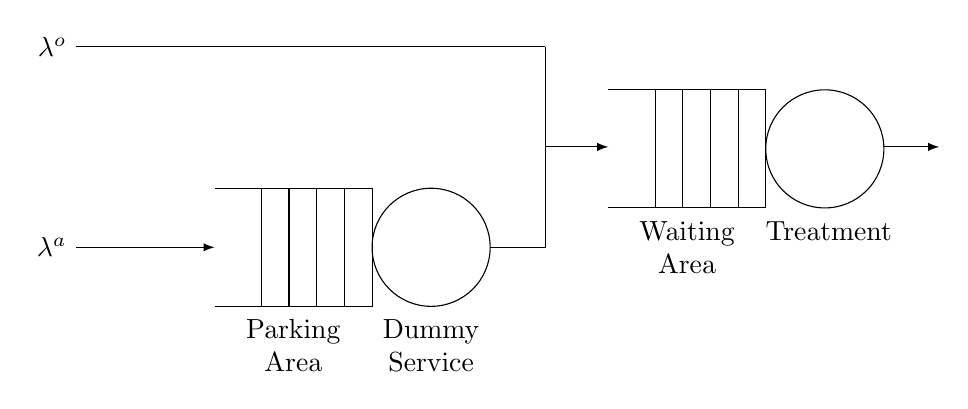
\begin{tikzpicture}[>=latex]
        % the rectangle with vertical rules (Queue 1)
        \draw (0,0) -- ++(2cm,0) -- ++(0,-1.5cm) -- ++(-2cm,0);
        \foreach \i in {1,...,4}
        \draw (2cm-\i*10pt,0) -- +(0,-1.5cm);
        
        % the circle (Queue 1)
        \draw (2.75,-0.75cm) circle [radius=0.75cm];

        % the rectangle with vertical rules (Queue 2)
        \draw (5,1.25) -- ++(2cm,0) -- ++(0,-1.5cm) -- ++(-2cm,0);
        \foreach \i in {1,...,4}
        \draw (7cm-\i*10pt,1.25) -- +(0,-1.5cm);

        % the circle (Queue 2)
        \draw (7.75,0.5) circle [radius=0.75cm];

        % the arrows and labels (Queue 1+2)
        \draw[-] (3.5,-0.75) -- +(20pt,0);
        \draw[<-] (0,-0.75) -- +(-50pt,0) node[left] {\( \lambda^a \)};
        \draw[->] (8.5,0.525) -- +(20pt,0);
        \node[align=center] at (1cm,-2cm) {Parking \\ Area};
        \node[align=center] at (2.75cm,-2cm) {Dummy \\ Service};
        \node[align=center] at (6cm,-0.75cm) {Waiting \\ Area};
        \node[align=center] at (7.8cm,-0.75cm) {Treatment \\ };
        
        \draw (4.2, 1.8) -- +(-169.5pt,0) node[left] {\( \lambda^o \)};
        \draw (4.2, 1.8) -- (4.2, -0.75);
        \draw[->] (4.2, 0.525) -- (5, 0.525);

    \end{tikzpicture}
\end{figure}


\begin{figure}
    \centering
    \begin{tikzpicture}[-, node distance = 1cm, auto, every node/.style={scale=0.5}]

        % Variables
        \tikzmath{
            let \altdist = 1.5cm;
            let \minsz = 1.5cm;
        }

        % First Line
        \node[state, minimum size=1.5cm] (zero) {(0,0)};
        \node[state, minimum size=1.5cm,  right=of zero] (one) {(0,1)};
        \node[draw=none, minimum size=1.5cm, right=of one] (two) {\dots};
        \node[state, minimum size=1.5cm, right=of two] (three) {(0,T)};
        \node[state, node distance = \altdist, minimum size=\minsz, right=of three] (four) {(0,T+1)};
        \node[draw=none, node distance = \altdist, minimum size=\minsz, right=of four] (five) {\dots};
        \node[state, node distance = \altdist, minimum size=\minsz, right=of five] (six) {(0,C)};
        \node[draw=none, minimum size=\minsz, right=of six] (seven) {\dots};

        % Second Line
        \node[state, minimum size=\minsz, below=of three] (three_one) {(1,T)};
        \node[state, minimum size=\minsz, below=of four] (four_one) {(1,T+1)};
        \node[draw=none, minimum size=\minsz, below=of five] (five_one) {\dots};
        \node[state, node distance = \altdist, minimum size=\minsz, right=of five_one] (six_one) {(1,C)};
        \node[draw=none, minimum size=\minsz, right=of six_one] (seven_one) {\dots};

        % Third Line
        \node[state, minimum size=\minsz, below=of three_one] (three_two) {(2,T)};
        \node[state, minimum size=\minsz, below=of four_one] (four_two) {(2,T+1)};
        \node[draw=none, minimum size=\minsz, below=of five_one] (five_two) {\dots};
        \node[state, node distance = \altdist, minimum size=\minsz, right=of five_two] (six_two) {(2,C)};
        \node[draw=none, minimum size=\minsz, right=of six_two] (seven_two) {\dots};

        % Fourth line
        \node[draw=none, minimum size=\minsz, below=of three_two] (three_three) {\vdots};
        \node[draw=none, minimum size=\minsz, below=of four_two] (four_three) {\vdots};
        \node[draw=none, minimum size=\minsz, below=of five_two] (five_three) {};
        \node[draw=none, node distance = \altdist, minimum size=\minsz, right=of five_three] (six_three) {\vdots};

        \draw[every loop]
            % First Horizontal Edges
            (zero) edge[bend left] node {\( \Lambda \)} (one)
            (one) edge[bend left] node [above] {\( \mu \)} (zero)
            (one) edge[bend left] node {\( \Lambda \)} (two)
            (two) edge[bend left] node [above] {\( 2 \mu \)} (one)
            (two) edge[bend left] node {\( \Lambda \)} (three)
            (three) edge[bend left] node [above] {\( T \mu \)} (two)
            (three) edge[bend left] node {\( \lambda^o \)} (four)
            (four) edge[bend left] node [above] {\( (T+1) \mu \)} (three)
            (four) edge[bend left] node {\( \lambda^o \)} (five)
            (five) edge[bend left] node [above] {\( (T+2) \mu \)} (four)
            (five) edge[bend left] node {\( \lambda^o \)} (six)
            (six) edge[bend left] node [above] {\( C\mu \)} (five)
            (six) edge[bend left] node {\( \lambda^o \)} (seven)
            (seven) edge[bend left] node [above] {\( C\mu \)} (six)

            % Second Horizontal Edges
            (three_one) edge[bend left] node {\( \lambda^o \)} (four_one)
            (four_one) edge[bend left] node [above] {\( (T+1) \mu \)} (three_one)
            (four_one) edge[bend left] node {\( \lambda^o \)} (five_one)
            (five_one) edge[bend left] node [above] {\( (T+2) \mu \)} (four_one)
            (five_one) edge[bend left] node {\( \lambda^o \)} (six_one)
            (six_one) edge[bend left] node [above] {\( C\mu \)} (five_one)
            (six_one) edge[bend left] node {\( \lambda^o \)} (seven_one)
            (seven_one) edge[bend left] node [above] {\( C\mu \)} (six_one)

            % Third Horizontal Edges
            (three_two) edge[bend left] node {\( \lambda^o \)} (four_two)
            (four_two) edge[bend left] node [above] {\( (T+1) \mu \)} (three_two)
            (four_two) edge[bend left] node {\( \lambda^o \)} (five_two)
            (five_two) edge[bend left] node [above] {\( (T+2) \mu \)} (four_two)
            (five_two) edge[bend left] node {\( \lambda^o \)} (six_two)
            (six_two) edge[bend left] node [above] {\( C\mu \)} (five_two)
            (six_two) edge[bend left] node {\( \lambda^o \)} (seven_two)
            (seven_two) edge[bend left] node [above] {\( C\mu \)} (six_two)

            % First Vertical Edges
            (three) edge[bend left] node {\( \lambda^A \)} (three_one)
            (three_one) edge[bend left] node {\( T \mu \)} (three)
            (three_one) edge[bend left] node {\( \lambda^A \)} (three_two)
            (three_two) edge[bend left] node {\( T\mu \)} (three_one)
            (three_two) edge[bend left] node {\( \lambda^A \)} (three_three)
            (three_three) edge[bend left] node {\( T\mu \)} (three_two)

            % Second Vertical Edges
            (four) edge node {\( \lambda^A \)} (four_one)
            (four_one) edge node {\( \lambda^A \)} (four_two)
            (four_two) edge node {\( \lambda^A \)} (four_three)

            %Third Vertical Edges
            (six) edge node {\( \lambda^A \)} (six_one)
            (six_one) edge node {\( \lambda^A \)} (six_two)
            (six_two) edge node {\( \lambda^A \)} (six_three)
            ;       
    \end{tikzpicture}
    \caption{Markov chains} 
    \label{Markov_2}
\end{figure}



\begin{figure}
    \centering
    \begin{tikzpicture}[-, node distance = 1cm, auto, every node/.style={scale=0.4}]

        % Variables
        \tikzmath{
            let \altdist = 1cm;
            let \minsz = 1.5cm;
        }

        % First Line
        \node[state, minimum size=1.5cm] (zero) {(0,0)};
        \node[state, minimum size=1.5cm,  right=of zero] (one) {(0,1)};
        \node[draw=none, minimum size=1.5cm, right=of one] (two) {\dots};
        \node[state, minimum size=1.5cm, right=of two] (three) {(0,T)};
        \node[state, node distance = \altdist, minimum size=\minsz, right=of three] (four) {(0,T+1)};
        \node[draw=none, minimum size=\minsz, right=of four] (five) {\dots};
        \node[draw=none, minimum size=\minsz, right=of five] (six) {\vdots};
        \node[draw=none, minimum size=\minsz, right=of six] (seven) {\dots};
        \node[state, minimum size=\minsz, right=of seven] (eight) {(0,C)};
        \node[draw=none, minimum size=\minsz, right=of eight] (nine) {\dots};


        % Second Line
        \node[state, minimum size=\minsz, below=of three] (three_one) {(1,T)};
        \node[state, minimum size=\minsz, below=of four] (four_one) {(1,T+1)};
        \node[draw=none, minimum size=\minsz, below=of five] (five_one) {\dots};
        \node[state, node distance = \altdist, minimum size=\minsz, right=of five_one] (six_one) {\( (u_i, v_i) \)};
        \node[draw=none, minimum size=\minsz, right=of six_one] (seven_one) {\dots};
        \node[state, node distance = \altdist, minimum size=\minsz, right=of seven_one] (eight_one) {(1,C)};
        \node[draw=none, minimum size=\minsz, right=of eight_one] (nine_one) {\dots};
        

        % Third Line
        \node[state, minimum size=\minsz, below=of three_one] (three_two) {(2,T)};
        \node[state, minimum size=\minsz, below=of four_one] (four_two) {(2,T+1)};
        \node[draw=none, minimum size=\minsz, below=of five_one] (five_two) {\dots};
        \node[draw=none, node distance = \altdist, minimum size=\minsz, right=of five_two] (six_two) {\vdots};
        \node[draw=none, minimum size=\minsz, right=of six_two] (seven_two) {\dots};
        \node[state, node distance = \altdist, minimum size=\minsz, right=of seven_two] (eight_two) {(2,C)};
        \node[draw=none, minimum size=\minsz, right=of eight_two] (nine_two) {\dots};

        % Fourth line
        \node[draw=none, minimum size=\minsz, below=of three_two] (three_three) {\vdots};
        \node[draw=none, minimum size=\minsz, below=of four_two] (four_three) {\vdots};
        \node[draw=none, minimum size=\minsz, below=of five_two] (five_three) {};
        \node[draw=none, node distance = \altdist, minimum size=\minsz, right=of five_three] (six_three) {};
        \node[draw=none, node distance = \altdist, minimum size=\minsz, below=of eight_two] (eight_three) {\vdots};


        \draw[every loop]
            % First Horizontal Edges
            (zero) edge[bend left] node {\( \Lambda \)} (one)
            (one) edge[bend left] node {\( \mu \)} (zero)
            (one) edge[bend left] node {\( \Lambda \)} (two)
            (two) edge[bend left] node {\( 2 \mu \)} (one)
            (two) edge[bend left] node {\( \Lambda \)} (three)
            (three) edge[bend left] node {\( T \mu \)} (two)
            (three) edge[bend left] node {\( \lambda^o \)} (four)
            (four) edge[bend left] node {\( (T+1) \mu \)} (three)
            (four) edge[bend left] node {\( \lambda^o \)} (five)
            (five) edge[bend left] node {\( (T+2) \mu \)} (four)
            % (five) edge[bend left] node {\( \lambda^o \)} (six)
            % (six) edge[bend left] node [above] {\( C\mu \)} (five)
            % (six) edge[bend left] node {\( \lambda^o \)} (seven)
            % (seven) edge[bend left] node [above] {\( C\mu \)} (six)
            (seven) edge[bend left] node {\( \lambda^o \)} (eight)
            (eight) edge[bend left] node {\( C\mu \)} (seven)
            (eight) edge[bend left] node {\( \lambda^o \)} (nine)
            (nine) edge[bend left] node {\( C\mu \)} (eight)

            % Second Horizontal Edges
            (three_one) edge[bend left] node {\(\lambda^o\)} (four_one)
            (four_one) edge[bend left] node {\( (T+1) \mu \)} (three_one)
            (four_one) edge[bend left] node {\( \lambda^o \)} (five_one)
            (five_one) edge[bend left] node {\( (T+2) \mu \)} (four_one)
            (five_one) edge[bend left] node {\( \lambda^o \)} (six_one)
            (six_one) edge[bend left] node {\( v_i\mu \)} (five_one)
            (six_one) edge[bend left] node {\( \lambda^o \)} (seven_one)
            (seven_one) edge[bend left] node {\( (v_i+1)\mu \)} (six_one)
            (seven_one) edge[bend left] node {\( \lambda^o \)} (eight_one)
            (eight_one) edge[bend left] node {\( C\mu \)} (seven_one)
            (eight_one) edge[bend left] node {\( \lambda^o \)} (nine_one)
            (nine_one) edge[bend left] node {\( C\mu \)} (eight_one)

            % Third Horizontal Edges
            (three_two) edge[bend left] node {\( \lambda^o \)} (four_two)
            (four_two) edge[bend left] node {\( (T+1) \mu \)} (three_two)
            (four_two) edge[bend left] node {\( \lambda^o \)} (five_two)
            (five_two) edge[bend left] node {\( (T+2) \mu \)} (four_two)
            % (five_two) edge[bend left] node {\( \lambda^o \)} (six_two)
            % (six_two) edge[bend left] node [above] {\( C\mu \)} (five_two)
            % (six_two) edge[bend left] node {\( \lambda^o \)} (seven_two)
            % (seven_two) edge[bend left] node [above] {\( C\mu \)} (six_two)
            (seven_two) edge[bend left] node {\( \lambda^o \)} (eight_two)
            (eight_two) edge[bend left] node {\( C\mu \)} (seven_two)
            (eight_two) edge[bend left] node {\( \lambda^o \)} (nine_two)
            (nine_two) edge[bend left] node {\( C\mu \)} (eight_two)

            % First Vertical Edges
            (three) edge[bend left] node {\( \lambda^A \)} (three_one)
            (three_one) edge[bend left] node {\( T \mu \)} (three)
            (three_one) edge[bend left] node {\( \lambda^A \)} (three_two)
            (three_two) edge[bend left] node {\( T\mu \)} (three_one)
            (three_two) edge[bend left] node {\( \lambda^A \)} (three_three)
            (three_three) edge[bend left] node {\( T\mu \)} (three_two)

            % Second Vertical Edges
            (four) edge node {\( \lambda^A \)} (four_one)
            (four_one) edge node {\( \lambda^A \)} (four_two)
            (four_two) edge node {\( \lambda^A \)} (four_three)

            % Third Vertical Edges
            (six) edge node {\( \lambda^A \)} (six_one)
            (six_one) edge node {\( \lambda^A \)} (six_two)
            % (six_two) edge node {\( \lambda^A \)} (six_three)

            % Fourth Vertical Edges
            (eight) edge node {\( \lambda^A \)} (eight_one)
            (eight_one) edge node {\( \lambda^A \)} (eight_two)
            (eight_two) edge node {\( \lambda^A \)} (eight_three)
            ;       
    \end{tikzpicture}
    \caption{Markov chains} 
    \label{Markov_3}
\end{figure}


\begin{figure}
    \centering
    \begin{tikzpicture}[-, node distance = 0.9cm, auto, every node/.style={scale=0.5}]

        % Variables
        \tikzmath{
            let \initdist = 0.5cm;
            let \altdist = 1.2cm;
            let \minsz = 1.6cm;
            let \leftOne = -0.8;
            let \rightOne = 2.2;
            let \upOne = 0.8;
            let \downOne = -2.2;
            let \leftTwo = 2.25;
            let \rightTwo = 14.2;
            let \upTwo = -2.35;
            let \downTwo = -8.8;
        }

        % % Rectangle for S1
        % \draw[ultra thin, dashed] (\leftOne, \downOne) -- (\leftOne, \upOne);
        % \draw[ultra thin, dashed] (\leftOne, \upOne) -- (\rightOne, \upOne);
        % \draw[ultra thin, dashed] (\rightOne, \upOne) -- node {\Huge{\( \quad S_1 \)}}(\rightOne, \downOne);
        % \draw[ultra thin, dashed] (\rightOne, \downOne) -- (\leftOne, \downOne);

        % % Rectangle for S2
        % \draw[ultra thin, dashed] (\leftTwo, \downTwo) -- node {\Huge{\( S_2 \quad \)}}(\leftTwo, \upTwo);
        % \draw[ultra thin, dashed] (\leftTwo, \upTwo) -- (\rightTwo, \upTwo);
        % \draw[ultra thin, dashed] (\rightTwo, \upTwo) -- (\rightTwo, \downTwo);
        % \draw[ultra thin, dashed] (\rightTwo, \downTwo) -- (\leftTwo, \downTwo);

        % First Line
        \node[state, minimum size=1.5cm] (zero) {(0,0)};
        \node[state, node distance = \initdist, minimum size=\minsz, below right=of zero] (one) {(0,1)};
        \node[draw=none, node distance = \initdist, minimum size=\minsz, below right=of one] (two) {\textbf{\( \ddots \)}};
        \node[state, node distance = \initdist, minimum size=\minsz, below right=of two] (three) {(0,T)};
        \node[state, node distance = \altdist, minimum size=\minsz, right=of three] (four) {(0,T+1)};
        \node[draw=none, node distance = \altdist, minimum size=\minsz, right=of four] (five) {\textbf{\dots}};
        \node[draw=none, minimum size=\minsz, right=of five] (six) {\textbf{\vdots}};
        \node[draw=none, minimum size=\minsz, right=of six] (seven) {\textbf{\dots}};
        \node[state, minimum size=\minsz, right=of seven] (eight) {(0,C)};
        \node[draw=none, minimum size=\minsz, right=of eight] (nine) {\textbf{\dots}};


        % Second Line
        \node[state, minimum size=\minsz, below=of three] (three_one) {(1,T)};
        \node[state, minimum size=\minsz, below=of four] (four_one) {(1,T+1)};
        \node[draw=none, minimum size=\minsz, below=of five] (five_one) {\textbf{\dots}};
        \node[state, minimum size=\minsz, right=of five_one] (six_one) {\( (u_i, v_i) \)};
        \node[draw=none, minimum size=\minsz, right=of six_one] (seven_one) {\textbf{\dots}};
        \node[state, minimum size=\minsz, right=of seven_one] (eight_one) {(1,C)};
        \node[draw=none, minimum size=\minsz, right=of eight_one] (nine_one) {\textbf{\dots}};
        

        % Third Line
        \node[state, minimum size=\minsz, below=of three_one] (three_two) {(2,T)};
        \node[state, minimum size=\minsz, below=of four_one] (four_two) {(2,T+1)};
        \node[draw=none, minimum size=\minsz, below=of five_one] (five_two) {\textbf{\dots}};
        \node[draw=none, minimum size=\minsz, right=of five_two] (six_two) {\textbf{\vdots}};
        \node[draw=none, minimum size=\minsz, right=of six_two] (seven_two) {\textbf{\dots}};
        \node[state, minimum size=\minsz, right=of seven_two] (eight_two) {(2,C)};
        \node[draw=none, minimum size=\minsz, right=of eight_two] (nine_two) {\textbf{\dots}};

        % Fourth line
        \node[draw=none, node distance = \altdist, minimum size=\minsz, below=of three_two] (three_three) {\textbf{\vdots}};
        \node[draw=none, node distance = \altdist, minimum size=\minsz, below=of four_two] (four_three) {\textbf{\vdots}};
        \node[draw=none, node distance = \altdist, minimum size=\minsz, below=of five_two] (five_three) {};
        \node[draw=none, node distance = \altdist, minimum size=\minsz, below=of six_two] (six_three) {};
        \node[draw=none, node distance = \altdist, minimum size=\minsz, below=of eight_two] (eight_three) {\textbf{\vdots}};


        \draw[every loop]
            % First Horizontal Edges
            (zero) edge[bend left] node {\( \Lambda \)} (one)
            (one) edge[bend left] node {\( \mu \)} (zero)
            (one) edge[bend left] node {\( \Lambda \)} (two)
            (two) edge[bend left] node {\( 2 \mu \)} (one)
            (two) edge[bend left] node {\( \Lambda \)} (three)
            (three) edge[bend left] node {\( T \mu \)} (two)
            (three) edge[bend left] node {\( \lambda^o \)} (four)
            (four) edge[bend left] node {\( (T+1) \mu \)} (three)
            (four) edge[bend left] node {\( \lambda^o \)} (five)
            (five) edge[bend left] node {\( (T+2) \mu \)} (four)
            % (five) edge[bend left] node {\( \lambda^o \)} (six)
            % (six) edge[bend left] node [above] {\( C\mu \)} (five)
            % (six) edge[bend left] node {\( \lambda^o \)} (seven)
            % (seven) edge[bend left] node [above] {\( C\mu \)} (six)
            (seven) edge[bend left] node {\( \lambda^o \)} (eight)
            (eight) edge[bend left] node {\( C\mu \)} (seven)
            (eight) edge[bend left] node {\( \lambda^o \)} (nine)
            (nine) edge[bend left] node {\( C\mu \)} (eight)

            % Second Horizontal Edges
            (three_one) edge[bend left] node {\( \lambda^o \)} (four_one)
            (four_one) edge[bend left] node {\( (T+1) \mu \)} (three_one)
            (four_one) edge[bend left] node {\( \lambda^o \)} (five_one)
            (five_one) edge[bend left] node {\( (T+2) \mu \)} (four_one)
            (five_one) edge[bend left] node {\( \lambda^o \)} (six_one)
            (six_one) edge[bend left] node {\( v_i\mu \)} (five_one)
            (six_one) edge[bend left] node {\( \lambda^o \)} (seven_one)
            (seven_one) edge[bend left] node {\( (v_i+1)\mu \)} (six_one)
            (seven_one) edge[bend left] node {\( \lambda^o \)} (eight_one)
            (eight_one) edge[bend left] node {\( C\mu \)} (seven_one)
            (eight_one) edge[bend left] node {\( \lambda^o \)} (nine_one)
            (nine_one) edge[bend left] node {\( C\mu \)} (eight_one)

            % Third Horizontal Edges
            (three_two) edge[bend left] node {\( \lambda^o \)} (four_two)
            (four_two) edge[bend left] node [below] {\( (T+1) \mu \)} (three_two)
            (four_two) edge[bend left] node {\( \lambda^o \)} (five_two)
            (five_two) edge[bend left] node {\( (T+2) \mu \)} (four_two)
            % (five_two) edge[bend left] node {\( \lambda^o \)} (six_two)
            % (six_two) edge[bend left] node [above] {\( C\mu \)} (five_two)
            % (six_two) edge[bend left] node {\( \lambda^o \)} (seven_two)
            % (seven_two) edge[bend left] node [above] {\( C\mu \)} (six_two)
            (seven_two) edge[bend left] node {\( \lambda^o \)} (eight_two)
            (eight_two) edge[bend left] node {\( C\mu \)} (seven_two)
            (eight_two) edge[bend left] node {\( \lambda^o \)} (nine_two)
            (nine_two) edge[bend left] node {\( C\mu \)} (eight_two)

            % First Vertical Edges
            (three) edge[bend left] node {\( \lambda^A \)} (three_one)
            (three_one) edge[bend left] node {\( T \mu \)} (three)
            (three_one) edge[bend left] node {\( \lambda^A \)} (three_two)
            (three_two) edge[bend left] node {\( T\mu \)} (three_one)
            (three_two) edge[bend left] node {\( \lambda^A \)} (three_three)
            (three_three) edge[bend left] node {\( T\mu \)} (three_two)

            % Second Vertical Edges
            (four) edge node {\( \lambda^A \)} (four_one)
            (four_one) edge node {\( \lambda^A \)} (four_two)
            (four_two) edge node {\( \lambda^A \)} (four_three)

            % Third Vertical Edges
            (six) edge node {\( \lambda^A \)} (six_one)
            (six_one) edge node {\( \lambda^A \)} (six_two)
            % (six_two) edge node {\( \lambda^A \)} (six_three)

            % Fourth Vertical Edges
            (eight) edge node {\( \lambda^A \)} (eight_one)
            (eight_one) edge node {\( \lambda^A \)} (eight_two)
            (eight_two) edge node {\( \lambda^A \)} (eight_three)
            ;       
    \end{tikzpicture}
    \caption{Markov chains} 
    \label{Markov_4}
\end{figure}




\begin{figure}
    \centering
    \begin{tikzpicture}[-, node distance = 0.9cm, auto, every node/.style={scale=0.7}]

        % Markov chain variables
        \tikzmath{
            let \initdist = 0.5cm;
            let \altdist = 1.2cm;
            let \minsz = 1.6cm;
        }

        % S_1 and S_2 rectangles
        \tikzmath{
            let \leftOne = -0.8;
            let \rightOne = 2.7;
            let \upOne = 0.8;
            let \downOne = -2.7;
            let \leftTwo = 2.8;
            let \rightTwo = 13;
            let \upTwo = -2.95;
            let \downTwo = -16.4;
        }

        % General case variables
        \tikzmath{
            let \GCsmallx = 8.3;
            let \GCsmally = -9.5;
            let \GCbigx = 4.1;
            let \GCbigy = -11.8;
        }

        % % Rectangle for S1
        % \draw[ultra thin, dashed] (\leftOne, \downOne) -- (\leftOne, \upOne);
        % \draw[ultra thin, dashed] (\leftOne, \upOne) -- (\rightOne, \upOne);
        % \draw[ultra thin, dashed] (\rightOne, \upOne) -- node {\Huge{\( \quad S_1 \)}}(\rightOne, \downOne);
        % \draw[ultra thin, dashed] (\rightOne, \downOne) -- (\leftOne, \downOne);

        % % Rectangle for S2
        % \draw[ultra thin, dashed] (\leftTwo, \downTwo) -- node {\Huge{\( S_2 \quad \)}}(\leftTwo, \upTwo);
        % \draw[ultra thin, dashed] (\leftTwo, \upTwo) -- (\rightTwo, \upTwo);
        % \draw[ultra thin, dashed] (\rightTwo, \upTwo) -- (\rightTwo, \downTwo);
        % \draw[ultra thin, dashed] (\rightTwo, \downTwo) -- (\leftTwo, \downTwo);

        % Small square of general case
        \draw [thick] (\GCsmallx, \GCsmally) -- node {} (\GCsmallx + 0.4, \GCsmally);
        \draw [thick] (\GCsmallx + 0.4, \GCsmally) -- node {} (\GCsmallx + 0.4, \GCsmally - 0.4);
        \draw [thick] (\GCsmallx + 0.4, \GCsmally - 0.4) -- node {} (\GCsmallx, \GCsmally - 0.4);
        \draw [thick] (\GCsmallx, \GCsmally - 0.4) -- node {} (\GCsmallx, \GCsmally);


        % Dashed lines to from small square to big one 
        \draw [ultra thin] (\GCsmallx, \GCsmally) -- node {} (\GCbigx, \GCbigy);
        \draw [ultra thin] (\GCsmallx + 0.4, \GCsmally) -- node {} (\GCbigx + 4, \GCbigy);
        \draw [ultra thin] (\GCsmallx, \GCsmally - 0.4) -- node {} (7, \GCbigy);
        \draw [ultra thin] (\GCsmallx + 0.4, \GCsmally - 0.4) -- node {} (\GCbigx + 4, \GCbigy - 4);
        
        % Big Square of general case
        \draw [ultra thick] (\GCbigx, \GCbigy) -- node {} (\GCbigx + 4, \GCbigy);
        \draw [ultra thick] (\GCbigx + 4, \GCbigy) -- node {} (\GCbigx + 4, \GCbigy - 4);
        \draw [ultra thick] (\GCbigx + 4, \GCbigy - 4) -- node {General Case} (\GCbigx, \GCbigy - 4);
        \draw [ultra thick] (\GCbigx, \GCbigy - 4) -- node {} (\GCbigx, \GCbigy);

        % First Line
        \node[state, minimum size=1.5cm] (zero) {(0,0)};
        \node[state, node distance = \initdist, minimum size=\minsz, below right=of zero] (one) {(0,1)};
        \node[draw=none, node distance = \initdist, minimum size=\minsz, below right=of one] (two) {\textbf{\( \ddots \)}};
        \node[state, node distance = \initdist, minimum size=\minsz, below right=of two] (three) {(0,T)};
        \node[state, node distance = \altdist, minimum size=\minsz, right=of three] (four) {(0,T+1)};
        \node[draw=none, node distance = \altdist, minimum size=\minsz, right=of four] (five) {\textbf{\dots}};
        \node[state, minimum size=\minsz, right=of five] (six) {(0,C)};
        \node[draw=none, minimum size=\minsz, right=of six] (seven) {\textbf{\dots}};

        % Second Line
        \node[state, minimum size=\minsz, below=of three] (three_one) {(1,T)};
        \node[state, minimum size=\minsz, below=of four] (four_one) {(1,T+1)};
        \node[draw=none, minimum size=\minsz, below=of five] (five_one) {\textbf{\dots}};
        \node[state, minimum size=\minsz, right=of five_one] (six_one) {(1,C)};
        \node[draw=none, minimum size=\minsz, right=of six_one] (seven_one) {\textbf{\dots}};
        
        % Third Line
        \node[state, minimum size=\minsz, below=of three_one] (three_two) {(2,T)};
        \node[state, minimum size=\minsz, below=of four_one] (four_two) {(2,T+1)};
        \node[draw=none, minimum size=\minsz, below=of five_one] (five_two) {\textbf{\dots}};
        \node[state, minimum size=\minsz, right=of five_two] (six_two) {(2,C)};
        \node[draw=none, minimum size=\minsz, right=of six_two] (seven_two) {\textbf{\dots}};

        % Fourth line
        \node[draw=none, node distance = \altdist, minimum size=\minsz, below=of three_two] (three_three) {\textbf{\vdots}};
        \node[draw=none, node distance = \altdist, minimum size=\minsz, below=of four_two] (four_three) {\textbf{\vdots}};
        \node[draw=none, node distance = 2cm, minimum size=\minsz, below=of five_two] (five_three) {};
        \node[draw=none, node distance = \altdist, minimum size=\minsz, below=of six_two] (six_three) {\textbf{\vdots}};

        % Fifth line
        % \node[state, node distance = \altdist, minimum size=\minsz, below=of five_three] (general_case_mid) {\( (u_i, v_i) \)};
        \node[draw=none, node distance = 0.3cm, minimum size=\minsz, below=of four_three] (general_case_up) {};
        \node[state, node distance = \altdist, minimum size=\minsz, below=of general_case_up] (general_case_mid) {\( (u_i, v_i) \)};

        \node[draw=none, node distance = \altdist, minimum size=\minsz, below=of general_case_mid] (general_case_down) {};
        \node[draw=none, node distance = \altdist, minimum size=\minsz, left=of general_case_mid] (general_case_left) {};
        \node[draw=none, node distance = \altdist, minimum size=\minsz, right=of general_case_mid] (general_case_right) {};

        \draw[every loop]
            % First Horizontal Edges
            (zero) edge[bend left] node {\( \Lambda \)} (one)
            (one) edge[bend left] node {\( \mu \)} (zero)
            (one) edge[bend left] node {\( \Lambda \)} (two)
            (two) edge[bend left] node {\( 2 \mu \)} (one)
            (two) edge[bend left] node {\( \Lambda \)} (three)
            (three) edge[bend left] node {\( T \mu \)} (two)
            (three) edge[bend left] node {\( \lambda^o \)} (four)
            (four) edge[bend left] node {\( (T+1) \mu \)} (three)
            (four) edge[bend left] node {\( \lambda^o \)} (five)
            (five) edge[bend left] node {\( (T+2) \mu \)} (four)
            (five) edge[bend left] node {\( \lambda^o \)} (six)
            (six) edge[bend left] node {\( C\mu \)} (five)
            (six) edge[bend left] node {\( \lambda^o \)} (seven)
            (seven) edge[bend left] node {\( C\mu \)} (six)

            % Second Horizontal Edges
            (three_one) edge[bend left] node {\( \lambda^o \)} (four_one)
            (four_one) edge[bend left] node {\( (T+1) \mu \)} (three_one)
            (four_one) edge[bend left] node {\( \lambda^o \)} (five_one)
            (five_one) edge[bend left] node {\( (T+2) \mu \)} (four_one)
            (five_one) edge[bend left] node {\( \lambda^o \)} (six_one)
            (six_one) edge[bend left] node {\( C\mu \)} (five_one)
            (six_one) edge[bend left] node {\( \lambda^o \)} (seven_one)
            (seven_one) edge[bend left] node {\( C\mu \)} (six_one)

            % Third Horizontal Edges
            (three_two) edge[bend left] node {\( \lambda^o \)} (four_two)
            (four_two) edge[bend left] node [below] {\( (T+1) \mu \)} (three_two)
            (four_two) edge[bend left] node {\( \lambda^o \)} (five_two)
            (five_two) edge[bend left] node {\( (T+2) \mu \)} (four_two)
            (five_two) edge[bend left] node {\( \lambda^o \)} (six_two)
            (six_two) edge[bend left] node {\( C\mu \)} (five_two)
            (six_two) edge[bend left] node {\( \lambda^o \)} (seven_two)
            (seven_two) edge[bend left] node {\( C\mu \)} (six_two)

            % First Vertical Edges
            (three) edge[bend left] node {\( \lambda^A \)} (three_one)
            (three_one) edge[bend left] node {\( T \mu \)} (three)
            (three_one) edge[bend left] node {\( \lambda^A \)} (three_two)
            (three_two) edge[bend left] node {\( T\mu \)} (three_one)
            (three_two) edge[bend left] node {\( \lambda^A \)} (three_three)
            (three_three) edge[bend left] node {\( T\mu \)} (three_two)

            % Second Vertical Edges
            (four) edge node {\( \lambda^A \)} (four_one)
            (four_one) edge node {\( \lambda^A \)} (four_two)
            (four_two) edge node {\( \lambda^A \)} (four_three)

            % Fourth Vertical Edges
            (six) edge node {\( \lambda^A \)} (six_one)
            (six_one) edge node {\( \lambda^A \)} (six_two)
            (six_two) edge node {\( \lambda^A \)} (six_three)

            % General Case
            (general_case_left) edge[bend left] node {\( \lambda^o \)} (general_case_mid)
            (general_case_mid) edge[bend left] node {\( v_i \mu \)} (general_case_left)
            (general_case_right) edge[bend left] node {\( (v_i +1) \mu \)} (general_case_mid)
            (general_case_mid) edge[bend left] node {\( \lambda_o \)} (general_case_right)
            % (five_three) edge node {\( \lambda_A \)} (general_case_mid)
            (general_case_up) edge node {\( \lambda_A \)} (general_case_mid)
            (general_case_mid) edge node {\( \lambda_A \)} (general_case_down)
            ;
    \end{tikzpicture}
    \caption{Markov chain} 
    \label{Markov_5}
\end{figure}

}
        \caption{\(M=2\)}
    \end{figure}
    \begin{figure}[H]
        \centering
        \scalebox{0.8}{
            \section{Figures that might be useful}
\begin{figure}[h]
    \centering
    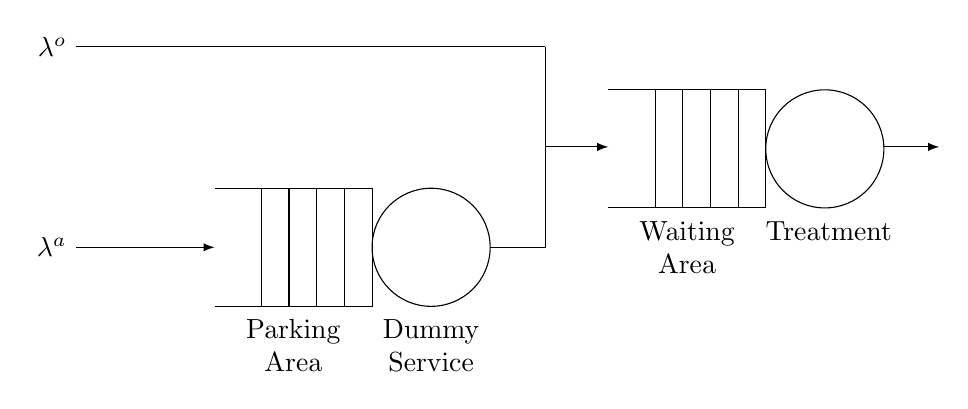
\begin{tikzpicture}[>=latex]
        % the rectangle with vertical rules (Queue 1)
        \draw (0,0) -- ++(2cm,0) -- ++(0,-1.5cm) -- ++(-2cm,0);
        \foreach \i in {1,...,4}
        \draw (2cm-\i*10pt,0) -- +(0,-1.5cm);
        
        % the circle (Queue 1)
        \draw (2.75,-0.75cm) circle [radius=0.75cm];

        % the rectangle with vertical rules (Queue 2)
        \draw (5,1.25) -- ++(2cm,0) -- ++(0,-1.5cm) -- ++(-2cm,0);
        \foreach \i in {1,...,4}
        \draw (7cm-\i*10pt,1.25) -- +(0,-1.5cm);

        % the circle (Queue 2)
        \draw (7.75,0.5) circle [radius=0.75cm];

        % the arrows and labels (Queue 1+2)
        \draw[-] (3.5,-0.75) -- +(20pt,0);
        \draw[<-] (0,-0.75) -- +(-50pt,0) node[left] {\( \lambda^a \)};
        \draw[->] (8.5,0.525) -- +(20pt,0);
        \node[align=center] at (1cm,-2cm) {Parking \\ Area};
        \node[align=center] at (2.75cm,-2cm) {Dummy \\ Service};
        \node[align=center] at (6cm,-0.75cm) {Waiting \\ Area};
        \node[align=center] at (7.8cm,-0.75cm) {Treatment \\ };
        
        \draw (4.2, 1.8) -- +(-169.5pt,0) node[left] {\( \lambda^o \)};
        \draw (4.2, 1.8) -- (4.2, -0.75);
        \draw[->] (4.2, 0.525) -- (5, 0.525);

    \end{tikzpicture}
\end{figure}


\begin{figure}
    \centering
    \begin{tikzpicture}[-, node distance = 1cm, auto, every node/.style={scale=0.5}]

        % Variables
        \tikzmath{
            let \altdist = 1.5cm;
            let \minsz = 1.5cm;
        }

        % First Line
        \node[state, minimum size=1.5cm] (zero) {(0,0)};
        \node[state, minimum size=1.5cm,  right=of zero] (one) {(0,1)};
        \node[draw=none, minimum size=1.5cm, right=of one] (two) {\dots};
        \node[state, minimum size=1.5cm, right=of two] (three) {(0,T)};
        \node[state, node distance = \altdist, minimum size=\minsz, right=of three] (four) {(0,T+1)};
        \node[draw=none, node distance = \altdist, minimum size=\minsz, right=of four] (five) {\dots};
        \node[state, node distance = \altdist, minimum size=\minsz, right=of five] (six) {(0,C)};
        \node[draw=none, minimum size=\minsz, right=of six] (seven) {\dots};

        % Second Line
        \node[state, minimum size=\minsz, below=of three] (three_one) {(1,T)};
        \node[state, minimum size=\minsz, below=of four] (four_one) {(1,T+1)};
        \node[draw=none, minimum size=\minsz, below=of five] (five_one) {\dots};
        \node[state, node distance = \altdist, minimum size=\minsz, right=of five_one] (six_one) {(1,C)};
        \node[draw=none, minimum size=\minsz, right=of six_one] (seven_one) {\dots};

        % Third Line
        \node[state, minimum size=\minsz, below=of three_one] (three_two) {(2,T)};
        \node[state, minimum size=\minsz, below=of four_one] (four_two) {(2,T+1)};
        \node[draw=none, minimum size=\minsz, below=of five_one] (five_two) {\dots};
        \node[state, node distance = \altdist, minimum size=\minsz, right=of five_two] (six_two) {(2,C)};
        \node[draw=none, minimum size=\minsz, right=of six_two] (seven_two) {\dots};

        % Fourth line
        \node[draw=none, minimum size=\minsz, below=of three_two] (three_three) {\vdots};
        \node[draw=none, minimum size=\minsz, below=of four_two] (four_three) {\vdots};
        \node[draw=none, minimum size=\minsz, below=of five_two] (five_three) {};
        \node[draw=none, node distance = \altdist, minimum size=\minsz, right=of five_three] (six_three) {\vdots};

        \draw[every loop]
            % First Horizontal Edges
            (zero) edge[bend left] node {\( \Lambda \)} (one)
            (one) edge[bend left] node [above] {\( \mu \)} (zero)
            (one) edge[bend left] node {\( \Lambda \)} (two)
            (two) edge[bend left] node [above] {\( 2 \mu \)} (one)
            (two) edge[bend left] node {\( \Lambda \)} (three)
            (three) edge[bend left] node [above] {\( T \mu \)} (two)
            (three) edge[bend left] node {\( \lambda^o \)} (four)
            (four) edge[bend left] node [above] {\( (T+1) \mu \)} (three)
            (four) edge[bend left] node {\( \lambda^o \)} (five)
            (five) edge[bend left] node [above] {\( (T+2) \mu \)} (four)
            (five) edge[bend left] node {\( \lambda^o \)} (six)
            (six) edge[bend left] node [above] {\( C\mu \)} (five)
            (six) edge[bend left] node {\( \lambda^o \)} (seven)
            (seven) edge[bend left] node [above] {\( C\mu \)} (six)

            % Second Horizontal Edges
            (three_one) edge[bend left] node {\( \lambda^o \)} (four_one)
            (four_one) edge[bend left] node [above] {\( (T+1) \mu \)} (three_one)
            (four_one) edge[bend left] node {\( \lambda^o \)} (five_one)
            (five_one) edge[bend left] node [above] {\( (T+2) \mu \)} (four_one)
            (five_one) edge[bend left] node {\( \lambda^o \)} (six_one)
            (six_one) edge[bend left] node [above] {\( C\mu \)} (five_one)
            (six_one) edge[bend left] node {\( \lambda^o \)} (seven_one)
            (seven_one) edge[bend left] node [above] {\( C\mu \)} (six_one)

            % Third Horizontal Edges
            (three_two) edge[bend left] node {\( \lambda^o \)} (four_two)
            (four_two) edge[bend left] node [above] {\( (T+1) \mu \)} (three_two)
            (four_two) edge[bend left] node {\( \lambda^o \)} (five_two)
            (five_two) edge[bend left] node [above] {\( (T+2) \mu \)} (four_two)
            (five_two) edge[bend left] node {\( \lambda^o \)} (six_two)
            (six_two) edge[bend left] node [above] {\( C\mu \)} (five_two)
            (six_two) edge[bend left] node {\( \lambda^o \)} (seven_two)
            (seven_two) edge[bend left] node [above] {\( C\mu \)} (six_two)

            % First Vertical Edges
            (three) edge[bend left] node {\( \lambda^A \)} (three_one)
            (three_one) edge[bend left] node {\( T \mu \)} (three)
            (three_one) edge[bend left] node {\( \lambda^A \)} (three_two)
            (three_two) edge[bend left] node {\( T\mu \)} (three_one)
            (three_two) edge[bend left] node {\( \lambda^A \)} (three_three)
            (three_three) edge[bend left] node {\( T\mu \)} (three_two)

            % Second Vertical Edges
            (four) edge node {\( \lambda^A \)} (four_one)
            (four_one) edge node {\( \lambda^A \)} (four_two)
            (four_two) edge node {\( \lambda^A \)} (four_three)

            %Third Vertical Edges
            (six) edge node {\( \lambda^A \)} (six_one)
            (six_one) edge node {\( \lambda^A \)} (six_two)
            (six_two) edge node {\( \lambda^A \)} (six_three)
            ;       
    \end{tikzpicture}
    \caption{Markov chains} 
    \label{Markov_2}
\end{figure}



\begin{figure}
    \centering
    \begin{tikzpicture}[-, node distance = 1cm, auto, every node/.style={scale=0.4}]

        % Variables
        \tikzmath{
            let \altdist = 1cm;
            let \minsz = 1.5cm;
        }

        % First Line
        \node[state, minimum size=1.5cm] (zero) {(0,0)};
        \node[state, minimum size=1.5cm,  right=of zero] (one) {(0,1)};
        \node[draw=none, minimum size=1.5cm, right=of one] (two) {\dots};
        \node[state, minimum size=1.5cm, right=of two] (three) {(0,T)};
        \node[state, node distance = \altdist, minimum size=\minsz, right=of three] (four) {(0,T+1)};
        \node[draw=none, minimum size=\minsz, right=of four] (five) {\dots};
        \node[draw=none, minimum size=\minsz, right=of five] (six) {\vdots};
        \node[draw=none, minimum size=\minsz, right=of six] (seven) {\dots};
        \node[state, minimum size=\minsz, right=of seven] (eight) {(0,C)};
        \node[draw=none, minimum size=\minsz, right=of eight] (nine) {\dots};


        % Second Line
        \node[state, minimum size=\minsz, below=of three] (three_one) {(1,T)};
        \node[state, minimum size=\minsz, below=of four] (four_one) {(1,T+1)};
        \node[draw=none, minimum size=\minsz, below=of five] (five_one) {\dots};
        \node[state, node distance = \altdist, minimum size=\minsz, right=of five_one] (six_one) {\( (u_i, v_i) \)};
        \node[draw=none, minimum size=\minsz, right=of six_one] (seven_one) {\dots};
        \node[state, node distance = \altdist, minimum size=\minsz, right=of seven_one] (eight_one) {(1,C)};
        \node[draw=none, minimum size=\minsz, right=of eight_one] (nine_one) {\dots};
        

        % Third Line
        \node[state, minimum size=\minsz, below=of three_one] (three_two) {(2,T)};
        \node[state, minimum size=\minsz, below=of four_one] (four_two) {(2,T+1)};
        \node[draw=none, minimum size=\minsz, below=of five_one] (five_two) {\dots};
        \node[draw=none, node distance = \altdist, minimum size=\minsz, right=of five_two] (six_two) {\vdots};
        \node[draw=none, minimum size=\minsz, right=of six_two] (seven_two) {\dots};
        \node[state, node distance = \altdist, minimum size=\minsz, right=of seven_two] (eight_two) {(2,C)};
        \node[draw=none, minimum size=\minsz, right=of eight_two] (nine_two) {\dots};

        % Fourth line
        \node[draw=none, minimum size=\minsz, below=of three_two] (three_three) {\vdots};
        \node[draw=none, minimum size=\minsz, below=of four_two] (four_three) {\vdots};
        \node[draw=none, minimum size=\minsz, below=of five_two] (five_three) {};
        \node[draw=none, node distance = \altdist, minimum size=\minsz, right=of five_three] (six_three) {};
        \node[draw=none, node distance = \altdist, minimum size=\minsz, below=of eight_two] (eight_three) {\vdots};


        \draw[every loop]
            % First Horizontal Edges
            (zero) edge[bend left] node {\( \Lambda \)} (one)
            (one) edge[bend left] node {\( \mu \)} (zero)
            (one) edge[bend left] node {\( \Lambda \)} (two)
            (two) edge[bend left] node {\( 2 \mu \)} (one)
            (two) edge[bend left] node {\( \Lambda \)} (three)
            (three) edge[bend left] node {\( T \mu \)} (two)
            (three) edge[bend left] node {\( \lambda^o \)} (four)
            (four) edge[bend left] node {\( (T+1) \mu \)} (three)
            (four) edge[bend left] node {\( \lambda^o \)} (five)
            (five) edge[bend left] node {\( (T+2) \mu \)} (four)
            % (five) edge[bend left] node {\( \lambda^o \)} (six)
            % (six) edge[bend left] node [above] {\( C\mu \)} (five)
            % (six) edge[bend left] node {\( \lambda^o \)} (seven)
            % (seven) edge[bend left] node [above] {\( C\mu \)} (six)
            (seven) edge[bend left] node {\( \lambda^o \)} (eight)
            (eight) edge[bend left] node {\( C\mu \)} (seven)
            (eight) edge[bend left] node {\( \lambda^o \)} (nine)
            (nine) edge[bend left] node {\( C\mu \)} (eight)

            % Second Horizontal Edges
            (three_one) edge[bend left] node {\(\lambda^o\)} (four_one)
            (four_one) edge[bend left] node {\( (T+1) \mu \)} (three_one)
            (four_one) edge[bend left] node {\( \lambda^o \)} (five_one)
            (five_one) edge[bend left] node {\( (T+2) \mu \)} (four_one)
            (five_one) edge[bend left] node {\( \lambda^o \)} (six_one)
            (six_one) edge[bend left] node {\( v_i\mu \)} (five_one)
            (six_one) edge[bend left] node {\( \lambda^o \)} (seven_one)
            (seven_one) edge[bend left] node {\( (v_i+1)\mu \)} (six_one)
            (seven_one) edge[bend left] node {\( \lambda^o \)} (eight_one)
            (eight_one) edge[bend left] node {\( C\mu \)} (seven_one)
            (eight_one) edge[bend left] node {\( \lambda^o \)} (nine_one)
            (nine_one) edge[bend left] node {\( C\mu \)} (eight_one)

            % Third Horizontal Edges
            (three_two) edge[bend left] node {\( \lambda^o \)} (four_two)
            (four_two) edge[bend left] node {\( (T+1) \mu \)} (three_two)
            (four_two) edge[bend left] node {\( \lambda^o \)} (five_two)
            (five_two) edge[bend left] node {\( (T+2) \mu \)} (four_two)
            % (five_two) edge[bend left] node {\( \lambda^o \)} (six_two)
            % (six_two) edge[bend left] node [above] {\( C\mu \)} (five_two)
            % (six_two) edge[bend left] node {\( \lambda^o \)} (seven_two)
            % (seven_two) edge[bend left] node [above] {\( C\mu \)} (six_two)
            (seven_two) edge[bend left] node {\( \lambda^o \)} (eight_two)
            (eight_two) edge[bend left] node {\( C\mu \)} (seven_two)
            (eight_two) edge[bend left] node {\( \lambda^o \)} (nine_two)
            (nine_two) edge[bend left] node {\( C\mu \)} (eight_two)

            % First Vertical Edges
            (three) edge[bend left] node {\( \lambda^A \)} (three_one)
            (three_one) edge[bend left] node {\( T \mu \)} (three)
            (three_one) edge[bend left] node {\( \lambda^A \)} (three_two)
            (three_two) edge[bend left] node {\( T\mu \)} (three_one)
            (three_two) edge[bend left] node {\( \lambda^A \)} (three_three)
            (three_three) edge[bend left] node {\( T\mu \)} (three_two)

            % Second Vertical Edges
            (four) edge node {\( \lambda^A \)} (four_one)
            (four_one) edge node {\( \lambda^A \)} (four_two)
            (four_two) edge node {\( \lambda^A \)} (four_three)

            % Third Vertical Edges
            (six) edge node {\( \lambda^A \)} (six_one)
            (six_one) edge node {\( \lambda^A \)} (six_two)
            % (six_two) edge node {\( \lambda^A \)} (six_three)

            % Fourth Vertical Edges
            (eight) edge node {\( \lambda^A \)} (eight_one)
            (eight_one) edge node {\( \lambda^A \)} (eight_two)
            (eight_two) edge node {\( \lambda^A \)} (eight_three)
            ;       
    \end{tikzpicture}
    \caption{Markov chains} 
    \label{Markov_3}
\end{figure}


\begin{figure}
    \centering
    \begin{tikzpicture}[-, node distance = 0.9cm, auto, every node/.style={scale=0.5}]

        % Variables
        \tikzmath{
            let \initdist = 0.5cm;
            let \altdist = 1.2cm;
            let \minsz = 1.6cm;
            let \leftOne = -0.8;
            let \rightOne = 2.2;
            let \upOne = 0.8;
            let \downOne = -2.2;
            let \leftTwo = 2.25;
            let \rightTwo = 14.2;
            let \upTwo = -2.35;
            let \downTwo = -8.8;
        }

        % % Rectangle for S1
        % \draw[ultra thin, dashed] (\leftOne, \downOne) -- (\leftOne, \upOne);
        % \draw[ultra thin, dashed] (\leftOne, \upOne) -- (\rightOne, \upOne);
        % \draw[ultra thin, dashed] (\rightOne, \upOne) -- node {\Huge{\( \quad S_1 \)}}(\rightOne, \downOne);
        % \draw[ultra thin, dashed] (\rightOne, \downOne) -- (\leftOne, \downOne);

        % % Rectangle for S2
        % \draw[ultra thin, dashed] (\leftTwo, \downTwo) -- node {\Huge{\( S_2 \quad \)}}(\leftTwo, \upTwo);
        % \draw[ultra thin, dashed] (\leftTwo, \upTwo) -- (\rightTwo, \upTwo);
        % \draw[ultra thin, dashed] (\rightTwo, \upTwo) -- (\rightTwo, \downTwo);
        % \draw[ultra thin, dashed] (\rightTwo, \downTwo) -- (\leftTwo, \downTwo);

        % First Line
        \node[state, minimum size=1.5cm] (zero) {(0,0)};
        \node[state, node distance = \initdist, minimum size=\minsz, below right=of zero] (one) {(0,1)};
        \node[draw=none, node distance = \initdist, minimum size=\minsz, below right=of one] (two) {\textbf{\( \ddots \)}};
        \node[state, node distance = \initdist, minimum size=\minsz, below right=of two] (three) {(0,T)};
        \node[state, node distance = \altdist, minimum size=\minsz, right=of three] (four) {(0,T+1)};
        \node[draw=none, node distance = \altdist, minimum size=\minsz, right=of four] (five) {\textbf{\dots}};
        \node[draw=none, minimum size=\minsz, right=of five] (six) {\textbf{\vdots}};
        \node[draw=none, minimum size=\minsz, right=of six] (seven) {\textbf{\dots}};
        \node[state, minimum size=\minsz, right=of seven] (eight) {(0,C)};
        \node[draw=none, minimum size=\minsz, right=of eight] (nine) {\textbf{\dots}};


        % Second Line
        \node[state, minimum size=\minsz, below=of three] (three_one) {(1,T)};
        \node[state, minimum size=\minsz, below=of four] (four_one) {(1,T+1)};
        \node[draw=none, minimum size=\minsz, below=of five] (five_one) {\textbf{\dots}};
        \node[state, minimum size=\minsz, right=of five_one] (six_one) {\( (u_i, v_i) \)};
        \node[draw=none, minimum size=\minsz, right=of six_one] (seven_one) {\textbf{\dots}};
        \node[state, minimum size=\minsz, right=of seven_one] (eight_one) {(1,C)};
        \node[draw=none, minimum size=\minsz, right=of eight_one] (nine_one) {\textbf{\dots}};
        

        % Third Line
        \node[state, minimum size=\minsz, below=of three_one] (three_two) {(2,T)};
        \node[state, minimum size=\minsz, below=of four_one] (four_two) {(2,T+1)};
        \node[draw=none, minimum size=\minsz, below=of five_one] (five_two) {\textbf{\dots}};
        \node[draw=none, minimum size=\minsz, right=of five_two] (six_two) {\textbf{\vdots}};
        \node[draw=none, minimum size=\minsz, right=of six_two] (seven_two) {\textbf{\dots}};
        \node[state, minimum size=\minsz, right=of seven_two] (eight_two) {(2,C)};
        \node[draw=none, minimum size=\minsz, right=of eight_two] (nine_two) {\textbf{\dots}};

        % Fourth line
        \node[draw=none, node distance = \altdist, minimum size=\minsz, below=of three_two] (three_three) {\textbf{\vdots}};
        \node[draw=none, node distance = \altdist, minimum size=\minsz, below=of four_two] (four_three) {\textbf{\vdots}};
        \node[draw=none, node distance = \altdist, minimum size=\minsz, below=of five_two] (five_three) {};
        \node[draw=none, node distance = \altdist, minimum size=\minsz, below=of six_two] (six_three) {};
        \node[draw=none, node distance = \altdist, minimum size=\minsz, below=of eight_two] (eight_three) {\textbf{\vdots}};


        \draw[every loop]
            % First Horizontal Edges
            (zero) edge[bend left] node {\( \Lambda \)} (one)
            (one) edge[bend left] node {\( \mu \)} (zero)
            (one) edge[bend left] node {\( \Lambda \)} (two)
            (two) edge[bend left] node {\( 2 \mu \)} (one)
            (two) edge[bend left] node {\( \Lambda \)} (three)
            (three) edge[bend left] node {\( T \mu \)} (two)
            (three) edge[bend left] node {\( \lambda^o \)} (four)
            (four) edge[bend left] node {\( (T+1) \mu \)} (three)
            (four) edge[bend left] node {\( \lambda^o \)} (five)
            (five) edge[bend left] node {\( (T+2) \mu \)} (four)
            % (five) edge[bend left] node {\( \lambda^o \)} (six)
            % (six) edge[bend left] node [above] {\( C\mu \)} (five)
            % (six) edge[bend left] node {\( \lambda^o \)} (seven)
            % (seven) edge[bend left] node [above] {\( C\mu \)} (six)
            (seven) edge[bend left] node {\( \lambda^o \)} (eight)
            (eight) edge[bend left] node {\( C\mu \)} (seven)
            (eight) edge[bend left] node {\( \lambda^o \)} (nine)
            (nine) edge[bend left] node {\( C\mu \)} (eight)

            % Second Horizontal Edges
            (three_one) edge[bend left] node {\( \lambda^o \)} (four_one)
            (four_one) edge[bend left] node {\( (T+1) \mu \)} (three_one)
            (four_one) edge[bend left] node {\( \lambda^o \)} (five_one)
            (five_one) edge[bend left] node {\( (T+2) \mu \)} (four_one)
            (five_one) edge[bend left] node {\( \lambda^o \)} (six_one)
            (six_one) edge[bend left] node {\( v_i\mu \)} (five_one)
            (six_one) edge[bend left] node {\( \lambda^o \)} (seven_one)
            (seven_one) edge[bend left] node {\( (v_i+1)\mu \)} (six_one)
            (seven_one) edge[bend left] node {\( \lambda^o \)} (eight_one)
            (eight_one) edge[bend left] node {\( C\mu \)} (seven_one)
            (eight_one) edge[bend left] node {\( \lambda^o \)} (nine_one)
            (nine_one) edge[bend left] node {\( C\mu \)} (eight_one)

            % Third Horizontal Edges
            (three_two) edge[bend left] node {\( \lambda^o \)} (four_two)
            (four_two) edge[bend left] node [below] {\( (T+1) \mu \)} (three_two)
            (four_two) edge[bend left] node {\( \lambda^o \)} (five_two)
            (five_two) edge[bend left] node {\( (T+2) \mu \)} (four_two)
            % (five_two) edge[bend left] node {\( \lambda^o \)} (six_two)
            % (six_two) edge[bend left] node [above] {\( C\mu \)} (five_two)
            % (six_two) edge[bend left] node {\( \lambda^o \)} (seven_two)
            % (seven_two) edge[bend left] node [above] {\( C\mu \)} (six_two)
            (seven_two) edge[bend left] node {\( \lambda^o \)} (eight_two)
            (eight_two) edge[bend left] node {\( C\mu \)} (seven_two)
            (eight_two) edge[bend left] node {\( \lambda^o \)} (nine_two)
            (nine_two) edge[bend left] node {\( C\mu \)} (eight_two)

            % First Vertical Edges
            (three) edge[bend left] node {\( \lambda^A \)} (three_one)
            (three_one) edge[bend left] node {\( T \mu \)} (three)
            (three_one) edge[bend left] node {\( \lambda^A \)} (three_two)
            (three_two) edge[bend left] node {\( T\mu \)} (three_one)
            (three_two) edge[bend left] node {\( \lambda^A \)} (three_three)
            (three_three) edge[bend left] node {\( T\mu \)} (three_two)

            % Second Vertical Edges
            (four) edge node {\( \lambda^A \)} (four_one)
            (four_one) edge node {\( \lambda^A \)} (four_two)
            (four_two) edge node {\( \lambda^A \)} (four_three)

            % Third Vertical Edges
            (six) edge node {\( \lambda^A \)} (six_one)
            (six_one) edge node {\( \lambda^A \)} (six_two)
            % (six_two) edge node {\( \lambda^A \)} (six_three)

            % Fourth Vertical Edges
            (eight) edge node {\( \lambda^A \)} (eight_one)
            (eight_one) edge node {\( \lambda^A \)} (eight_two)
            (eight_two) edge node {\( \lambda^A \)} (eight_three)
            ;       
    \end{tikzpicture}
    \caption{Markov chains} 
    \label{Markov_4}
\end{figure}




\begin{figure}
    \centering
    \begin{tikzpicture}[-, node distance = 0.9cm, auto, every node/.style={scale=0.7}]

        % Markov chain variables
        \tikzmath{
            let \initdist = 0.5cm;
            let \altdist = 1.2cm;
            let \minsz = 1.6cm;
        }

        % S_1 and S_2 rectangles
        \tikzmath{
            let \leftOne = -0.8;
            let \rightOne = 2.7;
            let \upOne = 0.8;
            let \downOne = -2.7;
            let \leftTwo = 2.8;
            let \rightTwo = 13;
            let \upTwo = -2.95;
            let \downTwo = -16.4;
        }

        % General case variables
        \tikzmath{
            let \GCsmallx = 8.3;
            let \GCsmally = -9.5;
            let \GCbigx = 4.1;
            let \GCbigy = -11.8;
        }

        % % Rectangle for S1
        % \draw[ultra thin, dashed] (\leftOne, \downOne) -- (\leftOne, \upOne);
        % \draw[ultra thin, dashed] (\leftOne, \upOne) -- (\rightOne, \upOne);
        % \draw[ultra thin, dashed] (\rightOne, \upOne) -- node {\Huge{\( \quad S_1 \)}}(\rightOne, \downOne);
        % \draw[ultra thin, dashed] (\rightOne, \downOne) -- (\leftOne, \downOne);

        % % Rectangle for S2
        % \draw[ultra thin, dashed] (\leftTwo, \downTwo) -- node {\Huge{\( S_2 \quad \)}}(\leftTwo, \upTwo);
        % \draw[ultra thin, dashed] (\leftTwo, \upTwo) -- (\rightTwo, \upTwo);
        % \draw[ultra thin, dashed] (\rightTwo, \upTwo) -- (\rightTwo, \downTwo);
        % \draw[ultra thin, dashed] (\rightTwo, \downTwo) -- (\leftTwo, \downTwo);

        % Small square of general case
        \draw [thick] (\GCsmallx, \GCsmally) -- node {} (\GCsmallx + 0.4, \GCsmally);
        \draw [thick] (\GCsmallx + 0.4, \GCsmally) -- node {} (\GCsmallx + 0.4, \GCsmally - 0.4);
        \draw [thick] (\GCsmallx + 0.4, \GCsmally - 0.4) -- node {} (\GCsmallx, \GCsmally - 0.4);
        \draw [thick] (\GCsmallx, \GCsmally - 0.4) -- node {} (\GCsmallx, \GCsmally);


        % Dashed lines to from small square to big one 
        \draw [ultra thin] (\GCsmallx, \GCsmally) -- node {} (\GCbigx, \GCbigy);
        \draw [ultra thin] (\GCsmallx + 0.4, \GCsmally) -- node {} (\GCbigx + 4, \GCbigy);
        \draw [ultra thin] (\GCsmallx, \GCsmally - 0.4) -- node {} (7, \GCbigy);
        \draw [ultra thin] (\GCsmallx + 0.4, \GCsmally - 0.4) -- node {} (\GCbigx + 4, \GCbigy - 4);
        
        % Big Square of general case
        \draw [ultra thick] (\GCbigx, \GCbigy) -- node {} (\GCbigx + 4, \GCbigy);
        \draw [ultra thick] (\GCbigx + 4, \GCbigy) -- node {} (\GCbigx + 4, \GCbigy - 4);
        \draw [ultra thick] (\GCbigx + 4, \GCbigy - 4) -- node {General Case} (\GCbigx, \GCbigy - 4);
        \draw [ultra thick] (\GCbigx, \GCbigy - 4) -- node {} (\GCbigx, \GCbigy);

        % First Line
        \node[state, minimum size=1.5cm] (zero) {(0,0)};
        \node[state, node distance = \initdist, minimum size=\minsz, below right=of zero] (one) {(0,1)};
        \node[draw=none, node distance = \initdist, minimum size=\minsz, below right=of one] (two) {\textbf{\( \ddots \)}};
        \node[state, node distance = \initdist, minimum size=\minsz, below right=of two] (three) {(0,T)};
        \node[state, node distance = \altdist, minimum size=\minsz, right=of three] (four) {(0,T+1)};
        \node[draw=none, node distance = \altdist, minimum size=\minsz, right=of four] (five) {\textbf{\dots}};
        \node[state, minimum size=\minsz, right=of five] (six) {(0,C)};
        \node[draw=none, minimum size=\minsz, right=of six] (seven) {\textbf{\dots}};

        % Second Line
        \node[state, minimum size=\minsz, below=of three] (three_one) {(1,T)};
        \node[state, minimum size=\minsz, below=of four] (four_one) {(1,T+1)};
        \node[draw=none, minimum size=\minsz, below=of five] (five_one) {\textbf{\dots}};
        \node[state, minimum size=\minsz, right=of five_one] (six_one) {(1,C)};
        \node[draw=none, minimum size=\minsz, right=of six_one] (seven_one) {\textbf{\dots}};
        
        % Third Line
        \node[state, minimum size=\minsz, below=of three_one] (three_two) {(2,T)};
        \node[state, minimum size=\minsz, below=of four_one] (four_two) {(2,T+1)};
        \node[draw=none, minimum size=\minsz, below=of five_one] (five_two) {\textbf{\dots}};
        \node[state, minimum size=\minsz, right=of five_two] (six_two) {(2,C)};
        \node[draw=none, minimum size=\minsz, right=of six_two] (seven_two) {\textbf{\dots}};

        % Fourth line
        \node[draw=none, node distance = \altdist, minimum size=\minsz, below=of three_two] (three_three) {\textbf{\vdots}};
        \node[draw=none, node distance = \altdist, minimum size=\minsz, below=of four_two] (four_three) {\textbf{\vdots}};
        \node[draw=none, node distance = 2cm, minimum size=\minsz, below=of five_two] (five_three) {};
        \node[draw=none, node distance = \altdist, minimum size=\minsz, below=of six_two] (six_three) {\textbf{\vdots}};

        % Fifth line
        % \node[state, node distance = \altdist, minimum size=\minsz, below=of five_three] (general_case_mid) {\( (u_i, v_i) \)};
        \node[draw=none, node distance = 0.3cm, minimum size=\minsz, below=of four_three] (general_case_up) {};
        \node[state, node distance = \altdist, minimum size=\minsz, below=of general_case_up] (general_case_mid) {\( (u_i, v_i) \)};

        \node[draw=none, node distance = \altdist, minimum size=\minsz, below=of general_case_mid] (general_case_down) {};
        \node[draw=none, node distance = \altdist, minimum size=\minsz, left=of general_case_mid] (general_case_left) {};
        \node[draw=none, node distance = \altdist, minimum size=\minsz, right=of general_case_mid] (general_case_right) {};

        \draw[every loop]
            % First Horizontal Edges
            (zero) edge[bend left] node {\( \Lambda \)} (one)
            (one) edge[bend left] node {\( \mu \)} (zero)
            (one) edge[bend left] node {\( \Lambda \)} (two)
            (two) edge[bend left] node {\( 2 \mu \)} (one)
            (two) edge[bend left] node {\( \Lambda \)} (three)
            (three) edge[bend left] node {\( T \mu \)} (two)
            (three) edge[bend left] node {\( \lambda^o \)} (four)
            (four) edge[bend left] node {\( (T+1) \mu \)} (three)
            (four) edge[bend left] node {\( \lambda^o \)} (five)
            (five) edge[bend left] node {\( (T+2) \mu \)} (four)
            (five) edge[bend left] node {\( \lambda^o \)} (six)
            (six) edge[bend left] node {\( C\mu \)} (five)
            (six) edge[bend left] node {\( \lambda^o \)} (seven)
            (seven) edge[bend left] node {\( C\mu \)} (six)

            % Second Horizontal Edges
            (three_one) edge[bend left] node {\( \lambda^o \)} (four_one)
            (four_one) edge[bend left] node {\( (T+1) \mu \)} (three_one)
            (four_one) edge[bend left] node {\( \lambda^o \)} (five_one)
            (five_one) edge[bend left] node {\( (T+2) \mu \)} (four_one)
            (five_one) edge[bend left] node {\( \lambda^o \)} (six_one)
            (six_one) edge[bend left] node {\( C\mu \)} (five_one)
            (six_one) edge[bend left] node {\( \lambda^o \)} (seven_one)
            (seven_one) edge[bend left] node {\( C\mu \)} (six_one)

            % Third Horizontal Edges
            (three_two) edge[bend left] node {\( \lambda^o \)} (four_two)
            (four_two) edge[bend left] node [below] {\( (T+1) \mu \)} (three_two)
            (four_two) edge[bend left] node {\( \lambda^o \)} (five_two)
            (five_two) edge[bend left] node {\( (T+2) \mu \)} (four_two)
            (five_two) edge[bend left] node {\( \lambda^o \)} (six_two)
            (six_two) edge[bend left] node {\( C\mu \)} (five_two)
            (six_two) edge[bend left] node {\( \lambda^o \)} (seven_two)
            (seven_two) edge[bend left] node {\( C\mu \)} (six_two)

            % First Vertical Edges
            (three) edge[bend left] node {\( \lambda^A \)} (three_one)
            (three_one) edge[bend left] node {\( T \mu \)} (three)
            (three_one) edge[bend left] node {\( \lambda^A \)} (three_two)
            (three_two) edge[bend left] node {\( T\mu \)} (three_one)
            (three_two) edge[bend left] node {\( \lambda^A \)} (three_three)
            (three_three) edge[bend left] node {\( T\mu \)} (three_two)

            % Second Vertical Edges
            (four) edge node {\( \lambda^A \)} (four_one)
            (four_one) edge node {\( \lambda^A \)} (four_two)
            (four_two) edge node {\( \lambda^A \)} (four_three)

            % Fourth Vertical Edges
            (six) edge node {\( \lambda^A \)} (six_one)
            (six_one) edge node {\( \lambda^A \)} (six_two)
            (six_two) edge node {\( \lambda^A \)} (six_three)

            % General Case
            (general_case_left) edge[bend left] node {\( \lambda^o \)} (general_case_mid)
            (general_case_mid) edge[bend left] node {\( v_i \mu \)} (general_case_left)
            (general_case_right) edge[bend left] node {\( (v_i +1) \mu \)} (general_case_mid)
            (general_case_mid) edge[bend left] node {\( \lambda_o \)} (general_case_right)
            % (five_three) edge node {\( \lambda_A \)} (general_case_mid)
            (general_case_up) edge node {\( \lambda_A \)} (general_case_mid)
            (general_case_mid) edge node {\( \lambda_A \)} (general_case_down)
            ;
    \end{tikzpicture}
    \caption{Markov chain} 
    \label{Markov_5}
\end{figure}

}
        \caption{\(M=3\)}
    \end{figure}
\end{multicols}

By increasing the buffer centre capacity of the system it can be observed that 
\(|T_{(0,0)}(G)|\) increases as well since more combinations of paths can be 
generated using the new edges and vertices. 
The corresponding values of \(\tilde{\pi}_{(0,0)}\) of the three systems are:

\begin{align}
    M = 1: \tilde{\pi}_{(0,0)} &= \mu^4 + \mu^3 \lambda_2 = 
    \mu^3 (\mu + \lambda_2) \label{eq:rows-conjecture-1}\\
    M = 2: \tilde{\pi}_{(0,0)} &= \mu^6 + 2\mu^5 \lambda_2 + \mu^4 (\lambda_2)^2 
    = \mu^4(\mu^2 + 2\mu \lambda_2 + (\lambda_2)^2) 
    = \mu^4 (\mu + \lambda_2) ^ 2 \label{eq:rows-conjecture-2}\\
    M = 3: \tilde{\pi}_{(0,0)} &= \mu^8 + 3 \mu^7 \lambda_2 + 
    3 \mu^6 (\lambda_2)^2 + \mu^5(\lambda_2)^3 \nonumber \\
    &= \mu^5 (\mu^3 + 3 \mu ^2 \lambda_2 + 3 \mu (\lambda_2)^2 + (\lambda_2)^3) 
    \nonumber \\
    &= \mu^5 (\mu + \lambda_2) ^ 3 \label{eq:rows-conjecture-3}
\end{align}

Note that in equations (\ref{eq:rows-conjecture-1}),(\ref{eq:rows-conjecture-2}) 
and (\ref{eq:rows-conjecture-3}), the following equation holds: 

\begin{equation}\label{eq:rows-conjecture-general}
    \tilde{\pi}_{(0,0)} = \mu^{(N+M)} (\mu + \lambda_2)^M
\end{equation}

% TODO: Perform experiments to validate this
This relationship has been verified experimentally for ... and the data set is 
archived at ... 
A generalisation of equation \ref{eq:rows-conjecture-general}, where \(N \geq 1\), 
is given in terms of an unknown function \(k(C,T,N)\) as:

\begin{equation}
    \tilde{\pi}_{(0,0)} = \mu^{(N+M)} (k(C,T,N))^M
\end{equation}

Thus, having investigated the effect of adding rows (increasing \(M\)) it remains 
to investigate the effect of adding columns (increasing \(N\)) and finding an 
expression for \(k(C,T,N)\).

\subsubsection{The effect of increasing \(N\) (Incomplete section)}
In this section we will consider a buffer centre capacity of \(M=1\) and see the 
effect 
of modifying other parameters on \(k(C, T, N)\).

\begin{multicols}{2}
    \begin{figure}[H]
        \centering
        \scalebox{0.9}{
            \section{Figures that might be useful}
\begin{figure}[h]
    \centering
    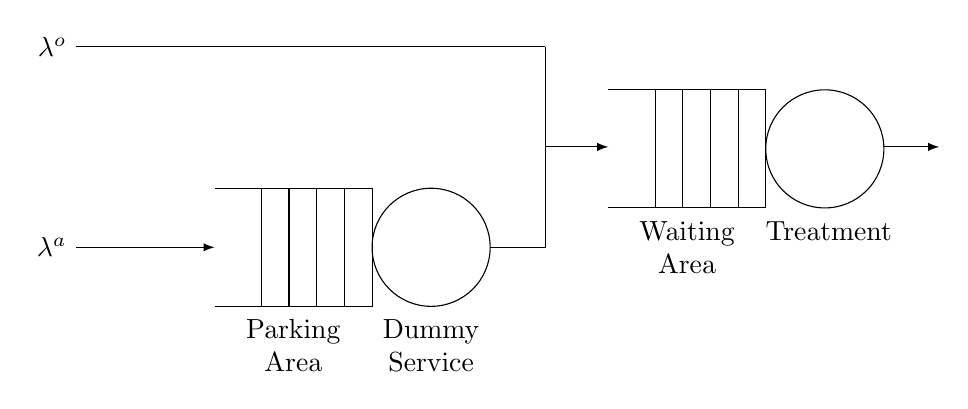
\begin{tikzpicture}[>=latex]
        % the rectangle with vertical rules (Queue 1)
        \draw (0,0) -- ++(2cm,0) -- ++(0,-1.5cm) -- ++(-2cm,0);
        \foreach \i in {1,...,4}
        \draw (2cm-\i*10pt,0) -- +(0,-1.5cm);
        
        % the circle (Queue 1)
        \draw (2.75,-0.75cm) circle [radius=0.75cm];

        % the rectangle with vertical rules (Queue 2)
        \draw (5,1.25) -- ++(2cm,0) -- ++(0,-1.5cm) -- ++(-2cm,0);
        \foreach \i in {1,...,4}
        \draw (7cm-\i*10pt,1.25) -- +(0,-1.5cm);

        % the circle (Queue 2)
        \draw (7.75,0.5) circle [radius=0.75cm];

        % the arrows and labels (Queue 1+2)
        \draw[-] (3.5,-0.75) -- +(20pt,0);
        \draw[<-] (0,-0.75) -- +(-50pt,0) node[left] {\( \lambda^a \)};
        \draw[->] (8.5,0.525) -- +(20pt,0);
        \node[align=center] at (1cm,-2cm) {Parking \\ Area};
        \node[align=center] at (2.75cm,-2cm) {Dummy \\ Service};
        \node[align=center] at (6cm,-0.75cm) {Waiting \\ Area};
        \node[align=center] at (7.8cm,-0.75cm) {Treatment \\ };
        
        \draw (4.2, 1.8) -- +(-169.5pt,0) node[left] {\( \lambda^o \)};
        \draw (4.2, 1.8) -- (4.2, -0.75);
        \draw[->] (4.2, 0.525) -- (5, 0.525);

    \end{tikzpicture}
\end{figure}


\begin{figure}
    \centering
    \begin{tikzpicture}[-, node distance = 1cm, auto, every node/.style={scale=0.5}]

        % Variables
        \tikzmath{
            let \altdist = 1.5cm;
            let \minsz = 1.5cm;
        }

        % First Line
        \node[state, minimum size=1.5cm] (zero) {(0,0)};
        \node[state, minimum size=1.5cm,  right=of zero] (one) {(0,1)};
        \node[draw=none, minimum size=1.5cm, right=of one] (two) {\dots};
        \node[state, minimum size=1.5cm, right=of two] (three) {(0,T)};
        \node[state, node distance = \altdist, minimum size=\minsz, right=of three] (four) {(0,T+1)};
        \node[draw=none, node distance = \altdist, minimum size=\minsz, right=of four] (five) {\dots};
        \node[state, node distance = \altdist, minimum size=\minsz, right=of five] (six) {(0,C)};
        \node[draw=none, minimum size=\minsz, right=of six] (seven) {\dots};

        % Second Line
        \node[state, minimum size=\minsz, below=of three] (three_one) {(1,T)};
        \node[state, minimum size=\minsz, below=of four] (four_one) {(1,T+1)};
        \node[draw=none, minimum size=\minsz, below=of five] (five_one) {\dots};
        \node[state, node distance = \altdist, minimum size=\minsz, right=of five_one] (six_one) {(1,C)};
        \node[draw=none, minimum size=\minsz, right=of six_one] (seven_one) {\dots};

        % Third Line
        \node[state, minimum size=\minsz, below=of three_one] (three_two) {(2,T)};
        \node[state, minimum size=\minsz, below=of four_one] (four_two) {(2,T+1)};
        \node[draw=none, minimum size=\minsz, below=of five_one] (five_two) {\dots};
        \node[state, node distance = \altdist, minimum size=\minsz, right=of five_two] (six_two) {(2,C)};
        \node[draw=none, minimum size=\minsz, right=of six_two] (seven_two) {\dots};

        % Fourth line
        \node[draw=none, minimum size=\minsz, below=of three_two] (three_three) {\vdots};
        \node[draw=none, minimum size=\minsz, below=of four_two] (four_three) {\vdots};
        \node[draw=none, minimum size=\minsz, below=of five_two] (five_three) {};
        \node[draw=none, node distance = \altdist, minimum size=\minsz, right=of five_three] (six_three) {\vdots};

        \draw[every loop]
            % First Horizontal Edges
            (zero) edge[bend left] node {\( \Lambda \)} (one)
            (one) edge[bend left] node [above] {\( \mu \)} (zero)
            (one) edge[bend left] node {\( \Lambda \)} (two)
            (two) edge[bend left] node [above] {\( 2 \mu \)} (one)
            (two) edge[bend left] node {\( \Lambda \)} (three)
            (three) edge[bend left] node [above] {\( T \mu \)} (two)
            (three) edge[bend left] node {\( \lambda^o \)} (four)
            (four) edge[bend left] node [above] {\( (T+1) \mu \)} (three)
            (four) edge[bend left] node {\( \lambda^o \)} (five)
            (five) edge[bend left] node [above] {\( (T+2) \mu \)} (four)
            (five) edge[bend left] node {\( \lambda^o \)} (six)
            (six) edge[bend left] node [above] {\( C\mu \)} (five)
            (six) edge[bend left] node {\( \lambda^o \)} (seven)
            (seven) edge[bend left] node [above] {\( C\mu \)} (six)

            % Second Horizontal Edges
            (three_one) edge[bend left] node {\( \lambda^o \)} (four_one)
            (four_one) edge[bend left] node [above] {\( (T+1) \mu \)} (three_one)
            (four_one) edge[bend left] node {\( \lambda^o \)} (five_one)
            (five_one) edge[bend left] node [above] {\( (T+2) \mu \)} (four_one)
            (five_one) edge[bend left] node {\( \lambda^o \)} (six_one)
            (six_one) edge[bend left] node [above] {\( C\mu \)} (five_one)
            (six_one) edge[bend left] node {\( \lambda^o \)} (seven_one)
            (seven_one) edge[bend left] node [above] {\( C\mu \)} (six_one)

            % Third Horizontal Edges
            (three_two) edge[bend left] node {\( \lambda^o \)} (four_two)
            (four_two) edge[bend left] node [above] {\( (T+1) \mu \)} (three_two)
            (four_two) edge[bend left] node {\( \lambda^o \)} (five_two)
            (five_two) edge[bend left] node [above] {\( (T+2) \mu \)} (four_two)
            (five_two) edge[bend left] node {\( \lambda^o \)} (six_two)
            (six_two) edge[bend left] node [above] {\( C\mu \)} (five_two)
            (six_two) edge[bend left] node {\( \lambda^o \)} (seven_two)
            (seven_two) edge[bend left] node [above] {\( C\mu \)} (six_two)

            % First Vertical Edges
            (three) edge[bend left] node {\( \lambda^A \)} (three_one)
            (three_one) edge[bend left] node {\( T \mu \)} (three)
            (three_one) edge[bend left] node {\( \lambda^A \)} (three_two)
            (three_two) edge[bend left] node {\( T\mu \)} (three_one)
            (three_two) edge[bend left] node {\( \lambda^A \)} (three_three)
            (three_three) edge[bend left] node {\( T\mu \)} (three_two)

            % Second Vertical Edges
            (four) edge node {\( \lambda^A \)} (four_one)
            (four_one) edge node {\( \lambda^A \)} (four_two)
            (four_two) edge node {\( \lambda^A \)} (four_three)

            %Third Vertical Edges
            (six) edge node {\( \lambda^A \)} (six_one)
            (six_one) edge node {\( \lambda^A \)} (six_two)
            (six_two) edge node {\( \lambda^A \)} (six_three)
            ;       
    \end{tikzpicture}
    \caption{Markov chains} 
    \label{Markov_2}
\end{figure}



\begin{figure}
    \centering
    \begin{tikzpicture}[-, node distance = 1cm, auto, every node/.style={scale=0.4}]

        % Variables
        \tikzmath{
            let \altdist = 1cm;
            let \minsz = 1.5cm;
        }

        % First Line
        \node[state, minimum size=1.5cm] (zero) {(0,0)};
        \node[state, minimum size=1.5cm,  right=of zero] (one) {(0,1)};
        \node[draw=none, minimum size=1.5cm, right=of one] (two) {\dots};
        \node[state, minimum size=1.5cm, right=of two] (three) {(0,T)};
        \node[state, node distance = \altdist, minimum size=\minsz, right=of three] (four) {(0,T+1)};
        \node[draw=none, minimum size=\minsz, right=of four] (five) {\dots};
        \node[draw=none, minimum size=\minsz, right=of five] (six) {\vdots};
        \node[draw=none, minimum size=\minsz, right=of six] (seven) {\dots};
        \node[state, minimum size=\minsz, right=of seven] (eight) {(0,C)};
        \node[draw=none, minimum size=\minsz, right=of eight] (nine) {\dots};


        % Second Line
        \node[state, minimum size=\minsz, below=of three] (three_one) {(1,T)};
        \node[state, minimum size=\minsz, below=of four] (four_one) {(1,T+1)};
        \node[draw=none, minimum size=\minsz, below=of five] (five_one) {\dots};
        \node[state, node distance = \altdist, minimum size=\minsz, right=of five_one] (six_one) {\( (u_i, v_i) \)};
        \node[draw=none, minimum size=\minsz, right=of six_one] (seven_one) {\dots};
        \node[state, node distance = \altdist, minimum size=\minsz, right=of seven_one] (eight_one) {(1,C)};
        \node[draw=none, minimum size=\minsz, right=of eight_one] (nine_one) {\dots};
        

        % Third Line
        \node[state, minimum size=\minsz, below=of three_one] (three_two) {(2,T)};
        \node[state, minimum size=\minsz, below=of four_one] (four_two) {(2,T+1)};
        \node[draw=none, minimum size=\minsz, below=of five_one] (five_two) {\dots};
        \node[draw=none, node distance = \altdist, minimum size=\minsz, right=of five_two] (six_two) {\vdots};
        \node[draw=none, minimum size=\minsz, right=of six_two] (seven_two) {\dots};
        \node[state, node distance = \altdist, minimum size=\minsz, right=of seven_two] (eight_two) {(2,C)};
        \node[draw=none, minimum size=\minsz, right=of eight_two] (nine_two) {\dots};

        % Fourth line
        \node[draw=none, minimum size=\minsz, below=of three_two] (three_three) {\vdots};
        \node[draw=none, minimum size=\minsz, below=of four_two] (four_three) {\vdots};
        \node[draw=none, minimum size=\minsz, below=of five_two] (five_three) {};
        \node[draw=none, node distance = \altdist, minimum size=\minsz, right=of five_three] (six_three) {};
        \node[draw=none, node distance = \altdist, minimum size=\minsz, below=of eight_two] (eight_three) {\vdots};


        \draw[every loop]
            % First Horizontal Edges
            (zero) edge[bend left] node {\( \Lambda \)} (one)
            (one) edge[bend left] node {\( \mu \)} (zero)
            (one) edge[bend left] node {\( \Lambda \)} (two)
            (two) edge[bend left] node {\( 2 \mu \)} (one)
            (two) edge[bend left] node {\( \Lambda \)} (three)
            (three) edge[bend left] node {\( T \mu \)} (two)
            (three) edge[bend left] node {\( \lambda^o \)} (four)
            (four) edge[bend left] node {\( (T+1) \mu \)} (three)
            (four) edge[bend left] node {\( \lambda^o \)} (five)
            (five) edge[bend left] node {\( (T+2) \mu \)} (four)
            % (five) edge[bend left] node {\( \lambda^o \)} (six)
            % (six) edge[bend left] node [above] {\( C\mu \)} (five)
            % (six) edge[bend left] node {\( \lambda^o \)} (seven)
            % (seven) edge[bend left] node [above] {\( C\mu \)} (six)
            (seven) edge[bend left] node {\( \lambda^o \)} (eight)
            (eight) edge[bend left] node {\( C\mu \)} (seven)
            (eight) edge[bend left] node {\( \lambda^o \)} (nine)
            (nine) edge[bend left] node {\( C\mu \)} (eight)

            % Second Horizontal Edges
            (three_one) edge[bend left] node {\(\lambda^o\)} (four_one)
            (four_one) edge[bend left] node {\( (T+1) \mu \)} (three_one)
            (four_one) edge[bend left] node {\( \lambda^o \)} (five_one)
            (five_one) edge[bend left] node {\( (T+2) \mu \)} (four_one)
            (five_one) edge[bend left] node {\( \lambda^o \)} (six_one)
            (six_one) edge[bend left] node {\( v_i\mu \)} (five_one)
            (six_one) edge[bend left] node {\( \lambda^o \)} (seven_one)
            (seven_one) edge[bend left] node {\( (v_i+1)\mu \)} (six_one)
            (seven_one) edge[bend left] node {\( \lambda^o \)} (eight_one)
            (eight_one) edge[bend left] node {\( C\mu \)} (seven_one)
            (eight_one) edge[bend left] node {\( \lambda^o \)} (nine_one)
            (nine_one) edge[bend left] node {\( C\mu \)} (eight_one)

            % Third Horizontal Edges
            (three_two) edge[bend left] node {\( \lambda^o \)} (four_two)
            (four_two) edge[bend left] node {\( (T+1) \mu \)} (three_two)
            (four_two) edge[bend left] node {\( \lambda^o \)} (five_two)
            (five_two) edge[bend left] node {\( (T+2) \mu \)} (four_two)
            % (five_two) edge[bend left] node {\( \lambda^o \)} (six_two)
            % (six_two) edge[bend left] node [above] {\( C\mu \)} (five_two)
            % (six_two) edge[bend left] node {\( \lambda^o \)} (seven_two)
            % (seven_two) edge[bend left] node [above] {\( C\mu \)} (six_two)
            (seven_two) edge[bend left] node {\( \lambda^o \)} (eight_two)
            (eight_two) edge[bend left] node {\( C\mu \)} (seven_two)
            (eight_two) edge[bend left] node {\( \lambda^o \)} (nine_two)
            (nine_two) edge[bend left] node {\( C\mu \)} (eight_two)

            % First Vertical Edges
            (three) edge[bend left] node {\( \lambda^A \)} (three_one)
            (three_one) edge[bend left] node {\( T \mu \)} (three)
            (three_one) edge[bend left] node {\( \lambda^A \)} (three_two)
            (three_two) edge[bend left] node {\( T\mu \)} (three_one)
            (three_two) edge[bend left] node {\( \lambda^A \)} (three_three)
            (three_three) edge[bend left] node {\( T\mu \)} (three_two)

            % Second Vertical Edges
            (four) edge node {\( \lambda^A \)} (four_one)
            (four_one) edge node {\( \lambda^A \)} (four_two)
            (four_two) edge node {\( \lambda^A \)} (four_three)

            % Third Vertical Edges
            (six) edge node {\( \lambda^A \)} (six_one)
            (six_one) edge node {\( \lambda^A \)} (six_two)
            % (six_two) edge node {\( \lambda^A \)} (six_three)

            % Fourth Vertical Edges
            (eight) edge node {\( \lambda^A \)} (eight_one)
            (eight_one) edge node {\( \lambda^A \)} (eight_two)
            (eight_two) edge node {\( \lambda^A \)} (eight_three)
            ;       
    \end{tikzpicture}
    \caption{Markov chains} 
    \label{Markov_3}
\end{figure}


\begin{figure}
    \centering
    \begin{tikzpicture}[-, node distance = 0.9cm, auto, every node/.style={scale=0.5}]

        % Variables
        \tikzmath{
            let \initdist = 0.5cm;
            let \altdist = 1.2cm;
            let \minsz = 1.6cm;
            let \leftOne = -0.8;
            let \rightOne = 2.2;
            let \upOne = 0.8;
            let \downOne = -2.2;
            let \leftTwo = 2.25;
            let \rightTwo = 14.2;
            let \upTwo = -2.35;
            let \downTwo = -8.8;
        }

        % % Rectangle for S1
        % \draw[ultra thin, dashed] (\leftOne, \downOne) -- (\leftOne, \upOne);
        % \draw[ultra thin, dashed] (\leftOne, \upOne) -- (\rightOne, \upOne);
        % \draw[ultra thin, dashed] (\rightOne, \upOne) -- node {\Huge{\( \quad S_1 \)}}(\rightOne, \downOne);
        % \draw[ultra thin, dashed] (\rightOne, \downOne) -- (\leftOne, \downOne);

        % % Rectangle for S2
        % \draw[ultra thin, dashed] (\leftTwo, \downTwo) -- node {\Huge{\( S_2 \quad \)}}(\leftTwo, \upTwo);
        % \draw[ultra thin, dashed] (\leftTwo, \upTwo) -- (\rightTwo, \upTwo);
        % \draw[ultra thin, dashed] (\rightTwo, \upTwo) -- (\rightTwo, \downTwo);
        % \draw[ultra thin, dashed] (\rightTwo, \downTwo) -- (\leftTwo, \downTwo);

        % First Line
        \node[state, minimum size=1.5cm] (zero) {(0,0)};
        \node[state, node distance = \initdist, minimum size=\minsz, below right=of zero] (one) {(0,1)};
        \node[draw=none, node distance = \initdist, minimum size=\minsz, below right=of one] (two) {\textbf{\( \ddots \)}};
        \node[state, node distance = \initdist, minimum size=\minsz, below right=of two] (three) {(0,T)};
        \node[state, node distance = \altdist, minimum size=\minsz, right=of three] (four) {(0,T+1)};
        \node[draw=none, node distance = \altdist, minimum size=\minsz, right=of four] (five) {\textbf{\dots}};
        \node[draw=none, minimum size=\minsz, right=of five] (six) {\textbf{\vdots}};
        \node[draw=none, minimum size=\minsz, right=of six] (seven) {\textbf{\dots}};
        \node[state, minimum size=\minsz, right=of seven] (eight) {(0,C)};
        \node[draw=none, minimum size=\minsz, right=of eight] (nine) {\textbf{\dots}};


        % Second Line
        \node[state, minimum size=\minsz, below=of three] (three_one) {(1,T)};
        \node[state, minimum size=\minsz, below=of four] (four_one) {(1,T+1)};
        \node[draw=none, minimum size=\minsz, below=of five] (five_one) {\textbf{\dots}};
        \node[state, minimum size=\minsz, right=of five_one] (six_one) {\( (u_i, v_i) \)};
        \node[draw=none, minimum size=\minsz, right=of six_one] (seven_one) {\textbf{\dots}};
        \node[state, minimum size=\minsz, right=of seven_one] (eight_one) {(1,C)};
        \node[draw=none, minimum size=\minsz, right=of eight_one] (nine_one) {\textbf{\dots}};
        

        % Third Line
        \node[state, minimum size=\minsz, below=of three_one] (three_two) {(2,T)};
        \node[state, minimum size=\minsz, below=of four_one] (four_two) {(2,T+1)};
        \node[draw=none, minimum size=\minsz, below=of five_one] (five_two) {\textbf{\dots}};
        \node[draw=none, minimum size=\minsz, right=of five_two] (six_two) {\textbf{\vdots}};
        \node[draw=none, minimum size=\minsz, right=of six_two] (seven_two) {\textbf{\dots}};
        \node[state, minimum size=\minsz, right=of seven_two] (eight_two) {(2,C)};
        \node[draw=none, minimum size=\minsz, right=of eight_two] (nine_two) {\textbf{\dots}};

        % Fourth line
        \node[draw=none, node distance = \altdist, minimum size=\minsz, below=of three_two] (three_three) {\textbf{\vdots}};
        \node[draw=none, node distance = \altdist, minimum size=\minsz, below=of four_two] (four_three) {\textbf{\vdots}};
        \node[draw=none, node distance = \altdist, minimum size=\minsz, below=of five_two] (five_three) {};
        \node[draw=none, node distance = \altdist, minimum size=\minsz, below=of six_two] (six_three) {};
        \node[draw=none, node distance = \altdist, minimum size=\minsz, below=of eight_two] (eight_three) {\textbf{\vdots}};


        \draw[every loop]
            % First Horizontal Edges
            (zero) edge[bend left] node {\( \Lambda \)} (one)
            (one) edge[bend left] node {\( \mu \)} (zero)
            (one) edge[bend left] node {\( \Lambda \)} (two)
            (two) edge[bend left] node {\( 2 \mu \)} (one)
            (two) edge[bend left] node {\( \Lambda \)} (three)
            (three) edge[bend left] node {\( T \mu \)} (two)
            (three) edge[bend left] node {\( \lambda^o \)} (four)
            (four) edge[bend left] node {\( (T+1) \mu \)} (three)
            (four) edge[bend left] node {\( \lambda^o \)} (five)
            (five) edge[bend left] node {\( (T+2) \mu \)} (four)
            % (five) edge[bend left] node {\( \lambda^o \)} (six)
            % (six) edge[bend left] node [above] {\( C\mu \)} (five)
            % (six) edge[bend left] node {\( \lambda^o \)} (seven)
            % (seven) edge[bend left] node [above] {\( C\mu \)} (six)
            (seven) edge[bend left] node {\( \lambda^o \)} (eight)
            (eight) edge[bend left] node {\( C\mu \)} (seven)
            (eight) edge[bend left] node {\( \lambda^o \)} (nine)
            (nine) edge[bend left] node {\( C\mu \)} (eight)

            % Second Horizontal Edges
            (three_one) edge[bend left] node {\( \lambda^o \)} (four_one)
            (four_one) edge[bend left] node {\( (T+1) \mu \)} (three_one)
            (four_one) edge[bend left] node {\( \lambda^o \)} (five_one)
            (five_one) edge[bend left] node {\( (T+2) \mu \)} (four_one)
            (five_one) edge[bend left] node {\( \lambda^o \)} (six_one)
            (six_one) edge[bend left] node {\( v_i\mu \)} (five_one)
            (six_one) edge[bend left] node {\( \lambda^o \)} (seven_one)
            (seven_one) edge[bend left] node {\( (v_i+1)\mu \)} (six_one)
            (seven_one) edge[bend left] node {\( \lambda^o \)} (eight_one)
            (eight_one) edge[bend left] node {\( C\mu \)} (seven_one)
            (eight_one) edge[bend left] node {\( \lambda^o \)} (nine_one)
            (nine_one) edge[bend left] node {\( C\mu \)} (eight_one)

            % Third Horizontal Edges
            (three_two) edge[bend left] node {\( \lambda^o \)} (four_two)
            (four_two) edge[bend left] node [below] {\( (T+1) \mu \)} (three_two)
            (four_two) edge[bend left] node {\( \lambda^o \)} (five_two)
            (five_two) edge[bend left] node {\( (T+2) \mu \)} (four_two)
            % (five_two) edge[bend left] node {\( \lambda^o \)} (six_two)
            % (six_two) edge[bend left] node [above] {\( C\mu \)} (five_two)
            % (six_two) edge[bend left] node {\( \lambda^o \)} (seven_two)
            % (seven_two) edge[bend left] node [above] {\( C\mu \)} (six_two)
            (seven_two) edge[bend left] node {\( \lambda^o \)} (eight_two)
            (eight_two) edge[bend left] node {\( C\mu \)} (seven_two)
            (eight_two) edge[bend left] node {\( \lambda^o \)} (nine_two)
            (nine_two) edge[bend left] node {\( C\mu \)} (eight_two)

            % First Vertical Edges
            (three) edge[bend left] node {\( \lambda^A \)} (three_one)
            (three_one) edge[bend left] node {\( T \mu \)} (three)
            (three_one) edge[bend left] node {\( \lambda^A \)} (three_two)
            (three_two) edge[bend left] node {\( T\mu \)} (three_one)
            (three_two) edge[bend left] node {\( \lambda^A \)} (three_three)
            (three_three) edge[bend left] node {\( T\mu \)} (three_two)

            % Second Vertical Edges
            (four) edge node {\( \lambda^A \)} (four_one)
            (four_one) edge node {\( \lambda^A \)} (four_two)
            (four_two) edge node {\( \lambda^A \)} (four_three)

            % Third Vertical Edges
            (six) edge node {\( \lambda^A \)} (six_one)
            (six_one) edge node {\( \lambda^A \)} (six_two)
            % (six_two) edge node {\( \lambda^A \)} (six_three)

            % Fourth Vertical Edges
            (eight) edge node {\( \lambda^A \)} (eight_one)
            (eight_one) edge node {\( \lambda^A \)} (eight_two)
            (eight_two) edge node {\( \lambda^A \)} (eight_three)
            ;       
    \end{tikzpicture}
    \caption{Markov chains} 
    \label{Markov_4}
\end{figure}




\begin{figure}
    \centering
    \begin{tikzpicture}[-, node distance = 0.9cm, auto, every node/.style={scale=0.7}]

        % Markov chain variables
        \tikzmath{
            let \initdist = 0.5cm;
            let \altdist = 1.2cm;
            let \minsz = 1.6cm;
        }

        % S_1 and S_2 rectangles
        \tikzmath{
            let \leftOne = -0.8;
            let \rightOne = 2.7;
            let \upOne = 0.8;
            let \downOne = -2.7;
            let \leftTwo = 2.8;
            let \rightTwo = 13;
            let \upTwo = -2.95;
            let \downTwo = -16.4;
        }

        % General case variables
        \tikzmath{
            let \GCsmallx = 8.3;
            let \GCsmally = -9.5;
            let \GCbigx = 4.1;
            let \GCbigy = -11.8;
        }

        % % Rectangle for S1
        % \draw[ultra thin, dashed] (\leftOne, \downOne) -- (\leftOne, \upOne);
        % \draw[ultra thin, dashed] (\leftOne, \upOne) -- (\rightOne, \upOne);
        % \draw[ultra thin, dashed] (\rightOne, \upOne) -- node {\Huge{\( \quad S_1 \)}}(\rightOne, \downOne);
        % \draw[ultra thin, dashed] (\rightOne, \downOne) -- (\leftOne, \downOne);

        % % Rectangle for S2
        % \draw[ultra thin, dashed] (\leftTwo, \downTwo) -- node {\Huge{\( S_2 \quad \)}}(\leftTwo, \upTwo);
        % \draw[ultra thin, dashed] (\leftTwo, \upTwo) -- (\rightTwo, \upTwo);
        % \draw[ultra thin, dashed] (\rightTwo, \upTwo) -- (\rightTwo, \downTwo);
        % \draw[ultra thin, dashed] (\rightTwo, \downTwo) -- (\leftTwo, \downTwo);

        % Small square of general case
        \draw [thick] (\GCsmallx, \GCsmally) -- node {} (\GCsmallx + 0.4, \GCsmally);
        \draw [thick] (\GCsmallx + 0.4, \GCsmally) -- node {} (\GCsmallx + 0.4, \GCsmally - 0.4);
        \draw [thick] (\GCsmallx + 0.4, \GCsmally - 0.4) -- node {} (\GCsmallx, \GCsmally - 0.4);
        \draw [thick] (\GCsmallx, \GCsmally - 0.4) -- node {} (\GCsmallx, \GCsmally);


        % Dashed lines to from small square to big one 
        \draw [ultra thin] (\GCsmallx, \GCsmally) -- node {} (\GCbigx, \GCbigy);
        \draw [ultra thin] (\GCsmallx + 0.4, \GCsmally) -- node {} (\GCbigx + 4, \GCbigy);
        \draw [ultra thin] (\GCsmallx, \GCsmally - 0.4) -- node {} (7, \GCbigy);
        \draw [ultra thin] (\GCsmallx + 0.4, \GCsmally - 0.4) -- node {} (\GCbigx + 4, \GCbigy - 4);
        
        % Big Square of general case
        \draw [ultra thick] (\GCbigx, \GCbigy) -- node {} (\GCbigx + 4, \GCbigy);
        \draw [ultra thick] (\GCbigx + 4, \GCbigy) -- node {} (\GCbigx + 4, \GCbigy - 4);
        \draw [ultra thick] (\GCbigx + 4, \GCbigy - 4) -- node {General Case} (\GCbigx, \GCbigy - 4);
        \draw [ultra thick] (\GCbigx, \GCbigy - 4) -- node {} (\GCbigx, \GCbigy);

        % First Line
        \node[state, minimum size=1.5cm] (zero) {(0,0)};
        \node[state, node distance = \initdist, minimum size=\minsz, below right=of zero] (one) {(0,1)};
        \node[draw=none, node distance = \initdist, minimum size=\minsz, below right=of one] (two) {\textbf{\( \ddots \)}};
        \node[state, node distance = \initdist, minimum size=\minsz, below right=of two] (three) {(0,T)};
        \node[state, node distance = \altdist, minimum size=\minsz, right=of three] (four) {(0,T+1)};
        \node[draw=none, node distance = \altdist, minimum size=\minsz, right=of four] (five) {\textbf{\dots}};
        \node[state, minimum size=\minsz, right=of five] (six) {(0,C)};
        \node[draw=none, minimum size=\minsz, right=of six] (seven) {\textbf{\dots}};

        % Second Line
        \node[state, minimum size=\minsz, below=of three] (three_one) {(1,T)};
        \node[state, minimum size=\minsz, below=of four] (four_one) {(1,T+1)};
        \node[draw=none, minimum size=\minsz, below=of five] (five_one) {\textbf{\dots}};
        \node[state, minimum size=\minsz, right=of five_one] (six_one) {(1,C)};
        \node[draw=none, minimum size=\minsz, right=of six_one] (seven_one) {\textbf{\dots}};
        
        % Third Line
        \node[state, minimum size=\minsz, below=of three_one] (three_two) {(2,T)};
        \node[state, minimum size=\minsz, below=of four_one] (four_two) {(2,T+1)};
        \node[draw=none, minimum size=\minsz, below=of five_one] (five_two) {\textbf{\dots}};
        \node[state, minimum size=\minsz, right=of five_two] (six_two) {(2,C)};
        \node[draw=none, minimum size=\minsz, right=of six_two] (seven_two) {\textbf{\dots}};

        % Fourth line
        \node[draw=none, node distance = \altdist, minimum size=\minsz, below=of three_two] (three_three) {\textbf{\vdots}};
        \node[draw=none, node distance = \altdist, minimum size=\minsz, below=of four_two] (four_three) {\textbf{\vdots}};
        \node[draw=none, node distance = 2cm, minimum size=\minsz, below=of five_two] (five_three) {};
        \node[draw=none, node distance = \altdist, minimum size=\minsz, below=of six_two] (six_three) {\textbf{\vdots}};

        % Fifth line
        % \node[state, node distance = \altdist, minimum size=\minsz, below=of five_three] (general_case_mid) {\( (u_i, v_i) \)};
        \node[draw=none, node distance = 0.3cm, minimum size=\minsz, below=of four_three] (general_case_up) {};
        \node[state, node distance = \altdist, minimum size=\minsz, below=of general_case_up] (general_case_mid) {\( (u_i, v_i) \)};

        \node[draw=none, node distance = \altdist, minimum size=\minsz, below=of general_case_mid] (general_case_down) {};
        \node[draw=none, node distance = \altdist, minimum size=\minsz, left=of general_case_mid] (general_case_left) {};
        \node[draw=none, node distance = \altdist, minimum size=\minsz, right=of general_case_mid] (general_case_right) {};

        \draw[every loop]
            % First Horizontal Edges
            (zero) edge[bend left] node {\( \Lambda \)} (one)
            (one) edge[bend left] node {\( \mu \)} (zero)
            (one) edge[bend left] node {\( \Lambda \)} (two)
            (two) edge[bend left] node {\( 2 \mu \)} (one)
            (two) edge[bend left] node {\( \Lambda \)} (three)
            (three) edge[bend left] node {\( T \mu \)} (two)
            (three) edge[bend left] node {\( \lambda^o \)} (four)
            (four) edge[bend left] node {\( (T+1) \mu \)} (three)
            (four) edge[bend left] node {\( \lambda^o \)} (five)
            (five) edge[bend left] node {\( (T+2) \mu \)} (four)
            (five) edge[bend left] node {\( \lambda^o \)} (six)
            (six) edge[bend left] node {\( C\mu \)} (five)
            (six) edge[bend left] node {\( \lambda^o \)} (seven)
            (seven) edge[bend left] node {\( C\mu \)} (six)

            % Second Horizontal Edges
            (three_one) edge[bend left] node {\( \lambda^o \)} (four_one)
            (four_one) edge[bend left] node {\( (T+1) \mu \)} (three_one)
            (four_one) edge[bend left] node {\( \lambda^o \)} (five_one)
            (five_one) edge[bend left] node {\( (T+2) \mu \)} (four_one)
            (five_one) edge[bend left] node {\( \lambda^o \)} (six_one)
            (six_one) edge[bend left] node {\( C\mu \)} (five_one)
            (six_one) edge[bend left] node {\( \lambda^o \)} (seven_one)
            (seven_one) edge[bend left] node {\( C\mu \)} (six_one)

            % Third Horizontal Edges
            (three_two) edge[bend left] node {\( \lambda^o \)} (four_two)
            (four_two) edge[bend left] node [below] {\( (T+1) \mu \)} (three_two)
            (four_two) edge[bend left] node {\( \lambda^o \)} (five_two)
            (five_two) edge[bend left] node {\( (T+2) \mu \)} (four_two)
            (five_two) edge[bend left] node {\( \lambda^o \)} (six_two)
            (six_two) edge[bend left] node {\( C\mu \)} (five_two)
            (six_two) edge[bend left] node {\( \lambda^o \)} (seven_two)
            (seven_two) edge[bend left] node {\( C\mu \)} (six_two)

            % First Vertical Edges
            (three) edge[bend left] node {\( \lambda^A \)} (three_one)
            (three_one) edge[bend left] node {\( T \mu \)} (three)
            (three_one) edge[bend left] node {\( \lambda^A \)} (three_two)
            (three_two) edge[bend left] node {\( T\mu \)} (three_one)
            (three_two) edge[bend left] node {\( \lambda^A \)} (three_three)
            (three_three) edge[bend left] node {\( T\mu \)} (three_two)

            % Second Vertical Edges
            (four) edge node {\( \lambda^A \)} (four_one)
            (four_one) edge node {\( \lambda^A \)} (four_two)
            (four_two) edge node {\( \lambda^A \)} (four_three)

            % Fourth Vertical Edges
            (six) edge node {\( \lambda^A \)} (six_one)
            (six_one) edge node {\( \lambda^A \)} (six_two)
            (six_two) edge node {\( \lambda^A \)} (six_three)

            % General Case
            (general_case_left) edge[bend left] node {\( \lambda^o \)} (general_case_mid)
            (general_case_mid) edge[bend left] node {\( v_i \mu \)} (general_case_left)
            (general_case_right) edge[bend left] node {\( (v_i +1) \mu \)} (general_case_mid)
            (general_case_mid) edge[bend left] node {\( \lambda_o \)} (general_case_right)
            % (five_three) edge node {\( \lambda_A \)} (general_case_mid)
            (general_case_up) edge node {\( \lambda_A \)} (general_case_mid)
            (general_case_mid) edge node {\( \lambda_A \)} (general_case_down)
            ;
    \end{tikzpicture}
    \caption{Markov chain} 
    \label{Markov_5}
\end{figure}

}
    \end{figure}
    \columnbreak
    \begin{figure}[H]
        \centering
        \scalebox{0.9}{
            \section{Figures that might be useful}
\begin{figure}[h]
    \centering
    \begin{tikzpicture}[>=latex]
        % the rectangle with vertical rules (Queue 1)
        \draw (0,0) -- ++(2cm,0) -- ++(0,-1.5cm) -- ++(-2cm,0);
        \foreach \i in {1,...,4}
        \draw (2cm-\i*10pt,0) -- +(0,-1.5cm);
        
        % the circle (Queue 1)
        \draw (2.75,-0.75cm) circle [radius=0.75cm];

        % the rectangle with vertical rules (Queue 2)
        \draw (5,1.25) -- ++(2cm,0) -- ++(0,-1.5cm) -- ++(-2cm,0);
        \foreach \i in {1,...,4}
        \draw (7cm-\i*10pt,1.25) -- +(0,-1.5cm);

        % the circle (Queue 2)
        \draw (7.75,0.5) circle [radius=0.75cm];

        % the arrows and labels (Queue 1+2)
        \draw[-] (3.5,-0.75) -- +(20pt,0);
        \draw[<-] (0,-0.75) -- +(-50pt,0) node[left] {\( \lambda^a \)};
        \draw[->] (8.5,0.525) -- +(20pt,0);
        \node[align=center] at (1cm,-2cm) {Parking \\ Area};
        \node[align=center] at (2.75cm,-2cm) {Dummy \\ Service};
        \node[align=center] at (6cm,-0.75cm) {Waiting \\ Area};
        \node[align=center] at (7.8cm,-0.75cm) {Treatment \\ };
        
        \draw (4.2, 1.8) -- +(-169.5pt,0) node[left] {\( \lambda^o \)};
        \draw (4.2, 1.8) -- (4.2, -0.75);
        \draw[->] (4.2, 0.525) -- (5, 0.525);

    \end{tikzpicture}
\end{figure}


\begin{figure}
    \centering
    \begin{tikzpicture}[-, node distance = 1cm, auto, every node/.style={scale=0.5}]

        % Variables
        \tikzmath{
            let \altdist = 1.5cm;
            let \minsz = 1.5cm;
        }

        % First Line
        \node[state, minimum size=1.5cm] (zero) {(0,0)};
        \node[state, minimum size=1.5cm,  right=of zero] (one) {(0,1)};
        \node[draw=none, minimum size=1.5cm, right=of one] (two) {\dots};
        \node[state, minimum size=1.5cm, right=of two] (three) {(0,T)};
        \node[state, node distance = \altdist, minimum size=\minsz, right=of three] (four) {(0,T+1)};
        \node[draw=none, node distance = \altdist, minimum size=\minsz, right=of four] (five) {\dots};
        \node[state, node distance = \altdist, minimum size=\minsz, right=of five] (six) {(0,C)};
        \node[draw=none, minimum size=\minsz, right=of six] (seven) {\dots};

        % Second Line
        \node[state, minimum size=\minsz, below=of three] (three_one) {(1,T)};
        \node[state, minimum size=\minsz, below=of four] (four_one) {(1,T+1)};
        \node[draw=none, minimum size=\minsz, below=of five] (five_one) {\dots};
        \node[state, node distance = \altdist, minimum size=\minsz, right=of five_one] (six_one) {(1,C)};
        \node[draw=none, minimum size=\minsz, right=of six_one] (seven_one) {\dots};

        % Third Line
        \node[state, minimum size=\minsz, below=of three_one] (three_two) {(2,T)};
        \node[state, minimum size=\minsz, below=of four_one] (four_two) {(2,T+1)};
        \node[draw=none, minimum size=\minsz, below=of five_one] (five_two) {\dots};
        \node[state, node distance = \altdist, minimum size=\minsz, right=of five_two] (six_two) {(2,C)};
        \node[draw=none, minimum size=\minsz, right=of six_two] (seven_two) {\dots};

        % Fourth line
        \node[draw=none, minimum size=\minsz, below=of three_two] (three_three) {\vdots};
        \node[draw=none, minimum size=\minsz, below=of four_two] (four_three) {\vdots};
        \node[draw=none, minimum size=\minsz, below=of five_two] (five_three) {};
        \node[draw=none, node distance = \altdist, minimum size=\minsz, right=of five_three] (six_three) {\vdots};

        \draw[every loop]
            % First Horizontal Edges
            (zero) edge[bend left] node {\( \Lambda \)} (one)
            (one) edge[bend left] node [above] {\( \mu \)} (zero)
            (one) edge[bend left] node {\( \Lambda \)} (two)
            (two) edge[bend left] node [above] {\( 2 \mu \)} (one)
            (two) edge[bend left] node {\( \Lambda \)} (three)
            (three) edge[bend left] node [above] {\( T \mu \)} (two)
            (three) edge[bend left] node {\( \lambda^o \)} (four)
            (four) edge[bend left] node [above] {\( (T+1) \mu \)} (three)
            (four) edge[bend left] node {\( \lambda^o \)} (five)
            (five) edge[bend left] node [above] {\( (T+2) \mu \)} (four)
            (five) edge[bend left] node {\( \lambda^o \)} (six)
            (six) edge[bend left] node [above] {\( C\mu \)} (five)
            (six) edge[bend left] node {\( \lambda^o \)} (seven)
            (seven) edge[bend left] node [above] {\( C\mu \)} (six)

            % Second Horizontal Edges
            (three_one) edge[bend left] node {\( \lambda^o \)} (four_one)
            (four_one) edge[bend left] node [above] {\( (T+1) \mu \)} (three_one)
            (four_one) edge[bend left] node {\( \lambda^o \)} (five_one)
            (five_one) edge[bend left] node [above] {\( (T+2) \mu \)} (four_one)
            (five_one) edge[bend left] node {\( \lambda^o \)} (six_one)
            (six_one) edge[bend left] node [above] {\( C\mu \)} (five_one)
            (six_one) edge[bend left] node {\( \lambda^o \)} (seven_one)
            (seven_one) edge[bend left] node [above] {\( C\mu \)} (six_one)

            % Third Horizontal Edges
            (three_two) edge[bend left] node {\( \lambda^o \)} (four_two)
            (four_two) edge[bend left] node [above] {\( (T+1) \mu \)} (three_two)
            (four_two) edge[bend left] node {\( \lambda^o \)} (five_two)
            (five_two) edge[bend left] node [above] {\( (T+2) \mu \)} (four_two)
            (five_two) edge[bend left] node {\( \lambda^o \)} (six_two)
            (six_two) edge[bend left] node [above] {\( C\mu \)} (five_two)
            (six_two) edge[bend left] node {\( \lambda^o \)} (seven_two)
            (seven_two) edge[bend left] node [above] {\( C\mu \)} (six_two)

            % First Vertical Edges
            (three) edge[bend left] node {\( \lambda^A \)} (three_one)
            (three_one) edge[bend left] node {\( T \mu \)} (three)
            (three_one) edge[bend left] node {\( \lambda^A \)} (three_two)
            (three_two) edge[bend left] node {\( T\mu \)} (three_one)
            (three_two) edge[bend left] node {\( \lambda^A \)} (three_three)
            (three_three) edge[bend left] node {\( T\mu \)} (three_two)

            % Second Vertical Edges
            (four) edge node {\( \lambda^A \)} (four_one)
            (four_one) edge node {\( \lambda^A \)} (four_two)
            (four_two) edge node {\( \lambda^A \)} (four_three)

            %Third Vertical Edges
            (six) edge node {\( \lambda^A \)} (six_one)
            (six_one) edge node {\( \lambda^A \)} (six_two)
            (six_two) edge node {\( \lambda^A \)} (six_three)
            ;       
    \end{tikzpicture}
    \caption{Markov chains} 
    \label{Markov_2}
\end{figure}



\begin{figure}
    \centering
    \begin{tikzpicture}[-, node distance = 1cm, auto, every node/.style={scale=0.4}]

        % Variables
        \tikzmath{
            let \altdist = 1cm;
            let \minsz = 1.5cm;
        }

        % First Line
        \node[state, minimum size=1.5cm] (zero) {(0,0)};
        \node[state, minimum size=1.5cm,  right=of zero] (one) {(0,1)};
        \node[draw=none, minimum size=1.5cm, right=of one] (two) {\dots};
        \node[state, minimum size=1.5cm, right=of two] (three) {(0,T)};
        \node[state, node distance = \altdist, minimum size=\minsz, right=of three] (four) {(0,T+1)};
        \node[draw=none, minimum size=\minsz, right=of four] (five) {\dots};
        \node[draw=none, minimum size=\minsz, right=of five] (six) {\vdots};
        \node[draw=none, minimum size=\minsz, right=of six] (seven) {\dots};
        \node[state, minimum size=\minsz, right=of seven] (eight) {(0,C)};
        \node[draw=none, minimum size=\minsz, right=of eight] (nine) {\dots};


        % Second Line
        \node[state, minimum size=\minsz, below=of three] (three_one) {(1,T)};
        \node[state, minimum size=\minsz, below=of four] (four_one) {(1,T+1)};
        \node[draw=none, minimum size=\minsz, below=of five] (five_one) {\dots};
        \node[state, node distance = \altdist, minimum size=\minsz, right=of five_one] (six_one) {\( (u_i, v_i) \)};
        \node[draw=none, minimum size=\minsz, right=of six_one] (seven_one) {\dots};
        \node[state, node distance = \altdist, minimum size=\minsz, right=of seven_one] (eight_one) {(1,C)};
        \node[draw=none, minimum size=\minsz, right=of eight_one] (nine_one) {\dots};
        

        % Third Line
        \node[state, minimum size=\minsz, below=of three_one] (three_two) {(2,T)};
        \node[state, minimum size=\minsz, below=of four_one] (four_two) {(2,T+1)};
        \node[draw=none, minimum size=\minsz, below=of five_one] (five_two) {\dots};
        \node[draw=none, node distance = \altdist, minimum size=\minsz, right=of five_two] (six_two) {\vdots};
        \node[draw=none, minimum size=\minsz, right=of six_two] (seven_two) {\dots};
        \node[state, node distance = \altdist, minimum size=\minsz, right=of seven_two] (eight_two) {(2,C)};
        \node[draw=none, minimum size=\minsz, right=of eight_two] (nine_two) {\dots};

        % Fourth line
        \node[draw=none, minimum size=\minsz, below=of three_two] (three_three) {\vdots};
        \node[draw=none, minimum size=\minsz, below=of four_two] (four_three) {\vdots};
        \node[draw=none, minimum size=\minsz, below=of five_two] (five_three) {};
        \node[draw=none, node distance = \altdist, minimum size=\minsz, right=of five_three] (six_three) {};
        \node[draw=none, node distance = \altdist, minimum size=\minsz, below=of eight_two] (eight_three) {\vdots};


        \draw[every loop]
            % First Horizontal Edges
            (zero) edge[bend left] node {\( \Lambda \)} (one)
            (one) edge[bend left] node {\( \mu \)} (zero)
            (one) edge[bend left] node {\( \Lambda \)} (two)
            (two) edge[bend left] node {\( 2 \mu \)} (one)
            (two) edge[bend left] node {\( \Lambda \)} (three)
            (three) edge[bend left] node {\( T \mu \)} (two)
            (three) edge[bend left] node {\( \lambda^o \)} (four)
            (four) edge[bend left] node {\( (T+1) \mu \)} (three)
            (four) edge[bend left] node {\( \lambda^o \)} (five)
            (five) edge[bend left] node {\( (T+2) \mu \)} (four)
            % (five) edge[bend left] node {\( \lambda^o \)} (six)
            % (six) edge[bend left] node [above] {\( C\mu \)} (five)
            % (six) edge[bend left] node {\( \lambda^o \)} (seven)
            % (seven) edge[bend left] node [above] {\( C\mu \)} (six)
            (seven) edge[bend left] node {\( \lambda^o \)} (eight)
            (eight) edge[bend left] node {\( C\mu \)} (seven)
            (eight) edge[bend left] node {\( \lambda^o \)} (nine)
            (nine) edge[bend left] node {\( C\mu \)} (eight)

            % Second Horizontal Edges
            (three_one) edge[bend left] node {\(\lambda^o\)} (four_one)
            (four_one) edge[bend left] node {\( (T+1) \mu \)} (three_one)
            (four_one) edge[bend left] node {\( \lambda^o \)} (five_one)
            (five_one) edge[bend left] node {\( (T+2) \mu \)} (four_one)
            (five_one) edge[bend left] node {\( \lambda^o \)} (six_one)
            (six_one) edge[bend left] node {\( v_i\mu \)} (five_one)
            (six_one) edge[bend left] node {\( \lambda^o \)} (seven_one)
            (seven_one) edge[bend left] node {\( (v_i+1)\mu \)} (six_one)
            (seven_one) edge[bend left] node {\( \lambda^o \)} (eight_one)
            (eight_one) edge[bend left] node {\( C\mu \)} (seven_one)
            (eight_one) edge[bend left] node {\( \lambda^o \)} (nine_one)
            (nine_one) edge[bend left] node {\( C\mu \)} (eight_one)

            % Third Horizontal Edges
            (three_two) edge[bend left] node {\( \lambda^o \)} (four_two)
            (four_two) edge[bend left] node {\( (T+1) \mu \)} (three_two)
            (four_two) edge[bend left] node {\( \lambda^o \)} (five_two)
            (five_two) edge[bend left] node {\( (T+2) \mu \)} (four_two)
            % (five_two) edge[bend left] node {\( \lambda^o \)} (six_two)
            % (six_two) edge[bend left] node [above] {\( C\mu \)} (five_two)
            % (six_two) edge[bend left] node {\( \lambda^o \)} (seven_two)
            % (seven_two) edge[bend left] node [above] {\( C\mu \)} (six_two)
            (seven_two) edge[bend left] node {\( \lambda^o \)} (eight_two)
            (eight_two) edge[bend left] node {\( C\mu \)} (seven_two)
            (eight_two) edge[bend left] node {\( \lambda^o \)} (nine_two)
            (nine_two) edge[bend left] node {\( C\mu \)} (eight_two)

            % First Vertical Edges
            (three) edge[bend left] node {\( \lambda^A \)} (three_one)
            (three_one) edge[bend left] node {\( T \mu \)} (three)
            (three_one) edge[bend left] node {\( \lambda^A \)} (three_two)
            (three_two) edge[bend left] node {\( T\mu \)} (three_one)
            (three_two) edge[bend left] node {\( \lambda^A \)} (three_three)
            (three_three) edge[bend left] node {\( T\mu \)} (three_two)

            % Second Vertical Edges
            (four) edge node {\( \lambda^A \)} (four_one)
            (four_one) edge node {\( \lambda^A \)} (four_two)
            (four_two) edge node {\( \lambda^A \)} (four_three)

            % Third Vertical Edges
            (six) edge node {\( \lambda^A \)} (six_one)
            (six_one) edge node {\( \lambda^A \)} (six_two)
            % (six_two) edge node {\( \lambda^A \)} (six_three)

            % Fourth Vertical Edges
            (eight) edge node {\( \lambda^A \)} (eight_one)
            (eight_one) edge node {\( \lambda^A \)} (eight_two)
            (eight_two) edge node {\( \lambda^A \)} (eight_three)
            ;       
    \end{tikzpicture}
    \caption{Markov chains} 
    \label{Markov_3}
\end{figure}


\begin{figure}
    \centering
    \begin{tikzpicture}[-, node distance = 0.9cm, auto, every node/.style={scale=0.5}]

        % Variables
        \tikzmath{
            let \initdist = 0.5cm;
            let \altdist = 1.2cm;
            let \minsz = 1.6cm;
            let \leftOne = -0.8;
            let \rightOne = 2.2;
            let \upOne = 0.8;
            let \downOne = -2.2;
            let \leftTwo = 2.25;
            let \rightTwo = 14.2;
            let \upTwo = -2.35;
            let \downTwo = -8.8;
        }

        % % Rectangle for S1
        % \draw[ultra thin, dashed] (\leftOne, \downOne) -- (\leftOne, \upOne);
        % \draw[ultra thin, dashed] (\leftOne, \upOne) -- (\rightOne, \upOne);
        % \draw[ultra thin, dashed] (\rightOne, \upOne) -- node {\Huge{\( \quad S_1 \)}}(\rightOne, \downOne);
        % \draw[ultra thin, dashed] (\rightOne, \downOne) -- (\leftOne, \downOne);

        % % Rectangle for S2
        % \draw[ultra thin, dashed] (\leftTwo, \downTwo) -- node {\Huge{\( S_2 \quad \)}}(\leftTwo, \upTwo);
        % \draw[ultra thin, dashed] (\leftTwo, \upTwo) -- (\rightTwo, \upTwo);
        % \draw[ultra thin, dashed] (\rightTwo, \upTwo) -- (\rightTwo, \downTwo);
        % \draw[ultra thin, dashed] (\rightTwo, \downTwo) -- (\leftTwo, \downTwo);

        % First Line
        \node[state, minimum size=1.5cm] (zero) {(0,0)};
        \node[state, node distance = \initdist, minimum size=\minsz, below right=of zero] (one) {(0,1)};
        \node[draw=none, node distance = \initdist, minimum size=\minsz, below right=of one] (two) {\textbf{\( \ddots \)}};
        \node[state, node distance = \initdist, minimum size=\minsz, below right=of two] (three) {(0,T)};
        \node[state, node distance = \altdist, minimum size=\minsz, right=of three] (four) {(0,T+1)};
        \node[draw=none, node distance = \altdist, minimum size=\minsz, right=of four] (five) {\textbf{\dots}};
        \node[draw=none, minimum size=\minsz, right=of five] (six) {\textbf{\vdots}};
        \node[draw=none, minimum size=\minsz, right=of six] (seven) {\textbf{\dots}};
        \node[state, minimum size=\minsz, right=of seven] (eight) {(0,C)};
        \node[draw=none, minimum size=\minsz, right=of eight] (nine) {\textbf{\dots}};


        % Second Line
        \node[state, minimum size=\minsz, below=of three] (three_one) {(1,T)};
        \node[state, minimum size=\minsz, below=of four] (four_one) {(1,T+1)};
        \node[draw=none, minimum size=\minsz, below=of five] (five_one) {\textbf{\dots}};
        \node[state, minimum size=\minsz, right=of five_one] (six_one) {\( (u_i, v_i) \)};
        \node[draw=none, minimum size=\minsz, right=of six_one] (seven_one) {\textbf{\dots}};
        \node[state, minimum size=\minsz, right=of seven_one] (eight_one) {(1,C)};
        \node[draw=none, minimum size=\minsz, right=of eight_one] (nine_one) {\textbf{\dots}};
        

        % Third Line
        \node[state, minimum size=\minsz, below=of three_one] (three_two) {(2,T)};
        \node[state, minimum size=\minsz, below=of four_one] (four_two) {(2,T+1)};
        \node[draw=none, minimum size=\minsz, below=of five_one] (five_two) {\textbf{\dots}};
        \node[draw=none, minimum size=\minsz, right=of five_two] (six_two) {\textbf{\vdots}};
        \node[draw=none, minimum size=\minsz, right=of six_two] (seven_two) {\textbf{\dots}};
        \node[state, minimum size=\minsz, right=of seven_two] (eight_two) {(2,C)};
        \node[draw=none, minimum size=\minsz, right=of eight_two] (nine_two) {\textbf{\dots}};

        % Fourth line
        \node[draw=none, node distance = \altdist, minimum size=\minsz, below=of three_two] (three_three) {\textbf{\vdots}};
        \node[draw=none, node distance = \altdist, minimum size=\minsz, below=of four_two] (four_three) {\textbf{\vdots}};
        \node[draw=none, node distance = \altdist, minimum size=\minsz, below=of five_two] (five_three) {};
        \node[draw=none, node distance = \altdist, minimum size=\minsz, below=of six_two] (six_three) {};
        \node[draw=none, node distance = \altdist, minimum size=\minsz, below=of eight_two] (eight_three) {\textbf{\vdots}};


        \draw[every loop]
            % First Horizontal Edges
            (zero) edge[bend left] node {\( \Lambda \)} (one)
            (one) edge[bend left] node {\( \mu \)} (zero)
            (one) edge[bend left] node {\( \Lambda \)} (two)
            (two) edge[bend left] node {\( 2 \mu \)} (one)
            (two) edge[bend left] node {\( \Lambda \)} (three)
            (three) edge[bend left] node {\( T \mu \)} (two)
            (three) edge[bend left] node {\( \lambda^o \)} (four)
            (four) edge[bend left] node {\( (T+1) \mu \)} (three)
            (four) edge[bend left] node {\( \lambda^o \)} (five)
            (five) edge[bend left] node {\( (T+2) \mu \)} (four)
            % (five) edge[bend left] node {\( \lambda^o \)} (six)
            % (six) edge[bend left] node [above] {\( C\mu \)} (five)
            % (six) edge[bend left] node {\( \lambda^o \)} (seven)
            % (seven) edge[bend left] node [above] {\( C\mu \)} (six)
            (seven) edge[bend left] node {\( \lambda^o \)} (eight)
            (eight) edge[bend left] node {\( C\mu \)} (seven)
            (eight) edge[bend left] node {\( \lambda^o \)} (nine)
            (nine) edge[bend left] node {\( C\mu \)} (eight)

            % Second Horizontal Edges
            (three_one) edge[bend left] node {\( \lambda^o \)} (four_one)
            (four_one) edge[bend left] node {\( (T+1) \mu \)} (three_one)
            (four_one) edge[bend left] node {\( \lambda^o \)} (five_one)
            (five_one) edge[bend left] node {\( (T+2) \mu \)} (four_one)
            (five_one) edge[bend left] node {\( \lambda^o \)} (six_one)
            (six_one) edge[bend left] node {\( v_i\mu \)} (five_one)
            (six_one) edge[bend left] node {\( \lambda^o \)} (seven_one)
            (seven_one) edge[bend left] node {\( (v_i+1)\mu \)} (six_one)
            (seven_one) edge[bend left] node {\( \lambda^o \)} (eight_one)
            (eight_one) edge[bend left] node {\( C\mu \)} (seven_one)
            (eight_one) edge[bend left] node {\( \lambda^o \)} (nine_one)
            (nine_one) edge[bend left] node {\( C\mu \)} (eight_one)

            % Third Horizontal Edges
            (three_two) edge[bend left] node {\( \lambda^o \)} (four_two)
            (four_two) edge[bend left] node [below] {\( (T+1) \mu \)} (three_two)
            (four_two) edge[bend left] node {\( \lambda^o \)} (five_two)
            (five_two) edge[bend left] node {\( (T+2) \mu \)} (four_two)
            % (five_two) edge[bend left] node {\( \lambda^o \)} (six_two)
            % (six_two) edge[bend left] node [above] {\( C\mu \)} (five_two)
            % (six_two) edge[bend left] node {\( \lambda^o \)} (seven_two)
            % (seven_two) edge[bend left] node [above] {\( C\mu \)} (six_two)
            (seven_two) edge[bend left] node {\( \lambda^o \)} (eight_two)
            (eight_two) edge[bend left] node {\( C\mu \)} (seven_two)
            (eight_two) edge[bend left] node {\( \lambda^o \)} (nine_two)
            (nine_two) edge[bend left] node {\( C\mu \)} (eight_two)

            % First Vertical Edges
            (three) edge[bend left] node {\( \lambda^A \)} (three_one)
            (three_one) edge[bend left] node {\( T \mu \)} (three)
            (three_one) edge[bend left] node {\( \lambda^A \)} (three_two)
            (three_two) edge[bend left] node {\( T\mu \)} (three_one)
            (three_two) edge[bend left] node {\( \lambda^A \)} (three_three)
            (three_three) edge[bend left] node {\( T\mu \)} (three_two)

            % Second Vertical Edges
            (four) edge node {\( \lambda^A \)} (four_one)
            (four_one) edge node {\( \lambda^A \)} (four_two)
            (four_two) edge node {\( \lambda^A \)} (four_three)

            % Third Vertical Edges
            (six) edge node {\( \lambda^A \)} (six_one)
            (six_one) edge node {\( \lambda^A \)} (six_two)
            % (six_two) edge node {\( \lambda^A \)} (six_three)

            % Fourth Vertical Edges
            (eight) edge node {\( \lambda^A \)} (eight_one)
            (eight_one) edge node {\( \lambda^A \)} (eight_two)
            (eight_two) edge node {\( \lambda^A \)} (eight_three)
            ;       
    \end{tikzpicture}
    \caption{Markov chains} 
    \label{Markov_4}
\end{figure}




\begin{figure}
    \centering
    \begin{tikzpicture}[-, node distance = 0.9cm, auto, every node/.style={scale=0.7}]

        % Markov chain variables
        \tikzmath{
            let \initdist = 0.5cm;
            let \altdist = 1.2cm;
            let \minsz = 1.6cm;
        }

        % S_1 and S_2 rectangles
        \tikzmath{
            let \leftOne = -0.8;
            let \rightOne = 2.7;
            let \upOne = 0.8;
            let \downOne = -2.7;
            let \leftTwo = 2.8;
            let \rightTwo = 13;
            let \upTwo = -2.95;
            let \downTwo = -16.4;
        }

        % General case variables
        \tikzmath{
            let \GCsmallx = 8.3;
            let \GCsmally = -9.5;
            let \GCbigx = 4.1;
            let \GCbigy = -11.8;
        }

        % % Rectangle for S1
        % \draw[ultra thin, dashed] (\leftOne, \downOne) -- (\leftOne, \upOne);
        % \draw[ultra thin, dashed] (\leftOne, \upOne) -- (\rightOne, \upOne);
        % \draw[ultra thin, dashed] (\rightOne, \upOne) -- node {\Huge{\( \quad S_1 \)}}(\rightOne, \downOne);
        % \draw[ultra thin, dashed] (\rightOne, \downOne) -- (\leftOne, \downOne);

        % % Rectangle for S2
        % \draw[ultra thin, dashed] (\leftTwo, \downTwo) -- node {\Huge{\( S_2 \quad \)}}(\leftTwo, \upTwo);
        % \draw[ultra thin, dashed] (\leftTwo, \upTwo) -- (\rightTwo, \upTwo);
        % \draw[ultra thin, dashed] (\rightTwo, \upTwo) -- (\rightTwo, \downTwo);
        % \draw[ultra thin, dashed] (\rightTwo, \downTwo) -- (\leftTwo, \downTwo);

        % Small square of general case
        \draw [thick] (\GCsmallx, \GCsmally) -- node {} (\GCsmallx + 0.4, \GCsmally);
        \draw [thick] (\GCsmallx + 0.4, \GCsmally) -- node {} (\GCsmallx + 0.4, \GCsmally - 0.4);
        \draw [thick] (\GCsmallx + 0.4, \GCsmally - 0.4) -- node {} (\GCsmallx, \GCsmally - 0.4);
        \draw [thick] (\GCsmallx, \GCsmally - 0.4) -- node {} (\GCsmallx, \GCsmally);


        % Dashed lines to from small square to big one 
        \draw [ultra thin] (\GCsmallx, \GCsmally) -- node {} (\GCbigx, \GCbigy);
        \draw [ultra thin] (\GCsmallx + 0.4, \GCsmally) -- node {} (\GCbigx + 4, \GCbigy);
        \draw [ultra thin] (\GCsmallx, \GCsmally - 0.4) -- node {} (7, \GCbigy);
        \draw [ultra thin] (\GCsmallx + 0.4, \GCsmally - 0.4) -- node {} (\GCbigx + 4, \GCbigy - 4);
        
        % Big Square of general case
        \draw [ultra thick] (\GCbigx, \GCbigy) -- node {} (\GCbigx + 4, \GCbigy);
        \draw [ultra thick] (\GCbigx + 4, \GCbigy) -- node {} (\GCbigx + 4, \GCbigy - 4);
        \draw [ultra thick] (\GCbigx + 4, \GCbigy - 4) -- node {General Case} (\GCbigx, \GCbigy - 4);
        \draw [ultra thick] (\GCbigx, \GCbigy - 4) -- node {} (\GCbigx, \GCbigy);

        % First Line
        \node[state, minimum size=1.5cm] (zero) {(0,0)};
        \node[state, node distance = \initdist, minimum size=\minsz, below right=of zero] (one) {(0,1)};
        \node[draw=none, node distance = \initdist, minimum size=\minsz, below right=of one] (two) {\textbf{\( \ddots \)}};
        \node[state, node distance = \initdist, minimum size=\minsz, below right=of two] (three) {(0,T)};
        \node[state, node distance = \altdist, minimum size=\minsz, right=of three] (four) {(0,T+1)};
        \node[draw=none, node distance = \altdist, minimum size=\minsz, right=of four] (five) {\textbf{\dots}};
        \node[state, minimum size=\minsz, right=of five] (six) {(0,C)};
        \node[draw=none, minimum size=\minsz, right=of six] (seven) {\textbf{\dots}};

        % Second Line
        \node[state, minimum size=\minsz, below=of three] (three_one) {(1,T)};
        \node[state, minimum size=\minsz, below=of four] (four_one) {(1,T+1)};
        \node[draw=none, minimum size=\minsz, below=of five] (five_one) {\textbf{\dots}};
        \node[state, minimum size=\minsz, right=of five_one] (six_one) {(1,C)};
        \node[draw=none, minimum size=\minsz, right=of six_one] (seven_one) {\textbf{\dots}};
        
        % Third Line
        \node[state, minimum size=\minsz, below=of three_one] (three_two) {(2,T)};
        \node[state, minimum size=\minsz, below=of four_one] (four_two) {(2,T+1)};
        \node[draw=none, minimum size=\minsz, below=of five_one] (five_two) {\textbf{\dots}};
        \node[state, minimum size=\minsz, right=of five_two] (six_two) {(2,C)};
        \node[draw=none, minimum size=\minsz, right=of six_two] (seven_two) {\textbf{\dots}};

        % Fourth line
        \node[draw=none, node distance = \altdist, minimum size=\minsz, below=of three_two] (three_three) {\textbf{\vdots}};
        \node[draw=none, node distance = \altdist, minimum size=\minsz, below=of four_two] (four_three) {\textbf{\vdots}};
        \node[draw=none, node distance = 2cm, minimum size=\minsz, below=of five_two] (five_three) {};
        \node[draw=none, node distance = \altdist, minimum size=\minsz, below=of six_two] (six_three) {\textbf{\vdots}};

        % Fifth line
        % \node[state, node distance = \altdist, minimum size=\minsz, below=of five_three] (general_case_mid) {\( (u_i, v_i) \)};
        \node[draw=none, node distance = 0.3cm, minimum size=\minsz, below=of four_three] (general_case_up) {};
        \node[state, node distance = \altdist, minimum size=\minsz, below=of general_case_up] (general_case_mid) {\( (u_i, v_i) \)};

        \node[draw=none, node distance = \altdist, minimum size=\minsz, below=of general_case_mid] (general_case_down) {};
        \node[draw=none, node distance = \altdist, minimum size=\minsz, left=of general_case_mid] (general_case_left) {};
        \node[draw=none, node distance = \altdist, minimum size=\minsz, right=of general_case_mid] (general_case_right) {};

        \draw[every loop]
            % First Horizontal Edges
            (zero) edge[bend left] node {\( \Lambda \)} (one)
            (one) edge[bend left] node {\( \mu \)} (zero)
            (one) edge[bend left] node {\( \Lambda \)} (two)
            (two) edge[bend left] node {\( 2 \mu \)} (one)
            (two) edge[bend left] node {\( \Lambda \)} (three)
            (three) edge[bend left] node {\( T \mu \)} (two)
            (three) edge[bend left] node {\( \lambda^o \)} (four)
            (four) edge[bend left] node {\( (T+1) \mu \)} (three)
            (four) edge[bend left] node {\( \lambda^o \)} (five)
            (five) edge[bend left] node {\( (T+2) \mu \)} (four)
            (five) edge[bend left] node {\( \lambda^o \)} (six)
            (six) edge[bend left] node {\( C\mu \)} (five)
            (six) edge[bend left] node {\( \lambda^o \)} (seven)
            (seven) edge[bend left] node {\( C\mu \)} (six)

            % Second Horizontal Edges
            (three_one) edge[bend left] node {\( \lambda^o \)} (four_one)
            (four_one) edge[bend left] node {\( (T+1) \mu \)} (three_one)
            (four_one) edge[bend left] node {\( \lambda^o \)} (five_one)
            (five_one) edge[bend left] node {\( (T+2) \mu \)} (four_one)
            (five_one) edge[bend left] node {\( \lambda^o \)} (six_one)
            (six_one) edge[bend left] node {\( C\mu \)} (five_one)
            (six_one) edge[bend left] node {\( \lambda^o \)} (seven_one)
            (seven_one) edge[bend left] node {\( C\mu \)} (six_one)

            % Third Horizontal Edges
            (three_two) edge[bend left] node {\( \lambda^o \)} (four_two)
            (four_two) edge[bend left] node [below] {\( (T+1) \mu \)} (three_two)
            (four_two) edge[bend left] node {\( \lambda^o \)} (five_two)
            (five_two) edge[bend left] node {\( (T+2) \mu \)} (four_two)
            (five_two) edge[bend left] node {\( \lambda^o \)} (six_two)
            (six_two) edge[bend left] node {\( C\mu \)} (five_two)
            (six_two) edge[bend left] node {\( \lambda^o \)} (seven_two)
            (seven_two) edge[bend left] node {\( C\mu \)} (six_two)

            % First Vertical Edges
            (three) edge[bend left] node {\( \lambda^A \)} (three_one)
            (three_one) edge[bend left] node {\( T \mu \)} (three)
            (three_one) edge[bend left] node {\( \lambda^A \)} (three_two)
            (three_two) edge[bend left] node {\( T\mu \)} (three_one)
            (three_two) edge[bend left] node {\( \lambda^A \)} (three_three)
            (three_three) edge[bend left] node {\( T\mu \)} (three_two)

            % Second Vertical Edges
            (four) edge node {\( \lambda^A \)} (four_one)
            (four_one) edge node {\( \lambda^A \)} (four_two)
            (four_two) edge node {\( \lambda^A \)} (four_three)

            % Fourth Vertical Edges
            (six) edge node {\( \lambda^A \)} (six_one)
            (six_one) edge node {\( \lambda^A \)} (six_two)
            (six_two) edge node {\( \lambda^A \)} (six_three)

            % General Case
            (general_case_left) edge[bend left] node {\( \lambda^o \)} (general_case_mid)
            (general_case_mid) edge[bend left] node {\( v_i \mu \)} (general_case_left)
            (general_case_right) edge[bend left] node {\( (v_i +1) \mu \)} (general_case_mid)
            (general_case_mid) edge[bend left] node {\( \lambda_o \)} (general_case_right)
            % (five_three) edge node {\( \lambda_A \)} (general_case_mid)
            (general_case_up) edge node {\( \lambda_A \)} (general_case_mid)
            (general_case_mid) edge node {\( \lambda_A \)} (general_case_down)
            ;
    \end{tikzpicture}
    \caption{Markov chain} 
    \label{Markov_5}
\end{figure}

}
    \end{figure}
\end{multicols}
\vspace{-0.5cm}
\begin{alignat}{2} \label{eq:00_rate_1131}
    \hspace{4em} & \tilde{\pi}_{(0,0)} = \mu^3[\lambda_2 + \mu] \hspace{8em} & 
    \tilde{\pi}_{(0,0)} = \mu^4[(\lambda_2)^2 + \lambda_2 \lambda_1 + 2\lambda_2 
    \mu + \mu^2] 
\end{alignat}


\begin{figure}[h]
    \centering
    \scalebox{0.8}{
        \section{Figures that might be useful}
\begin{figure}[h]
    \centering
    \begin{tikzpicture}[>=latex]
        % the rectangle with vertical rules (Queue 1)
        \draw (0,0) -- ++(2cm,0) -- ++(0,-1.5cm) -- ++(-2cm,0);
        \foreach \i in {1,...,4}
        \draw (2cm-\i*10pt,0) -- +(0,-1.5cm);
        
        % the circle (Queue 1)
        \draw (2.75,-0.75cm) circle [radius=0.75cm];

        % the rectangle with vertical rules (Queue 2)
        \draw (5,1.25) -- ++(2cm,0) -- ++(0,-1.5cm) -- ++(-2cm,0);
        \foreach \i in {1,...,4}
        \draw (7cm-\i*10pt,1.25) -- +(0,-1.5cm);

        % the circle (Queue 2)
        \draw (7.75,0.5) circle [radius=0.75cm];

        % the arrows and labels (Queue 1+2)
        \draw[-] (3.5,-0.75) -- +(20pt,0);
        \draw[<-] (0,-0.75) -- +(-50pt,0) node[left] {\( \lambda^a \)};
        \draw[->] (8.5,0.525) -- +(20pt,0);
        \node[align=center] at (1cm,-2cm) {Parking \\ Area};
        \node[align=center] at (2.75cm,-2cm) {Dummy \\ Service};
        \node[align=center] at (6cm,-0.75cm) {Waiting \\ Area};
        \node[align=center] at (7.8cm,-0.75cm) {Treatment \\ };
        
        \draw (4.2, 1.8) -- +(-169.5pt,0) node[left] {\( \lambda^o \)};
        \draw (4.2, 1.8) -- (4.2, -0.75);
        \draw[->] (4.2, 0.525) -- (5, 0.525);

    \end{tikzpicture}
\end{figure}


\begin{figure}
    \centering
    \begin{tikzpicture}[-, node distance = 1cm, auto, every node/.style={scale=0.5}]

        % Variables
        \tikzmath{
            let \altdist = 1.5cm;
            let \minsz = 1.5cm;
        }

        % First Line
        \node[state, minimum size=1.5cm] (zero) {(0,0)};
        \node[state, minimum size=1.5cm,  right=of zero] (one) {(0,1)};
        \node[draw=none, minimum size=1.5cm, right=of one] (two) {\dots};
        \node[state, minimum size=1.5cm, right=of two] (three) {(0,T)};
        \node[state, node distance = \altdist, minimum size=\minsz, right=of three] (four) {(0,T+1)};
        \node[draw=none, node distance = \altdist, minimum size=\minsz, right=of four] (five) {\dots};
        \node[state, node distance = \altdist, minimum size=\minsz, right=of five] (six) {(0,C)};
        \node[draw=none, minimum size=\minsz, right=of six] (seven) {\dots};

        % Second Line
        \node[state, minimum size=\minsz, below=of three] (three_one) {(1,T)};
        \node[state, minimum size=\minsz, below=of four] (four_one) {(1,T+1)};
        \node[draw=none, minimum size=\minsz, below=of five] (five_one) {\dots};
        \node[state, node distance = \altdist, minimum size=\minsz, right=of five_one] (six_one) {(1,C)};
        \node[draw=none, minimum size=\minsz, right=of six_one] (seven_one) {\dots};

        % Third Line
        \node[state, minimum size=\minsz, below=of three_one] (three_two) {(2,T)};
        \node[state, minimum size=\minsz, below=of four_one] (four_two) {(2,T+1)};
        \node[draw=none, minimum size=\minsz, below=of five_one] (five_two) {\dots};
        \node[state, node distance = \altdist, minimum size=\minsz, right=of five_two] (six_two) {(2,C)};
        \node[draw=none, minimum size=\minsz, right=of six_two] (seven_two) {\dots};

        % Fourth line
        \node[draw=none, minimum size=\minsz, below=of three_two] (three_three) {\vdots};
        \node[draw=none, minimum size=\minsz, below=of four_two] (four_three) {\vdots};
        \node[draw=none, minimum size=\minsz, below=of five_two] (five_three) {};
        \node[draw=none, node distance = \altdist, minimum size=\minsz, right=of five_three] (six_three) {\vdots};

        \draw[every loop]
            % First Horizontal Edges
            (zero) edge[bend left] node {\( \Lambda \)} (one)
            (one) edge[bend left] node [above] {\( \mu \)} (zero)
            (one) edge[bend left] node {\( \Lambda \)} (two)
            (two) edge[bend left] node [above] {\( 2 \mu \)} (one)
            (two) edge[bend left] node {\( \Lambda \)} (three)
            (three) edge[bend left] node [above] {\( T \mu \)} (two)
            (three) edge[bend left] node {\( \lambda^o \)} (four)
            (four) edge[bend left] node [above] {\( (T+1) \mu \)} (three)
            (four) edge[bend left] node {\( \lambda^o \)} (five)
            (five) edge[bend left] node [above] {\( (T+2) \mu \)} (four)
            (five) edge[bend left] node {\( \lambda^o \)} (six)
            (six) edge[bend left] node [above] {\( C\mu \)} (five)
            (six) edge[bend left] node {\( \lambda^o \)} (seven)
            (seven) edge[bend left] node [above] {\( C\mu \)} (six)

            % Second Horizontal Edges
            (three_one) edge[bend left] node {\( \lambda^o \)} (four_one)
            (four_one) edge[bend left] node [above] {\( (T+1) \mu \)} (three_one)
            (four_one) edge[bend left] node {\( \lambda^o \)} (five_one)
            (five_one) edge[bend left] node [above] {\( (T+2) \mu \)} (four_one)
            (five_one) edge[bend left] node {\( \lambda^o \)} (six_one)
            (six_one) edge[bend left] node [above] {\( C\mu \)} (five_one)
            (six_one) edge[bend left] node {\( \lambda^o \)} (seven_one)
            (seven_one) edge[bend left] node [above] {\( C\mu \)} (six_one)

            % Third Horizontal Edges
            (three_two) edge[bend left] node {\( \lambda^o \)} (four_two)
            (four_two) edge[bend left] node [above] {\( (T+1) \mu \)} (three_two)
            (four_two) edge[bend left] node {\( \lambda^o \)} (five_two)
            (five_two) edge[bend left] node [above] {\( (T+2) \mu \)} (four_two)
            (five_two) edge[bend left] node {\( \lambda^o \)} (six_two)
            (six_two) edge[bend left] node [above] {\( C\mu \)} (five_two)
            (six_two) edge[bend left] node {\( \lambda^o \)} (seven_two)
            (seven_two) edge[bend left] node [above] {\( C\mu \)} (six_two)

            % First Vertical Edges
            (three) edge[bend left] node {\( \lambda^A \)} (three_one)
            (three_one) edge[bend left] node {\( T \mu \)} (three)
            (three_one) edge[bend left] node {\( \lambda^A \)} (three_two)
            (three_two) edge[bend left] node {\( T\mu \)} (three_one)
            (three_two) edge[bend left] node {\( \lambda^A \)} (three_three)
            (three_three) edge[bend left] node {\( T\mu \)} (three_two)

            % Second Vertical Edges
            (four) edge node {\( \lambda^A \)} (four_one)
            (four_one) edge node {\( \lambda^A \)} (four_two)
            (four_two) edge node {\( \lambda^A \)} (four_three)

            %Third Vertical Edges
            (six) edge node {\( \lambda^A \)} (six_one)
            (six_one) edge node {\( \lambda^A \)} (six_two)
            (six_two) edge node {\( \lambda^A \)} (six_three)
            ;       
    \end{tikzpicture}
    \caption{Markov chains} 
    \label{Markov_2}
\end{figure}



\begin{figure}
    \centering
    \begin{tikzpicture}[-, node distance = 1cm, auto, every node/.style={scale=0.4}]

        % Variables
        \tikzmath{
            let \altdist = 1cm;
            let \minsz = 1.5cm;
        }

        % First Line
        \node[state, minimum size=1.5cm] (zero) {(0,0)};
        \node[state, minimum size=1.5cm,  right=of zero] (one) {(0,1)};
        \node[draw=none, minimum size=1.5cm, right=of one] (two) {\dots};
        \node[state, minimum size=1.5cm, right=of two] (three) {(0,T)};
        \node[state, node distance = \altdist, minimum size=\minsz, right=of three] (four) {(0,T+1)};
        \node[draw=none, minimum size=\minsz, right=of four] (five) {\dots};
        \node[draw=none, minimum size=\minsz, right=of five] (six) {\vdots};
        \node[draw=none, minimum size=\minsz, right=of six] (seven) {\dots};
        \node[state, minimum size=\minsz, right=of seven] (eight) {(0,C)};
        \node[draw=none, minimum size=\minsz, right=of eight] (nine) {\dots};


        % Second Line
        \node[state, minimum size=\minsz, below=of three] (three_one) {(1,T)};
        \node[state, minimum size=\minsz, below=of four] (four_one) {(1,T+1)};
        \node[draw=none, minimum size=\minsz, below=of five] (five_one) {\dots};
        \node[state, node distance = \altdist, minimum size=\minsz, right=of five_one] (six_one) {\( (u_i, v_i) \)};
        \node[draw=none, minimum size=\minsz, right=of six_one] (seven_one) {\dots};
        \node[state, node distance = \altdist, minimum size=\minsz, right=of seven_one] (eight_one) {(1,C)};
        \node[draw=none, minimum size=\minsz, right=of eight_one] (nine_one) {\dots};
        

        % Third Line
        \node[state, minimum size=\minsz, below=of three_one] (three_two) {(2,T)};
        \node[state, minimum size=\minsz, below=of four_one] (four_two) {(2,T+1)};
        \node[draw=none, minimum size=\minsz, below=of five_one] (five_two) {\dots};
        \node[draw=none, node distance = \altdist, minimum size=\minsz, right=of five_two] (six_two) {\vdots};
        \node[draw=none, minimum size=\minsz, right=of six_two] (seven_two) {\dots};
        \node[state, node distance = \altdist, minimum size=\minsz, right=of seven_two] (eight_two) {(2,C)};
        \node[draw=none, minimum size=\minsz, right=of eight_two] (nine_two) {\dots};

        % Fourth line
        \node[draw=none, minimum size=\minsz, below=of three_two] (three_three) {\vdots};
        \node[draw=none, minimum size=\minsz, below=of four_two] (four_three) {\vdots};
        \node[draw=none, minimum size=\minsz, below=of five_two] (five_three) {};
        \node[draw=none, node distance = \altdist, minimum size=\minsz, right=of five_three] (six_three) {};
        \node[draw=none, node distance = \altdist, minimum size=\minsz, below=of eight_two] (eight_three) {\vdots};


        \draw[every loop]
            % First Horizontal Edges
            (zero) edge[bend left] node {\( \Lambda \)} (one)
            (one) edge[bend left] node {\( \mu \)} (zero)
            (one) edge[bend left] node {\( \Lambda \)} (two)
            (two) edge[bend left] node {\( 2 \mu \)} (one)
            (two) edge[bend left] node {\( \Lambda \)} (three)
            (three) edge[bend left] node {\( T \mu \)} (two)
            (three) edge[bend left] node {\( \lambda^o \)} (four)
            (four) edge[bend left] node {\( (T+1) \mu \)} (three)
            (four) edge[bend left] node {\( \lambda^o \)} (five)
            (five) edge[bend left] node {\( (T+2) \mu \)} (four)
            % (five) edge[bend left] node {\( \lambda^o \)} (six)
            % (six) edge[bend left] node [above] {\( C\mu \)} (five)
            % (six) edge[bend left] node {\( \lambda^o \)} (seven)
            % (seven) edge[bend left] node [above] {\( C\mu \)} (six)
            (seven) edge[bend left] node {\( \lambda^o \)} (eight)
            (eight) edge[bend left] node {\( C\mu \)} (seven)
            (eight) edge[bend left] node {\( \lambda^o \)} (nine)
            (nine) edge[bend left] node {\( C\mu \)} (eight)

            % Second Horizontal Edges
            (three_one) edge[bend left] node {\(\lambda^o\)} (four_one)
            (four_one) edge[bend left] node {\( (T+1) \mu \)} (three_one)
            (four_one) edge[bend left] node {\( \lambda^o \)} (five_one)
            (five_one) edge[bend left] node {\( (T+2) \mu \)} (four_one)
            (five_one) edge[bend left] node {\( \lambda^o \)} (six_one)
            (six_one) edge[bend left] node {\( v_i\mu \)} (five_one)
            (six_one) edge[bend left] node {\( \lambda^o \)} (seven_one)
            (seven_one) edge[bend left] node {\( (v_i+1)\mu \)} (six_one)
            (seven_one) edge[bend left] node {\( \lambda^o \)} (eight_one)
            (eight_one) edge[bend left] node {\( C\mu \)} (seven_one)
            (eight_one) edge[bend left] node {\( \lambda^o \)} (nine_one)
            (nine_one) edge[bend left] node {\( C\mu \)} (eight_one)

            % Third Horizontal Edges
            (three_two) edge[bend left] node {\( \lambda^o \)} (four_two)
            (four_two) edge[bend left] node {\( (T+1) \mu \)} (three_two)
            (four_two) edge[bend left] node {\( \lambda^o \)} (five_two)
            (five_two) edge[bend left] node {\( (T+2) \mu \)} (four_two)
            % (five_two) edge[bend left] node {\( \lambda^o \)} (six_two)
            % (six_two) edge[bend left] node [above] {\( C\mu \)} (five_two)
            % (six_two) edge[bend left] node {\( \lambda^o \)} (seven_two)
            % (seven_two) edge[bend left] node [above] {\( C\mu \)} (six_two)
            (seven_two) edge[bend left] node {\( \lambda^o \)} (eight_two)
            (eight_two) edge[bend left] node {\( C\mu \)} (seven_two)
            (eight_two) edge[bend left] node {\( \lambda^o \)} (nine_two)
            (nine_two) edge[bend left] node {\( C\mu \)} (eight_two)

            % First Vertical Edges
            (three) edge[bend left] node {\( \lambda^A \)} (three_one)
            (three_one) edge[bend left] node {\( T \mu \)} (three)
            (three_one) edge[bend left] node {\( \lambda^A \)} (three_two)
            (three_two) edge[bend left] node {\( T\mu \)} (three_one)
            (three_two) edge[bend left] node {\( \lambda^A \)} (three_three)
            (three_three) edge[bend left] node {\( T\mu \)} (three_two)

            % Second Vertical Edges
            (four) edge node {\( \lambda^A \)} (four_one)
            (four_one) edge node {\( \lambda^A \)} (four_two)
            (four_two) edge node {\( \lambda^A \)} (four_three)

            % Third Vertical Edges
            (six) edge node {\( \lambda^A \)} (six_one)
            (six_one) edge node {\( \lambda^A \)} (six_two)
            % (six_two) edge node {\( \lambda^A \)} (six_three)

            % Fourth Vertical Edges
            (eight) edge node {\( \lambda^A \)} (eight_one)
            (eight_one) edge node {\( \lambda^A \)} (eight_two)
            (eight_two) edge node {\( \lambda^A \)} (eight_three)
            ;       
    \end{tikzpicture}
    \caption{Markov chains} 
    \label{Markov_3}
\end{figure}


\begin{figure}
    \centering
    \begin{tikzpicture}[-, node distance = 0.9cm, auto, every node/.style={scale=0.5}]

        % Variables
        \tikzmath{
            let \initdist = 0.5cm;
            let \altdist = 1.2cm;
            let \minsz = 1.6cm;
            let \leftOne = -0.8;
            let \rightOne = 2.2;
            let \upOne = 0.8;
            let \downOne = -2.2;
            let \leftTwo = 2.25;
            let \rightTwo = 14.2;
            let \upTwo = -2.35;
            let \downTwo = -8.8;
        }

        % % Rectangle for S1
        % \draw[ultra thin, dashed] (\leftOne, \downOne) -- (\leftOne, \upOne);
        % \draw[ultra thin, dashed] (\leftOne, \upOne) -- (\rightOne, \upOne);
        % \draw[ultra thin, dashed] (\rightOne, \upOne) -- node {\Huge{\( \quad S_1 \)}}(\rightOne, \downOne);
        % \draw[ultra thin, dashed] (\rightOne, \downOne) -- (\leftOne, \downOne);

        % % Rectangle for S2
        % \draw[ultra thin, dashed] (\leftTwo, \downTwo) -- node {\Huge{\( S_2 \quad \)}}(\leftTwo, \upTwo);
        % \draw[ultra thin, dashed] (\leftTwo, \upTwo) -- (\rightTwo, \upTwo);
        % \draw[ultra thin, dashed] (\rightTwo, \upTwo) -- (\rightTwo, \downTwo);
        % \draw[ultra thin, dashed] (\rightTwo, \downTwo) -- (\leftTwo, \downTwo);

        % First Line
        \node[state, minimum size=1.5cm] (zero) {(0,0)};
        \node[state, node distance = \initdist, minimum size=\minsz, below right=of zero] (one) {(0,1)};
        \node[draw=none, node distance = \initdist, minimum size=\minsz, below right=of one] (two) {\textbf{\( \ddots \)}};
        \node[state, node distance = \initdist, minimum size=\minsz, below right=of two] (three) {(0,T)};
        \node[state, node distance = \altdist, minimum size=\minsz, right=of three] (four) {(0,T+1)};
        \node[draw=none, node distance = \altdist, minimum size=\minsz, right=of four] (five) {\textbf{\dots}};
        \node[draw=none, minimum size=\minsz, right=of five] (six) {\textbf{\vdots}};
        \node[draw=none, minimum size=\minsz, right=of six] (seven) {\textbf{\dots}};
        \node[state, minimum size=\minsz, right=of seven] (eight) {(0,C)};
        \node[draw=none, minimum size=\minsz, right=of eight] (nine) {\textbf{\dots}};


        % Second Line
        \node[state, minimum size=\minsz, below=of three] (three_one) {(1,T)};
        \node[state, minimum size=\minsz, below=of four] (four_one) {(1,T+1)};
        \node[draw=none, minimum size=\minsz, below=of five] (five_one) {\textbf{\dots}};
        \node[state, minimum size=\minsz, right=of five_one] (six_one) {\( (u_i, v_i) \)};
        \node[draw=none, minimum size=\minsz, right=of six_one] (seven_one) {\textbf{\dots}};
        \node[state, minimum size=\minsz, right=of seven_one] (eight_one) {(1,C)};
        \node[draw=none, minimum size=\minsz, right=of eight_one] (nine_one) {\textbf{\dots}};
        

        % Third Line
        \node[state, minimum size=\minsz, below=of three_one] (three_two) {(2,T)};
        \node[state, minimum size=\minsz, below=of four_one] (four_two) {(2,T+1)};
        \node[draw=none, minimum size=\minsz, below=of five_one] (five_two) {\textbf{\dots}};
        \node[draw=none, minimum size=\minsz, right=of five_two] (six_two) {\textbf{\vdots}};
        \node[draw=none, minimum size=\minsz, right=of six_two] (seven_two) {\textbf{\dots}};
        \node[state, minimum size=\minsz, right=of seven_two] (eight_two) {(2,C)};
        \node[draw=none, minimum size=\minsz, right=of eight_two] (nine_two) {\textbf{\dots}};

        % Fourth line
        \node[draw=none, node distance = \altdist, minimum size=\minsz, below=of three_two] (three_three) {\textbf{\vdots}};
        \node[draw=none, node distance = \altdist, minimum size=\minsz, below=of four_two] (four_three) {\textbf{\vdots}};
        \node[draw=none, node distance = \altdist, minimum size=\minsz, below=of five_two] (five_three) {};
        \node[draw=none, node distance = \altdist, minimum size=\minsz, below=of six_two] (six_three) {};
        \node[draw=none, node distance = \altdist, minimum size=\minsz, below=of eight_two] (eight_three) {\textbf{\vdots}};


        \draw[every loop]
            % First Horizontal Edges
            (zero) edge[bend left] node {\( \Lambda \)} (one)
            (one) edge[bend left] node {\( \mu \)} (zero)
            (one) edge[bend left] node {\( \Lambda \)} (two)
            (two) edge[bend left] node {\( 2 \mu \)} (one)
            (two) edge[bend left] node {\( \Lambda \)} (three)
            (three) edge[bend left] node {\( T \mu \)} (two)
            (three) edge[bend left] node {\( \lambda^o \)} (four)
            (four) edge[bend left] node {\( (T+1) \mu \)} (three)
            (four) edge[bend left] node {\( \lambda^o \)} (five)
            (five) edge[bend left] node {\( (T+2) \mu \)} (four)
            % (five) edge[bend left] node {\( \lambda^o \)} (six)
            % (six) edge[bend left] node [above] {\( C\mu \)} (five)
            % (six) edge[bend left] node {\( \lambda^o \)} (seven)
            % (seven) edge[bend left] node [above] {\( C\mu \)} (six)
            (seven) edge[bend left] node {\( \lambda^o \)} (eight)
            (eight) edge[bend left] node {\( C\mu \)} (seven)
            (eight) edge[bend left] node {\( \lambda^o \)} (nine)
            (nine) edge[bend left] node {\( C\mu \)} (eight)

            % Second Horizontal Edges
            (three_one) edge[bend left] node {\( \lambda^o \)} (four_one)
            (four_one) edge[bend left] node {\( (T+1) \mu \)} (three_one)
            (four_one) edge[bend left] node {\( \lambda^o \)} (five_one)
            (five_one) edge[bend left] node {\( (T+2) \mu \)} (four_one)
            (five_one) edge[bend left] node {\( \lambda^o \)} (six_one)
            (six_one) edge[bend left] node {\( v_i\mu \)} (five_one)
            (six_one) edge[bend left] node {\( \lambda^o \)} (seven_one)
            (seven_one) edge[bend left] node {\( (v_i+1)\mu \)} (six_one)
            (seven_one) edge[bend left] node {\( \lambda^o \)} (eight_one)
            (eight_one) edge[bend left] node {\( C\mu \)} (seven_one)
            (eight_one) edge[bend left] node {\( \lambda^o \)} (nine_one)
            (nine_one) edge[bend left] node {\( C\mu \)} (eight_one)

            % Third Horizontal Edges
            (three_two) edge[bend left] node {\( \lambda^o \)} (four_two)
            (four_two) edge[bend left] node [below] {\( (T+1) \mu \)} (three_two)
            (four_two) edge[bend left] node {\( \lambda^o \)} (five_two)
            (five_two) edge[bend left] node {\( (T+2) \mu \)} (four_two)
            % (five_two) edge[bend left] node {\( \lambda^o \)} (six_two)
            % (six_two) edge[bend left] node [above] {\( C\mu \)} (five_two)
            % (six_two) edge[bend left] node {\( \lambda^o \)} (seven_two)
            % (seven_two) edge[bend left] node [above] {\( C\mu \)} (six_two)
            (seven_two) edge[bend left] node {\( \lambda^o \)} (eight_two)
            (eight_two) edge[bend left] node {\( C\mu \)} (seven_two)
            (eight_two) edge[bend left] node {\( \lambda^o \)} (nine_two)
            (nine_two) edge[bend left] node {\( C\mu \)} (eight_two)

            % First Vertical Edges
            (three) edge[bend left] node {\( \lambda^A \)} (three_one)
            (three_one) edge[bend left] node {\( T \mu \)} (three)
            (three_one) edge[bend left] node {\( \lambda^A \)} (three_two)
            (three_two) edge[bend left] node {\( T\mu \)} (three_one)
            (three_two) edge[bend left] node {\( \lambda^A \)} (three_three)
            (three_three) edge[bend left] node {\( T\mu \)} (three_two)

            % Second Vertical Edges
            (four) edge node {\( \lambda^A \)} (four_one)
            (four_one) edge node {\( \lambda^A \)} (four_two)
            (four_two) edge node {\( \lambda^A \)} (four_three)

            % Third Vertical Edges
            (six) edge node {\( \lambda^A \)} (six_one)
            (six_one) edge node {\( \lambda^A \)} (six_two)
            % (six_two) edge node {\( \lambda^A \)} (six_three)

            % Fourth Vertical Edges
            (eight) edge node {\( \lambda^A \)} (eight_one)
            (eight_one) edge node {\( \lambda^A \)} (eight_two)
            (eight_two) edge node {\( \lambda^A \)} (eight_three)
            ;       
    \end{tikzpicture}
    \caption{Markov chains} 
    \label{Markov_4}
\end{figure}




\begin{figure}
    \centering
    \begin{tikzpicture}[-, node distance = 0.9cm, auto, every node/.style={scale=0.7}]

        % Markov chain variables
        \tikzmath{
            let \initdist = 0.5cm;
            let \altdist = 1.2cm;
            let \minsz = 1.6cm;
        }

        % S_1 and S_2 rectangles
        \tikzmath{
            let \leftOne = -0.8;
            let \rightOne = 2.7;
            let \upOne = 0.8;
            let \downOne = -2.7;
            let \leftTwo = 2.8;
            let \rightTwo = 13;
            let \upTwo = -2.95;
            let \downTwo = -16.4;
        }

        % General case variables
        \tikzmath{
            let \GCsmallx = 8.3;
            let \GCsmally = -9.5;
            let \GCbigx = 4.1;
            let \GCbigy = -11.8;
        }

        % % Rectangle for S1
        % \draw[ultra thin, dashed] (\leftOne, \downOne) -- (\leftOne, \upOne);
        % \draw[ultra thin, dashed] (\leftOne, \upOne) -- (\rightOne, \upOne);
        % \draw[ultra thin, dashed] (\rightOne, \upOne) -- node {\Huge{\( \quad S_1 \)}}(\rightOne, \downOne);
        % \draw[ultra thin, dashed] (\rightOne, \downOne) -- (\leftOne, \downOne);

        % % Rectangle for S2
        % \draw[ultra thin, dashed] (\leftTwo, \downTwo) -- node {\Huge{\( S_2 \quad \)}}(\leftTwo, \upTwo);
        % \draw[ultra thin, dashed] (\leftTwo, \upTwo) -- (\rightTwo, \upTwo);
        % \draw[ultra thin, dashed] (\rightTwo, \upTwo) -- (\rightTwo, \downTwo);
        % \draw[ultra thin, dashed] (\rightTwo, \downTwo) -- (\leftTwo, \downTwo);

        % Small square of general case
        \draw [thick] (\GCsmallx, \GCsmally) -- node {} (\GCsmallx + 0.4, \GCsmally);
        \draw [thick] (\GCsmallx + 0.4, \GCsmally) -- node {} (\GCsmallx + 0.4, \GCsmally - 0.4);
        \draw [thick] (\GCsmallx + 0.4, \GCsmally - 0.4) -- node {} (\GCsmallx, \GCsmally - 0.4);
        \draw [thick] (\GCsmallx, \GCsmally - 0.4) -- node {} (\GCsmallx, \GCsmally);


        % Dashed lines to from small square to big one 
        \draw [ultra thin] (\GCsmallx, \GCsmally) -- node {} (\GCbigx, \GCbigy);
        \draw [ultra thin] (\GCsmallx + 0.4, \GCsmally) -- node {} (\GCbigx + 4, \GCbigy);
        \draw [ultra thin] (\GCsmallx, \GCsmally - 0.4) -- node {} (7, \GCbigy);
        \draw [ultra thin] (\GCsmallx + 0.4, \GCsmally - 0.4) -- node {} (\GCbigx + 4, \GCbigy - 4);
        
        % Big Square of general case
        \draw [ultra thick] (\GCbigx, \GCbigy) -- node {} (\GCbigx + 4, \GCbigy);
        \draw [ultra thick] (\GCbigx + 4, \GCbigy) -- node {} (\GCbigx + 4, \GCbigy - 4);
        \draw [ultra thick] (\GCbigx + 4, \GCbigy - 4) -- node {General Case} (\GCbigx, \GCbigy - 4);
        \draw [ultra thick] (\GCbigx, \GCbigy - 4) -- node {} (\GCbigx, \GCbigy);

        % First Line
        \node[state, minimum size=1.5cm] (zero) {(0,0)};
        \node[state, node distance = \initdist, minimum size=\minsz, below right=of zero] (one) {(0,1)};
        \node[draw=none, node distance = \initdist, minimum size=\minsz, below right=of one] (two) {\textbf{\( \ddots \)}};
        \node[state, node distance = \initdist, minimum size=\minsz, below right=of two] (three) {(0,T)};
        \node[state, node distance = \altdist, minimum size=\minsz, right=of three] (four) {(0,T+1)};
        \node[draw=none, node distance = \altdist, minimum size=\minsz, right=of four] (five) {\textbf{\dots}};
        \node[state, minimum size=\minsz, right=of five] (six) {(0,C)};
        \node[draw=none, minimum size=\minsz, right=of six] (seven) {\textbf{\dots}};

        % Second Line
        \node[state, minimum size=\minsz, below=of three] (three_one) {(1,T)};
        \node[state, minimum size=\minsz, below=of four] (four_one) {(1,T+1)};
        \node[draw=none, minimum size=\minsz, below=of five] (five_one) {\textbf{\dots}};
        \node[state, minimum size=\minsz, right=of five_one] (six_one) {(1,C)};
        \node[draw=none, minimum size=\minsz, right=of six_one] (seven_one) {\textbf{\dots}};
        
        % Third Line
        \node[state, minimum size=\minsz, below=of three_one] (three_two) {(2,T)};
        \node[state, minimum size=\minsz, below=of four_one] (four_two) {(2,T+1)};
        \node[draw=none, minimum size=\minsz, below=of five_one] (five_two) {\textbf{\dots}};
        \node[state, minimum size=\minsz, right=of five_two] (six_two) {(2,C)};
        \node[draw=none, minimum size=\minsz, right=of six_two] (seven_two) {\textbf{\dots}};

        % Fourth line
        \node[draw=none, node distance = \altdist, minimum size=\minsz, below=of three_two] (three_three) {\textbf{\vdots}};
        \node[draw=none, node distance = \altdist, minimum size=\minsz, below=of four_two] (four_three) {\textbf{\vdots}};
        \node[draw=none, node distance = 2cm, minimum size=\minsz, below=of five_two] (five_three) {};
        \node[draw=none, node distance = \altdist, minimum size=\minsz, below=of six_two] (six_three) {\textbf{\vdots}};

        % Fifth line
        % \node[state, node distance = \altdist, minimum size=\minsz, below=of five_three] (general_case_mid) {\( (u_i, v_i) \)};
        \node[draw=none, node distance = 0.3cm, minimum size=\minsz, below=of four_three] (general_case_up) {};
        \node[state, node distance = \altdist, minimum size=\minsz, below=of general_case_up] (general_case_mid) {\( (u_i, v_i) \)};

        \node[draw=none, node distance = \altdist, minimum size=\minsz, below=of general_case_mid] (general_case_down) {};
        \node[draw=none, node distance = \altdist, minimum size=\minsz, left=of general_case_mid] (general_case_left) {};
        \node[draw=none, node distance = \altdist, minimum size=\minsz, right=of general_case_mid] (general_case_right) {};

        \draw[every loop]
            % First Horizontal Edges
            (zero) edge[bend left] node {\( \Lambda \)} (one)
            (one) edge[bend left] node {\( \mu \)} (zero)
            (one) edge[bend left] node {\( \Lambda \)} (two)
            (two) edge[bend left] node {\( 2 \mu \)} (one)
            (two) edge[bend left] node {\( \Lambda \)} (three)
            (three) edge[bend left] node {\( T \mu \)} (two)
            (three) edge[bend left] node {\( \lambda^o \)} (four)
            (four) edge[bend left] node {\( (T+1) \mu \)} (three)
            (four) edge[bend left] node {\( \lambda^o \)} (five)
            (five) edge[bend left] node {\( (T+2) \mu \)} (four)
            (five) edge[bend left] node {\( \lambda^o \)} (six)
            (six) edge[bend left] node {\( C\mu \)} (five)
            (six) edge[bend left] node {\( \lambda^o \)} (seven)
            (seven) edge[bend left] node {\( C\mu \)} (six)

            % Second Horizontal Edges
            (three_one) edge[bend left] node {\( \lambda^o \)} (four_one)
            (four_one) edge[bend left] node {\( (T+1) \mu \)} (three_one)
            (four_one) edge[bend left] node {\( \lambda^o \)} (five_one)
            (five_one) edge[bend left] node {\( (T+2) \mu \)} (four_one)
            (five_one) edge[bend left] node {\( \lambda^o \)} (six_one)
            (six_one) edge[bend left] node {\( C\mu \)} (five_one)
            (six_one) edge[bend left] node {\( \lambda^o \)} (seven_one)
            (seven_one) edge[bend left] node {\( C\mu \)} (six_one)

            % Third Horizontal Edges
            (three_two) edge[bend left] node {\( \lambda^o \)} (four_two)
            (four_two) edge[bend left] node [below] {\( (T+1) \mu \)} (three_two)
            (four_two) edge[bend left] node {\( \lambda^o \)} (five_two)
            (five_two) edge[bend left] node {\( (T+2) \mu \)} (four_two)
            (five_two) edge[bend left] node {\( \lambda^o \)} (six_two)
            (six_two) edge[bend left] node {\( C\mu \)} (five_two)
            (six_two) edge[bend left] node {\( \lambda^o \)} (seven_two)
            (seven_two) edge[bend left] node {\( C\mu \)} (six_two)

            % First Vertical Edges
            (three) edge[bend left] node {\( \lambda^A \)} (three_one)
            (three_one) edge[bend left] node {\( T \mu \)} (three)
            (three_one) edge[bend left] node {\( \lambda^A \)} (three_two)
            (three_two) edge[bend left] node {\( T\mu \)} (three_one)
            (three_two) edge[bend left] node {\( \lambda^A \)} (three_three)
            (three_three) edge[bend left] node {\( T\mu \)} (three_two)

            % Second Vertical Edges
            (four) edge node {\( \lambda^A \)} (four_one)
            (four_one) edge node {\( \lambda^A \)} (four_two)
            (four_two) edge node {\( \lambda^A \)} (four_three)

            % Fourth Vertical Edges
            (six) edge node {\( \lambda^A \)} (six_one)
            (six_one) edge node {\( \lambda^A \)} (six_two)
            (six_two) edge node {\( \lambda^A \)} (six_three)

            % General Case
            (general_case_left) edge[bend left] node {\( \lambda^o \)} (general_case_mid)
            (general_case_mid) edge[bend left] node {\( v_i \mu \)} (general_case_left)
            (general_case_right) edge[bend left] node {\( (v_i +1) \mu \)} (general_case_mid)
            (general_case_mid) edge[bend left] node {\( \lambda_o \)} (general_case_right)
            % (five_three) edge node {\( \lambda_A \)} (general_case_mid)
            (general_case_up) edge node {\( \lambda_A \)} (general_case_mid)
            (general_case_mid) edge node {\( \lambda_A \)} (general_case_down)
            ;
    \end{tikzpicture}
    \caption{Markov chain} 
    \label{Markov_5}
\end{figure}

}
\end{figure}
\begin{equation}\label{eq:00_rate_1141}
    \tilde{\pi}_{(0,0)} = \mu^5[(\lambda_2)^3 + 2(\lambda_2)^2 \lambda_1 + 
    3(\lambda_2)^2 \mu + \lambda_2 (\lambda_1)^2 + 2\lambda_2 \lambda_1 \mu + 
    3\lambda_2 \mu^2 + \mu^3]
\end{equation}

\begin{figure}[h]
    \centering
    \scalebox{0.8}{
        \section{Figures that might be useful}
\begin{figure}[h]
    \centering
    \begin{tikzpicture}[>=latex]
        % the rectangle with vertical rules (Queue 1)
        \draw (0,0) -- ++(2cm,0) -- ++(0,-1.5cm) -- ++(-2cm,0);
        \foreach \i in {1,...,4}
        \draw (2cm-\i*10pt,0) -- +(0,-1.5cm);
        
        % the circle (Queue 1)
        \draw (2.75,-0.75cm) circle [radius=0.75cm];

        % the rectangle with vertical rules (Queue 2)
        \draw (5,1.25) -- ++(2cm,0) -- ++(0,-1.5cm) -- ++(-2cm,0);
        \foreach \i in {1,...,4}
        \draw (7cm-\i*10pt,1.25) -- +(0,-1.5cm);

        % the circle (Queue 2)
        \draw (7.75,0.5) circle [radius=0.75cm];

        % the arrows and labels (Queue 1+2)
        \draw[-] (3.5,-0.75) -- +(20pt,0);
        \draw[<-] (0,-0.75) -- +(-50pt,0) node[left] {\( \lambda^a \)};
        \draw[->] (8.5,0.525) -- +(20pt,0);
        \node[align=center] at (1cm,-2cm) {Parking \\ Area};
        \node[align=center] at (2.75cm,-2cm) {Dummy \\ Service};
        \node[align=center] at (6cm,-0.75cm) {Waiting \\ Area};
        \node[align=center] at (7.8cm,-0.75cm) {Treatment \\ };
        
        \draw (4.2, 1.8) -- +(-169.5pt,0) node[left] {\( \lambda^o \)};
        \draw (4.2, 1.8) -- (4.2, -0.75);
        \draw[->] (4.2, 0.525) -- (5, 0.525);

    \end{tikzpicture}
\end{figure}


\begin{figure}
    \centering
    \begin{tikzpicture}[-, node distance = 1cm, auto, every node/.style={scale=0.5}]

        % Variables
        \tikzmath{
            let \altdist = 1.5cm;
            let \minsz = 1.5cm;
        }

        % First Line
        \node[state, minimum size=1.5cm] (zero) {(0,0)};
        \node[state, minimum size=1.5cm,  right=of zero] (one) {(0,1)};
        \node[draw=none, minimum size=1.5cm, right=of one] (two) {\dots};
        \node[state, minimum size=1.5cm, right=of two] (three) {(0,T)};
        \node[state, node distance = \altdist, minimum size=\minsz, right=of three] (four) {(0,T+1)};
        \node[draw=none, node distance = \altdist, minimum size=\minsz, right=of four] (five) {\dots};
        \node[state, node distance = \altdist, minimum size=\minsz, right=of five] (six) {(0,C)};
        \node[draw=none, minimum size=\minsz, right=of six] (seven) {\dots};

        % Second Line
        \node[state, minimum size=\minsz, below=of three] (three_one) {(1,T)};
        \node[state, minimum size=\minsz, below=of four] (four_one) {(1,T+1)};
        \node[draw=none, minimum size=\minsz, below=of five] (five_one) {\dots};
        \node[state, node distance = \altdist, minimum size=\minsz, right=of five_one] (six_one) {(1,C)};
        \node[draw=none, minimum size=\minsz, right=of six_one] (seven_one) {\dots};

        % Third Line
        \node[state, minimum size=\minsz, below=of three_one] (three_two) {(2,T)};
        \node[state, minimum size=\minsz, below=of four_one] (four_two) {(2,T+1)};
        \node[draw=none, minimum size=\minsz, below=of five_one] (five_two) {\dots};
        \node[state, node distance = \altdist, minimum size=\minsz, right=of five_two] (six_two) {(2,C)};
        \node[draw=none, minimum size=\minsz, right=of six_two] (seven_two) {\dots};

        % Fourth line
        \node[draw=none, minimum size=\minsz, below=of three_two] (three_three) {\vdots};
        \node[draw=none, minimum size=\minsz, below=of four_two] (four_three) {\vdots};
        \node[draw=none, minimum size=\minsz, below=of five_two] (five_three) {};
        \node[draw=none, node distance = \altdist, minimum size=\minsz, right=of five_three] (six_three) {\vdots};

        \draw[every loop]
            % First Horizontal Edges
            (zero) edge[bend left] node {\( \Lambda \)} (one)
            (one) edge[bend left] node [above] {\( \mu \)} (zero)
            (one) edge[bend left] node {\( \Lambda \)} (two)
            (two) edge[bend left] node [above] {\( 2 \mu \)} (one)
            (two) edge[bend left] node {\( \Lambda \)} (three)
            (three) edge[bend left] node [above] {\( T \mu \)} (two)
            (three) edge[bend left] node {\( \lambda^o \)} (four)
            (four) edge[bend left] node [above] {\( (T+1) \mu \)} (three)
            (four) edge[bend left] node {\( \lambda^o \)} (five)
            (five) edge[bend left] node [above] {\( (T+2) \mu \)} (four)
            (five) edge[bend left] node {\( \lambda^o \)} (six)
            (six) edge[bend left] node [above] {\( C\mu \)} (five)
            (six) edge[bend left] node {\( \lambda^o \)} (seven)
            (seven) edge[bend left] node [above] {\( C\mu \)} (six)

            % Second Horizontal Edges
            (three_one) edge[bend left] node {\( \lambda^o \)} (four_one)
            (four_one) edge[bend left] node [above] {\( (T+1) \mu \)} (three_one)
            (four_one) edge[bend left] node {\( \lambda^o \)} (five_one)
            (five_one) edge[bend left] node [above] {\( (T+2) \mu \)} (four_one)
            (five_one) edge[bend left] node {\( \lambda^o \)} (six_one)
            (six_one) edge[bend left] node [above] {\( C\mu \)} (five_one)
            (six_one) edge[bend left] node {\( \lambda^o \)} (seven_one)
            (seven_one) edge[bend left] node [above] {\( C\mu \)} (six_one)

            % Third Horizontal Edges
            (three_two) edge[bend left] node {\( \lambda^o \)} (four_two)
            (four_two) edge[bend left] node [above] {\( (T+1) \mu \)} (three_two)
            (four_two) edge[bend left] node {\( \lambda^o \)} (five_two)
            (five_two) edge[bend left] node [above] {\( (T+2) \mu \)} (four_two)
            (five_two) edge[bend left] node {\( \lambda^o \)} (six_two)
            (six_two) edge[bend left] node [above] {\( C\mu \)} (five_two)
            (six_two) edge[bend left] node {\( \lambda^o \)} (seven_two)
            (seven_two) edge[bend left] node [above] {\( C\mu \)} (six_two)

            % First Vertical Edges
            (three) edge[bend left] node {\( \lambda^A \)} (three_one)
            (three_one) edge[bend left] node {\( T \mu \)} (three)
            (three_one) edge[bend left] node {\( \lambda^A \)} (three_two)
            (three_two) edge[bend left] node {\( T\mu \)} (three_one)
            (three_two) edge[bend left] node {\( \lambda^A \)} (three_three)
            (three_three) edge[bend left] node {\( T\mu \)} (three_two)

            % Second Vertical Edges
            (four) edge node {\( \lambda^A \)} (four_one)
            (four_one) edge node {\( \lambda^A \)} (four_two)
            (four_two) edge node {\( \lambda^A \)} (four_three)

            %Third Vertical Edges
            (six) edge node {\( \lambda^A \)} (six_one)
            (six_one) edge node {\( \lambda^A \)} (six_two)
            (six_two) edge node {\( \lambda^A \)} (six_three)
            ;       
    \end{tikzpicture}
    \caption{Markov chains} 
    \label{Markov_2}
\end{figure}



\begin{figure}
    \centering
    \begin{tikzpicture}[-, node distance = 1cm, auto, every node/.style={scale=0.4}]

        % Variables
        \tikzmath{
            let \altdist = 1cm;
            let \minsz = 1.5cm;
        }

        % First Line
        \node[state, minimum size=1.5cm] (zero) {(0,0)};
        \node[state, minimum size=1.5cm,  right=of zero] (one) {(0,1)};
        \node[draw=none, minimum size=1.5cm, right=of one] (two) {\dots};
        \node[state, minimum size=1.5cm, right=of two] (three) {(0,T)};
        \node[state, node distance = \altdist, minimum size=\minsz, right=of three] (four) {(0,T+1)};
        \node[draw=none, minimum size=\minsz, right=of four] (five) {\dots};
        \node[draw=none, minimum size=\minsz, right=of five] (six) {\vdots};
        \node[draw=none, minimum size=\minsz, right=of six] (seven) {\dots};
        \node[state, minimum size=\minsz, right=of seven] (eight) {(0,C)};
        \node[draw=none, minimum size=\minsz, right=of eight] (nine) {\dots};


        % Second Line
        \node[state, minimum size=\minsz, below=of three] (three_one) {(1,T)};
        \node[state, minimum size=\minsz, below=of four] (four_one) {(1,T+1)};
        \node[draw=none, minimum size=\minsz, below=of five] (five_one) {\dots};
        \node[state, node distance = \altdist, minimum size=\minsz, right=of five_one] (six_one) {\( (u_i, v_i) \)};
        \node[draw=none, minimum size=\minsz, right=of six_one] (seven_one) {\dots};
        \node[state, node distance = \altdist, minimum size=\minsz, right=of seven_one] (eight_one) {(1,C)};
        \node[draw=none, minimum size=\minsz, right=of eight_one] (nine_one) {\dots};
        

        % Third Line
        \node[state, minimum size=\minsz, below=of three_one] (three_two) {(2,T)};
        \node[state, minimum size=\minsz, below=of four_one] (four_two) {(2,T+1)};
        \node[draw=none, minimum size=\minsz, below=of five_one] (five_two) {\dots};
        \node[draw=none, node distance = \altdist, minimum size=\minsz, right=of five_two] (six_two) {\vdots};
        \node[draw=none, minimum size=\minsz, right=of six_two] (seven_two) {\dots};
        \node[state, node distance = \altdist, minimum size=\minsz, right=of seven_two] (eight_two) {(2,C)};
        \node[draw=none, minimum size=\minsz, right=of eight_two] (nine_two) {\dots};

        % Fourth line
        \node[draw=none, minimum size=\minsz, below=of three_two] (three_three) {\vdots};
        \node[draw=none, minimum size=\minsz, below=of four_two] (four_three) {\vdots};
        \node[draw=none, minimum size=\minsz, below=of five_two] (five_three) {};
        \node[draw=none, node distance = \altdist, minimum size=\minsz, right=of five_three] (six_three) {};
        \node[draw=none, node distance = \altdist, minimum size=\minsz, below=of eight_two] (eight_three) {\vdots};


        \draw[every loop]
            % First Horizontal Edges
            (zero) edge[bend left] node {\( \Lambda \)} (one)
            (one) edge[bend left] node {\( \mu \)} (zero)
            (one) edge[bend left] node {\( \Lambda \)} (two)
            (two) edge[bend left] node {\( 2 \mu \)} (one)
            (two) edge[bend left] node {\( \Lambda \)} (three)
            (three) edge[bend left] node {\( T \mu \)} (two)
            (three) edge[bend left] node {\( \lambda^o \)} (four)
            (four) edge[bend left] node {\( (T+1) \mu \)} (three)
            (four) edge[bend left] node {\( \lambda^o \)} (five)
            (five) edge[bend left] node {\( (T+2) \mu \)} (four)
            % (five) edge[bend left] node {\( \lambda^o \)} (six)
            % (six) edge[bend left] node [above] {\( C\mu \)} (five)
            % (six) edge[bend left] node {\( \lambda^o \)} (seven)
            % (seven) edge[bend left] node [above] {\( C\mu \)} (six)
            (seven) edge[bend left] node {\( \lambda^o \)} (eight)
            (eight) edge[bend left] node {\( C\mu \)} (seven)
            (eight) edge[bend left] node {\( \lambda^o \)} (nine)
            (nine) edge[bend left] node {\( C\mu \)} (eight)

            % Second Horizontal Edges
            (three_one) edge[bend left] node {\(\lambda^o\)} (four_one)
            (four_one) edge[bend left] node {\( (T+1) \mu \)} (three_one)
            (four_one) edge[bend left] node {\( \lambda^o \)} (five_one)
            (five_one) edge[bend left] node {\( (T+2) \mu \)} (four_one)
            (five_one) edge[bend left] node {\( \lambda^o \)} (six_one)
            (six_one) edge[bend left] node {\( v_i\mu \)} (five_one)
            (six_one) edge[bend left] node {\( \lambda^o \)} (seven_one)
            (seven_one) edge[bend left] node {\( (v_i+1)\mu \)} (six_one)
            (seven_one) edge[bend left] node {\( \lambda^o \)} (eight_one)
            (eight_one) edge[bend left] node {\( C\mu \)} (seven_one)
            (eight_one) edge[bend left] node {\( \lambda^o \)} (nine_one)
            (nine_one) edge[bend left] node {\( C\mu \)} (eight_one)

            % Third Horizontal Edges
            (three_two) edge[bend left] node {\( \lambda^o \)} (four_two)
            (four_two) edge[bend left] node {\( (T+1) \mu \)} (three_two)
            (four_two) edge[bend left] node {\( \lambda^o \)} (five_two)
            (five_two) edge[bend left] node {\( (T+2) \mu \)} (four_two)
            % (five_two) edge[bend left] node {\( \lambda^o \)} (six_two)
            % (six_two) edge[bend left] node [above] {\( C\mu \)} (five_two)
            % (six_two) edge[bend left] node {\( \lambda^o \)} (seven_two)
            % (seven_two) edge[bend left] node [above] {\( C\mu \)} (six_two)
            (seven_two) edge[bend left] node {\( \lambda^o \)} (eight_two)
            (eight_two) edge[bend left] node {\( C\mu \)} (seven_two)
            (eight_two) edge[bend left] node {\( \lambda^o \)} (nine_two)
            (nine_two) edge[bend left] node {\( C\mu \)} (eight_two)

            % First Vertical Edges
            (three) edge[bend left] node {\( \lambda^A \)} (three_one)
            (three_one) edge[bend left] node {\( T \mu \)} (three)
            (three_one) edge[bend left] node {\( \lambda^A \)} (three_two)
            (three_two) edge[bend left] node {\( T\mu \)} (three_one)
            (three_two) edge[bend left] node {\( \lambda^A \)} (three_three)
            (three_three) edge[bend left] node {\( T\mu \)} (three_two)

            % Second Vertical Edges
            (four) edge node {\( \lambda^A \)} (four_one)
            (four_one) edge node {\( \lambda^A \)} (four_two)
            (four_two) edge node {\( \lambda^A \)} (four_three)

            % Third Vertical Edges
            (six) edge node {\( \lambda^A \)} (six_one)
            (six_one) edge node {\( \lambda^A \)} (six_two)
            % (six_two) edge node {\( \lambda^A \)} (six_three)

            % Fourth Vertical Edges
            (eight) edge node {\( \lambda^A \)} (eight_one)
            (eight_one) edge node {\( \lambda^A \)} (eight_two)
            (eight_two) edge node {\( \lambda^A \)} (eight_three)
            ;       
    \end{tikzpicture}
    \caption{Markov chains} 
    \label{Markov_3}
\end{figure}


\begin{figure}
    \centering
    \begin{tikzpicture}[-, node distance = 0.9cm, auto, every node/.style={scale=0.5}]

        % Variables
        \tikzmath{
            let \initdist = 0.5cm;
            let \altdist = 1.2cm;
            let \minsz = 1.6cm;
            let \leftOne = -0.8;
            let \rightOne = 2.2;
            let \upOne = 0.8;
            let \downOne = -2.2;
            let \leftTwo = 2.25;
            let \rightTwo = 14.2;
            let \upTwo = -2.35;
            let \downTwo = -8.8;
        }

        % % Rectangle for S1
        % \draw[ultra thin, dashed] (\leftOne, \downOne) -- (\leftOne, \upOne);
        % \draw[ultra thin, dashed] (\leftOne, \upOne) -- (\rightOne, \upOne);
        % \draw[ultra thin, dashed] (\rightOne, \upOne) -- node {\Huge{\( \quad S_1 \)}}(\rightOne, \downOne);
        % \draw[ultra thin, dashed] (\rightOne, \downOne) -- (\leftOne, \downOne);

        % % Rectangle for S2
        % \draw[ultra thin, dashed] (\leftTwo, \downTwo) -- node {\Huge{\( S_2 \quad \)}}(\leftTwo, \upTwo);
        % \draw[ultra thin, dashed] (\leftTwo, \upTwo) -- (\rightTwo, \upTwo);
        % \draw[ultra thin, dashed] (\rightTwo, \upTwo) -- (\rightTwo, \downTwo);
        % \draw[ultra thin, dashed] (\rightTwo, \downTwo) -- (\leftTwo, \downTwo);

        % First Line
        \node[state, minimum size=1.5cm] (zero) {(0,0)};
        \node[state, node distance = \initdist, minimum size=\minsz, below right=of zero] (one) {(0,1)};
        \node[draw=none, node distance = \initdist, minimum size=\minsz, below right=of one] (two) {\textbf{\( \ddots \)}};
        \node[state, node distance = \initdist, minimum size=\minsz, below right=of two] (three) {(0,T)};
        \node[state, node distance = \altdist, minimum size=\minsz, right=of three] (four) {(0,T+1)};
        \node[draw=none, node distance = \altdist, minimum size=\minsz, right=of four] (five) {\textbf{\dots}};
        \node[draw=none, minimum size=\minsz, right=of five] (six) {\textbf{\vdots}};
        \node[draw=none, minimum size=\minsz, right=of six] (seven) {\textbf{\dots}};
        \node[state, minimum size=\minsz, right=of seven] (eight) {(0,C)};
        \node[draw=none, minimum size=\minsz, right=of eight] (nine) {\textbf{\dots}};


        % Second Line
        \node[state, minimum size=\minsz, below=of three] (three_one) {(1,T)};
        \node[state, minimum size=\minsz, below=of four] (four_one) {(1,T+1)};
        \node[draw=none, minimum size=\minsz, below=of five] (five_one) {\textbf{\dots}};
        \node[state, minimum size=\minsz, right=of five_one] (six_one) {\( (u_i, v_i) \)};
        \node[draw=none, minimum size=\minsz, right=of six_one] (seven_one) {\textbf{\dots}};
        \node[state, minimum size=\minsz, right=of seven_one] (eight_one) {(1,C)};
        \node[draw=none, minimum size=\minsz, right=of eight_one] (nine_one) {\textbf{\dots}};
        

        % Third Line
        \node[state, minimum size=\minsz, below=of three_one] (three_two) {(2,T)};
        \node[state, minimum size=\minsz, below=of four_one] (four_two) {(2,T+1)};
        \node[draw=none, minimum size=\minsz, below=of five_one] (five_two) {\textbf{\dots}};
        \node[draw=none, minimum size=\minsz, right=of five_two] (six_two) {\textbf{\vdots}};
        \node[draw=none, minimum size=\minsz, right=of six_two] (seven_two) {\textbf{\dots}};
        \node[state, minimum size=\minsz, right=of seven_two] (eight_two) {(2,C)};
        \node[draw=none, minimum size=\minsz, right=of eight_two] (nine_two) {\textbf{\dots}};

        % Fourth line
        \node[draw=none, node distance = \altdist, minimum size=\minsz, below=of three_two] (three_three) {\textbf{\vdots}};
        \node[draw=none, node distance = \altdist, minimum size=\minsz, below=of four_two] (four_three) {\textbf{\vdots}};
        \node[draw=none, node distance = \altdist, minimum size=\minsz, below=of five_two] (five_three) {};
        \node[draw=none, node distance = \altdist, minimum size=\minsz, below=of six_two] (six_three) {};
        \node[draw=none, node distance = \altdist, minimum size=\minsz, below=of eight_two] (eight_three) {\textbf{\vdots}};


        \draw[every loop]
            % First Horizontal Edges
            (zero) edge[bend left] node {\( \Lambda \)} (one)
            (one) edge[bend left] node {\( \mu \)} (zero)
            (one) edge[bend left] node {\( \Lambda \)} (two)
            (two) edge[bend left] node {\( 2 \mu \)} (one)
            (two) edge[bend left] node {\( \Lambda \)} (three)
            (three) edge[bend left] node {\( T \mu \)} (two)
            (three) edge[bend left] node {\( \lambda^o \)} (four)
            (four) edge[bend left] node {\( (T+1) \mu \)} (three)
            (four) edge[bend left] node {\( \lambda^o \)} (five)
            (five) edge[bend left] node {\( (T+2) \mu \)} (four)
            % (five) edge[bend left] node {\( \lambda^o \)} (six)
            % (six) edge[bend left] node [above] {\( C\mu \)} (five)
            % (six) edge[bend left] node {\( \lambda^o \)} (seven)
            % (seven) edge[bend left] node [above] {\( C\mu \)} (six)
            (seven) edge[bend left] node {\( \lambda^o \)} (eight)
            (eight) edge[bend left] node {\( C\mu \)} (seven)
            (eight) edge[bend left] node {\( \lambda^o \)} (nine)
            (nine) edge[bend left] node {\( C\mu \)} (eight)

            % Second Horizontal Edges
            (three_one) edge[bend left] node {\( \lambda^o \)} (four_one)
            (four_one) edge[bend left] node {\( (T+1) \mu \)} (three_one)
            (four_one) edge[bend left] node {\( \lambda^o \)} (five_one)
            (five_one) edge[bend left] node {\( (T+2) \mu \)} (four_one)
            (five_one) edge[bend left] node {\( \lambda^o \)} (six_one)
            (six_one) edge[bend left] node {\( v_i\mu \)} (five_one)
            (six_one) edge[bend left] node {\( \lambda^o \)} (seven_one)
            (seven_one) edge[bend left] node {\( (v_i+1)\mu \)} (six_one)
            (seven_one) edge[bend left] node {\( \lambda^o \)} (eight_one)
            (eight_one) edge[bend left] node {\( C\mu \)} (seven_one)
            (eight_one) edge[bend left] node {\( \lambda^o \)} (nine_one)
            (nine_one) edge[bend left] node {\( C\mu \)} (eight_one)

            % Third Horizontal Edges
            (three_two) edge[bend left] node {\( \lambda^o \)} (four_two)
            (four_two) edge[bend left] node [below] {\( (T+1) \mu \)} (three_two)
            (four_two) edge[bend left] node {\( \lambda^o \)} (five_two)
            (five_two) edge[bend left] node {\( (T+2) \mu \)} (four_two)
            % (five_two) edge[bend left] node {\( \lambda^o \)} (six_two)
            % (six_two) edge[bend left] node [above] {\( C\mu \)} (five_two)
            % (six_two) edge[bend left] node {\( \lambda^o \)} (seven_two)
            % (seven_two) edge[bend left] node [above] {\( C\mu \)} (six_two)
            (seven_two) edge[bend left] node {\( \lambda^o \)} (eight_two)
            (eight_two) edge[bend left] node {\( C\mu \)} (seven_two)
            (eight_two) edge[bend left] node {\( \lambda^o \)} (nine_two)
            (nine_two) edge[bend left] node {\( C\mu \)} (eight_two)

            % First Vertical Edges
            (three) edge[bend left] node {\( \lambda^A \)} (three_one)
            (three_one) edge[bend left] node {\( T \mu \)} (three)
            (three_one) edge[bend left] node {\( \lambda^A \)} (three_two)
            (three_two) edge[bend left] node {\( T\mu \)} (three_one)
            (three_two) edge[bend left] node {\( \lambda^A \)} (three_three)
            (three_three) edge[bend left] node {\( T\mu \)} (three_two)

            % Second Vertical Edges
            (four) edge node {\( \lambda^A \)} (four_one)
            (four_one) edge node {\( \lambda^A \)} (four_two)
            (four_two) edge node {\( \lambda^A \)} (four_three)

            % Third Vertical Edges
            (six) edge node {\( \lambda^A \)} (six_one)
            (six_one) edge node {\( \lambda^A \)} (six_two)
            % (six_two) edge node {\( \lambda^A \)} (six_three)

            % Fourth Vertical Edges
            (eight) edge node {\( \lambda^A \)} (eight_one)
            (eight_one) edge node {\( \lambda^A \)} (eight_two)
            (eight_two) edge node {\( \lambda^A \)} (eight_three)
            ;       
    \end{tikzpicture}
    \caption{Markov chains} 
    \label{Markov_4}
\end{figure}




\begin{figure}
    \centering
    \begin{tikzpicture}[-, node distance = 0.9cm, auto, every node/.style={scale=0.7}]

        % Markov chain variables
        \tikzmath{
            let \initdist = 0.5cm;
            let \altdist = 1.2cm;
            let \minsz = 1.6cm;
        }

        % S_1 and S_2 rectangles
        \tikzmath{
            let \leftOne = -0.8;
            let \rightOne = 2.7;
            let \upOne = 0.8;
            let \downOne = -2.7;
            let \leftTwo = 2.8;
            let \rightTwo = 13;
            let \upTwo = -2.95;
            let \downTwo = -16.4;
        }

        % General case variables
        \tikzmath{
            let \GCsmallx = 8.3;
            let \GCsmally = -9.5;
            let \GCbigx = 4.1;
            let \GCbigy = -11.8;
        }

        % % Rectangle for S1
        % \draw[ultra thin, dashed] (\leftOne, \downOne) -- (\leftOne, \upOne);
        % \draw[ultra thin, dashed] (\leftOne, \upOne) -- (\rightOne, \upOne);
        % \draw[ultra thin, dashed] (\rightOne, \upOne) -- node {\Huge{\( \quad S_1 \)}}(\rightOne, \downOne);
        % \draw[ultra thin, dashed] (\rightOne, \downOne) -- (\leftOne, \downOne);

        % % Rectangle for S2
        % \draw[ultra thin, dashed] (\leftTwo, \downTwo) -- node {\Huge{\( S_2 \quad \)}}(\leftTwo, \upTwo);
        % \draw[ultra thin, dashed] (\leftTwo, \upTwo) -- (\rightTwo, \upTwo);
        % \draw[ultra thin, dashed] (\rightTwo, \upTwo) -- (\rightTwo, \downTwo);
        % \draw[ultra thin, dashed] (\rightTwo, \downTwo) -- (\leftTwo, \downTwo);

        % Small square of general case
        \draw [thick] (\GCsmallx, \GCsmally) -- node {} (\GCsmallx + 0.4, \GCsmally);
        \draw [thick] (\GCsmallx + 0.4, \GCsmally) -- node {} (\GCsmallx + 0.4, \GCsmally - 0.4);
        \draw [thick] (\GCsmallx + 0.4, \GCsmally - 0.4) -- node {} (\GCsmallx, \GCsmally - 0.4);
        \draw [thick] (\GCsmallx, \GCsmally - 0.4) -- node {} (\GCsmallx, \GCsmally);


        % Dashed lines to from small square to big one 
        \draw [ultra thin] (\GCsmallx, \GCsmally) -- node {} (\GCbigx, \GCbigy);
        \draw [ultra thin] (\GCsmallx + 0.4, \GCsmally) -- node {} (\GCbigx + 4, \GCbigy);
        \draw [ultra thin] (\GCsmallx, \GCsmally - 0.4) -- node {} (7, \GCbigy);
        \draw [ultra thin] (\GCsmallx + 0.4, \GCsmally - 0.4) -- node {} (\GCbigx + 4, \GCbigy - 4);
        
        % Big Square of general case
        \draw [ultra thick] (\GCbigx, \GCbigy) -- node {} (\GCbigx + 4, \GCbigy);
        \draw [ultra thick] (\GCbigx + 4, \GCbigy) -- node {} (\GCbigx + 4, \GCbigy - 4);
        \draw [ultra thick] (\GCbigx + 4, \GCbigy - 4) -- node {General Case} (\GCbigx, \GCbigy - 4);
        \draw [ultra thick] (\GCbigx, \GCbigy - 4) -- node {} (\GCbigx, \GCbigy);

        % First Line
        \node[state, minimum size=1.5cm] (zero) {(0,0)};
        \node[state, node distance = \initdist, minimum size=\minsz, below right=of zero] (one) {(0,1)};
        \node[draw=none, node distance = \initdist, minimum size=\minsz, below right=of one] (two) {\textbf{\( \ddots \)}};
        \node[state, node distance = \initdist, minimum size=\minsz, below right=of two] (three) {(0,T)};
        \node[state, node distance = \altdist, minimum size=\minsz, right=of three] (four) {(0,T+1)};
        \node[draw=none, node distance = \altdist, minimum size=\minsz, right=of four] (five) {\textbf{\dots}};
        \node[state, minimum size=\minsz, right=of five] (six) {(0,C)};
        \node[draw=none, minimum size=\minsz, right=of six] (seven) {\textbf{\dots}};

        % Second Line
        \node[state, minimum size=\minsz, below=of three] (three_one) {(1,T)};
        \node[state, minimum size=\minsz, below=of four] (four_one) {(1,T+1)};
        \node[draw=none, minimum size=\minsz, below=of five] (five_one) {\textbf{\dots}};
        \node[state, minimum size=\minsz, right=of five_one] (six_one) {(1,C)};
        \node[draw=none, minimum size=\minsz, right=of six_one] (seven_one) {\textbf{\dots}};
        
        % Third Line
        \node[state, minimum size=\minsz, below=of three_one] (three_two) {(2,T)};
        \node[state, minimum size=\minsz, below=of four_one] (four_two) {(2,T+1)};
        \node[draw=none, minimum size=\minsz, below=of five_one] (five_two) {\textbf{\dots}};
        \node[state, minimum size=\minsz, right=of five_two] (six_two) {(2,C)};
        \node[draw=none, minimum size=\minsz, right=of six_two] (seven_two) {\textbf{\dots}};

        % Fourth line
        \node[draw=none, node distance = \altdist, minimum size=\minsz, below=of three_two] (three_three) {\textbf{\vdots}};
        \node[draw=none, node distance = \altdist, minimum size=\minsz, below=of four_two] (four_three) {\textbf{\vdots}};
        \node[draw=none, node distance = 2cm, minimum size=\minsz, below=of five_two] (five_three) {};
        \node[draw=none, node distance = \altdist, minimum size=\minsz, below=of six_two] (six_three) {\textbf{\vdots}};

        % Fifth line
        % \node[state, node distance = \altdist, minimum size=\minsz, below=of five_three] (general_case_mid) {\( (u_i, v_i) \)};
        \node[draw=none, node distance = 0.3cm, minimum size=\minsz, below=of four_three] (general_case_up) {};
        \node[state, node distance = \altdist, minimum size=\minsz, below=of general_case_up] (general_case_mid) {\( (u_i, v_i) \)};

        \node[draw=none, node distance = \altdist, minimum size=\minsz, below=of general_case_mid] (general_case_down) {};
        \node[draw=none, node distance = \altdist, minimum size=\minsz, left=of general_case_mid] (general_case_left) {};
        \node[draw=none, node distance = \altdist, minimum size=\minsz, right=of general_case_mid] (general_case_right) {};

        \draw[every loop]
            % First Horizontal Edges
            (zero) edge[bend left] node {\( \Lambda \)} (one)
            (one) edge[bend left] node {\( \mu \)} (zero)
            (one) edge[bend left] node {\( \Lambda \)} (two)
            (two) edge[bend left] node {\( 2 \mu \)} (one)
            (two) edge[bend left] node {\( \Lambda \)} (three)
            (three) edge[bend left] node {\( T \mu \)} (two)
            (three) edge[bend left] node {\( \lambda^o \)} (four)
            (four) edge[bend left] node {\( (T+1) \mu \)} (three)
            (four) edge[bend left] node {\( \lambda^o \)} (five)
            (five) edge[bend left] node {\( (T+2) \mu \)} (four)
            (five) edge[bend left] node {\( \lambda^o \)} (six)
            (six) edge[bend left] node {\( C\mu \)} (five)
            (six) edge[bend left] node {\( \lambda^o \)} (seven)
            (seven) edge[bend left] node {\( C\mu \)} (six)

            % Second Horizontal Edges
            (three_one) edge[bend left] node {\( \lambda^o \)} (four_one)
            (four_one) edge[bend left] node {\( (T+1) \mu \)} (three_one)
            (four_one) edge[bend left] node {\( \lambda^o \)} (five_one)
            (five_one) edge[bend left] node {\( (T+2) \mu \)} (four_one)
            (five_one) edge[bend left] node {\( \lambda^o \)} (six_one)
            (six_one) edge[bend left] node {\( C\mu \)} (five_one)
            (six_one) edge[bend left] node {\( \lambda^o \)} (seven_one)
            (seven_one) edge[bend left] node {\( C\mu \)} (six_one)

            % Third Horizontal Edges
            (three_two) edge[bend left] node {\( \lambda^o \)} (four_two)
            (four_two) edge[bend left] node [below] {\( (T+1) \mu \)} (three_two)
            (four_two) edge[bend left] node {\( \lambda^o \)} (five_two)
            (five_two) edge[bend left] node {\( (T+2) \mu \)} (four_two)
            (five_two) edge[bend left] node {\( \lambda^o \)} (six_two)
            (six_two) edge[bend left] node {\( C\mu \)} (five_two)
            (six_two) edge[bend left] node {\( \lambda^o \)} (seven_two)
            (seven_two) edge[bend left] node {\( C\mu \)} (six_two)

            % First Vertical Edges
            (three) edge[bend left] node {\( \lambda^A \)} (three_one)
            (three_one) edge[bend left] node {\( T \mu \)} (three)
            (three_one) edge[bend left] node {\( \lambda^A \)} (three_two)
            (three_two) edge[bend left] node {\( T\mu \)} (three_one)
            (three_two) edge[bend left] node {\( \lambda^A \)} (three_three)
            (three_three) edge[bend left] node {\( T\mu \)} (three_two)

            % Second Vertical Edges
            (four) edge node {\( \lambda^A \)} (four_one)
            (four_one) edge node {\( \lambda^A \)} (four_two)
            (four_two) edge node {\( \lambda^A \)} (four_three)

            % Fourth Vertical Edges
            (six) edge node {\( \lambda^A \)} (six_one)
            (six_one) edge node {\( \lambda^A \)} (six_two)
            (six_two) edge node {\( \lambda^A \)} (six_three)

            % General Case
            (general_case_left) edge[bend left] node {\( \lambda^o \)} (general_case_mid)
            (general_case_mid) edge[bend left] node {\( v_i \mu \)} (general_case_left)
            (general_case_right) edge[bend left] node {\( (v_i +1) \mu \)} (general_case_mid)
            (general_case_mid) edge[bend left] node {\( \lambda_o \)} (general_case_right)
            % (five_three) edge node {\( \lambda_A \)} (general_case_mid)
            (general_case_up) edge node {\( \lambda_A \)} (general_case_mid)
            (general_case_mid) edge node {\( \lambda_A \)} (general_case_down)
            ;
    \end{tikzpicture}
    \caption{Markov chain} 
    \label{Markov_5}
\end{figure}

}
\end{figure}
\begin{align}\label{eq:00_rate_1151}
    \tilde{\pi}_{(0,0)} =& \mu^6[(\lambda_2)^4 + 3(\lambda_2)^3 \lambda_1 + 
    4(\lambda_2)^3 \mu + 3(\lambda_2)^2 (\lambda_1)^2 + 
    6(\lambda_2)^2 \lambda_1 \mu \\
    & + 6(\lambda_2)^2 \mu^2 + \lambda_2 (\lambda_1)^3 + 
    2\lambda_2 (\lambda_1)^2 \mu + 3\lambda_2 \lambda_1 \mu^2 + 
    4\lambda_2 \mu^3 + \mu^4] \nonumber
\end{align}

\newpage
As explained in equation \ref{eq:rows-conjecture-general} the expressions defined 
above can boil down to a general form equation of the form 
\(\tilde{\pi}_{(0,0)} = \mu^{(N+M)} (k(C,T,N))^M\). 
The only thing missing is an expression for \(k(C,T,N)\). 
An initial attempt to get such an expression can be seen below:

\begin{align}\label{eq:columns-conjecture-general}
    k(C,T,N) &= \sum_{p_1=0}^{C-1} \sum_{p_2=0}^{C-p_1-1} 
    \sum_{p_3=C - p_1 - p_2 - 1}^{C - p_1 - p_2 - 1} R(p_1, p_2, p_3) 
    (\lambda_2)^{p_1} (\lambda_1)^{p_2} \mu^{p_3} \nonumber \\ 
    &= \sum_{p_1=0}^{C-1} \sum_{p_2=0}^{C-p_1-1} R(p_1, p_2, C-p_1-p_2-1) 
    (\lambda_2)^{p_1} (\lambda_1)^{p_2} \mu^{C-p_1-p_2-1} 
\end{align}

In equation \ref{eq:columns-conjecture-general} the coefficient function 
\(R(p_1,p_2,p_3)\) is introduced were takes as arguments the powers of 
\(\lambda_2, \lambda_1 \text{ and } \mu\). 
Note here that \(p_3\), the power of \(\mu\), is defined as \(p_3=C-p_1-p_2-1\) 
since for all base models they need to satisfy \(p_1 + p_2 + p_3 = C-1\). 
For the starting coefficients of the model the function \(R(p_1,p_2,p_3)\) gives 
the values of the coefficients and is defined as:

\begin{equation} \label{eq:coefficient-function}
    R(p_1,p_2,p_3) = 
    \begin{cases}
        0 & \text{if } p_1 = 0 \text{ and } p_2 > 0 \vspace{0.1cm} \\
        1 & \text{if } p_1, p_2 = 0 \text{ and } p_3 > 0 \vspace{0.2cm} \\
        \binom{p_1 + p_3}{p_3} & \text{if } p_2 = 0 
        \text{ and } p_1 > 0 \vspace{0.2cm} \\
        \binom{p_1 + p_2 - 1}{p_2} & \text{if } p_3 = 0 
        \text{ and } p_1, p_2 > 0 \vspace{0.2cm} \\
        p_3 + 1 & \text{if } p_1 = 1 \vspace{0.2cm} \\
        \binom{p_1 + p_3 + 1}{p_1} + p_3 \binom{p_1 + p_3}{p_3+1} - 
        \binom{p_1 + p_3}{p_3} & \text{if } p_2 = 1 
        \text{ and } p_1 > 1 \vspace{0.2cm} \\
        \binom{p_1 + p_2 + 1}{p_1} - \binom{p_1 + p_2 - 1}{p_2-1} + 
        \sum_{i=p_2}^{p_1 + p_2 - 2} i \binom{i-1}{p_2 - 1} & \text{if } p_3 = 1 
        \text{ and } p_1,p_2 > 1 \vspace{0.2cm} \\
        U_{p_1,p_2,p_3} & \text{otherwise}
    \end{cases}
\end{equation}

Note here that the final value \(U_{p_1,p_2,p_3}\) corresponds to coefficients 
that are unknown and are currently investigated. 
The function \(R\) takes as arguments a possible combination of numbers of 
\(\lambda_2, \lambda_1 \text{ and } \mu \) for a given system and outputs the 
coefficient of that term which in turn represents how many spanning trees exist 
in the graph with that specific combination. 
For instance consider the coefficients \((p_1,p_2,p_3)\) of some of the terms 
from the equations above:

\begin{multicols}{2}
    \begin{itemize}
        \item (\ref{eq:00_rate_1131}) \( \Rightarrow (\lambda_2)^2\): 
        \(R(2,0,0) = \binom{2+0}{0} = 1\)
        \item (\ref{eq:00_rate_1131}) \( \Rightarrow \lambda_2 \lambda_1\): 
        \(R(1,1,0) = \binom{1+1-1}{1} = 1\)
        \item (\ref{eq:00_rate_1131}) \( \Rightarrow 2 \lambda_2 \mu\): 
        \(R(1,0,1) = \binom{1+1}{1} = 2\)
        \item (\ref{eq:00_rate_1131}) \( \Rightarrow \mu^2\): \(R(0,0,2) = 1\)
        \item (\ref{eq:00_rate_1141}) \( \Rightarrow 2(\lambda_2)^2 \lambda_1\): 
        \(R(2,1,0) = \binom{2+1-1}{1} = 2\)
        \item (\ref{eq:00_rate_1141}) \( \Rightarrow 3(\lambda_2)^2 \mu\): 
        \(R(2,0,1) = \binom{2+1}{1} = 3\)
        \item (\ref{eq:00_rate_1141}) \( \Rightarrow 3 \lambda_2 \mu^2\): 
        \(R(1,0,2) = \binom{1+2}{2} = 3\)
        \item (\ref{eq:00_rate_1151}) \( \Rightarrow 3 (\lambda_2)^3 \lambda_1\): 
        \(R(3,1,0) = \binom{3+1-1}{1} = 3\)
        \item (\ref{eq:00_rate_1151}) \( \Rightarrow 3 (\lambda_2)^2 (\lambda_1)^2 \): 
        \(R(2,2,0) = \binom{3}{2} = 3\)
        \item (\ref{eq:00_rate_1151}) \( \Rightarrow 6 (\lambda_2)^2 \mu ^ 2\): 
        \(R(2,0,2) = \binom{2+2}{2} = 6\)
    \end{itemize}
\end{multicols}

\begin{itemize}
    \item (\ref{eq:00_rate_1151}) \( \Rightarrow 6 (\lambda_2)^2 \lambda_1 \mu\): 
    \(R(2,1,1) = \binom{2+1+1}{2} + 1\binom{2+1}{1+1} - \binom{2+1}{1} = 6 + 3 - 3 = 6\)
    \item \small{(e.g)} \( \Rightarrow (\lambda_2)^2 (\lambda_1)^2 \mu\): 
    \(R(2,2,1) = \binom{2+2+1}{2} - \binom{2+2-1}{2-1} + \sum_{i=2}^{2+2-2} 
    i\binom{i-1}{2-1} = 10 - 3 + (2 \times 1) = 9\)
\end{itemize}



\subsubsection{Unknown terms}

The terms that remain unknown are the terms where \(p_1, p_2, p_3 \geq 2\). 
Here are some of these values with the corresponding values of the 
\(R(p_1,p_2,p_3)\) function.

\begin{multicols}{2}
    \begin{itemize}
        \item \(R(2,2,2) = 18\) 
        \item \(R(3,2,2) = 60\)
        \item \(R(2,3,2) = 24\)
        \item \(R(2,2,3) = 30\)
        \item \(R(4,2,2) = 150\)
        \item \(R(3,3,2) = 100\)
        \item \(R(3,2,3) = 120\)
        \item \(R(2,4,2) = 30\)
        \item \(R(2,3,3) = 40\)
        \item \(R(2,2,4) = 45\)
    \end{itemize}
\end{multicols}

\subsubsection{DRL arrays}

In this section a new combinatorial object is defined: DRL arrays. 
It will be shown that there is a bijection between DRL arrays and the spanning 
trees in \(G_M\).
DRL arrays will then be enumerated which in turn enumerates the trees of 
\(T_{(0,0)}(G_M)\).
Consider the following Markov model and the spanning trees rooted at state 
\((0,0)\) that are associated with it. 

\begin{figure}[h]
    \centering
    \scalebox{0.8}{
        \section{Figures that might be useful}
\begin{figure}[h]
    \centering
    \begin{tikzpicture}[>=latex]
        % the rectangle with vertical rules (Queue 1)
        \draw (0,0) -- ++(2cm,0) -- ++(0,-1.5cm) -- ++(-2cm,0);
        \foreach \i in {1,...,4}
        \draw (2cm-\i*10pt,0) -- +(0,-1.5cm);
        
        % the circle (Queue 1)
        \draw (2.75,-0.75cm) circle [radius=0.75cm];

        % the rectangle with vertical rules (Queue 2)
        \draw (5,1.25) -- ++(2cm,0) -- ++(0,-1.5cm) -- ++(-2cm,0);
        \foreach \i in {1,...,4}
        \draw (7cm-\i*10pt,1.25) -- +(0,-1.5cm);

        % the circle (Queue 2)
        \draw (7.75,0.5) circle [radius=0.75cm];

        % the arrows and labels (Queue 1+2)
        \draw[-] (3.5,-0.75) -- +(20pt,0);
        \draw[<-] (0,-0.75) -- +(-50pt,0) node[left] {\( \lambda^a \)};
        \draw[->] (8.5,0.525) -- +(20pt,0);
        \node[align=center] at (1cm,-2cm) {Parking \\ Area};
        \node[align=center] at (2.75cm,-2cm) {Dummy \\ Service};
        \node[align=center] at (6cm,-0.75cm) {Waiting \\ Area};
        \node[align=center] at (7.8cm,-0.75cm) {Treatment \\ };
        
        \draw (4.2, 1.8) -- +(-169.5pt,0) node[left] {\( \lambda^o \)};
        \draw (4.2, 1.8) -- (4.2, -0.75);
        \draw[->] (4.2, 0.525) -- (5, 0.525);

    \end{tikzpicture}
\end{figure}


\begin{figure}
    \centering
    \begin{tikzpicture}[-, node distance = 1cm, auto, every node/.style={scale=0.5}]

        % Variables
        \tikzmath{
            let \altdist = 1.5cm;
            let \minsz = 1.5cm;
        }

        % First Line
        \node[state, minimum size=1.5cm] (zero) {(0,0)};
        \node[state, minimum size=1.5cm,  right=of zero] (one) {(0,1)};
        \node[draw=none, minimum size=1.5cm, right=of one] (two) {\dots};
        \node[state, minimum size=1.5cm, right=of two] (three) {(0,T)};
        \node[state, node distance = \altdist, minimum size=\minsz, right=of three] (four) {(0,T+1)};
        \node[draw=none, node distance = \altdist, minimum size=\minsz, right=of four] (five) {\dots};
        \node[state, node distance = \altdist, minimum size=\minsz, right=of five] (six) {(0,C)};
        \node[draw=none, minimum size=\minsz, right=of six] (seven) {\dots};

        % Second Line
        \node[state, minimum size=\minsz, below=of three] (three_one) {(1,T)};
        \node[state, minimum size=\minsz, below=of four] (four_one) {(1,T+1)};
        \node[draw=none, minimum size=\minsz, below=of five] (five_one) {\dots};
        \node[state, node distance = \altdist, minimum size=\minsz, right=of five_one] (six_one) {(1,C)};
        \node[draw=none, minimum size=\minsz, right=of six_one] (seven_one) {\dots};

        % Third Line
        \node[state, minimum size=\minsz, below=of three_one] (three_two) {(2,T)};
        \node[state, minimum size=\minsz, below=of four_one] (four_two) {(2,T+1)};
        \node[draw=none, minimum size=\minsz, below=of five_one] (five_two) {\dots};
        \node[state, node distance = \altdist, minimum size=\minsz, right=of five_two] (six_two) {(2,C)};
        \node[draw=none, minimum size=\minsz, right=of six_two] (seven_two) {\dots};

        % Fourth line
        \node[draw=none, minimum size=\minsz, below=of three_two] (three_three) {\vdots};
        \node[draw=none, minimum size=\minsz, below=of four_two] (four_three) {\vdots};
        \node[draw=none, minimum size=\minsz, below=of five_two] (five_three) {};
        \node[draw=none, node distance = \altdist, minimum size=\minsz, right=of five_three] (six_three) {\vdots};

        \draw[every loop]
            % First Horizontal Edges
            (zero) edge[bend left] node {\( \Lambda \)} (one)
            (one) edge[bend left] node [above] {\( \mu \)} (zero)
            (one) edge[bend left] node {\( \Lambda \)} (two)
            (two) edge[bend left] node [above] {\( 2 \mu \)} (one)
            (two) edge[bend left] node {\( \Lambda \)} (three)
            (three) edge[bend left] node [above] {\( T \mu \)} (two)
            (three) edge[bend left] node {\( \lambda^o \)} (four)
            (four) edge[bend left] node [above] {\( (T+1) \mu \)} (three)
            (four) edge[bend left] node {\( \lambda^o \)} (five)
            (five) edge[bend left] node [above] {\( (T+2) \mu \)} (four)
            (five) edge[bend left] node {\( \lambda^o \)} (six)
            (six) edge[bend left] node [above] {\( C\mu \)} (five)
            (six) edge[bend left] node {\( \lambda^o \)} (seven)
            (seven) edge[bend left] node [above] {\( C\mu \)} (six)

            % Second Horizontal Edges
            (three_one) edge[bend left] node {\( \lambda^o \)} (four_one)
            (four_one) edge[bend left] node [above] {\( (T+1) \mu \)} (three_one)
            (four_one) edge[bend left] node {\( \lambda^o \)} (five_one)
            (five_one) edge[bend left] node [above] {\( (T+2) \mu \)} (four_one)
            (five_one) edge[bend left] node {\( \lambda^o \)} (six_one)
            (six_one) edge[bend left] node [above] {\( C\mu \)} (five_one)
            (six_one) edge[bend left] node {\( \lambda^o \)} (seven_one)
            (seven_one) edge[bend left] node [above] {\( C\mu \)} (six_one)

            % Third Horizontal Edges
            (three_two) edge[bend left] node {\( \lambda^o \)} (four_two)
            (four_two) edge[bend left] node [above] {\( (T+1) \mu \)} (three_two)
            (four_two) edge[bend left] node {\( \lambda^o \)} (five_two)
            (five_two) edge[bend left] node [above] {\( (T+2) \mu \)} (four_two)
            (five_two) edge[bend left] node {\( \lambda^o \)} (six_two)
            (six_two) edge[bend left] node [above] {\( C\mu \)} (five_two)
            (six_two) edge[bend left] node {\( \lambda^o \)} (seven_two)
            (seven_two) edge[bend left] node [above] {\( C\mu \)} (six_two)

            % First Vertical Edges
            (three) edge[bend left] node {\( \lambda^A \)} (three_one)
            (three_one) edge[bend left] node {\( T \mu \)} (three)
            (three_one) edge[bend left] node {\( \lambda^A \)} (three_two)
            (three_two) edge[bend left] node {\( T\mu \)} (three_one)
            (three_two) edge[bend left] node {\( \lambda^A \)} (three_three)
            (three_three) edge[bend left] node {\( T\mu \)} (three_two)

            % Second Vertical Edges
            (four) edge node {\( \lambda^A \)} (four_one)
            (four_one) edge node {\( \lambda^A \)} (four_two)
            (four_two) edge node {\( \lambda^A \)} (four_three)

            %Third Vertical Edges
            (six) edge node {\( \lambda^A \)} (six_one)
            (six_one) edge node {\( \lambda^A \)} (six_two)
            (six_two) edge node {\( \lambda^A \)} (six_three)
            ;       
    \end{tikzpicture}
    \caption{Markov chains} 
    \label{Markov_2}
\end{figure}



\begin{figure}
    \centering
    \begin{tikzpicture}[-, node distance = 1cm, auto, every node/.style={scale=0.4}]

        % Variables
        \tikzmath{
            let \altdist = 1cm;
            let \minsz = 1.5cm;
        }

        % First Line
        \node[state, minimum size=1.5cm] (zero) {(0,0)};
        \node[state, minimum size=1.5cm,  right=of zero] (one) {(0,1)};
        \node[draw=none, minimum size=1.5cm, right=of one] (two) {\dots};
        \node[state, minimum size=1.5cm, right=of two] (three) {(0,T)};
        \node[state, node distance = \altdist, minimum size=\minsz, right=of three] (four) {(0,T+1)};
        \node[draw=none, minimum size=\minsz, right=of four] (five) {\dots};
        \node[draw=none, minimum size=\minsz, right=of five] (six) {\vdots};
        \node[draw=none, minimum size=\minsz, right=of six] (seven) {\dots};
        \node[state, minimum size=\minsz, right=of seven] (eight) {(0,C)};
        \node[draw=none, minimum size=\minsz, right=of eight] (nine) {\dots};


        % Second Line
        \node[state, minimum size=\minsz, below=of three] (three_one) {(1,T)};
        \node[state, minimum size=\minsz, below=of four] (four_one) {(1,T+1)};
        \node[draw=none, minimum size=\minsz, below=of five] (five_one) {\dots};
        \node[state, node distance = \altdist, minimum size=\minsz, right=of five_one] (six_one) {\( (u_i, v_i) \)};
        \node[draw=none, minimum size=\minsz, right=of six_one] (seven_one) {\dots};
        \node[state, node distance = \altdist, minimum size=\minsz, right=of seven_one] (eight_one) {(1,C)};
        \node[draw=none, minimum size=\minsz, right=of eight_one] (nine_one) {\dots};
        

        % Third Line
        \node[state, minimum size=\minsz, below=of three_one] (three_two) {(2,T)};
        \node[state, minimum size=\minsz, below=of four_one] (four_two) {(2,T+1)};
        \node[draw=none, minimum size=\minsz, below=of five_one] (five_two) {\dots};
        \node[draw=none, node distance = \altdist, minimum size=\minsz, right=of five_two] (six_two) {\vdots};
        \node[draw=none, minimum size=\minsz, right=of six_two] (seven_two) {\dots};
        \node[state, node distance = \altdist, minimum size=\minsz, right=of seven_two] (eight_two) {(2,C)};
        \node[draw=none, minimum size=\minsz, right=of eight_two] (nine_two) {\dots};

        % Fourth line
        \node[draw=none, minimum size=\minsz, below=of three_two] (three_three) {\vdots};
        \node[draw=none, minimum size=\minsz, below=of four_two] (four_three) {\vdots};
        \node[draw=none, minimum size=\minsz, below=of five_two] (five_three) {};
        \node[draw=none, node distance = \altdist, minimum size=\minsz, right=of five_three] (six_three) {};
        \node[draw=none, node distance = \altdist, minimum size=\minsz, below=of eight_two] (eight_three) {\vdots};


        \draw[every loop]
            % First Horizontal Edges
            (zero) edge[bend left] node {\( \Lambda \)} (one)
            (one) edge[bend left] node {\( \mu \)} (zero)
            (one) edge[bend left] node {\( \Lambda \)} (two)
            (two) edge[bend left] node {\( 2 \mu \)} (one)
            (two) edge[bend left] node {\( \Lambda \)} (three)
            (three) edge[bend left] node {\( T \mu \)} (two)
            (three) edge[bend left] node {\( \lambda^o \)} (four)
            (four) edge[bend left] node {\( (T+1) \mu \)} (three)
            (four) edge[bend left] node {\( \lambda^o \)} (five)
            (five) edge[bend left] node {\( (T+2) \mu \)} (four)
            % (five) edge[bend left] node {\( \lambda^o \)} (six)
            % (six) edge[bend left] node [above] {\( C\mu \)} (five)
            % (six) edge[bend left] node {\( \lambda^o \)} (seven)
            % (seven) edge[bend left] node [above] {\( C\mu \)} (six)
            (seven) edge[bend left] node {\( \lambda^o \)} (eight)
            (eight) edge[bend left] node {\( C\mu \)} (seven)
            (eight) edge[bend left] node {\( \lambda^o \)} (nine)
            (nine) edge[bend left] node {\( C\mu \)} (eight)

            % Second Horizontal Edges
            (three_one) edge[bend left] node {\(\lambda^o\)} (four_one)
            (four_one) edge[bend left] node {\( (T+1) \mu \)} (three_one)
            (four_one) edge[bend left] node {\( \lambda^o \)} (five_one)
            (five_one) edge[bend left] node {\( (T+2) \mu \)} (four_one)
            (five_one) edge[bend left] node {\( \lambda^o \)} (six_one)
            (six_one) edge[bend left] node {\( v_i\mu \)} (five_one)
            (six_one) edge[bend left] node {\( \lambda^o \)} (seven_one)
            (seven_one) edge[bend left] node {\( (v_i+1)\mu \)} (six_one)
            (seven_one) edge[bend left] node {\( \lambda^o \)} (eight_one)
            (eight_one) edge[bend left] node {\( C\mu \)} (seven_one)
            (eight_one) edge[bend left] node {\( \lambda^o \)} (nine_one)
            (nine_one) edge[bend left] node {\( C\mu \)} (eight_one)

            % Third Horizontal Edges
            (three_two) edge[bend left] node {\( \lambda^o \)} (four_two)
            (four_two) edge[bend left] node {\( (T+1) \mu \)} (three_two)
            (four_two) edge[bend left] node {\( \lambda^o \)} (five_two)
            (five_two) edge[bend left] node {\( (T+2) \mu \)} (four_two)
            % (five_two) edge[bend left] node {\( \lambda^o \)} (six_two)
            % (six_two) edge[bend left] node [above] {\( C\mu \)} (five_two)
            % (six_two) edge[bend left] node {\( \lambda^o \)} (seven_two)
            % (seven_two) edge[bend left] node [above] {\( C\mu \)} (six_two)
            (seven_two) edge[bend left] node {\( \lambda^o \)} (eight_two)
            (eight_two) edge[bend left] node {\( C\mu \)} (seven_two)
            (eight_two) edge[bend left] node {\( \lambda^o \)} (nine_two)
            (nine_two) edge[bend left] node {\( C\mu \)} (eight_two)

            % First Vertical Edges
            (three) edge[bend left] node {\( \lambda^A \)} (three_one)
            (three_one) edge[bend left] node {\( T \mu \)} (three)
            (three_one) edge[bend left] node {\( \lambda^A \)} (three_two)
            (three_two) edge[bend left] node {\( T\mu \)} (three_one)
            (three_two) edge[bend left] node {\( \lambda^A \)} (three_three)
            (three_three) edge[bend left] node {\( T\mu \)} (three_two)

            % Second Vertical Edges
            (four) edge node {\( \lambda^A \)} (four_one)
            (four_one) edge node {\( \lambda^A \)} (four_two)
            (four_two) edge node {\( \lambda^A \)} (four_three)

            % Third Vertical Edges
            (six) edge node {\( \lambda^A \)} (six_one)
            (six_one) edge node {\( \lambda^A \)} (six_two)
            % (six_two) edge node {\( \lambda^A \)} (six_three)

            % Fourth Vertical Edges
            (eight) edge node {\( \lambda^A \)} (eight_one)
            (eight_one) edge node {\( \lambda^A \)} (eight_two)
            (eight_two) edge node {\( \lambda^A \)} (eight_three)
            ;       
    \end{tikzpicture}
    \caption{Markov chains} 
    \label{Markov_3}
\end{figure}


\begin{figure}
    \centering
    \begin{tikzpicture}[-, node distance = 0.9cm, auto, every node/.style={scale=0.5}]

        % Variables
        \tikzmath{
            let \initdist = 0.5cm;
            let \altdist = 1.2cm;
            let \minsz = 1.6cm;
            let \leftOne = -0.8;
            let \rightOne = 2.2;
            let \upOne = 0.8;
            let \downOne = -2.2;
            let \leftTwo = 2.25;
            let \rightTwo = 14.2;
            let \upTwo = -2.35;
            let \downTwo = -8.8;
        }

        % % Rectangle for S1
        % \draw[ultra thin, dashed] (\leftOne, \downOne) -- (\leftOne, \upOne);
        % \draw[ultra thin, dashed] (\leftOne, \upOne) -- (\rightOne, \upOne);
        % \draw[ultra thin, dashed] (\rightOne, \upOne) -- node {\Huge{\( \quad S_1 \)}}(\rightOne, \downOne);
        % \draw[ultra thin, dashed] (\rightOne, \downOne) -- (\leftOne, \downOne);

        % % Rectangle for S2
        % \draw[ultra thin, dashed] (\leftTwo, \downTwo) -- node {\Huge{\( S_2 \quad \)}}(\leftTwo, \upTwo);
        % \draw[ultra thin, dashed] (\leftTwo, \upTwo) -- (\rightTwo, \upTwo);
        % \draw[ultra thin, dashed] (\rightTwo, \upTwo) -- (\rightTwo, \downTwo);
        % \draw[ultra thin, dashed] (\rightTwo, \downTwo) -- (\leftTwo, \downTwo);

        % First Line
        \node[state, minimum size=1.5cm] (zero) {(0,0)};
        \node[state, node distance = \initdist, minimum size=\minsz, below right=of zero] (one) {(0,1)};
        \node[draw=none, node distance = \initdist, minimum size=\minsz, below right=of one] (two) {\textbf{\( \ddots \)}};
        \node[state, node distance = \initdist, minimum size=\minsz, below right=of two] (three) {(0,T)};
        \node[state, node distance = \altdist, minimum size=\minsz, right=of three] (four) {(0,T+1)};
        \node[draw=none, node distance = \altdist, minimum size=\minsz, right=of four] (five) {\textbf{\dots}};
        \node[draw=none, minimum size=\minsz, right=of five] (six) {\textbf{\vdots}};
        \node[draw=none, minimum size=\minsz, right=of six] (seven) {\textbf{\dots}};
        \node[state, minimum size=\minsz, right=of seven] (eight) {(0,C)};
        \node[draw=none, minimum size=\minsz, right=of eight] (nine) {\textbf{\dots}};


        % Second Line
        \node[state, minimum size=\minsz, below=of three] (three_one) {(1,T)};
        \node[state, minimum size=\minsz, below=of four] (four_one) {(1,T+1)};
        \node[draw=none, minimum size=\minsz, below=of five] (five_one) {\textbf{\dots}};
        \node[state, minimum size=\minsz, right=of five_one] (six_one) {\( (u_i, v_i) \)};
        \node[draw=none, minimum size=\minsz, right=of six_one] (seven_one) {\textbf{\dots}};
        \node[state, minimum size=\minsz, right=of seven_one] (eight_one) {(1,C)};
        \node[draw=none, minimum size=\minsz, right=of eight_one] (nine_one) {\textbf{\dots}};
        

        % Third Line
        \node[state, minimum size=\minsz, below=of three_one] (three_two) {(2,T)};
        \node[state, minimum size=\minsz, below=of four_one] (four_two) {(2,T+1)};
        \node[draw=none, minimum size=\minsz, below=of five_one] (five_two) {\textbf{\dots}};
        \node[draw=none, minimum size=\minsz, right=of five_two] (six_two) {\textbf{\vdots}};
        \node[draw=none, minimum size=\minsz, right=of six_two] (seven_two) {\textbf{\dots}};
        \node[state, minimum size=\minsz, right=of seven_two] (eight_two) {(2,C)};
        \node[draw=none, minimum size=\minsz, right=of eight_two] (nine_two) {\textbf{\dots}};

        % Fourth line
        \node[draw=none, node distance = \altdist, minimum size=\minsz, below=of three_two] (three_three) {\textbf{\vdots}};
        \node[draw=none, node distance = \altdist, minimum size=\minsz, below=of four_two] (four_three) {\textbf{\vdots}};
        \node[draw=none, node distance = \altdist, minimum size=\minsz, below=of five_two] (five_three) {};
        \node[draw=none, node distance = \altdist, minimum size=\minsz, below=of six_two] (six_three) {};
        \node[draw=none, node distance = \altdist, minimum size=\minsz, below=of eight_two] (eight_three) {\textbf{\vdots}};


        \draw[every loop]
            % First Horizontal Edges
            (zero) edge[bend left] node {\( \Lambda \)} (one)
            (one) edge[bend left] node {\( \mu \)} (zero)
            (one) edge[bend left] node {\( \Lambda \)} (two)
            (two) edge[bend left] node {\( 2 \mu \)} (one)
            (two) edge[bend left] node {\( \Lambda \)} (three)
            (three) edge[bend left] node {\( T \mu \)} (two)
            (three) edge[bend left] node {\( \lambda^o \)} (four)
            (four) edge[bend left] node {\( (T+1) \mu \)} (three)
            (four) edge[bend left] node {\( \lambda^o \)} (five)
            (five) edge[bend left] node {\( (T+2) \mu \)} (four)
            % (five) edge[bend left] node {\( \lambda^o \)} (six)
            % (six) edge[bend left] node [above] {\( C\mu \)} (five)
            % (six) edge[bend left] node {\( \lambda^o \)} (seven)
            % (seven) edge[bend left] node [above] {\( C\mu \)} (six)
            (seven) edge[bend left] node {\( \lambda^o \)} (eight)
            (eight) edge[bend left] node {\( C\mu \)} (seven)
            (eight) edge[bend left] node {\( \lambda^o \)} (nine)
            (nine) edge[bend left] node {\( C\mu \)} (eight)

            % Second Horizontal Edges
            (three_one) edge[bend left] node {\( \lambda^o \)} (four_one)
            (four_one) edge[bend left] node {\( (T+1) \mu \)} (three_one)
            (four_one) edge[bend left] node {\( \lambda^o \)} (five_one)
            (five_one) edge[bend left] node {\( (T+2) \mu \)} (four_one)
            (five_one) edge[bend left] node {\( \lambda^o \)} (six_one)
            (six_one) edge[bend left] node {\( v_i\mu \)} (five_one)
            (six_one) edge[bend left] node {\( \lambda^o \)} (seven_one)
            (seven_one) edge[bend left] node {\( (v_i+1)\mu \)} (six_one)
            (seven_one) edge[bend left] node {\( \lambda^o \)} (eight_one)
            (eight_one) edge[bend left] node {\( C\mu \)} (seven_one)
            (eight_one) edge[bend left] node {\( \lambda^o \)} (nine_one)
            (nine_one) edge[bend left] node {\( C\mu \)} (eight_one)

            % Third Horizontal Edges
            (three_two) edge[bend left] node {\( \lambda^o \)} (four_two)
            (four_two) edge[bend left] node [below] {\( (T+1) \mu \)} (three_two)
            (four_two) edge[bend left] node {\( \lambda^o \)} (five_two)
            (five_two) edge[bend left] node {\( (T+2) \mu \)} (four_two)
            % (five_two) edge[bend left] node {\( \lambda^o \)} (six_two)
            % (six_two) edge[bend left] node [above] {\( C\mu \)} (five_two)
            % (six_two) edge[bend left] node {\( \lambda^o \)} (seven_two)
            % (seven_two) edge[bend left] node [above] {\( C\mu \)} (six_two)
            (seven_two) edge[bend left] node {\( \lambda^o \)} (eight_two)
            (eight_two) edge[bend left] node {\( C\mu \)} (seven_two)
            (eight_two) edge[bend left] node {\( \lambda^o \)} (nine_two)
            (nine_two) edge[bend left] node {\( C\mu \)} (eight_two)

            % First Vertical Edges
            (three) edge[bend left] node {\( \lambda^A \)} (three_one)
            (three_one) edge[bend left] node {\( T \mu \)} (three)
            (three_one) edge[bend left] node {\( \lambda^A \)} (three_two)
            (three_two) edge[bend left] node {\( T\mu \)} (three_one)
            (three_two) edge[bend left] node {\( \lambda^A \)} (three_three)
            (three_three) edge[bend left] node {\( T\mu \)} (three_two)

            % Second Vertical Edges
            (four) edge node {\( \lambda^A \)} (four_one)
            (four_one) edge node {\( \lambda^A \)} (four_two)
            (four_two) edge node {\( \lambda^A \)} (four_three)

            % Third Vertical Edges
            (six) edge node {\( \lambda^A \)} (six_one)
            (six_one) edge node {\( \lambda^A \)} (six_two)
            % (six_two) edge node {\( \lambda^A \)} (six_three)

            % Fourth Vertical Edges
            (eight) edge node {\( \lambda^A \)} (eight_one)
            (eight_one) edge node {\( \lambda^A \)} (eight_two)
            (eight_two) edge node {\( \lambda^A \)} (eight_three)
            ;       
    \end{tikzpicture}
    \caption{Markov chains} 
    \label{Markov_4}
\end{figure}




\begin{figure}
    \centering
    \begin{tikzpicture}[-, node distance = 0.9cm, auto, every node/.style={scale=0.7}]

        % Markov chain variables
        \tikzmath{
            let \initdist = 0.5cm;
            let \altdist = 1.2cm;
            let \minsz = 1.6cm;
        }

        % S_1 and S_2 rectangles
        \tikzmath{
            let \leftOne = -0.8;
            let \rightOne = 2.7;
            let \upOne = 0.8;
            let \downOne = -2.7;
            let \leftTwo = 2.8;
            let \rightTwo = 13;
            let \upTwo = -2.95;
            let \downTwo = -16.4;
        }

        % General case variables
        \tikzmath{
            let \GCsmallx = 8.3;
            let \GCsmally = -9.5;
            let \GCbigx = 4.1;
            let \GCbigy = -11.8;
        }

        % % Rectangle for S1
        % \draw[ultra thin, dashed] (\leftOne, \downOne) -- (\leftOne, \upOne);
        % \draw[ultra thin, dashed] (\leftOne, \upOne) -- (\rightOne, \upOne);
        % \draw[ultra thin, dashed] (\rightOne, \upOne) -- node {\Huge{\( \quad S_1 \)}}(\rightOne, \downOne);
        % \draw[ultra thin, dashed] (\rightOne, \downOne) -- (\leftOne, \downOne);

        % % Rectangle for S2
        % \draw[ultra thin, dashed] (\leftTwo, \downTwo) -- node {\Huge{\( S_2 \quad \)}}(\leftTwo, \upTwo);
        % \draw[ultra thin, dashed] (\leftTwo, \upTwo) -- (\rightTwo, \upTwo);
        % \draw[ultra thin, dashed] (\rightTwo, \upTwo) -- (\rightTwo, \downTwo);
        % \draw[ultra thin, dashed] (\rightTwo, \downTwo) -- (\leftTwo, \downTwo);

        % Small square of general case
        \draw [thick] (\GCsmallx, \GCsmally) -- node {} (\GCsmallx + 0.4, \GCsmally);
        \draw [thick] (\GCsmallx + 0.4, \GCsmally) -- node {} (\GCsmallx + 0.4, \GCsmally - 0.4);
        \draw [thick] (\GCsmallx + 0.4, \GCsmally - 0.4) -- node {} (\GCsmallx, \GCsmally - 0.4);
        \draw [thick] (\GCsmallx, \GCsmally - 0.4) -- node {} (\GCsmallx, \GCsmally);


        % Dashed lines to from small square to big one 
        \draw [ultra thin] (\GCsmallx, \GCsmally) -- node {} (\GCbigx, \GCbigy);
        \draw [ultra thin] (\GCsmallx + 0.4, \GCsmally) -- node {} (\GCbigx + 4, \GCbigy);
        \draw [ultra thin] (\GCsmallx, \GCsmally - 0.4) -- node {} (7, \GCbigy);
        \draw [ultra thin] (\GCsmallx + 0.4, \GCsmally - 0.4) -- node {} (\GCbigx + 4, \GCbigy - 4);
        
        % Big Square of general case
        \draw [ultra thick] (\GCbigx, \GCbigy) -- node {} (\GCbigx + 4, \GCbigy);
        \draw [ultra thick] (\GCbigx + 4, \GCbigy) -- node {} (\GCbigx + 4, \GCbigy - 4);
        \draw [ultra thick] (\GCbigx + 4, \GCbigy - 4) -- node {General Case} (\GCbigx, \GCbigy - 4);
        \draw [ultra thick] (\GCbigx, \GCbigy - 4) -- node {} (\GCbigx, \GCbigy);

        % First Line
        \node[state, minimum size=1.5cm] (zero) {(0,0)};
        \node[state, node distance = \initdist, minimum size=\minsz, below right=of zero] (one) {(0,1)};
        \node[draw=none, node distance = \initdist, minimum size=\minsz, below right=of one] (two) {\textbf{\( \ddots \)}};
        \node[state, node distance = \initdist, minimum size=\minsz, below right=of two] (three) {(0,T)};
        \node[state, node distance = \altdist, minimum size=\minsz, right=of three] (four) {(0,T+1)};
        \node[draw=none, node distance = \altdist, minimum size=\minsz, right=of four] (five) {\textbf{\dots}};
        \node[state, minimum size=\minsz, right=of five] (six) {(0,C)};
        \node[draw=none, minimum size=\minsz, right=of six] (seven) {\textbf{\dots}};

        % Second Line
        \node[state, minimum size=\minsz, below=of three] (three_one) {(1,T)};
        \node[state, minimum size=\minsz, below=of four] (four_one) {(1,T+1)};
        \node[draw=none, minimum size=\minsz, below=of five] (five_one) {\textbf{\dots}};
        \node[state, minimum size=\minsz, right=of five_one] (six_one) {(1,C)};
        \node[draw=none, minimum size=\minsz, right=of six_one] (seven_one) {\textbf{\dots}};
        
        % Third Line
        \node[state, minimum size=\minsz, below=of three_one] (three_two) {(2,T)};
        \node[state, minimum size=\minsz, below=of four_one] (four_two) {(2,T+1)};
        \node[draw=none, minimum size=\minsz, below=of five_one] (five_two) {\textbf{\dots}};
        \node[state, minimum size=\minsz, right=of five_two] (six_two) {(2,C)};
        \node[draw=none, minimum size=\minsz, right=of six_two] (seven_two) {\textbf{\dots}};

        % Fourth line
        \node[draw=none, node distance = \altdist, minimum size=\minsz, below=of three_two] (three_three) {\textbf{\vdots}};
        \node[draw=none, node distance = \altdist, minimum size=\minsz, below=of four_two] (four_three) {\textbf{\vdots}};
        \node[draw=none, node distance = 2cm, minimum size=\minsz, below=of five_two] (five_three) {};
        \node[draw=none, node distance = \altdist, minimum size=\minsz, below=of six_two] (six_three) {\textbf{\vdots}};

        % Fifth line
        % \node[state, node distance = \altdist, minimum size=\minsz, below=of five_three] (general_case_mid) {\( (u_i, v_i) \)};
        \node[draw=none, node distance = 0.3cm, minimum size=\minsz, below=of four_three] (general_case_up) {};
        \node[state, node distance = \altdist, minimum size=\minsz, below=of general_case_up] (general_case_mid) {\( (u_i, v_i) \)};

        \node[draw=none, node distance = \altdist, minimum size=\minsz, below=of general_case_mid] (general_case_down) {};
        \node[draw=none, node distance = \altdist, minimum size=\minsz, left=of general_case_mid] (general_case_left) {};
        \node[draw=none, node distance = \altdist, minimum size=\minsz, right=of general_case_mid] (general_case_right) {};

        \draw[every loop]
            % First Horizontal Edges
            (zero) edge[bend left] node {\( \Lambda \)} (one)
            (one) edge[bend left] node {\( \mu \)} (zero)
            (one) edge[bend left] node {\( \Lambda \)} (two)
            (two) edge[bend left] node {\( 2 \mu \)} (one)
            (two) edge[bend left] node {\( \Lambda \)} (three)
            (three) edge[bend left] node {\( T \mu \)} (two)
            (three) edge[bend left] node {\( \lambda^o \)} (four)
            (four) edge[bend left] node {\( (T+1) \mu \)} (three)
            (four) edge[bend left] node {\( \lambda^o \)} (five)
            (five) edge[bend left] node {\( (T+2) \mu \)} (four)
            (five) edge[bend left] node {\( \lambda^o \)} (six)
            (six) edge[bend left] node {\( C\mu \)} (five)
            (six) edge[bend left] node {\( \lambda^o \)} (seven)
            (seven) edge[bend left] node {\( C\mu \)} (six)

            % Second Horizontal Edges
            (three_one) edge[bend left] node {\( \lambda^o \)} (four_one)
            (four_one) edge[bend left] node {\( (T+1) \mu \)} (three_one)
            (four_one) edge[bend left] node {\( \lambda^o \)} (five_one)
            (five_one) edge[bend left] node {\( (T+2) \mu \)} (four_one)
            (five_one) edge[bend left] node {\( \lambda^o \)} (six_one)
            (six_one) edge[bend left] node {\( C\mu \)} (five_one)
            (six_one) edge[bend left] node {\( \lambda^o \)} (seven_one)
            (seven_one) edge[bend left] node {\( C\mu \)} (six_one)

            % Third Horizontal Edges
            (three_two) edge[bend left] node {\( \lambda^o \)} (four_two)
            (four_two) edge[bend left] node [below] {\( (T+1) \mu \)} (three_two)
            (four_two) edge[bend left] node {\( \lambda^o \)} (five_two)
            (five_two) edge[bend left] node {\( (T+2) \mu \)} (four_two)
            (five_two) edge[bend left] node {\( \lambda^o \)} (six_two)
            (six_two) edge[bend left] node {\( C\mu \)} (five_two)
            (six_two) edge[bend left] node {\( \lambda^o \)} (seven_two)
            (seven_two) edge[bend left] node {\( C\mu \)} (six_two)

            % First Vertical Edges
            (three) edge[bend left] node {\( \lambda^A \)} (three_one)
            (three_one) edge[bend left] node {\( T \mu \)} (three)
            (three_one) edge[bend left] node {\( \lambda^A \)} (three_two)
            (three_two) edge[bend left] node {\( T\mu \)} (three_one)
            (three_two) edge[bend left] node {\( \lambda^A \)} (three_three)
            (three_three) edge[bend left] node {\( T\mu \)} (three_two)

            % Second Vertical Edges
            (four) edge node {\( \lambda^A \)} (four_one)
            (four_one) edge node {\( \lambda^A \)} (four_two)
            (four_two) edge node {\( \lambda^A \)} (four_three)

            % Fourth Vertical Edges
            (six) edge node {\( \lambda^A \)} (six_one)
            (six_one) edge node {\( \lambda^A \)} (six_two)
            (six_two) edge node {\( \lambda^A \)} (six_three)

            % General Case
            (general_case_left) edge[bend left] node {\( \lambda^o \)} (general_case_mid)
            (general_case_mid) edge[bend left] node {\( v_i \mu \)} (general_case_left)
            (general_case_right) edge[bend left] node {\( (v_i +1) \mu \)} (general_case_mid)
            (general_case_mid) edge[bend left] node {\( \lambda_o \)} (general_case_right)
            % (five_three) edge node {\( \lambda_A \)} (general_case_mid)
            (general_case_up) edge node {\( \lambda_A \)} (general_case_mid)
            (general_case_mid) edge node {\( \lambda_A \)} (general_case_down)
            ;
    \end{tikzpicture}
    \caption{Markov chain} 
    \label{Markov_5}
\end{figure}

} 
        \vspace{0.8cm} \\
    \scalebox{0.6}{
        

\begin{tikzpicture}[-, node distance = 1cm, auto]
\node[state] (u0v0) {(0,0)};
\node[state, right=of u0v0] (u0v1) {(0,1)};
\draw[->](u0v1) edge node {\(\mu \)} (u0v0);
\node[state, below=of u0v1] (u1v1) {(1,1)};
\draw[->](u1v1) edge node {\(\mu \)} (u0v1);
\node[state, right=of u0v1] (u0v2) {(0,2)};
\node[state, right=of u1v1] (u1v2) {(1,2)};
\draw[->](u1v2) edge node {\(\mu \)} (u1v1);
\node[state, right=of u0v2] (u0v3) {(0,3)};
\node[state, right=of u1v2] (u1v3) {(1,3)};
\draw[->](u1v3) edge node {\(\mu \)} (u1v2);
\draw[->](u0v2) edge node {\(\lambda_2 \)} (u1v2);
\draw[->](u0v3) edge node {\(\lambda_2 \)} (u1v3);
\end{tikzpicture}} 
        \hspace{0.7cm}
    \scalebox{0.6}{
        

\begin{tikzpicture}[-, node distance = 1cm, auto]
\node[state] (u0v0) {(0,0)};
\node[state, right=of u0v0] (u0v1) {(0,1)};
\draw[->](u0v1) edge node {\(\mu \)} (u0v0);
\node[state, below=of u0v1] (u1v1) {(1,1)};
\draw[->](u1v1) edge node {\(\mu \)} (u0v1);
\node[state, right=of u0v1] (u0v2) {(0,2)};
\node[state, right=of u1v1] (u1v2) {(1,2)};
\draw[->](u1v2) edge node {\(\mu \)} (u1v1);
\node[state, right=of u0v2] (u0v3) {(0,3)};
\node[state, right=of u1v2] (u1v3) {(1,3)};
\draw[->](u1v3) edge node {\(\mu \)} (u1v2);
\draw[->](u0v2) edge node {\(\mu \)} (u0v1);
\draw[->](u0v3) edge node {\(\lambda_2 \)} (u1v3);
\end{tikzpicture}} 
        \vspace{0.4cm} \\
    \scalebox{0.6}{
        

\begin{tikzpicture}[-, node distance = 1cm, auto]
\node[state] (u0v0) {(0,0)};
\node[state, right=of u0v0] (u0v1) {(0,1)};
\draw[->](u0v1) edge node {\(\mu \)} (u0v0);
\node[state, below=of u0v1] (u1v1) {(1,1)};
\draw[->](u1v1) edge node {\(\mu \)} (u0v1);
\node[state, right=of u0v1] (u0v2) {(0,2)};
\node[state, right=of u1v1] (u1v2) {(1,2)};
\draw[->](u1v2) edge node {\(\mu \)} (u1v1);
\node[state, right=of u0v2] (u0v3) {(0,3)};
\node[state, right=of u1v2] (u1v3) {(1,3)};
\draw[->](u1v3) edge node {\(\mu \)} (u1v2);
\draw[->](u0v2) edge node {\(\lambda_2 \)} (u1v2);
\draw[->](u0v3) edge node {\(\mu \)} (u0v2);
\end{tikzpicture}} 
        \hspace{0.7cm}
    \scalebox{0.6}{
        

\begin{tikzpicture}[-, node distance = 1cm, auto]
\node[state] (u0v0) {(0,0)};
\node[state, right=of u0v0] (u0v1) {(0,1)};
\draw[->](u0v1) edge node {\(\mu \)} (u0v0);
\node[state, below=of u0v1] (u1v1) {(1,1)};
\draw[->](u1v1) edge node {\(\mu \)} (u0v1);
\node[state, right=of u0v1] (u0v2) {(0,2)};
\node[state, right=of u1v1] (u1v2) {(1,2)};
\draw[->](u1v2) edge node {\(\mu \)} (u1v1);
\node[state, right=of u0v2] (u0v3) {(0,3)};
\node[state, right=of u1v2] (u1v3) {(1,3)};
\draw[->](u1v3) edge node {\(\mu \)} (u1v2);
\draw[->](u0v2) edge node {\(\lambda_1 \)} (u0v3);
\draw[->](u0v3) edge node {\(\lambda_2 \)} (u1v3);
\end{tikzpicture}}
        \vspace{0.4cm} \\
    \scalebox{0.6}{
        

\begin{tikzpicture}[-, node distance = 1cm, auto]
\node[state] (u0v0) {(0,0)};
\node[state, right=of u0v0] (u0v1) {(0,1)};
\draw[->](u0v1) edge node {\(\mu \)} (u0v0);
\node[state, below=of u0v1] (u1v1) {(1,1)};
\draw[->](u1v1) edge node {\(\mu \)} (u0v1);
\node[state, right=of u0v1] (u0v2) {(0,2)};
\node[state, right=of u1v1] (u1v2) {(1,2)};
\draw[->](u1v2) edge node {\(\mu \)} (u1v1);
\node[state, right=of u0v2] (u0v3) {(0,3)};
\node[state, right=of u1v2] (u1v3) {(1,3)};
\draw[->](u1v3) edge node {\(\mu \)} (u1v2);
\draw[->](u0v2) edge node {\(\mu \)} (u0v1);
\draw[->](u0v3) edge node {\(\mu \)} (u0v2);
\end{tikzpicture}}
\end{figure}

Looking at these spanning trees from a different perspective it can be observed 
that all spanning trees of the specific model have some edges in common. 

\begin{multicols}{4}
    \begin{itemize}
        \item \((0,1) \rightarrow (0,0)\)
        \item \((1,1) \rightarrow (0,1)\)
        \item \((1,2) \rightarrow (1,1)\)
        \item \((1,3) \rightarrow (1,2)\)
    \end{itemize}
\end{multicols}

These edges are the ones on the bottom row of the model, on the 
\textit{threshold column} and on the \textit{arm} of the model. 
In general the set of edges that are present on all spanning trees can be 
denoted by:
\begin{align} \label{eq:common_edges_set}
    S &= S_1 \cup S_2 \cup S_3 \nonumber\\
    S_2 &= \{(M,v) \rightarrow (M,v-1) \; | \; T < v \leq N\} \nonumber \\
    S_1 &= \{(u,T) \rightarrow (u-1,T) \; | \; 0 < u \leq M\} \nonumber \\
    S_3 &= \{(0,v) \rightarrow (0,v-1) \; | \; 0 < v \leq T\} \nonumber \\
\end{align}

In addition, these edges that are common to every spanning tree (for a threshold 
of \(T=1\)) have the same weight of \(\mu\). 
In this specified model there are four of these edges, each with a weight of 
\(\mu\). 
Thus, since these edges exist on all spanning trees, the weight of every spanning 
tree must have include a term \(\mu^4\). 
Consider the expression of \(\tilde{\pi}_{(0,0)}\) associated with this Markov 
model:

\begin{equation}\label{eq:pi_00_rate_example}
    \tilde{\pi}_{(0,0)} = \mu^4[(\lambda_2)^2 + \lambda_2 \lambda_1 
    + 2\lambda_2 \mu + \mu^2] 
\end{equation}

It can be seen that there is a \(\mu^4\) term that is a common factor of all the
 terms. 
This term can be more generally calculated as \(\mu^{M+N}\) and by not worrying 
about all these edges that belong in \(S\) the problem can be slightly simplified.

\begin{figure}[h]
    \centering
    \scalebox{0.7}{
        \begin{tikzpicture}[-, node distance = 1cm, auto]
            \node[state] (u0v0) {(0,0)};
            \node[state, right=of u0v0] (u0v1) {(0,1)};
            \draw[->](u0v1) edge node {\(\mu \)} (u0v0);
            \node[state, below=of u0v1] (u1v1) {(1,1)};
            \draw[->](u1v1) edge node {\(\mu \)} (u0v1);
            \node[state, right=of u0v1] (u0v2) {(0,2)};
            \node[state, right=of u1v1] (u1v2) {(1,2)};
            \draw[->](u1v2) edge node {\(\mu \)} (u1v1);
            \node[state, right=of u0v2] (u0v3) {(0,3)};
            \node[state, right=of u1v2] (u1v3) {(1,3)};
            \draw[->](u1v3) edge node {\(\mu \)} (u1v2);
        \end{tikzpicture}
    }
\end{figure}

The specific problem has now been reduced to finding all possible combinations 
of two edges where one starts from \((0,2)\) and the other from \((0,3)\). 
The possible edges that can be utilised here may have a direction of either 
left, right, or down. 
Thus, the objective of the problem can be transformed into finding all possible 
permutations of an array of size \(2\) where elements can be \(L, R \text{ or } D\)
and obey certain rules so that the permutation corresponds to a valid spanning 
 tree. 
 These rules are:

\begin{enumerate}
    \item Permutations ending with an \(R\) are not valid. \label{rule1}
    \item Permutations that have an \(R\) followed by an \(L\) are not valid. \label{rule2}
\end{enumerate}

If any of these two rules does not hold then the permutation is immediately invalid. 
Rule \ref{rule1} points to the cases where the final state has an edge pointing 
to the right of it, which cannot occur since that state is the right-most state 
of the first row. 
Rule \ref{rule2} makes sure that there are no neighbour states that point to 
each other since that would create a cycle and would not generate a valid 
spanning tree.

For instance, consider the model above. 
Shown below, are all possible permutations of the array along with the excluded 
cases. 
The valid permutations (on the left) are shown in the same order with their 
corresponding spanning trees from the above figure and the invalid permutations 
(on the right) are followed by the rule that determines them invalid.

\begin{multicols}{2}
    \begin{itemize}
        \item \([D, D]\)
        \item \([L, D]\)
        \item \([D, L]\)
        \item \([R, D]\)
        \item \([L, L]\)
        \item \(\xcancel{[R, R]} \rightarrow \text{ Rule 1}\) 
        \item \(\xcancel{[L, R]} \rightarrow \text{ Rule 1}\)
        \item \(\xcancel{[R, L]} \rightarrow \text{ Rule 2}\)
        \item \(\xcancel{[D, R]} \rightarrow \text{ Rule 1}\)
    \end{itemize}
\end{multicols}

\subsubsection{
    Examples of mappings of directed spanning trees to permutation arrays}

\begin{multicols}{2}
    \begin{figure}[H]
        \centering
        \scalebox{0.6}{
            

\begin{tikzpicture}[-, node distance = 1cm, auto]
\node[state] (u0v0) {(0,0)};
\node[state, right=of u0v0] (u0v1) {(0,1)};
\draw[->](u0v1) edge node {\(\mu \)} (u0v0);
\node[state, below=of u0v1] (u1v1) {(1,1)};
\draw[->](u1v1) edge node {\(\mu \)} (u0v1);
\node[state, right=of u0v1] (u0v2) {(0,2)};
\node[state, right=of u1v1] (u1v2) {(1,2)};
\draw[->](u1v2) edge node {\(\mu \)} (u1v1);
\node[state, right=of u0v2] (u0v3) {(0,3)};
\node[state, right=of u1v2] (u1v3) {(1,3)};
\draw[->](u1v3) edge node {\(\mu \)} (u1v2);
\draw[->](u0v2) edge node {\(\lambda_2 \)} (u1v2);
\draw[->](u0v3) edge node {\(\lambda_2 \)} (u1v3);
\end{tikzpicture}}
    \end{figure}

    \begin{flalign*}
        \hspace*{-4cm} \xrightarrow{\hspace*{2cm}} \hspace{1cm} [D, D]
    \end{flalign*}
\end{multicols}

\begin{multicols}{2}
    \begin{figure}[H]
        \centering
        \scalebox{0.6}{
            

\begin{tikzpicture}[-, node distance = 1cm, auto]
\node[state] (u0v0) {(0,0)};
\node[state, right=of u0v0] (u0v1) {(0,1)};
\draw[->](u0v1) edge node {\(\mu \)} (u0v0);
\node[state, below=of u0v1] (u1v1) {(1,1)};
\draw[->](u1v1) edge node {\(\mu \)} (u0v1);
\node[state, right=of u0v1] (u0v2) {(0,2)};
\node[state, right=of u1v1] (u1v2) {(1,2)};
\draw[->](u1v2) edge node {\(\mu \)} (u1v1);
\node[state, right=of u0v2] (u0v3) {(0,3)};
\node[state, right=of u1v2] (u1v3) {(1,3)};
\draw[->](u1v3) edge node {\(\mu \)} (u1v2);
\draw[->](u0v2) edge node {\(\mu \)} (u0v1);
\draw[->](u0v3) edge node {\(\lambda_2 \)} (u1v3);
\end{tikzpicture}}
    \end{figure}

    \begin{flalign*}
        \hspace*{-4cm} \xrightarrow{\hspace*{2cm}} \hspace{1cm} [L, D]
    \end{flalign*}
\end{multicols}

\begin{multicols}{2}
    \begin{figure}[H]
        \centering
        \scalebox{0.6}{
            

\begin{tikzpicture}[-, node distance = 1cm, auto]
\node[state] (u0v0) {(0,0)};
\node[state, right=of u0v0] (u0v1) {(0,1)};
\draw[->](u0v1) edge node {\(\mu \)} (u0v0);
\node[state, below=of u0v1] (u1v1) {(1,1)};
\draw[->](u1v1) edge node {\(\mu \)} (u0v1);
\node[state, right=of u0v1] (u0v2) {(0,2)};
\node[state, right=of u1v1] (u1v2) {(1,2)};
\draw[->](u1v2) edge node {\(\mu \)} (u1v1);
\node[state, right=of u0v2] (u0v3) {(0,3)};
\node[state, right=of u1v2] (u1v3) {(1,3)};
\draw[->](u1v3) edge node {\(\mu \)} (u1v2);
\draw[->](u0v2) edge node {\(\lambda_2 \)} (u1v2);
\draw[->](u0v3) edge node {\(\mu \)} (u0v2);
\end{tikzpicture}}
    \end{figure}

    \begin{flalign*}
        \hspace*{-4cm} \xrightarrow{\hspace*{2cm}} \hspace{1cm} [D, L]
    \end{flalign*}
\end{multicols}

\begin{multicols}{2}
    \begin{figure}[H]
        \centering
        \scalebox{0.6}{
            

\begin{tikzpicture}[-, node distance = 1cm, auto]
\node[state] (u0v0) {(0,0)};
\node[state, right=of u0v0] (u0v1) {(0,1)};
\draw[->](u0v1) edge node {\(\mu \)} (u0v0);
\node[state, below=of u0v1] (u1v1) {(1,1)};
\draw[->](u1v1) edge node {\(\mu \)} (u0v1);
\node[state, right=of u0v1] (u0v2) {(0,2)};
\node[state, right=of u1v1] (u1v2) {(1,2)};
\draw[->](u1v2) edge node {\(\mu \)} (u1v1);
\node[state, right=of u0v2] (u0v3) {(0,3)};
\node[state, right=of u1v2] (u1v3) {(1,3)};
\draw[->](u1v3) edge node {\(\mu \)} (u1v2);
\draw[->](u0v2) edge node {\(\lambda_1 \)} (u0v3);
\draw[->](u0v3) edge node {\(\lambda_2 \)} (u1v3);
\end{tikzpicture}}
    \end{figure}

    \begin{flalign*}
        \hspace*{-4cm} \xrightarrow{\hspace*{2cm}} \hspace{1cm} [R, D]
    \end{flalign*}
\end{multicols}

\begin{multicols}{2}
    \begin{figure}[H]
        \centering
        \scalebox{0.6}{
            

\begin{tikzpicture}[-, node distance = 1cm, auto]
\node[state] (u0v0) {(0,0)};
\node[state, right=of u0v0] (u0v1) {(0,1)};
\draw[->](u0v1) edge node {\(\mu \)} (u0v0);
\node[state, below=of u0v1] (u1v1) {(1,1)};
\draw[->](u1v1) edge node {\(\mu \)} (u0v1);
\node[state, right=of u0v1] (u0v2) {(0,2)};
\node[state, right=of u1v1] (u1v2) {(1,2)};
\draw[->](u1v2) edge node {\(\mu \)} (u1v1);
\node[state, right=of u0v2] (u0v3) {(0,3)};
\node[state, right=of u1v2] (u1v3) {(1,3)};
\draw[->](u1v3) edge node {\(\mu \)} (u1v2);
\draw[->](u0v2) edge node {\(\mu \)} (u0v1);
\draw[->](u0v3) edge node {\(\mu \)} (u0v2);
\end{tikzpicture}}
    \end{figure}

    \begin{flalign*}
        \hspace*{-4cm} \xrightarrow{\hspace*{2cm}} \hspace{1cm} [L, L]
    \end{flalign*}
\end{multicols}

\subsubsection{Closed-form formula}
A general formula for finding all such permutations can be found, where the 
inputs are \( p_1\), \(p_2\) and \(p_3\) that correspond to the number of \(D\),
\(R\) and \(L\) respectively and the output would be the coefficient of the term 
\((\lambda_2)^{p_1} (\lambda_1)^{p_2} \mu^{p_3}\). 
For instance, by applying such a formula to the example in equation 
\ref{eq:pi_00_rate_example}, the desired output should be:

\begin{itemize}
    \item \((\lambda_2)^2 \hspace{0.95cm} \rightarrow \hspace{1cm} 
    p_1 = 2, p_2=0, p_3=0 \hspace{1cm} \rightarrow \hspace{1cm} 
    \text{coefficient } = 1\)
    \item \(\lambda_2 \lambda_1 \hspace{1cm} \rightarrow \hspace{1cm} 
    p_1 = 1, p_2=1, p_3=0 \hspace{1cm} \rightarrow \hspace{1cm} 
    \text{coefficient } = 1\)
    \item \(2 \lambda_2 \mu \hspace{1cm} \rightarrow \hspace{1cm}
     p_1 = 1, p_2=0, p_3=1 \hspace{1cm} \rightarrow \hspace{1cm} 
     \text{coefficient } = 2\)
    \item \(\mu^2 \hspace{1.45cm} \rightarrow \hspace{1cm} 
    p_1=0, p_2=0, p_3=2 \hspace{1cm} \rightarrow \hspace{1cm} 
    \text{coefficient } = 1\)
\end{itemize}

Thus, given all possible and valid combinations of powers among \(\lambda_2, 
\lambda_1 \text{ and } \mu\) (i.e. \(p_1,p_2,p_3\)) generated by equation 
\ref{eq:columns-conjecture-general}, an alternative and improved form of the 
value of \(R(p_1, p_2, p_3)\) described in equation \ref{eq:coefficient-function} 
is given by:

\begin{equation} \label{eq:permutation formula}
    R(p_1, p_2, p_3) = T(p_1, p_2, p_3) - E_R(p_1, p_2, p_3) - E_D(p_1, p_2, p_3) 
    - E_L(p_1, p_2, p_3) - E_{RL}(p_1, p_2, p_3)
\end{equation}

Consider the above undefined equations. 
The term \(T(p_1,p_2,p_3)\) denotes the number of all permutations where neither 
rule is applied, i.e. all possible ways one can arrange the elements of the array.
The term \(E_R(p_1,p_2,p_3)\) denotes the number of permutations that end in \(R\), 
which needs to be removed from the total of all permutations so that rule \ref{rule1} 
is satisfied.
Having excluded all permutations that end in \(R\) it only remains to leave out 
permutations that have an \(R\) followed by an \(L\) (rule \ref{rule2}).
Although, removing all permutations ending in \(R\) was relatively straight forward,
removing all permutations that follow rule \ref{rule2} is not that easy.
This is because equation \(E_R(p_1,p_2,p_3)\) already considers some cases where 
there is an \(R\) followed by an \(L\).
Therefore, in order to consider only new cases, permutations of rule \ref{rule2} 
are split into three new terms; \(E_D\), \(E_L\) and \(E_{RL}\).
These terms denote the permutations that have an \(R\) followed by an \(L\) AND 
do not end in \(R\).
The term \(E_D\) considers all permutations that end in \(D\) while \(E_L\) the 
ones that end in \(L\).
Finally, the last term (\(E_{RL}\)) denotes all permutations that end in \(R\), 
\(L\) where there is no other \(R\) followed by an \(L\) in any other position apart 
from the last two. 
This term is used because in the \(E_L\) term, such cases (where \(R\) and \(L\) 
are in the last two positions) are only considered when there is another \(R\) followed 
by an \(L\) somewhere.
Thus, the term \(E_{RL}\) is a particular set of permutations that the formula of 
\(E_L\) fails to include by itself.

\begin{align}
    T(p_1, p_2, p_3) &= \frac{(p_1 + p_2 + p_3)!}{p_1! \times p_2! \times p_3!} \\
    E_R(p_1, p_2, p_3) &= \frac{(p_1 + p_2 + p_3 - 1)!}
    {p_1! \times (p_2-1)! \times p_3!} \\
    E_D(p_1, p_2, p_3) &= \sum_{i=1}^{\min(R,L)} (-1)^{i+1} 
    \frac{(p_1 + p_2 + p_3 - i - 1)!}
    {(p_1 - 1)! \times (p_2 - i)! \times (p_3 - i)! \times (i)!} \\
    E_L(p_1, p_2, p_3) &= \sum_{i=1}^{\min(R,L-1)} (-1)^{i+1} 
    \frac{(p_1 + p_2 + p_3 - i - 1)!}
    {p_1! \times (p_2 - i)! \times (p_3 - i - 1)! \times (i)!} \\
    E_{RL}(p_1, p_2, p_3) &= \sum_{i=1}^{\min(R,L)} (-1)^{i+1} 
    \frac{(p_1 + p_2 + p_3 - i - 1)!}
    {p_1! \times (p_2 - i)! \times (p_3 - i)! \times (i - 1)!} 
\end{align}

\begin{equation*}
    R(p_1, p_2, p_3) = T(p_1, p_2, p_3) - E_R(p_1, p_2, p_3) - E_D(p_1, p_2, p_3) 
    - E_L(p_1, p_2, p_3) - E_{RL}(p_1, p_2, p_3)
\end{equation*}

\subsubsection{Example of the permutation algorithm}
Consider the term \((\lambda_2) (\lambda_1) \mu^2\) and the above expressions.
In order to get the coefficient of that term the permutation algorithm needs to 
be applied with an input of \(p_1=1, p_2=1, p_3=2\), i.e. 1 \(D\), 1 \(R\) and 2 
\(L\)s in the array.
The permutations that correspond to each expression can be seen below:

\begin{equation*}
    T(p_1, p_2, p_3) = \frac{(1+1+2)!}{1! \; 1! \; 2!} = 12
\end{equation*}

\begin{align*}
    & [D, R, L, L] \quad [R, D, L, L] \quad [D, L, R, L] \quad 
    [R, L, D, L] \quad [D, L, L, R] \quad [R, L, L, D] \\
    & [L, D, R, L] \quad [L, R, D, L] \quad [L, D, L, R] \quad 
    [L, R, L, D] \quad [L, L, D, R] \quad [L, L, R, D]
\end{align*}

\begin{equation*}
    E_R(p_1, p_2, p_3) = \frac{(1+1+2-1)!}{1! \; (1-1)! \; 2!} = 3
\end{equation*}

\begin{align*}
    & [D, L, L, | R] \quad [L, D, L, | R] \quad [L, L, D, | R]
\end{align*}


\begin{equation*}
    E_D(p_1, p_2, p_3) = \sum_{i=1}^{1} (-1)^{i+1} \frac{(1+1+2-i-1)!}{0! \; 
    (1-i)! \; (2-i)! \; (i)!} = 1 \times \frac{2}{0! \; 0! \; 1! \; 1!} = 2
\end{equation*}

\begin{align*}
    & [R, L, L, | D] \quad [L, R, L, | D] 
\end{align*}


\begin{equation*}
    E_L(p_1, p_2, p_3) = \sum_{i=1}^{1} (-1)^{i+1} 
    \frac{(1+1+2-i-1)!}{1! \; (1-i)! \; (2-i-1)! \; (i)!} 
    = 1 \times \frac{2}{1! \; 0! \; 0! \; 1!} = 2
\end{equation*}

\begin{align*}
    & [D, R, L, | L] \quad [R, L, D, | L] 
\end{align*}


\begin{equation*}
    E_{RL}(p_1, p_2, p_3) = \sum_{i=1}^{1} (-1)^{i+1} 
    \frac{(1+1+2-i-1)!}{1! \; (1-i)! \; (2-i)! \; (i_1)!} 
    = 1 \times \frac{2}{1! \; 0! \; 1! \; 0!} = 2
\end{equation*}

\begin{align*}
    & [D, L, | R, L] \quad [L, D, | R, L] 
\end{align*}



\subsubsection{Possibly useful theorem: Matrix-tree theorem for directed graphs 
(Kirchhoff's theorem) \cite{matrix-tree-theorem}: }
\textit{The number of directed spanning trees rooted at a state \(i\) can be found 
by calculating the determinant of the Laplacian matrix \(Q\) of the directed graph 
and removing row \(i\) and column \(i\).}
